% This file is modified by Frans Oliehoek <faolieho@science.uva.nl>
% on 2005/12/18. (original file name: conference-ornate-20min.en.tex)

\documentclass[9pt, CJK]{beamer}

% This file is a solution template for:
% - Talk at a conference/colloquium.
% - Talk length is about 20min.
% - Style is ornate.



% Copyright 2004 by Till Tantau <tantau@users.sourceforge.net>.
%
% In principle, this file can be redistributed and/or modified under
% the terms of the GNU Public License, version 2.
%
% However, this file is supposed to be a template to be modified
% for your own needs. For this reason, if you use this file as a
% template and not specifically distribute it as part of a another
% package/program, I grant the extra permission to freely copy and
% modify this file as you see fit and even to delete this copyright
% notice. 


\mode<presentation>
{
	%\usetheme{IAS_sidebar} 	% only a simple left side bar, frame-title box varies in size when using subtitles for frames.
	%\usetheme{IAS_sidebar2_10pt} 	% only a simple side bar, the frame-title box has a fixed size to exactly fit a title and subtitle. For usage with 10pt font, i.e.: \documentclass[10pt]{beamer}
	%\usetheme{IAS_sidebar2_11pt} 	% As above only changed to fit 11pt fonts.
	%\usetheme{IAS_sidebar2_12pt} 	% As above only changed to fit 12pt fonts.

	\usetheme{IAS_sidebarNav} 	% An IAS side bar with navigation
	%\usetheme{IAS_topNav}		% Only top navigation with IAS colors
	%\usetheme{IAS_topNav_bottomAuthorTitle}	%Top navigation and author/title in the bottom with IAS colors
	%\usetheme{IAS_topNav_leftIASbar_10pt}	% both top navigation and the IAS sidebar, the frame-title box has a fixed size to exactly fit a title and subtitle. For usage with 10pt font, i.e.: \documentclass[10pt,english
	%\usetheme{IAS_topNav_leftIASbar_11pt}	% As above only changed to fit 11pt fonts.
	%\usetheme{IAS_topNav_leftIASbar_12pt}	% As above only changed to fit 12pt fonts.
	\setbeamercovered{transparent}
	%   % or whatever (possibly just delete it)
}


% to remove the navigation symbols:
%\setbeamertemplate{navigation symbols}{}

\usepackage[english]{babel}

% or whatever

\usepackage[utf8]{inputenc}
% or whatever

\usepackage{times}
\usepackage[T1]{fontenc}
% Or whatever. Note that the encoding and the font should match. If T1
% does not look nice, try deleting the line with the fontenc.
\usepackage{colortbl}
\definecolor{mycyan}{cmyk}{.3,0,0,0}
\usepackage{booktabs, multirow, enumerate}
\usepackage{ctex}
\usepackage{setspace}
%\usepackage{CJK,CJKnumb}

\usepackage{ulem}


\usepackage{subfigure}
\usepackage{graphicx}
\usepackage{color, soul} 
 \usepackage{amsmath} 
 \usepackage{amsthm}
 \usepackage{mathptmx} 
 \usepackage{algorithm}
\usepackage{hyperref}

%\hypersetup{hypertex=true,
%			colorlinks=true,
%		anchorcolor=blue,
%		citecolor=blue}
 
 
 %\usepackage{cite}
 \usepackage{biblatex}
 \addbibresource{paper.bib}
 
 
 \setbeamertemplate{theorems}[numbered] 
 
% \newtheorem{thm}{Theorem}
% }
%% \newtheorem{lem}[thm]{Lemma}
% \newtheorem{examp}[thm]{Example}
 \newtheorem{lem}{Lemma}
 \newtheorem{thm}[lem]{Theorem}
 \newtheorem{exm}[lem]{Example}
 \newtheorem{defn}[lem]{Definition}
 	
% \newtheorem{prop}{Proposition}[section]
% \newtheorem{exmp}{Example}[section]
% \newtheorem{defn}{Definition}[section]
 
 \setbeamerfont{section in sidebar}{size=\fontsize{4}{3.5}\selectfont}
 \setbeamerfont{subsection in sidebar}{size=\fontsize{3.5}{3}\selectfont}
 
% \setbeamercolor{block body} {bg = gray}
% \setbeamercolor{block title}{fg = white,bg = red}
% 


% Delete this, if you do not want the table of contents to pop up at
% the beginning of each subsection:
\AtBeginSection[]
{
	\begin{frame}<beamer>
		\frametitle{目录}
		\tiny
		\tableofcontents[currentsection]
	\end{frame}
}
% If you wish to uncover everything in a step-wise fashion, uncomment
% the following command: 

%\beamerdefaultoverlayspecification{<+->}
\newcommand{\tabincell}[2]{\begin{tabular}{@{}#1@{}}#2\end{tabular}}  %表格自动换行
 

% If you have a file called "university-logo-filename.xxx", where xxx
% is a graphic format that can be processed by latex or pdflatex,
% resp., then you can add a logo as follows:
% \pgfdeclareimage[height=0.5cm]{university-logo}{university-logo-filename}
% \logo{\pgfuseimage{university-logo}}
\graphicspath{{figures/}}
%\pgfdeclaremask{mymask}{figures/thu_logo2-mask}
%\pgfdeclareimage[width=0.45\textwidth,mask=mymask]{image2}{pictures/wai1}
\pgfdeclareimage[width=1.6cm,height=1.0cm]{institution-logo}{figures/gzulogo}
\logo{\pgfuseimage{institution-logo}}

\uselanguage{chinese}
\languagepath{chinese}


%tikz画图设置
\def\pgfsysdriver{pgfsys -dvipdfmx.def}
\usepackage{tikz}
%\RequirePackage{tikz}
%\usetikzlibrary{decorations.pathreplacing,calligraphy}
%\usetikzlibrary{positioning, calc, decorations.pathreplacing}
 
\tikzset{
	blueCircle/.style ={
		circle, %矩形节点
		%rounded corners =5pt, %圆角
		minimum width =15pt, %最小宽度
		minimum height =15pt, %最小高度
	%	inner sep=2pt, %文字和边框的距离
		draw=blue, %边框颜色}
		fill = blue!20 %填充颜色
	}  
}

\tikzset{
	blueCircle1/.style ={
		circle, %矩形节点
		%rounded corners =5pt, %圆角
		minimum width =15pt, %最小宽度
		minimum height =15pt, %最小高度
		%	inner sep=2pt, %文字和边框的距离
		draw=blue, %边框颜色}
		fill = blue!40 %填充颜色
	}  
}
\tikzset{
	blueCircle2/.style ={
		circle, %矩形节点
		%rounded corners =5pt, %圆角
		minimum width =15pt, %最小宽度
		minimum height =15pt, %最小高度
		%	inner sep=2pt, %文字和边框的距离
		draw=blue, %边框颜色}
		fill = blue!60 %填充颜色
	}  
}

\tikzset{
	blueCircle3/.style ={
		circle, %矩形节点
		%rounded corners =5pt, %圆角
		minimum width =15pt, %最小宽度
		minimum height =15pt, %最小高度
		%	inner sep=2pt, %文字和边框的距离
		draw=blue, %边框颜色}
		fill = blue!80 %填充颜色
	}  
}

\tikzset{
	redCircle/.style ={
		circle, %矩形节点
		%rounded corners =5pt, %圆角
		minimum width =15pt, %最小宽度
		minimum height =15pt, %最小高度
		%	inner sep=2pt, %文字和边框的距离
		draw=red, %边框颜色}
		fill = red!20 %填充颜色
	}
}

\tikzset{
	oragCircle/.style ={
		circle, %矩形节点
		%rounded corners =5pt, %圆角
		minimum width =15pt, %最小宽度
		minimum height =15pt, %最小高度
		%	inner sep=2pt, %文字和边框的距离
		draw=orange, %边框颜色}
		fill = orange!20 %填充颜色
	}
}

%\includeonlyframes{mine}
\begin{document}
	\setbeamertemplate{bibliography item}[text]
	\renewcommand{\figurename}{图}
	\renewcommand{\tablename}{表}
	\deftranslation[to=chinese]{Contents}{目录}
	\deftranslation[to=chinese]{Table}{表}
	\deftranslation[to=chinese]{Figure}{图}
	\deftranslation[to=chinese]{Theorem}{定理}
	\deftranslation[to=chinese]{Corollary}{推论}
	\deftranslation[to=chinese]{Definition}{定义}
	\deftranslation[to=chinese]{Definitions}{定义}
	\deftranslation[to=chinese]{Lemma}{引理}
	\deftranslation[to=chinese]{Problem}{问题}
	\deftranslation[to=chinese]{Solution}{解}
	\deftranslation[to=chinese]{Fact}{事实}
	\deftranslation[to=chinese]{Proof}{证明}
	\deftranslation[to=chinese]{Example}{例}
	\setulcolor{red} 
	
	\newcommand{\CTL}{\textrm{CTL}}
	\newcommand{\CTLsnf}{{\textsc{SNF}_{\textsc{ctl}}^g}}
	\newcommand{\ResC}{{\textsc{R}_{\textsc{ctl}}^{\succ, S}}}
	\newcommand{\CTLforget}{{\textsc{F}_{\textsc{ctl}}}}
	\newcommand{\Ind}{\textrm{Ind}}
	\newcommand{\Pos}{\textit{Pos}}
	\newcommand{\Neg}{\textit{Neg}}
	\newcommand\wrt{{\it w.r.t.}}
	\newcommand{\Hm} {{\cal M}}
	\newcommand{\Hw} {{\cal W}}
	\newcommand{\Hr} {{\cal R}}
	\newcommand{\Hb} {{\cal B}}
	\newcommand{\Ha} {{\cal A}}
	\newcommand{\Mod}{\textit{Mod}}
	
	\newcommand{\rto}{\rightarrow}
	\newcommand{\Muforget}{{\textsc{F}_{\textsc{$\mu$}}}}
	\newcommand{\lto}{\leftarrow}
	\newcommand{\lrto}{\leftrightarrow}
	\newcommand{\Rto}{\Rightarrow}
	\newcommand{\Lto}{\Leftarrow}
	\newcommand{\LRto}{\Leftrightarrow}
	\newcommand{\Var}{\textit{Var}}
	\newcommand{\Forget}{\textit{Forget}}
	\newcommand{\KForget}{\textit{KForget}}
	\newcommand{\TForget}{\textit{TForget}}
	%\newcommand{\forget}{\textit{forget}}
	\newcommand{\Fst}{\textit{Fst}}
	\newcommand{\dep}{\textit{dep}}
	\newcommand{\term}{\textit{term}}
	\newcommand{\literal}{\textit{literal}}
	\newcommand{\tuple}[1]{{\langle{#1}\rangle}}
	
	\newcommand{\ALL}{\textsc{a}}
	\newcommand{\EXIST}{\textsc{e}}
	\newcommand{\NEXT}{\textsc{x}}
	\newcommand{\FUTURE}{\textsc{f}}
	\newcommand{\UNTILL}{\textsc{u}}
	\newcommand{\GLOBAL}{\textsc{g}}
	\newcommand{\UNLESS}{\textsc{w}}
	\newcommand{\Def}{\textrm{def}}
	\newcommand{\IR}{\textrm{IR}}
	\newcommand{\Tr}{\textrm{Tr}}
	\newcommand{\dis}{\textrm{dis}}
	\newcommand{\Unfolding}{\textsc{uf}}
	\def\PP{\ensuremath{\textbf{PP}}}
	\def\NgP{\ensuremath{\textbf{NP}}}
	\def\W{\ensuremath{\textbf{W}}}
	\newcommand{\Pre}{\textrm{Pre}}
	\newcommand{\Post}{\textrm{Post}}
	
	\newcommand{\start}{\textbf{start}}
	
	
	\newtheorem{proposition}{命题}

  
	
	\setbeamertemplate{caption}[numbered]
%	\newcommand{引理}{lemma} 
%	\newtheorem{lem}{Lemma} 
%	\setbeamertemplate{lem}[numbered]   
	
	\title{\CJKfamily{li}{基于遗忘的反应式系统最弱充分条件研究}}
	
		\date{ 
	二〇二二年六月}
	
	\begin{frame}
		\titlepage
	%	\textcolor{lightblue}{
		\begin{center}
			\heiti\zihao{5}{
				姓名:\uwave{\hbox to 50mm{~~~~~~~~~~~~~~~~~~~冯仁艳~~~~~~~~~~~~~~~~}}\\
				导师:\uwave{\hbox to 50mm{~~~~~~~~~~~~~~~~~~~王以松~~~~~~~~~~~~~~~~}}\\
				联合导师:\uwave{\hbox to 50mm{~~~~~~~~~~Erman Acar\footnote[frame]{LIACS, Leiden University, The Netherlands}~~~~~~~~~~~~~~~~~}} \\
			%	学科专业:\uwave{\hbox to 50mm{~~~~~~~~~~~~~~软件工程~~~~~~~~~~~~~~~~~~}}\\
				研究方向:\uwave{\hbox to 50mm{~~~~~~~软件工程技术与人工智能~~~~~~~~~~~~~~~~~~~~}}
			}
		\end{center}
	%}
	\end{frame}
	
	\section{绪论}
	\subsection{研究背景和意义}
	\begin{frame}  
		\frametitle{研究背景和意义——{\footnotesize 系统正确对国防、太空勘测和交通运输至关重要}}
			\begin{figure}
				\setlength{\abovecaptionskip}{0cm}  %段前
				\setlength{\belowcaptionskip}{-0.2cm} %段后
				\centering
				\subfigure{
				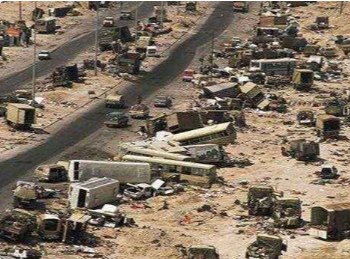
\includegraphics[scale=0.2]{figures/soft1}}\quad
				%\subfigure{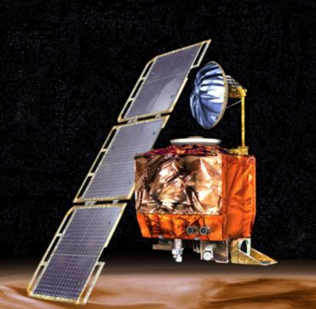
\includegraphics[scale=0.4]{figures/soft2}}
			  \subfigure{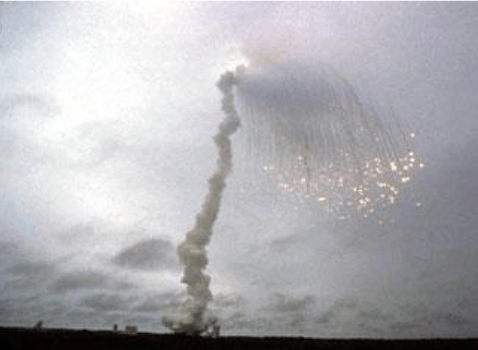
\includegraphics[scale=0.15]{figures/soft3}}\quad
				\subfigure{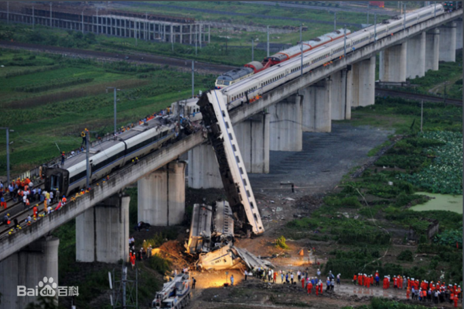
\includegraphics[scale=0.4]{figures/soft4}}
				\caption{系统故障引起的系列灾难现场}
			\end{figure}
		
			\begin{table}[htbp]
				\setlength{\abovecaptionskip}{-0.2cm}  %段前
				\setlength{\belowcaptionskip}{-0.4cm} %段后
				\fontsize{7pt}{\baselineskip}\selectfont
				\caption{由系统故障引起的重大事件概览}
				\label{tab:systemEvents_1.1}
				\centering
				\begin{tabular}{p{0.12\textwidth}p{0.35\textwidth}p{0.5\textwidth}}%
					\toprule
					\textbf{时间}&\textbf{事故原因}&\textbf{损失}\\
					\midrule
					1991年 & 美国爱国者导弹系统舍入错误 & 28名士兵死亡、100人受伤等\\
					1996年 & 阿丽亚娜5火箭 代码重用 & 火箭与其它卫星毁灭\\
					1999年 & 火星探测器用错度量单位 & 探测器坠毁并造成了3.27亿美元的损失\\
					2011年 & 温州7.23动车\underline{信号设备}在设计上存在严重的缺陷 &动车脱节脱轨、多人失去生命\\
					\bottomrule
				\end{tabular}
			\end{table}
	\end{frame}

	\begin{frame}
		\frametitle{研究背景和意义: {\small 形式化验证为系统的正确提供了有力依据}} 
\begin{block}{自动定理证明(Automated theorem proving)}
		\begin{columns}
		\column{0.5\textwidth}
			令$\phi_{imp}$和$\phi_{spec}$分别表示系统模型和规范对应的时序逻辑公式:
			\begin{itemize}
				\item $\phi_{imp} \rto \phi_{spec}$,或
				\item $\phi_{imp} \lrto \phi_{spec}$。
			\end{itemize}
		\column{0.5\textwidth}
			\begin{figure}
				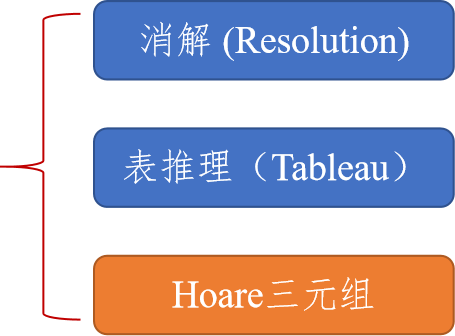
\includegraphics[scale=0.3]{figures/atp}
			\end{figure}
		\end{columns} 
	\begin{figure}
		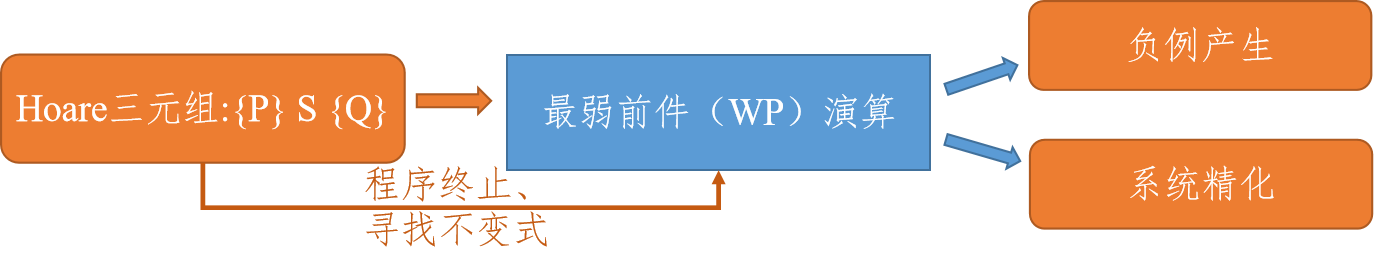
\includegraphics[scale=0.3]{figures/hoareTriple}
	\end{figure}
	\end{block}
\vskip 0.5pt
	\begin{block}{模型检测(Model Checking)}
		\begin{columns}
			\column{0.5\textwidth} 
			\begin{itemize}
				\item $\textcolor{red}{\Hm} \models^? \phi_{spec}$.
				\item {\small 反应式系统(reactive system):是指与环境有着持续不断交互的系统。}
				\item \textcolor{red}{如何计算反应式系统的WP?}
			\end{itemize}
			\column{0.5\textwidth}
			\begin{figure}
				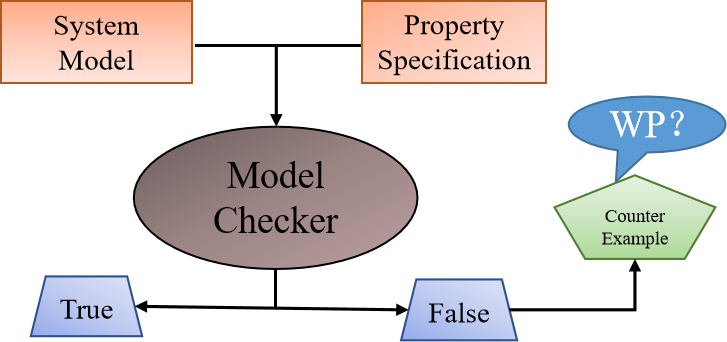
\includegraphics[scale=0.35]{figures/MC}
			\end{figure}
		\end{columns}
	\end{block}
	\end{frame}

\begin{frame}
	\frametitle{~研究背景和意义:{\small 例子}}
	{\scriptsize \begin{example}[汽车制造企业模型]\label{car_manufacturing}
		
			一个汽车制造企业能够生产两种汽车:小轿车($se$)和跑车($sp$)。每隔一段时间,该企业都会做一个生产决策($d$),即:合理的生产计划。
			刚开始的时候,该企业做出了具有三个选择($s$)的方案:
			\begin{itemize}
				\item[(1)] 先生产足够的$se$,然后在再生产$sp$;
				\item[(2)] 先生产足够的$sp$,然后再生产$se$;
				\item[(3)] 同时生产$se$和$sp$。
			\end{itemize}
		这一过程可以由图~\ref{BVM}中的Kripke结构(带标签的状态转换图)$\Hm=(S,R,L)$模拟。
		\begin{columns}
			\column{0.5\textwidth}
%			\begin{itemize}
%				\item $V=\{d,s, se, sp\}$为该工厂所需要考虑的原子命题集;
%				\item $S=\{s_0,s_1,s_2,s_3,s_4\}$为状态空间;
%				\item $R = \{(s_0, s_1), (s_1,s_2), (s_1,s_3), (s_1,s_4),
%				$ $(s_2,s_0),$ $(s_3,s_0),$ $(s_4,s_0)\}$ 为状态转换关系集;
%				\item $L: S \rto 2^V$为标签函数,具体地:$L(s_0) = \{d\}$、$L(s_1) = \{s\}$、 $L(s_2)=\{se\}$、 $L(s_3) = \{sp\}$和$L(s_4) = \{se,sp\}$。
%			\end{itemize}
	\begin{figure}
		\centering
		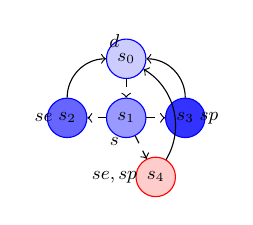
\begin{tikzpicture}[scale=0.75]
			\tikzstyle{every node}=[font=\small,scale=0.75]
			\node[blueCircle] (s0) at(0,1) {$s_0$};
			\node[blueCircle1] (s1) at(0,0) {$s_1$};
			\node[blueCircle2] (s2) at(-1,0) {$s_2$};
			\node[blueCircle3] (s3) at(1,0) {$s_3$};
			\node[redCircle] (s4) at(0.5,-1) {$s_4$}; 
			\draw[->,dashed] (s0) -- (s1);
			\draw[->,dashed] (s1) -- (s2);
			\draw[->,dashed] (s1) -- (s3);
			\draw[->,dashed] (s1) -- (s4);
			%	\draw[->] (s4) -- (s0);
			\path (s4) edge[->,bend right=45] (s0);
			\path (s2) edge[->,bend right=-45] (s0);
			\path (s3) edge[->,bend right=45] (s0);
			\node at(-0.2,1.3) {$d$};
			\node at(-1.4,0) {$se$};
			\node at(1.4,0) {$sp$};
			\node at(-0.2,-0.4) {$s$};
			\node at(-0.2,-1) {$se, sp$};
			%	\node at(0,-1.5) {${\cal K}_2$}; 
		\end{tikzpicture}
		\caption{{\tiny 汽车制造企业模型}}\label{BVM}
	\end{figure} 
			\column{0.5\textwidth}  
			\pause
			由于经济危机或者战略调整,导致该企业不能再生产跑车。这意味着所有规范和Kripke结构都不再需要考虑$sp$,因此应该\textcolor{blue}{“移除”}。
%			\begin{figure}
%				\centering
%			\begin{tikzpicture}[scale=0.75]
%				\tikzstyle{every node}=[font=\small,scale=0.75]
%				\node[blueCircle] (s0) at(0,1) {$s_0$};
%				\node[blueCircle1] (s1) at(0,0) {$s_1$};
%				\node[blueCircle2] (s2) at(-1,0) {$s_2$};
%				\node[blueCircle3] (s3) at(1,0) {$s_3$};
%				\node[redCircle] (s4) at(0.5,-1) {$s_4$}; 
%					\draw[->,dashed] (s0) -- (s1);
%					\draw[->,dashed] (s1) -- (s2);
%					\draw[->,dashed] (s1) -- (s3);
%					\draw[->,dashed] (s1) -- (s4);
%				%	\draw[->] (s4) -- (s0);
%					\path (s4) edge[->,bend right=45] (s0);
%					\path (s2) edge[->,bend right=-45] (s0);
%					\path (s3) edge[->,bend right=45] (s0);
%					\node at(-0.2,1.3) {$d$};
%					\node at(-1.4,0) {$se$};
%					\node at(1.4,0) {$sp$};
%					\node at(-0.2,-0.4) {$s$};
%					\node at(-0.2,-1) {$se, sp$};
%				%	\node at(0,-1.5) {${\cal K}_2$}; 
%			\end{tikzpicture}
%		\caption{{\tiny 汽车制造企业模型}}\label{BVM}
%			\end{figure}
%			 \begin{figure} 
%			 	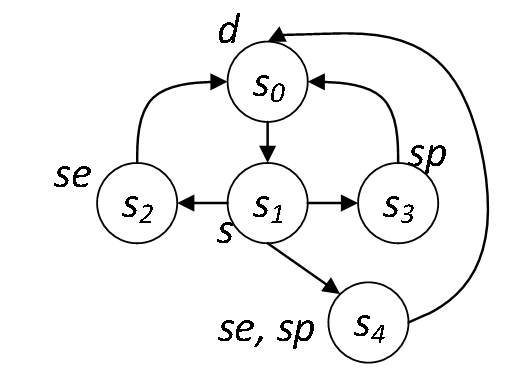
\includegraphics[width=3cm]{figures/NnewCar}
%			 	\caption{汽车制造企业模型}\label{BVM}
%			 \end{figure} 
		\end{columns} 
%		假定,由于经济危机或者战略调整,导致该企业不能再生产跑车。这意味着所有规范和Kripke结构都不再需要考虑$sp$的,因此应该\textcolor{blue}{“移除”}。
	\end{example}}
\end{frame}
	
	\begin{frame}
		\frametitle{~研究背景和意义: {\small 知识表示与推理(KR)中的SNC和WSC}}
		{\footnotesize 	
			\only<1>{
				\begin{block}{最强必要条件(SNC)和最弱充分条件(WSC)}
			SNC和WSC分别用于描述给定理论下的最一般的结果(consequence)和最一般的诱因(abduction)\cite{DBLP:journals/ai/Lin01}。满足下面两个条件的$\varphi$称为$q$在理论$\Sigma$下的SNC:
			\begin{itemize}
				\item[(1)] $\Sigma \models q \rto \varphi$;
				\item[(2)] 对任意$\varphi'$且$\Sigma \models q \rto \varphi'$,有$\Sigma \models \varphi \rto \varphi'$。
			\end{itemize}
		满足下面两个条件的$\psi$称为$q$在理论$\Sigma$下的(WSC):
		\begin{itemize}
			\item[(1)] $\Sigma \models \psi \rto q$; 
			\item[(2)] 对任意$\psi'$且$\Sigma \models \psi' \rto q$,有$\Sigma \models \psi' \rto \psi$。
		\end{itemize}
		\end{block}
		\vskip 0.5pt
 \begin{block}{遗忘理论(Forgetting)}
			\begin{columns}
				\column{0.5\textwidth} 
				 %在一阶逻辑中,从公式$\varphi$中遗忘掉一个$n$元谓词$P$的结果是$\exists R.\varphi[P/R]$,即将公式$\varphi$中的所有$P$的出现都用一个新的$n$元谓词$R$来替代。 
				 {\em 遗忘}是一种从理论中抽取知识的技术\cite{Fangzhen:forgetit},被用于\underline{规划}\cite{DBLP:conf/ijcai/DohertyLS01,lin2003compiling}和\underline{知识更新}中\cite{Yan:AIJ:2009}。
				 
				 在一阶逻辑中,从公式$\varphi$中遗忘掉一个$n$元谓词$P$的结果是$\exists R.\varphi[P/R]$,即将公式$\varphi$中的所有$P$的出现都用一个新的$n$元谓词$R$来替代。
				 %非形式化地,对于逻辑语言L中的任意公式和原子集合,如果从该公式中遗忘掉该原子集合后得到的结果仍然在L中,则称\textcolor{blue}{遗忘存在},同时也称该公式和原子集合的遗忘存在。
				\column{0.5\textwidth}
				\begin{figure}
					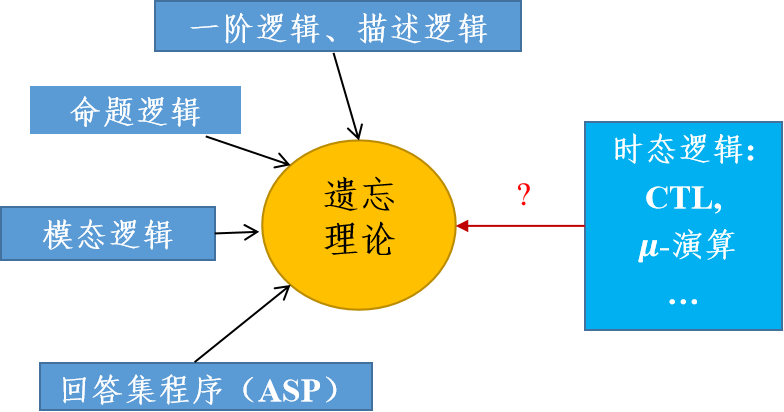
\includegraphics[scale=0.35]{figures/forgetting}
				\end{figure}
			\end{columns}
		\end{block}}
	\only<2>{
		\begin{figure}
			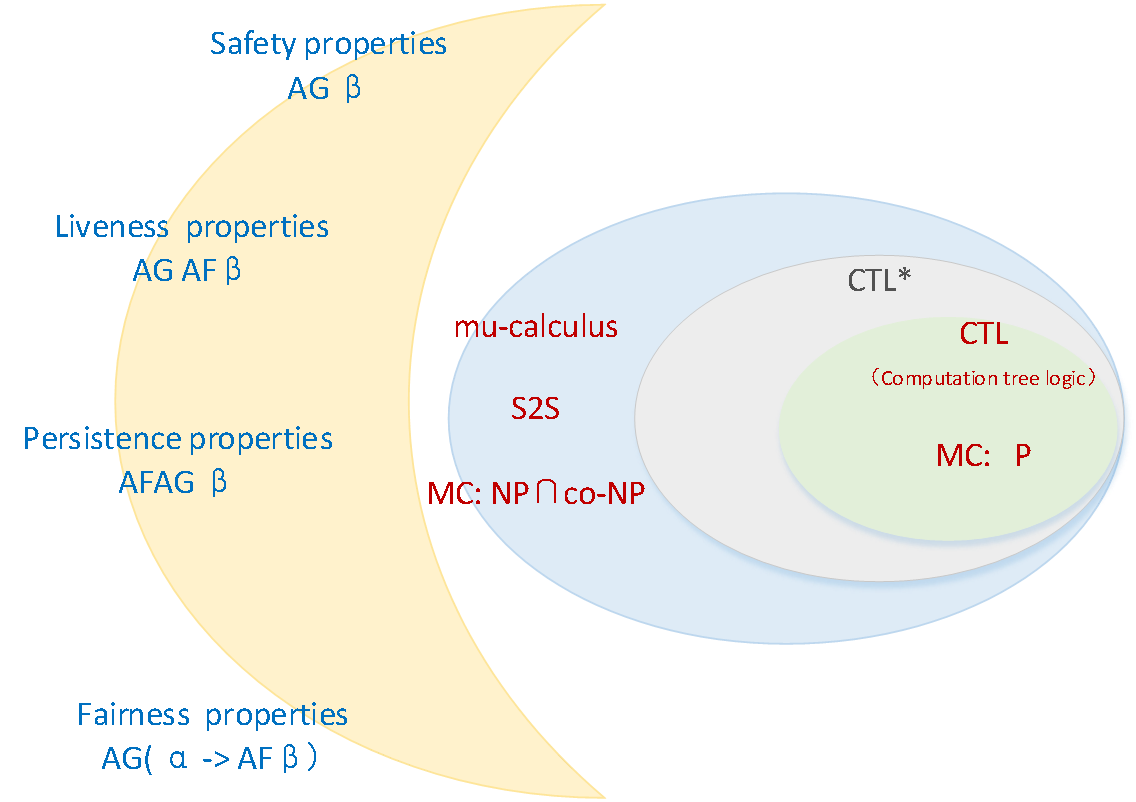
\includegraphics[scale=0.35]{figures/CTLmu}
		\end{figure}
%		\begin{itemize}
%			\item CTL(Computation tree logic):计算树逻辑,是一种分支时序逻辑
%			\begin{itemize}
%				\item 其模型检测(MC)问题能在多项时间内完成;
%				\item 能很好的表达系统要求的各种属性:安全属性(Safety properties)、活性属性(Liveness	properties)、持续属性(Persistence properties)和公平属性(Fairness properties)。
%				\begin{itemize}
%					\item \textcolor{orange!80}{安全属性(Safety properties)}:\textcolor{blue!70}{($\ALL \GLOBAL \neg \varphi$)}
%					%something bad never happens. \textcolor{blue!70}{($\ALL \GLOBAL \neg \varphi$)}
%					\item \textcolor{orange!80}{活性属性(Liveness	properties)}:\textcolor{blue!70}{($\ALL \GLOBAL \ALL \FUTURE \varphi$)}
%					%something good will eventually happen. \textcolor{blue!70}{($\ALL \GLOBAL \ALL \FUTURE \varphi$)}
%					\item \textcolor{orange!80}{持续属性(Persistence properties)}:\textcolor{blue!70}{($\ALL \FUTURE \ALL \GLOBAL \varphi$)}
%					%eventually for ever a certain proposition holds. \textcolor{blue!70}{($\ALL \FUTURE \ALL \GLOBAL \varphi$)}
%					\item \textcolor{orange!80}{公平属性(Fairness properties)}:\textcolor{blue!70}{(一种约束:在约束$fair = \GLOBAL \FUTURE a$下$\ALL \GLOBAL(a\rto \ALL \FUTURE b)$是否成立?)}
%				%	does, under certain conditions, an event occur repeatedly? \textcolor{blue!70}{(一种约束:在约束$fair = \GLOBAL \FUTURE a$下$\ALL \GLOBAL(a\rto \ALL \FUTURE b)$是否成立?)}
%				\end{itemize} 
%			\end{itemize}
%			\item $\mu$-演算($\mu$-calculus):是其他形式体系的机械基础
%			\begin{itemize}
%				\item LTL、CTL、$L_w$等时态逻辑都能用$\mu$-演算表示;
%				\item S1S表达能力严格不如$\mu$-演算;
%				\item $\mu$-演算与S2S有相同的表达能力;
%				\item ......
%			\end{itemize}
%		\end{itemize}  
\textcolor{red}{形成时序逻辑系统遗忘理论的框架,架起形式化验证(verification)和知识表示与推理(KR)的桥梁。}}
	}
	\end{frame}
	
	\subsection{国内外研究现状} 
	%\subsection*{国内研究现状}
	\begin{frame}
		\frametitle{~国内外研究现状}
		\begin{figure}
			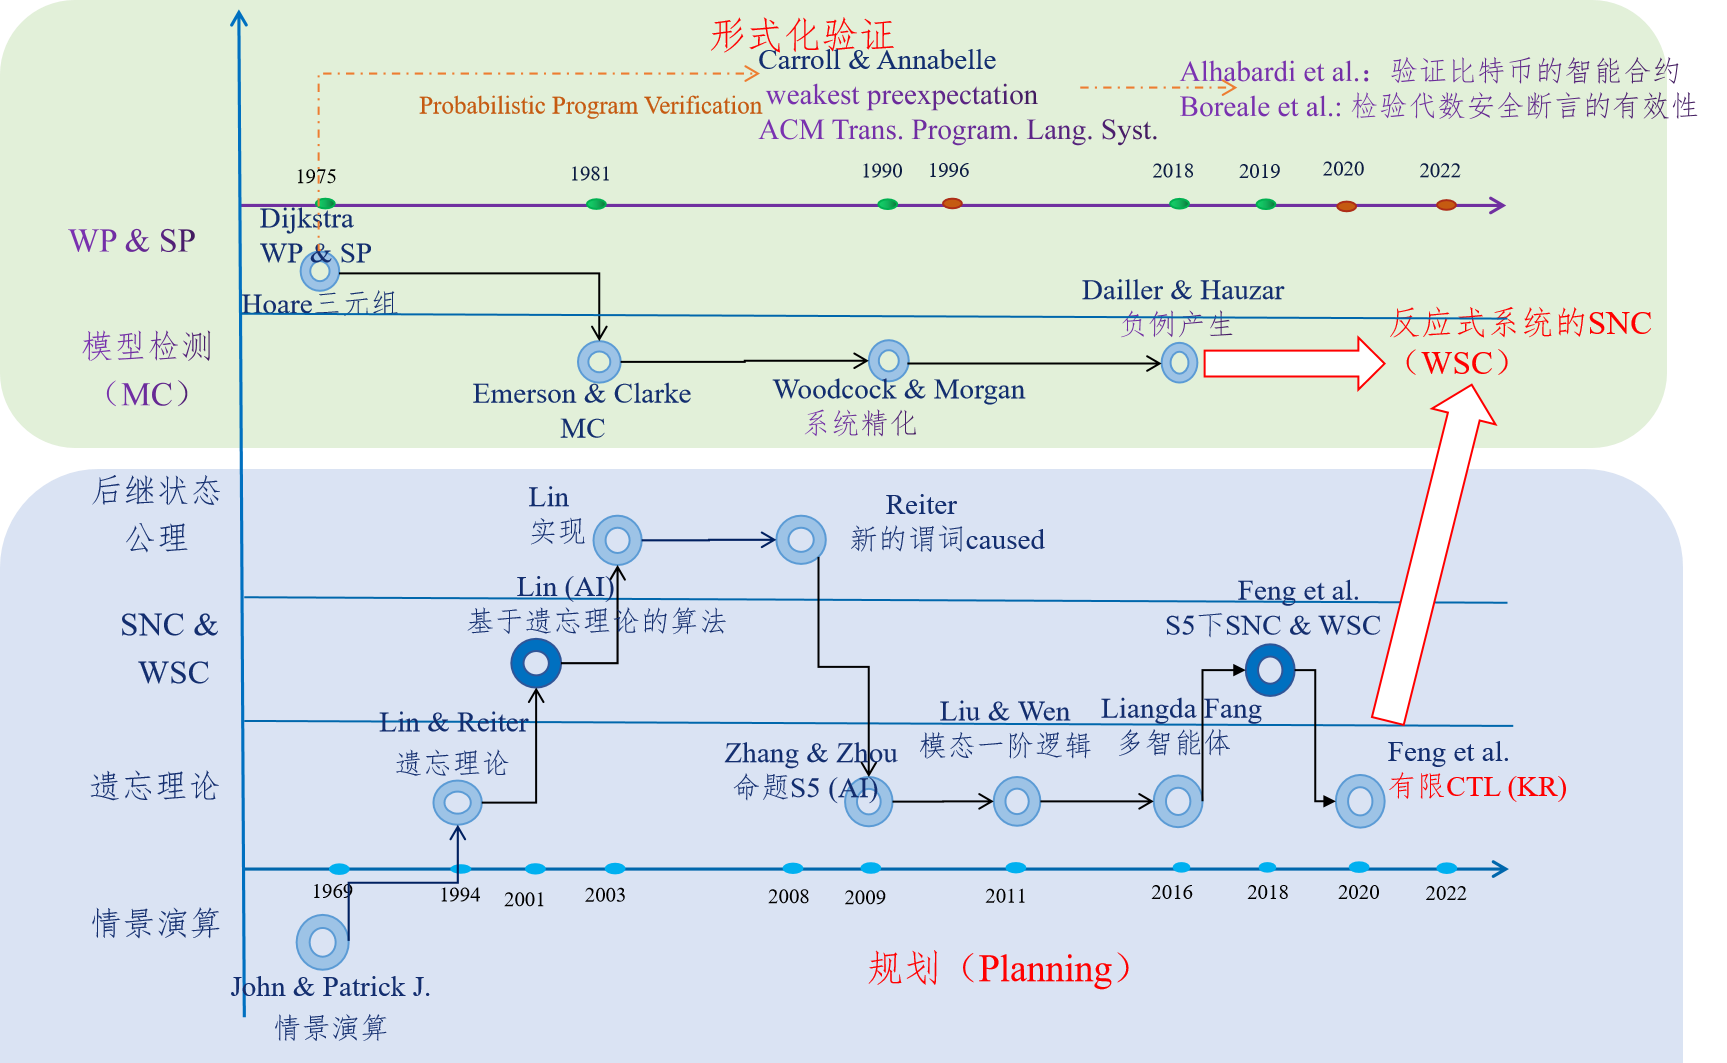
\includegraphics[scale=0.35]{figures/history2}
		\end{figure}
	\end{frame}

\subsection{研究目标}
	\begin{frame}
		\frametitle{~研究目标}
		\begin{figure}
			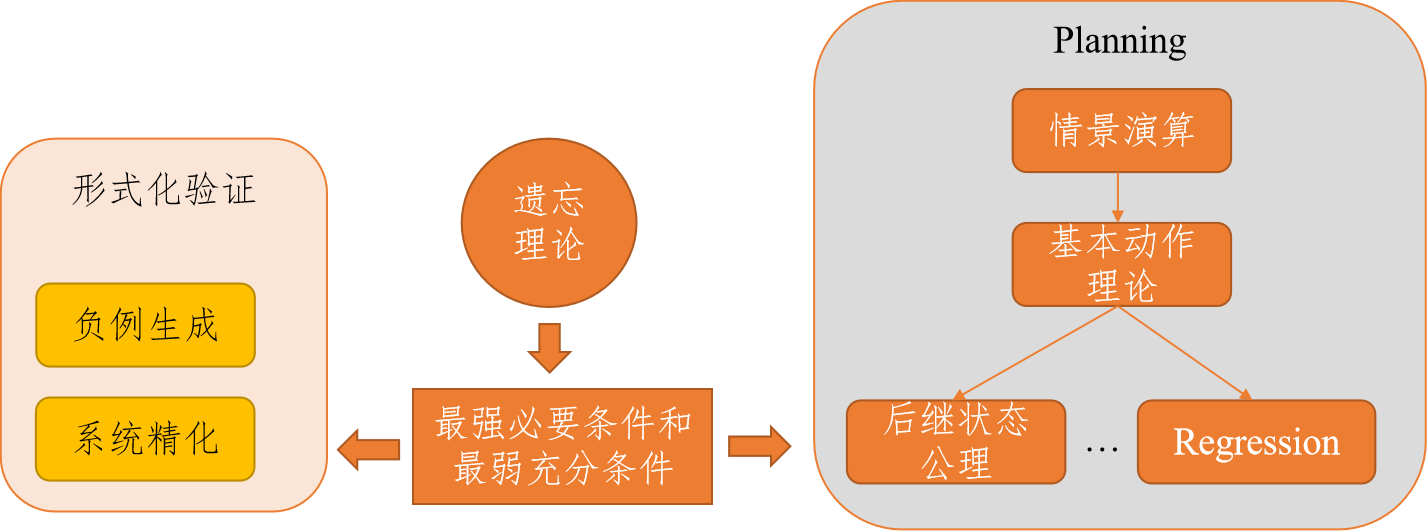
\includegraphics[scale=0.3]{figures/mubiao}
		%	\caption{文章组织结构示意图}
		\end{figure}
{\footnotesize
		通过人工智能的知识表示与推理(KR)技术,从{\em 遗忘理论}出发,研究{\em 反应式系统}(在某个符号集上)SNC和WSC的表示与计算,具体为:
		\begin{itemize}
			\item $\CTL$和$\mu$-演算遗忘理论框架;
			\item 使用遗忘计算反应式系统的SNC和WSC。
		\end{itemize}
}
	\end{frame}

	
	\subsection{研究内容}
%	\begin{frame}
%		\frametitle{~研究内容}
%		\begin{block}<1->{研究内容}
%			\setlength{\baselineskip}{16pt}
%			\uncover<1->{~~~本论文研究反应式系统下,$\CTL$和$\mu$-演算的遗忘理论,并使用遗忘计算WSC。具体为:}
%			\begin{itemize}
%				\vskip 8pt
%				\item<2-> $\CTL$和$\mu$-演算的遗忘理论
%				\begin{itemize}
%					\item $\CTL$的遗忘理论
%					\item $\mu$-演算的遗忘理论
%				\end{itemize}
%				\item<3-> 遗忘理论在反应式系统的形式化验证和知识更新中的应用
%				\begin{itemize}
%					\item 计算WSC和SNC
%					\item 定义知识更新
%				\end{itemize}
%				\item<4-> 计算$\CTL$遗忘的算法
%				\begin{itemize}
%					\item 基于模型的计算方法
%					\item 基于消解(resolution)的计算方法
%					\item 实现与实验分析
%				\end{itemize}
%			\end{itemize}
%		\end{block}
%	\end{frame}

\begin{frame}
	\frametitle{~研究内容}
	{\footnotesize 	\begin{itemize}
		\item  研究内容(一):$\CTL$和$\mu$-演算的遗忘理论
		\item 研究内容(二):遗忘理论在反应式系统的形式化验证和知识更新中的应用
		\item 研究内容(三):$\CTL$遗忘的计算方法
	\end{itemize}}
	\begin{figure}
		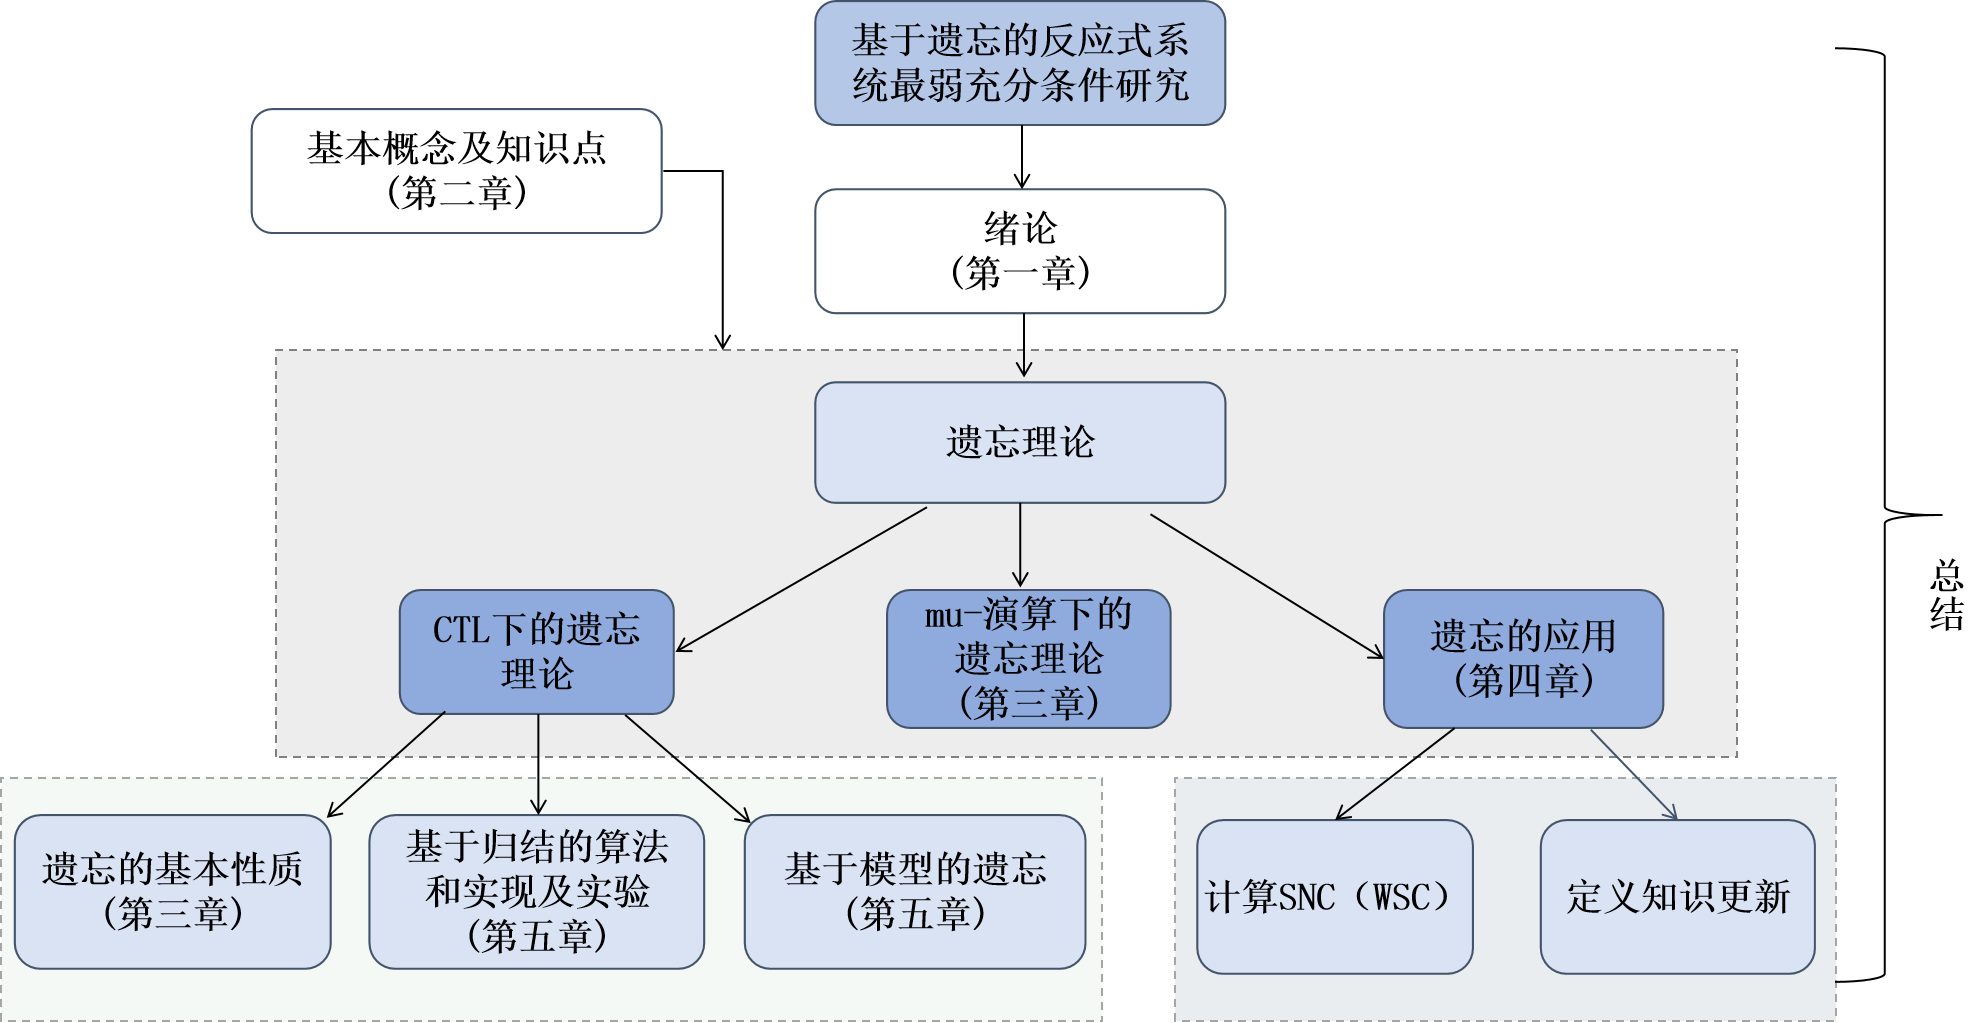
\includegraphics[scale=0.3]{figures/zuzhi}
		\caption{文章组织结构示意图}
	\end{figure}
\end{frame}


	
\section{研究内容(一):CTL和$\mu$-演算的遗忘理论}
%\subsection{CTL遗忘理论}  
\begin{frame}  
	\frametitle{~研究内容(一):CTL和$\mu$-演算的遗忘理论}
	\begin{figure}
		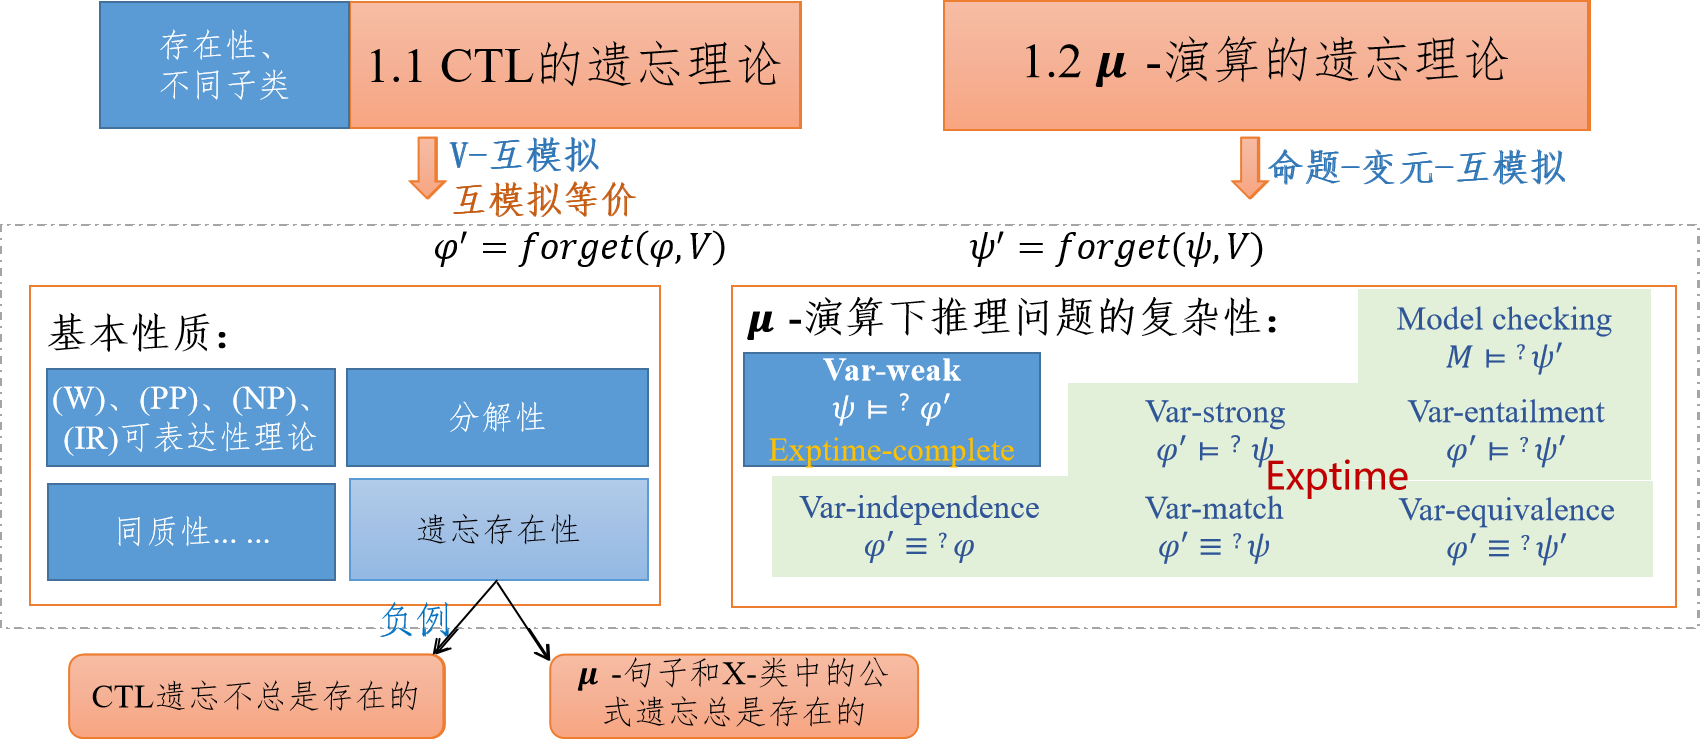
\includegraphics[scale=0.35]{figures/ctlMuForgFrame1}
		\caption{CTL和$\mu$-演算遗忘理论}
	\end{figure}
	{\tiny 
		\begin{columns}
			\column{0.5\textwidth}
			\begin{itemize} 
				\item 互模拟不变性:相互互模拟的结构满足相同的公式;
				\item (\W)、(\PP)、(\NgP)和(\IR):为遗忘理论公设;
			\end{itemize}
			\column{0.5\textwidth}
			\begin{itemize}
				%	\item 分解性:将一个大的问题分解成小的问题;
				\item 遗忘存在性:遗忘结果总是同一逻辑语言可表达的;
				\item $\varphi \models^? \psi$: 表示“$\varphi$是否逻辑蕴涵$\psi$”。
			\end{itemize}
		\end{columns}
	}

\end{frame}

\begin{frame}  
	\frametitle{~研究内容(一):CTL和$\mu$-演算的遗忘理论}
	\begin{figure}
		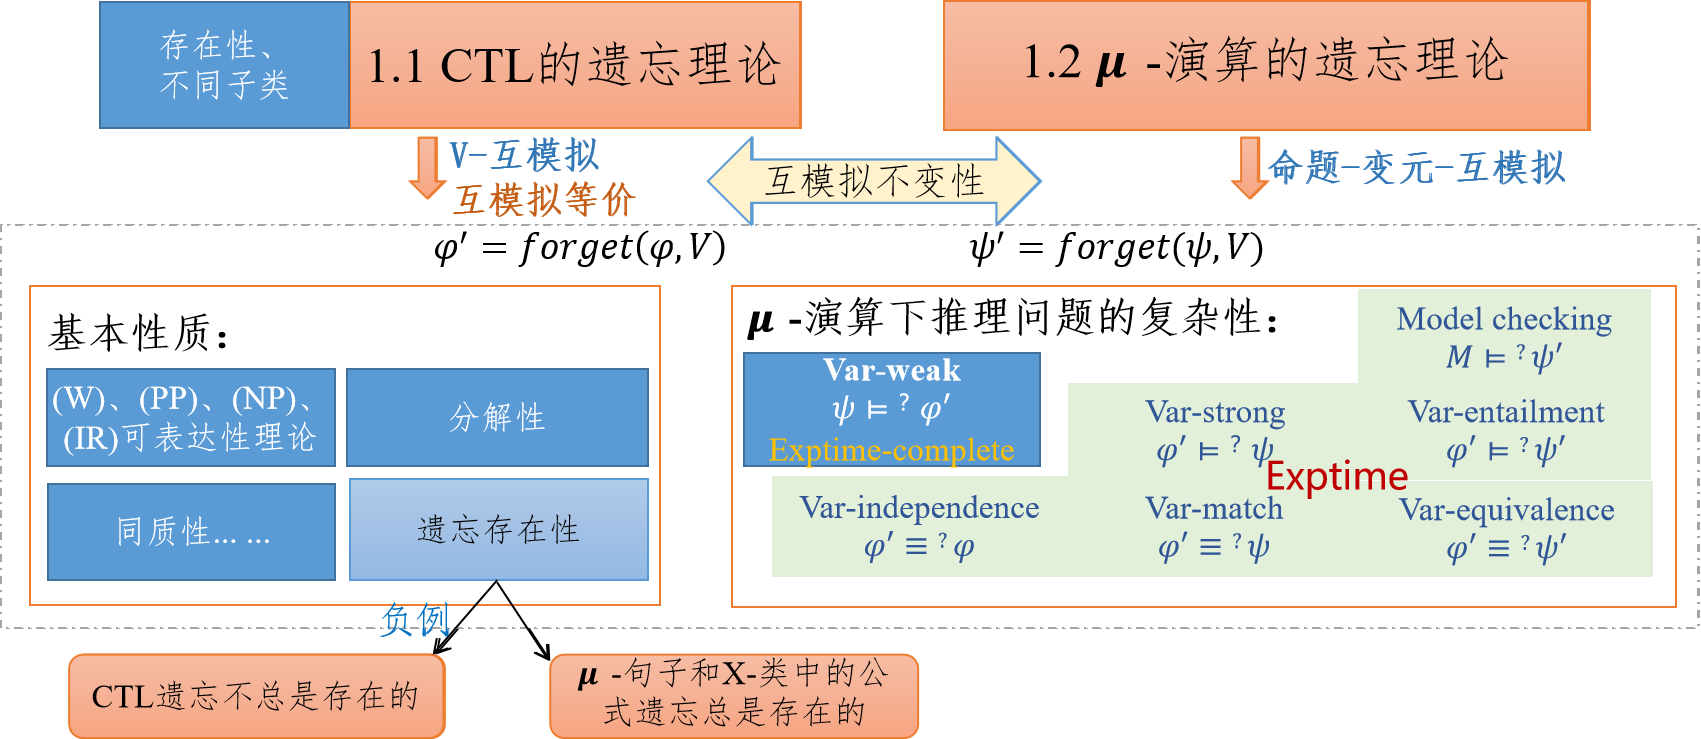
\includegraphics[scale=0.35]{figures/ctlMuForgFrame}
		\caption{CTL和$\mu$-演算遗忘理论}
	\end{figure}
	{\tiny 
		\begin{columns}
			\column{0.5\textwidth}
			\begin{itemize} 
				\item 互模拟不变性:相互互模拟的结构满足相同的公式;
				\item (\W)、(\PP)、(\NgP)和(\IR):为遗忘理论公设;
			\end{itemize}
			\column{0.5\textwidth}
			\begin{itemize}
				%	\item 分解性:将一个大的问题分解成小的问题;
				\item 遗忘存在性:遗忘结果总是同一逻辑语言可表达的;
				\item $\varphi \models^? \psi$: 表示“$\varphi$是否逻辑蕴涵$\psi$”。
			\end{itemize}
		\end{columns}
	} 
\end{frame}

\begin{frame}  
	\frametitle{~研究内容(一):CTL和$\mu$-演算的遗忘理论}
	\begin{figure}
		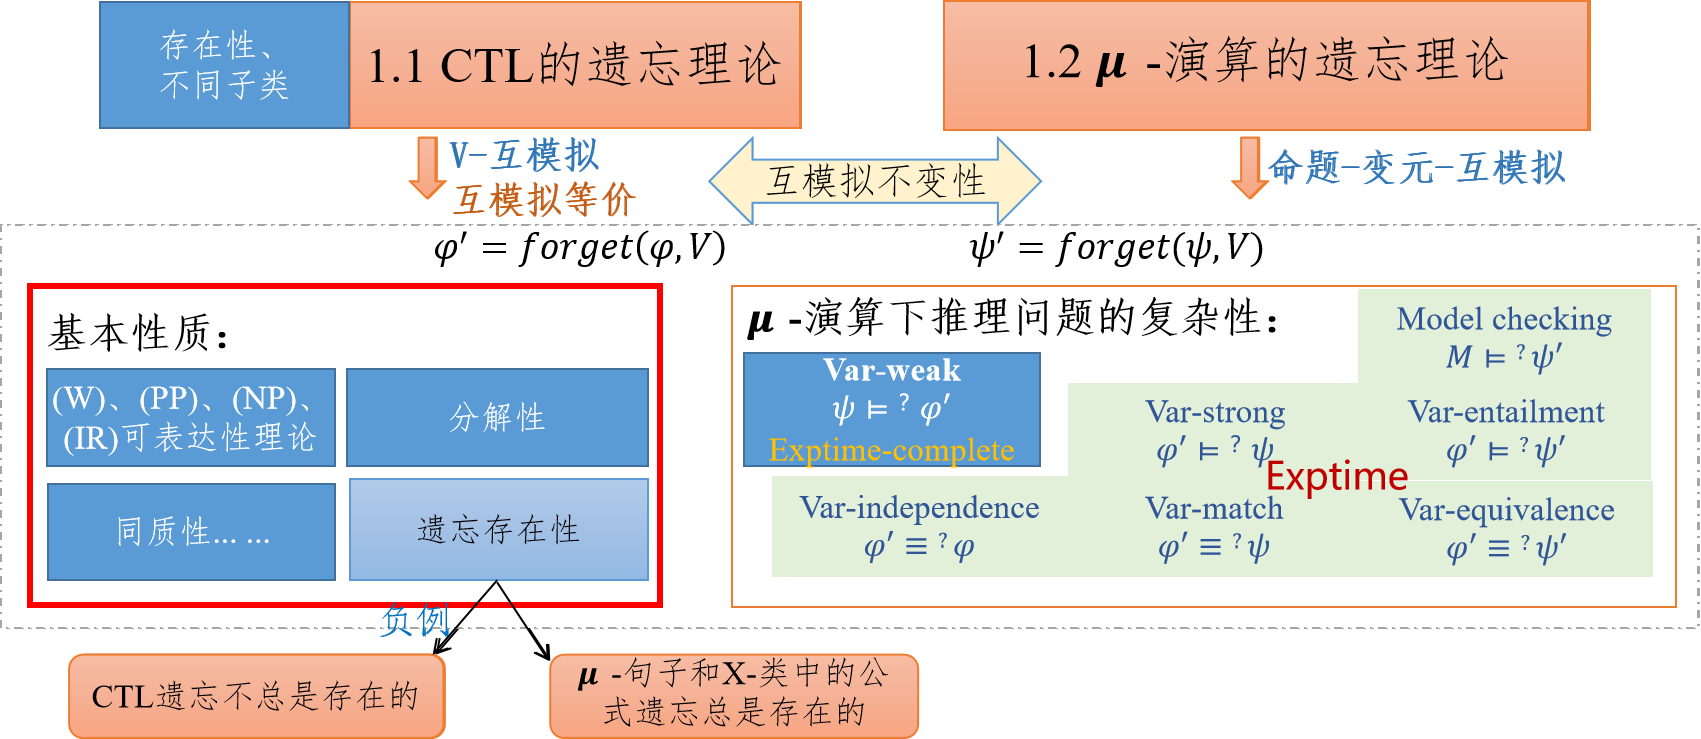
\includegraphics[scale=0.35]{figures/ctlMuForgFrame2}
		\caption{CTL和$\mu$-演算遗忘理论}
	\end{figure}
	{\tiny 
		\begin{columns}
			\column{0.5\textwidth}
			\begin{itemize} 
				\item 互模拟不变性:相互互模拟的结构满足相同的公式;
				\item (\W)、(\PP)、(\NgP)和(\IR):为遗忘理论公设;
			\end{itemize}
			\column{0.5\textwidth}
			\begin{itemize}
				%	\item 分解性:将一个大的问题分解成小的问题;
				\item 遗忘存在性:遗忘结果总是同一逻辑语言可表达的;
				\item $\varphi \models^? \psi$: 表示“$\varphi$是否逻辑蕴涵$\psi$”。
			\end{itemize}
		\end{columns}
	} 
\end{frame}

\begin{frame}  
	\frametitle{~研究内容(一):CTL和$\mu$-演算的遗忘理论}
	\begin{figure}
		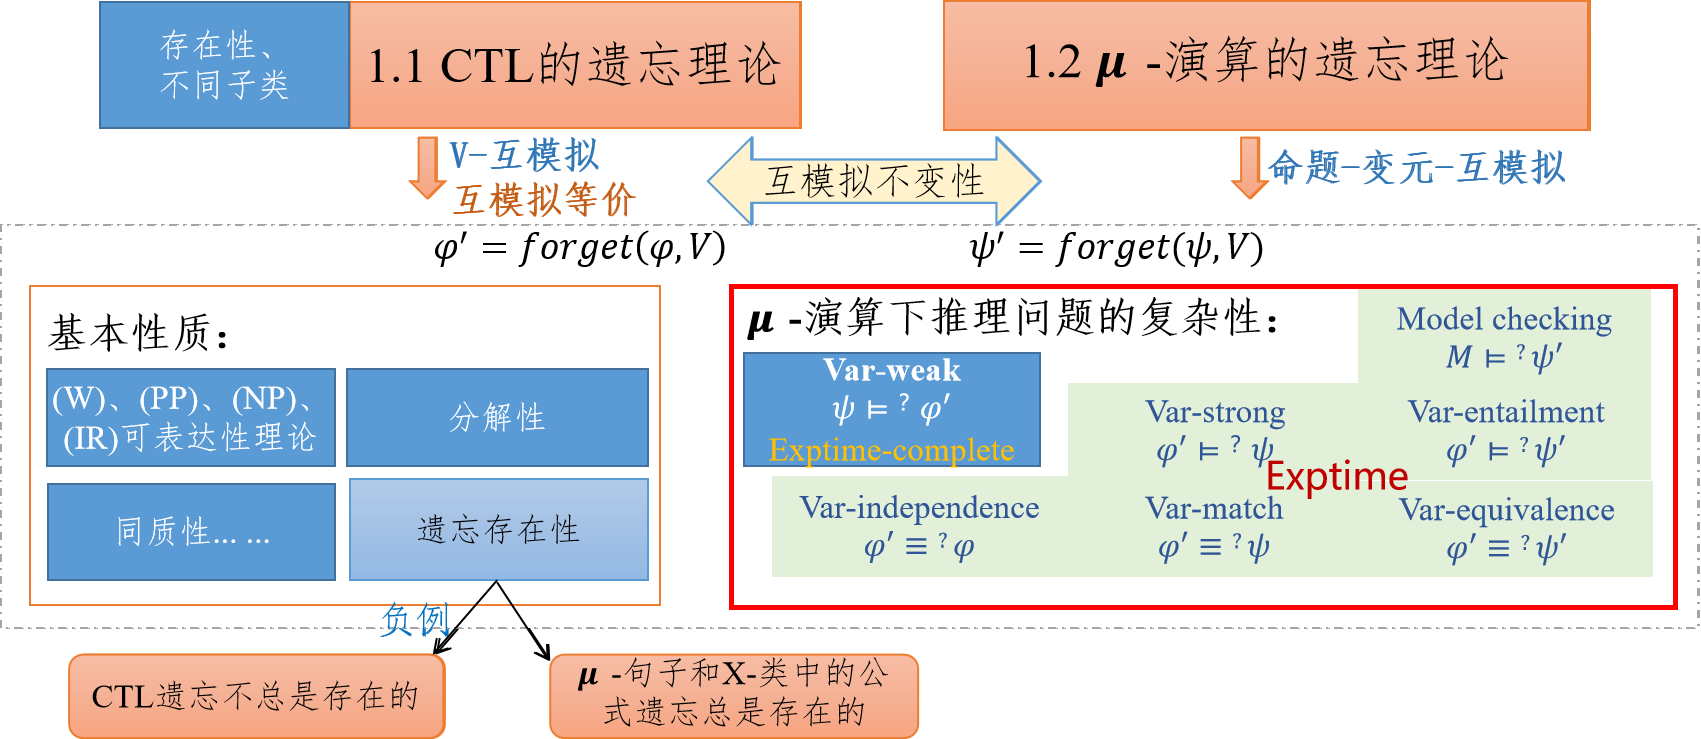
\includegraphics[scale=0.35]{figures/ctlMuForgFrame3}
		\caption{CTL和$\mu$-演算遗忘理论}
	\end{figure}
	{\tiny 
		\begin{columns}
			\column{0.5\textwidth}
			\begin{itemize} 
				\item 互模拟不变性:相互互模拟的结构满足相同的公式;
				\item (\W)、(\PP)、(\NgP)和(\IR):为遗忘理论公设;
			\end{itemize}
			\column{0.5\textwidth}
			\begin{itemize}
				%	\item 分解性:将一个大的问题分解成小的问题;
				\item 遗忘存在性:遗忘结果总是同一逻辑语言可表达的;
				\item $\varphi \models^? \psi$: 表示“$\varphi$是否逻辑蕴涵$\psi$”。
			\end{itemize}
		\end{columns}
	} 
\end{frame}

\begin{frame}  
	\frametitle{~研究内容(一):CTL和$\mu$-演算的遗忘理论}
	\begin{figure}
		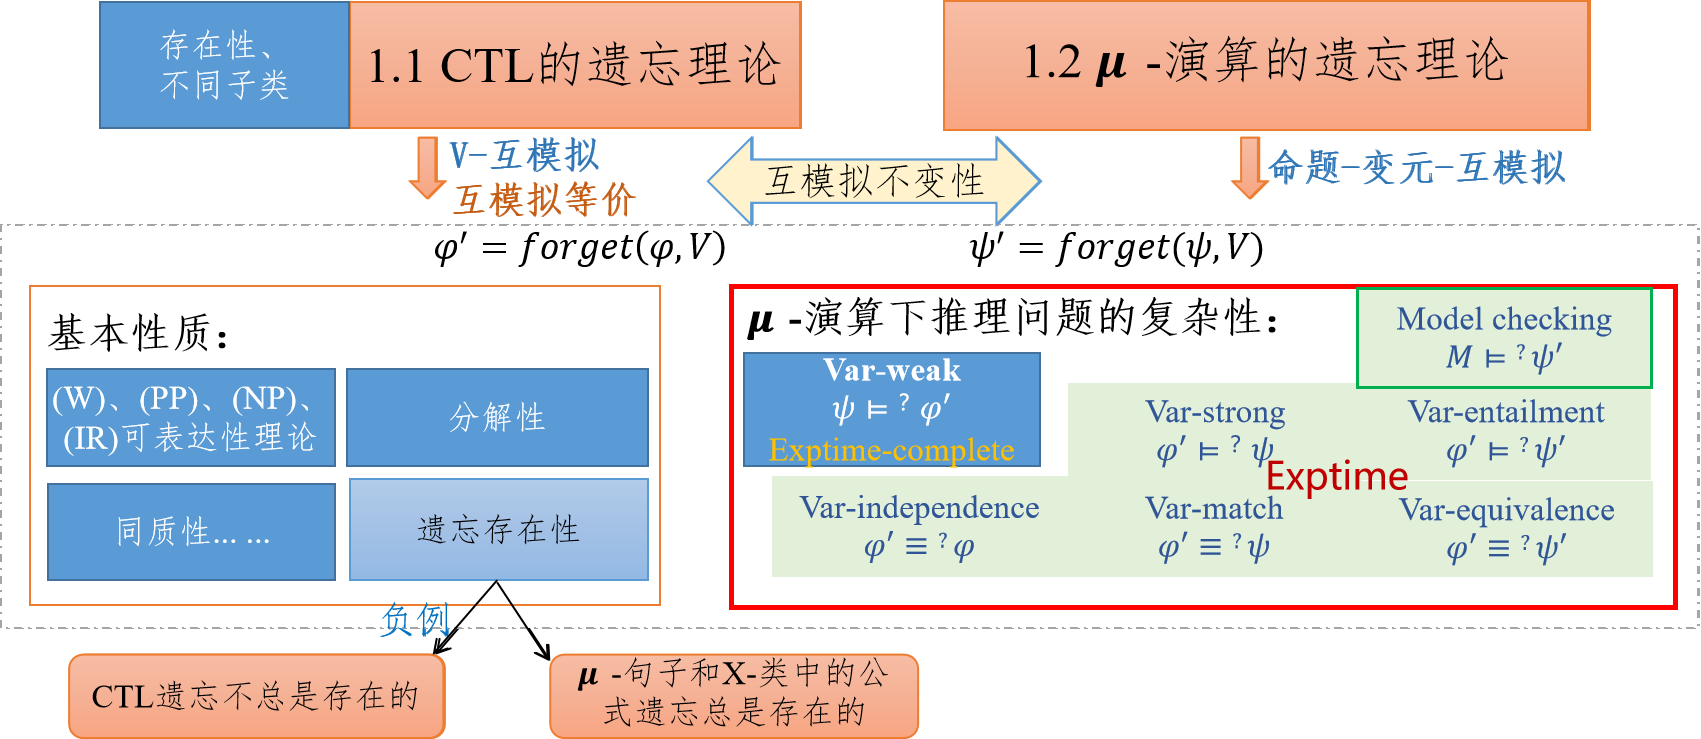
\includegraphics[scale=0.35]{figures/ctlMuForgFrame4}
		\caption{CTL和$\mu$-演算遗忘理论}
	\end{figure}
{\tiny 
	\begin{columns}
		\column{0.5\textwidth}
			\begin{itemize} 
				\item 互模拟不变性:相互互模拟的结构满足相同的公式;
				\item (\W)、(\PP)、(\NgP)和(\IR):为遗忘理论公设;
			\end{itemize}
		\column{0.5\textwidth}
			\begin{itemize}
			%	\item 分解性:将一个大的问题分解成小的问题;
				\item 遗忘存在性:遗忘结果总是同一逻辑语言可表达的;
				\item $\varphi \models^? \psi$: 表示“$\varphi$是否逻辑蕴涵$\psi$”。
			\end{itemize}
	\end{columns}
}
\pause

\textcolor{red}{\[\hbox{形成了时序逻辑遗忘理论的框架!}\]}
\end{frame}

%		
%	\begin{frame} 
%		\frametitle{~CTL遗忘理论——{\footnotesize 互模拟}}
%		{\scriptsize 
%			\begin{definition}[$V$-互模拟]
%				\label{def:VInd:bisimulation}
%				给定原子命题集$V\subseteq\cal A$、索引集合$I\subseteq \Ind$和初始$\Ind$-结构 $\Hm_i=(S_i, R_i,L_i, [\_]_i, s_0^i)~(i=1,2)$。
%				$\Hb_V \subseteq S_1 \times S_2$为二元关系,对任意$s_1 \in S_1$和$s_2 \in S_2$,若$(s_1, s_2)\in \Hb_V$,则:
%				\begin{itemize}[<+-| alert@+>]
%					\item[(i)] $L_1(s_1) - V = L_2(s_2) -V$;
%					\item[(ii)] $\forall r_1\in S_1$, 若$(s_1, r_1)\in R_1$,则$\exists r_2 \in S_2$ 使得 $(s_2,r_2) \in R_2$ 和 $(r_1, r_2) \in \Hb_V$;
%					\item[(iii)] $\forall r_2\in S_2$,若$(s_2, r_2)\in R_2$,则 $\exists r_1 \in S_1$ 使得 $(s_1,r_1) \in R_1$ 和 $(r_1, r_2)\in \Hb_V$。
%				\end{itemize}
%				那么,称 $\Hb_V$ 是 $\Hm_1$和 $\Hm_2$之间的一个 $V$-互模拟关系。
%			\end{definition}
%%		\only<1>{
%			\begin{columns}
%			\column{0.5\textwidth} 
%			\begin{itemize}
%				\item \textcolor{blue!80}{结构互模拟}:若$\Hm_1$和 $\Hm_2$之间存在一个 $V$-互模拟关系$\Hb_V$使得$(s_1, s_2)\in \Hb_V$,则称两个 $\Ind$-结构 ${\cal K}_1$ $= (\Hm_1, s_1)$ 和 ${\cal K}_2 = (\Hm_2, s_2)$ 是 $V$-{\em 互模拟}的,记为${\cal K}_1$ $\lrto_V {\cal K}_2$;
%				\item \textcolor{blue!80}{路径互模拟}:令$i\in \{1,2\}$,$\pi_i=(s_{i,1},$ $s_{i,2},\ldots)$ 为 $\Hm_i$ 上的路径,若对任意$j \ge 1$都有$ {\cal K}_{1,j} \lrto_V {\cal K}_{2,j}$,则称这两条路径是$V$-{\em 互模拟}的,记为$\pi_1 \lrto_V \pi_2$,其中 ${\cal K}_{i,j}=(\Hm_i,$ $s_{i,j})$。
%			\end{itemize}
%			\column{0.5\textwidth}
%				\begin{figure}
%				\centering
%				\begin{tikzpicture}[scale=0.75]
%					\tikzstyle{every node}=[font=\small,scale=0.75]
%					\begin{minipage}{.2\textwidth}
%						\node[blueCircle] (s0) at(0,1) {$s_0$};
%						\node[blueCircle1] (s1) at(0,0) {$s_1$};
%						\node[blueCircle3] (s2) at(-1,0) {$s_2$};
%						\node[redCircle] (s3) at(1,0) {$s_3$};
%						\node[redCircle] (s4) at(0.5,-1) {$s_4$}; 
%						\draw[->,dashed] (s0) -- (s1);
%						\draw[->,dashed] (s1) -- (s2);
%						\draw[->,dashed] (s1) -- (s3);
%						\draw[->,dashed] (s1) -- (s4);
%						%	\draw[->] (s4) -- (s0);
%						\path (s4) edge[->,bend right=45] (s0);
%						\path (s2) edge[->,bend right=-45] (s0);
%						\path (s3) edge[->,bend right=45] (s0);
%						\node at(-0.2,1.3) {$d$};
%						\node at(-1.4,0) {$se$};
%						\node at(1.4,0) {$sp$};
%						\node at(-0.3,-0.3) {$s$};
%						\node at(-0.2,-1) {$se, sp$};
%						\node at(-0.4, -0.6) {${\cal K}_1$};
%					\end{minipage}
%					\begin{minipage}{.2\textwidth}
%						\node[blueCircle] (s10) at(3,2) {$s_0$};
%						\node[blueCircle1] (s11) at(3,1) {$s_1$};
%						\node[blueCircle2] (s12) at(2,1) {$s_2$};
%						\node[redCircle] (s13) at(4,1) {$s_3'$};
%						\draw[->] (s10) -- (s11);
%						\draw[->] (s11) -- (s12);
%						\draw[->] (s11) -- (s13);
%						\path (s12) edge[->,bend right=-45] (s10);
%						\path (s13) edge[->,bend right=45] (s10);
%						%\draw[<->] (s0) -- (s12);
%						\node at(2.8,2.3) {$d$};
%						\node at(1.6,1.2) {$se$};
%						\node at(4.4,1) {$\emptyset$};
%						\node at(2.7,0.7) {$s$};
%						\node at(2.6,0.4) {${\cal K}_2$};
%					\end{minipage}
%				\begin{minipage}{.2\textwidth}
%					\node[blueCircle] (s20) at(3,-1) {$s_0$};
%					\node[blueCircle1] (s21) at(3,-2) {$s_1$};
%					\node[blueCircle3] (s22) at(2,-2) {$s_2'$};
%					\draw[->] (s20) -- (s21);
%					\draw[->] (s21) -- (s22);
%					\path (s22) edge[->,bend right=-45] (s20);
%					\node at(2.7,-0.7) {$d$};
%					\node at(1.6,-2) {$\emptyset$};
%					\node at(2.7,-1.4) {$s$};
%					\node at(3.4,-2) {${\cal K}_3$};
%				\end{minipage}
%			\draw[<->,dashed] (s0) -- (s12);
%			\node at(1,1.1) {{\tiny $\{j\}$-互模拟}};
%			\draw[<->,dashed] (s11) -- (s20);
%			\node at(3,0) {{\tiny $\{se\}$-互模拟}};
%			\draw[<->,dashed] (s4) -- (s22);
%			\node at(1,-1.5) {{\tiny $\{se,sp\}$-互模拟}};
%					%	\node at(0,-1.5) {${\cal K}_2$}; 
%				\end{tikzpicture}
%				\caption{{\tiny 汽车制造企业模型}} 
%			\end{figure}
%%			\begin{figure}
%%				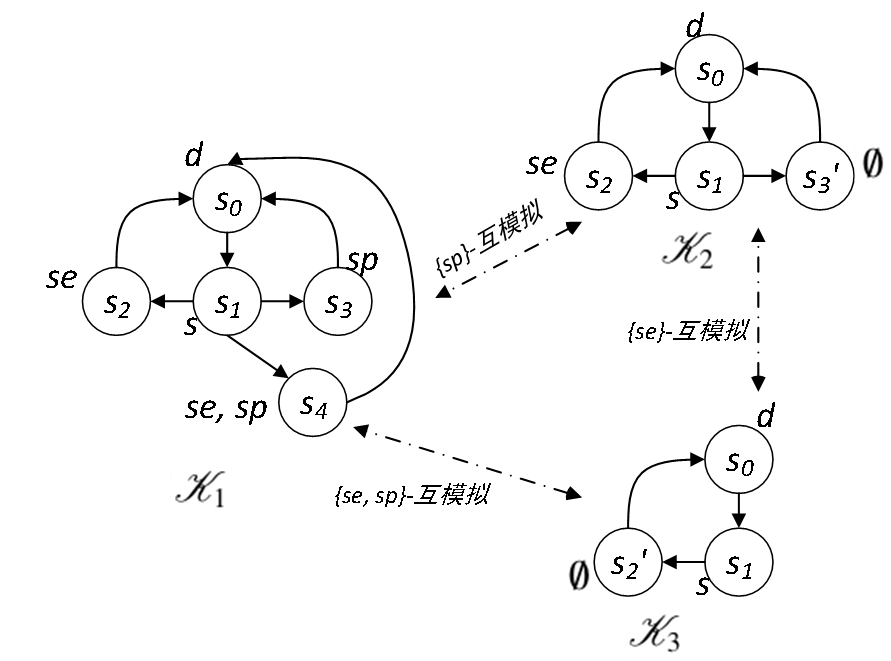
\includegraphics[scale=0.34]{figures/NVBnewCar1}
%%			\end{figure}
%		\end{columns}
%	%}
%%	\only<2>{
%%	%	\begin{block}{相关性质 1} 
%%			\begin{proposition}
%%				给定集合$V_i\subseteq \Ha$、状态$s_i'$、路径$\pi_i'$和$\Ind$-结构${\cal K}_j=(\Hm_j,s_j)$,其中$i=1,2$,$j=1,2,3$。 
%%				如果${\cal K}_1 \lrto_{V_1} {\cal K}_2$且${\cal K}_2 \lrto_{V_2} {\cal K}_3$,则:
%%				\begin{itemize}
%%					\item[(i)] ${\cal K}_1\lrto_{V_1\cup V_2}{\cal K}_3$;
%%					\item[(ii)] 若 $V_1 \subseteq V_2$,则 ${\cal K}_1 \lrto_{V_2} {\cal K}_2$;
%%					\item[(iii)] $s_1'\lrto_{V_i}s_2'~(i=1,2)$ 蕴涵$s_1'\lrto_{V_1\cup V_2}s_2'$;
%%					\item[(iv)] $\pi_1'\lrto_{V_i}\pi_2'~(i=1,2)$ 蕴涵 $\pi_1'\lrto_{V_1\cup V_2}\pi_2'$;
%%					\item[(v)] 对$\Hm_1$上的每条路径 $\pi_{s_1}$,存在$\Hm_2$上的一条路径 $\pi_{s_2}$ 使得 $\pi_{s_1} \lrto_{V_1} \pi_{s_2}$,反之也成立。
%%				\end{itemize}
%%			\end{proposition}
%%	%	\end{block}
%%	}
%%	\only<2>{
%%		\begin{theorem}[互模拟不变性]\label{thm:V-bisimulation:EQ}
%%			令$V\subseteq \Ha$是原子命题集,${\cal K}_i$ $(i=1,2)$是两个具有$V$-互模拟关系的$\Ind$-结构,即:${\cal K}_1 \lrto_V {\cal K}_2$。若$\Phi$是一个$\CTL$公式且$\IR(\Phi, V)$,则有${\cal K}_1\models \Phi$当且仅当${\cal K}_2\models \Phi$。
%%		\end{theorem}
%%	}
%		}
%	\end{frame}
%
%\begin{frame}
%	\frametitle{~CTL遗忘理论——{\footnotesize 互模拟等价}}
%	{\footnotesize
%%			\begin{theorem}[互模拟不变性]\label{thm:V-bisimulation:EQ}
%%			令$V\subseteq \Ha$是原子命题集,${\cal K}_i$ $(i=1,2)$是两个具有$V$-互模拟关系的$\Ind$-结构,即:${\cal K}_1 \lrto_V {\cal K}_2$。若$\Phi$是一个$\CTL$公式且$\IR(\Phi, V)$,则有${\cal K}_1\models \Phi$当且仅当${\cal K}_2\models \Phi$。
%%		\end{theorem}\pause
%		\begin{definition}[互模拟等价,bisimilar equivalence]\label{def:bisimular:equivalene}
%			给定原子命题集$V\subseteq {\cal A}$,公式$\varphi$和$\psi$。若对任意${\cal K}\models \varphi$,都存在一个${\cal K}'\models\psi$,使得${\cal K}\lrto_V{\cal K}'$;且对任意${\cal K}'\models\psi$,都存在一个${\cal K}\models \varphi$,使得${\cal K}\lrto_V{\cal K}'$,则称公式$\varphi$和 $\psi$是 {\em $V$-互模拟等价的(bisimilar equivalence)},记为 $\varphi\equiv_V\psi$。
%		\end{definition}
%	%\pause
%%\begin{lemma}~\label{lem:eqR}
%%		对任意$V\subseteq\cal A$,  $\lrto_V$和 $\equiv_V$为等价关系。
%%	\end{lemma}
%%\only<2>{
%%	\begin{corollary}~\label{cor:eqbi}
%%		令 $V$、$V_1$、$V_2$ 为$\cal A$的子集,$\varphi$和 $\psi$为公式。
%%		\begin{itemize}
%%			\item[(i)] 若 $\varphi\equiv\psi$,则 $\varphi\equiv_V\psi$。
%%			\item[(ii)] 若$\varphi$ 和 $\psi$不包括索引,且 $\varphi\equiv_\emptyset\psi$, 则 $\varphi\equiv\psi$。
%%			\item[(iii)] 若 $\varphi\equiv_{V_i}\psi~(i=1,2)$,则 $\varphi\equiv_{V_1\cup V_2}\psi$。
%%			\item[(iv)] 若 $\varphi\equiv_{V_1}\psi$ 和 $V_1\subseteq V_2$,则 $\varphi\equiv_{V_2}\psi$。
%%		\end{itemize}
%%	\end{corollary}
%%}
%\pause
%	\begin{proposition}\label{prop:transform:V:EQ}
%		令 $\varphi$为一个$\CTL$公式。则$\varphi\equiv_UT_\varphi$,其中 $T_\varphi=\CTLsnf(\varphi)$和
%		$U=\Var(T_\varphi)-\Var(\varphi)$。
%	\end{proposition}
%	}
%\end{frame}
%
%\begin{frame}
%	\frametitle{~CTL遗忘理论——{\footnotesize 定义}}
%	{\footnotesize 
%		\begin{definition}[遗忘,forgetting]\label{def:V:forgetting}
%			令$V$是$\Ha$的子集,$\Phi$是公式。如果公式$\psi$满足下面条件: 
%			\begin{itemize}
%				\item $\psi$与$V$中的原子命题无关(即:$\IR(\psi, V)$);
%				\item $\Mod(\psi)=\{{\cal K}\mid {\cal K} \mbox{是一个初始$\Ind$-结构}, \exists {\cal K}'\in\Mod(\phi)\ \text{使得}\ {\cal K}'\lrto_V{\cal K}\}$。
%			\end{itemize}  
%			那么,称$\psi$为从$\Phi$中遗忘$V$后得到的结果,记为$\CTLforget(\phi,V)$。
%		\end{definition}
%	\only<1>{\begin{block}{遗忘理论公设}
%		给定$\CTL$公式$\varphi$、$\varphi'=\CTLforget(\varphi, V)$、原子命题集$V\subseteq \Ha$和$\varphi'=\CTLforget(\varphi, V)$,$\CTL$下遗忘理论公设如下:
%		\begin{itemize}
%			\item[(\W)] 削弱:$\varphi \models \varphi'$;
%			\item[(\PP)] 正支持:对任意与$V$无关的公式$\eta$,若$\varphi \models \eta$则$\varphi' \models \eta$;
%			\item[(\NgP)] 负支持:对任意与$V$无关的公式$\eta$,若$\varphi \not \models \eta$则$\varphi' \not \models \eta$;
%			\item[(\textbf{IR})] 无关性: $\IR(\varphi', V)$。
%		\end{itemize}
%	\end{block}}
%	}
%\end{frame}
%
%\begin{frame}
%	\frametitle{~CTL遗忘理论——{\footnotesize 相关性质}}
%	{\footnotesize 
%		\only<1>{
%			\begin{theorem}[表达性定理,Representation Theorem]\label{thm:close} 
%				给定$\CTL$公式$\varphi$和$\varphi'$,$V \subseteq \Ha$为原子命题集。 
%				下面的陈述是等价的:
%				\begin{itemize}
%					\item[(i)] $\varphi' \equiv \CTLforget(\varphi, V)$,
%					\item[(ii)] $\varphi'\equiv \{\phi \mid\varphi \models \phi \text{和} \IR(\phi, V)\}$,
%					\item[(iii)] 若$\varphi$、$\varphi'$和$V$与(i)和(ii)中提到的符号相同,则公设(\W)、(\PP)、(\NgP)和(\textbf{IR})成立。
%				\end{itemize}
%			\end{theorem}
%		}
%	\only<2>{
%		\begin{example}\label{exp:e1}
%			令$p$和 $x$为两个不同的原子命题,$\varphi(p,x)$\footnote{$\varphi(p,x)$ 表示具有原子命题集$\Var(\varphi)=\{p,x\}$的公式。}为下面公式合取~\cite{Maksimova:JANCL:1991}:
%			\begin{align*}
%				&\ALL\GLOBAL(\neg x \wedge \neg \ALL \GLOBAL p \rto \neg \ALL \NEXT \neg x),
%				\qquad \ALL\GLOBAL(\neg \ALL\NEXT \neg x \rto \ALL \NEXT x),\\
%				& \ALL\GLOBAL(\ALL\NEXT x \rto \neg x \wedge \neg \ALL \GLOBAL p),
%				\qquad \ALL\GLOBAL(x \rto \neg \ALL\GLOBAL p),
%				\qquad \ALL\GLOBAL(\ALL \FUTURE \ALL \GLOBAL p).
%			\end{align*}
%			Maksimova证明了$\varphi(p,x)\land \varphi(p,y)\models x\lrto y$,且不存在$\CTL$公式 $\psi$使得 $\Var(\psi)=\{p\}$且$\varphi(p,x)$ $\models x\lrto \psi$,即$\CTL$不具有Beth性质。
%		\end{example}
%%	}
%%	\only<2,3>{
%		\begin{proposition}\label{pro:uniforget}
%			$\CTLforget(x\land \varphi(p,x), \{x\})$ 在 $\CTL$中是不可表示的。
%		\end{proposition}
%	\begin{theorem}\label{thm:PL:CTL}
%		给定一个命题公式$\varphi$和原子命题集$V\subseteq \Ha$,则下面逻辑等式成立。
%		\[\CTLforget(\varphi, V) \equiv \Forget(\varphi,V).
%		\]
%	\end{theorem}
%	}
%	\only<3>{
%%	\begin{lemma}\label{lem:KF:eq}
%%		给定两个公式$\varphi$和$\alpha$,原子命题$q \not \in (\Var(\varphi) \cup \Var(\alpha))$,则:$$\CTLforget(\varphi \wedge (q \lrto \alpha), q)\equiv \varphi.$$
%%	\end{lemma}
%\begin{proposition}[分解性,Decomposition]\label{disTF}
%	对于给定的公式$\varphi$,原子命题集$V$,和原子命题$p$($p\not \in V$),下面的结论成立:
%\begin{itemize}
%	\item $\CTLforget(\varphi,\{p\}\cup V) \equiv \CTLforget(\CTLforget(\varphi,p),V)$;
%	\item $	\CTLforget(\varphi,V_1\cup V_2) \equiv \CTLforget(\CTLforget(\varphi,V_1),V_2)$.
%\end{itemize} 
%\end{proposition}
%\begin{proposition}[同质性]\label{pro:ctl:forget:2}
%	令${\cal T} \in \{\NEXT, \FUTURE, \GLOBAL\}$、${\cal P} \in \{\ALL, \EXIST\}$,$\phi$为$\CTL$公式,且$P\subseteq\cal A$为原子命题集,则:
%	$$\CTLforget({\cal P}{\cal T}\phi,P)\equiv {\cal P}{\cal T} \CTLforget(\phi,P).$$
%\end{proposition}
%	}
%	}
%\end{frame}
%
%\begin{frame}
%	\frametitle{$\mu$-演算遗忘理论——{\footnotesize 变元-命题-互模拟}}
%	{\footnotesize
%	%	$\Hm_i = (S_i, R_i,L_i, r_i)~(i=1,2)$.
%		\only<1>{\begin{definition}[$V$-互模拟]\label{def:VB}
%			给定原子命题集$V \subseteq \Ha$和两个Kripke结构$\Hm_1$和 $\Hm_2$,其中$\Hm_i = (S_i, R_i,L_i, r_i)~(i=1,2)$。若$\Hb\subseteq S_1 \times S_2$满足下面几个条件:
%			\begin{itemize}
%				\item \fbox{\textcolor{red}{$r_1 \Hb r_2$,}}
%				\item 对任意$s\in S_1$和 $t\in S_2$,若$s \Hb t$,则对任意$p \in \Ha- V$,有$p \in L_1(s)$当且仅当 $p \in L_2(t)$,
%				\item 若$(s, s')\in R_1$和 $s \Hb t$,则存在一个 $t'$,使得$s' \Hb t'$和 $(t, t')\in R_2$,且
%				\item 若 $s \Hb t$和$(t, t')\in R_2$,则存在一个$s'$,使得$(s, s')\in R_1$和 $t' \Hb s'$。
%			\end{itemize}
%			则称$\Hb$是$\Hm_1$和 $\Hm_2$的$V$-互模拟关系。
%			
%				$\Hm_1 \lrto_V \Hm_2$、$(\Hm_1,$ $r_1) \lrto_V (\Hm_2,r_2)$:如果$\Hm_1$和 $\Hm_2$之间存在一个$V$-互模拟关系。
%		\end{definition}
%%	如果$\Hm_1$和 $\Hm_2$之间存在一个$V$-互模拟关系,那么${\cal B}$则称这两个Kripke结构$\Hm_1$和 $\Hm_2$及由这两个Kripke结构构成的结构$(\Hm_1,r_1)$和$(\Hm_2,r_2)$是$V$-互模拟的,分别记为$\Hm_1 \lrto_V \Hm_2$和$(\Hm_1,$ $r_1) \lrto_V (\Hm_2,r_2)$。
%}
%	\only<2>{
%		\begin{example}[不变性反例]\label{ex:2}
%			令$\varphi=\ALL\NEXT \neg X \lor \ALL \NEXT X$,$(\Hm,v)$和 $(\Hm',v')$为赋值,其中$\Hm=(S,r,R,L)$、$\Hm'=(S',r',R',L')$且
%			\begin{align*}
%				& S=\{r, r_1\}, R=\{(r,r_1)\}, L(r) = L(r_1) = \emptyset, v(X) = \{r_1\},\\
%				& S'=\{r', r_1',r_2'\}, R'=\{(r',r_1'),(r',r_2')\}, L(r') = L(r_1') = L(r_2')=\emptyset, v'(X) = \{r_1'\}.
%			\end{align*}
%			$\Hb=\{(r, r'), (r_1, r_1'), (r_1,r_2')\}$是$\Hm$和$\Hm'$之间的一个 $\emptyset$-互模拟。
%			
%			但是,\fbox{$(\Hm,v) \models \varphi$而$(\Hm',v') \not \models \varphi$}。 
%			\begin{figure}
%				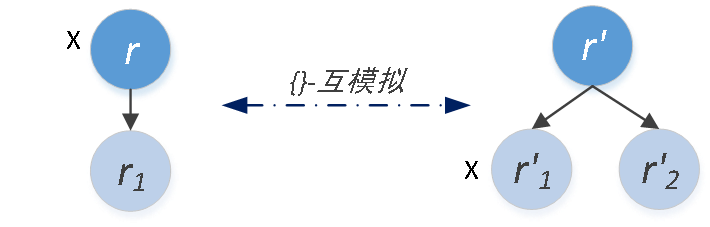
\includegraphics[scale=0.35]{figures/counterEVBmu}
%			\end{figure} 
%		\end{example}
%	}
%	\only<3>{
%		\begin{definition}[变元-命题-互模拟]
%			给定$V \subseteq \Ha$、${\cal V}_1 \subseteq {\cal V}$、$\Hm_i = (S_i, r_i, R_i, L_i)$为Kripke结构、 $s_i\in S_i$且
%			$v_i: {\cal V} \rto 2^{S_i}$,其中$i\in\{1,2\}$。若关系$\Hb\subseteq S_1 \times S_2$满足:
%			\begin{itemize}
%				\item $(s_1,s_2)\in\Hb$,
%				\item $\Hb$是$\Hm_1$ 和$\Hm_2$之间的$V$-互模拟,且
%				\item \textcolor{red}{对任意$(t_1,t_2)\in \Hb$和$X  \in {\cal V}-{\cal V}_1$,$t_2\in v_2(X)$当且仅当$t_1 \in v_1(X)$。}
%			\end{itemize}	
%			则称$\Hb$是$(\Hm_1,s_1, v_1)$ 和$(\Hm_2,s_2, v_2)$之间的一个{\em $\tuple{{\cal V}_1, V}$-互模拟}。
%		\end{definition}
%%	\begin{itemize}
%%		\item {\em $(\Hm,s, v)\lrto_\tuple{{\cal V}_1, V} (\Hm',s',v')$}:若$(\Hm,s, v)$和$(\Hm',s',v')$之间存在一个$\tuple{{\cal V}_1, V}$-互模拟关系$\Hb$,则称$(\Hm,s, v)$和$(\Hm',s',$ $v')$是$\tuple{{\cal V}_1, V}$-互模拟的;
%%		\item 若$s=r$ 且$s'=r'$,则$(\Hm, s,v) $ $\lrto_{\tuple{{\cal V}_1, V}} (\Hm',s',v')$简写为$(\Hm, v) \lrto_{\tuple{{\cal V}_1, V}} (\Hm',v')$;
%%		\item $\tuple{{\cal V}_1, V}$是一个等价关系。
%%%		\item {\em Var-$V_1$-互模拟}:若$(\Hm,s, v)$和$(\Hm',s',v')$之间存在一个$\tuple{\emptyset, V_1}$-互模拟关系,则称$(\Hm,s, v)$和$(\Hm',s',v')$是{\em Var-$V_1$-互模拟的},记为$(\Hm, s,v) $ $\lrto_{V_1} (\Hm',s',v')$;称$\tuple{\emptyset, V_1}$-互模拟为Var-$V_1$-互模拟;
%%%		\item 若$s=r$ 且$s'=r'$,则$(\Hm, s,v) $ $\lrto_{\tuple{{\cal V}_1, V}} (\Hm',s',v')$简写为$(\Hm, v) \lrto_{\tuple{{\cal V}_1, V}} (\Hm',v')$;
%%%		\item 对$S_1\subseteq S$和二元关系$\Hb\subseteq S \times S'$,记$\Hb(S_1) =\{s' \mid (s, s')\in \Hb,\ s \in S_1\}$。
%%	\end{itemize}
%\begin{proposition}[不变性]
%	\label{pro:variB}
%	令$\varphi$为$\mu$-公式、${\cal V}_1\subseteq {\cal V}$且$V\subseteq \Ha$。 若$(\Hm, s, v) \lrto_{\tuple{{\cal V}_1, V}} (\Hm', s', v')$且$\IR(\varphi,$ $ V \cup {\cal V}_1)$,则$(\Hm,s, v) \models \varphi$当且仅当$(\Hm',s', v') \models \varphi$。
%\end{proposition}
%	}
%%\only<4>{
%%	\begin{block}{例子}
%%		令 $\Hm$和 $\Hm'$为图中的Kripke结构,$v: {\cal V} \rto 2^S$和$v': {\cal V} \rto 2^{S'}$为将${\cal V}$中的变元分别赋值到$\Hm$和$\Hm'$的状态集上的赋值函数。可以检查下面的结论成立:
%%		\begin{columns}
%%			\column{0.5\textwidth} 
%%			\begin{itemize}
%%				\item 若对任意$X\in\cal V$,$v(X)= \{s_0, s_1, s_2\}$ 且$v'(X)=\{t_0, t_1\}$,则$({\cal M},v)\lrto_{\{ch\}} ({\cal M}',v')$;
%%				
%%				\item 若对任意$X\in{\cal V}-\{X_1\}$,$v(X_1)= \{s_0\}$、$v'(X_1)=\{t_1\}$、$v(X)= \{s_0, s_1, s_2\}$且$v'(X)=\{t_0, t_1\}$,则$({\cal M},v)\not\lrto_{\{ch\}} ({\cal M}',v')$;\textcolor{blue}{这是因为$(s_0,t_0)\in {\cal B}$且 $s_0\in v(X_1)$,但是$t_0\notin v'(X_1)$。}
%%			\end{itemize}
%%			\column{0.5\textwidth}
%%			\begin{figure}
%%				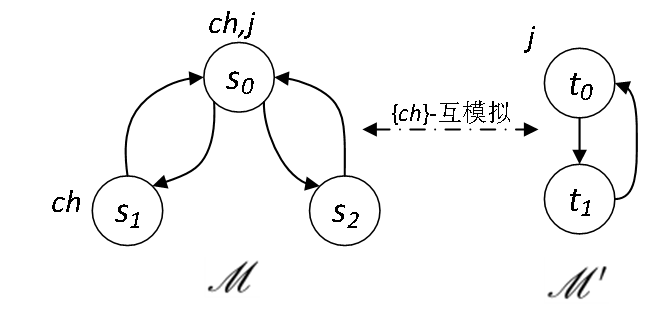
\includegraphics[scale=0.35]{figures/chvB3}
%%			\end{figure} 
%%		\end{columns}
%%	\end{block}
%%	\begin{proposition}[不变性]
%%		\label{pro:variB}
%%		令$\varphi$为$\mu$-公式、${\cal V}_1\subseteq {\cal V}$且$V\subseteq \Ha$。 若$(\Hm, s, v) \lrto_{\tuple{{\cal V}_1, V}} (\Hm', s', v')$且$\IR(\varphi,$ $ V \cup {\cal V}_1)$,则$(\Hm,s, v) \models \varphi$当且仅当$(\Hm',s', v') \models \varphi$。
%%	\end{proposition}
%%}
%%\only<5>{
%%	\begin{proposition} \label{pro:EqUnion}
%%		令${\cal V}_1, {\cal V}_2\subseteq {\cal V}$、$V, V_1 \subseteq \Ha$且$\Hm_i$为Kripke结构($i=1,2,3$),若$v_i: {\cal V}\rto 2^{S_i}$,则:
%%		\begin{enumerate} [(i)]
%%			\item $\lrto_{\tuple{{\cal V}_1,V}}$为赋值间的等价关系;
%%			\item 若$(\Hm_1, s_1,v_1) \lrto_{\tuple{{\cal V}_1,V}} (\Hm_2,s_2,v_2)$、${\cal V}_1 \subseteq {\cal V}_2$且$V \subseteq V_1$,\\
%%			则 $(\Hm_1, s_1, v_1) \lrto_{\tuple{{\cal V}_2,V_1}} (\Hm_2, s_2, v_2)$;
%%			\item 若$(\Hm_1, s_1, v_1) \lrto_{\tuple{{\cal V}_1,V}} (\Hm_2,s_2, v_2)$且$(\Hm_2,s_2, v_2) \lrto_{\tuple{{\cal V}_2,V_1}} (\Hm_3,s_3, v_3)$,\\
%%			则 $(\Hm_1,s_1,v_1) \lrto_{\tuple{{\cal V}_1 \cup {\cal V}_2, V \cup V_1}} (\Hm_3,s_3,v_3)$。
%%		\end{enumerate} 
%%	\end{proposition}
%%\begin{proposition}[不变性]
%%	\label{pro:variB}
%%	令$\varphi$为$\mu$-公式、${\cal V}_1\subseteq {\cal V}$且$V\subseteq \Ha$。 若$(\Hm, s, v) \lrto_{\tuple{{\cal V}_1, V}} (\Hm', s', v')$且$\IR(\varphi,$ $ V \cup {\cal V}_1)$,则$(\Hm,s, v) \models \varphi$当且仅当$(\Hm',s', v') \models \varphi$。
%%\end{proposition}
%%} 
%	}
%\end{frame}
%
%\subsection{$\mu$-演算遗忘理论}
%\begin{frame}
%	\frametitle{~$\mu$-演算遗忘理论——{\footnotesize 定义及相关性质}}
%	{\footnotesize
%%	\only<1>{
%	\begin{definition}[$\mu$-演算遗忘]\label{chapter06:def:V:forgetting}
%			令$V\subseteq\cal A$和 $\varphi$为$\mu$-公式。若$\Var(\psi) \cap V=\emptyset$且下面等式成立,则称
%			$\psi$是从$\varphi$中遗忘$V$后得到的结果:
%			\begin{equation*}
%				\Mod(\psi)=\{(\Hm,v) \mid \exists (\Hm',v') \in\Mod(\varphi)\ \hbox{且} (\Hm',v') \lrto_V (\Hm,v)\}\hbox{。}
%			\end{equation*}
%		\end{definition}\pause
%%	}
%%	\only<2>{
%		\begin{block}{与CTL共同性质}
%			表达性定理、分解性、同质性等。
%		\end{block}
%	
%		\begin{theorem}[存在性] \label{thm:exist}
%			给定原子命题 $q \in \cal A$和$\mu$-句子 $\varphi$,则存在一个$\mu$-句子 $\psi$使得 $\Var(\psi)\cap \{q\} = \emptyset$且 $\psi \equiv \Muforget(\varphi, \{q\})$。
%		\end{theorem}
%		\begin{proposition}[同质性]\label{chapter06:pro:mu:forget:2}
%			给定原子命题集$V\subseteq\cal A$和$\mu$-公式 $\varphi$,则: 
%			\begin{itemize}
%		%		\item[(i)] $\Muforget(\ALL\NEXT\varphi,V)\equiv \ALL\NEXT \Muforget(\varphi,V)$;
%		%		\item[(ii)] $\Muforget(\EXIST\NEXT\varphi,V)\equiv\EXIST\NEXT \Muforget(\varphi,V)$;
%			\item[(iii)] \textcolor{red} {如果$\nu X. \varphi$为$\mu$-句子,$\Muforget(\nu X. \varphi, V) \equiv \nu X. \Muforget(\varphi, V)$;
%				\item[(iv)] 如果$\mu X. \varphi$为$\mu$-句子,$\Muforget(\mu X. \varphi, V) \equiv \mu X. \Muforget(\varphi, V)$。}
%			\end{itemize}
%		\end{proposition}
%%	}
%	}
%\end{frame}
%
%\begin{frame}
%	\frametitle{~$\mu$-演算遗忘理论——{\footnotesize 不含不动点算子的子类}}
%	{\footnotesize
%	 \begin{block}{$\NEXT$-类}
%			不含有不定点操作的$\mu$-公式集,记为\textbf{$\NEXT$-类}。
%			通过等值式:
%			\begin{itemize}
%				\item $\ALL\NEXT \varphi_1 \wedge \ALL\NEXT \varphi_2 \equiv \ALL\NEXT (\varphi_1 \wedge \varphi_2)$;和
%				\item $\EXIST\NEXT \varphi_1 \vee \EXIST\NEXT \varphi_2 \equiv \EXIST\NEXT (\varphi_1 \vee \varphi_2)$;
%			\end{itemize}
%		可以将$\NEXT$-类中的任意公式转换为具有下面形式的公式的析取:
%			\begin{align}
%				\label{equ:form}
%				\varphi_0 \wedge \ALL\NEXT \varphi_1 \wedge \EXIST\NEXT \varphi_2 \wedge \dots \wedge \EXIST \NEXT \varphi_n\hbox{,}
%			\end{align}
%			其中$\varphi_0$是不含有时序算子的$\NEXT$-类中的公式,$\varphi_i$ ($1\leq i \leq n$)为$\NEXT$-类中的公式,且
%			任意$\varphi_i$ ($0\leq i \leq n$) 都有可能缺失。
%		\end{block} 
%	\begin{proposition}\label{pro:axexclass}
%		若$V\subseteq \Ha$为原子命题集、$\varphi$为$\NEXT$-类中的公式,则存在$\NEXT$-类中的公式$\psi$使得$\psi \equiv \Muforget(\varphi, V)$。
%	\end{proposition}
%%	\begin{block}{公式的度}
%%		给定$\NEXT$-类中的公式$\varphi$,公式$\varphi$的度(记为$degree(\varphi)$)定义如下:
%%		\begin{align*}
%%			& degree(X) = degree(p) = degree(\neg p) = 0,\\ %\hbox{ where } X\in {\cal V} \hbox{ and } p \in \Ha,\\
%%			& degree(\ALL\NEXT \psi) = degree(\psi) + 1, \\
%%			& degree(\EXIST\NEXT \psi) = degree(\psi) + 1, \\
%%			& degree(\psi_1 * \psi_2) = \max\{degree(\psi_1), degree(\psi_2)\},  
%%		\end{align*}
%%		其中$X\in {\cal V}$、$p \in \Ha$和$* \in \{\vee, \wedge\}$。
%%	\end{block}
%	%}
%%	\only<2>{
%%		\begin{lemma}\label{lem:geneq}
%%			令$V\subseteq \Ha$ 为原子命题集,$\varphi_0 \wedge \ALL\NEXT \varphi_1 \wedge \EXIST\NEXT \varphi_2 \wedge \dots \wedge \EXIST \NEXT \varphi_n$为具有形式 (\ref{equ:form})的可满足公式,则
%%			\begin{align*}
%%				\Muforget(\varphi_0 \wedge \ALL\NEXT \varphi_1 & \wedge \EXIST\NEXT \varphi_2 \wedge \dots \wedge \EXIST \NEXT \varphi_n,V) \\
%%				\equiv &\ \Muforget(\varphi_0, V) \wedge \Muforget(\ALL\NEXT \varphi_1, V) \wedge \bigwedge_{2\leq i\leq n}  \Muforget(\EXIST\NEXT(\varphi_i \wedge \varphi_1), V)\\
%%				\equiv &\  \Muforget(\varphi_0, V) \wedge \ALL\NEXT\Muforget(\varphi_1, V) \wedge \bigwedge_{2\leq i\leq n} \EXIST\NEXT \Muforget(\varphi_i \wedge \varphi_1, V).
%%			\end{align*}
%%		\end{lemma}
%%	\begin{proposition}\label{pro:axexclass}
%%		若$V\subseteq \Ha$为原子命题集、$\varphi$为$\NEXT$-类中的公式,则存在$\NEXT$-类中的公式$\psi$使得$\psi \equiv \Muforget(\varphi, V)$。
%%	\end{proposition}
%%	} 
%	}
%\end{frame}
%
%%\begin{frame} 
%%	\frametitle{~$\mu$-演算遗忘理论——{\footnotesize 不含不动点算子的子类}}
%%{\tiny	\begin{example}
%%		\label{exp:x-class}
%%		令$\varphi_1 = X \wedge p$、$\varphi_2 = \ALL\NEXT(c \wedge \EXIST\NEXT d) \wedge \ALL\NEXT e$、$\varphi_3 = \EXIST\NEXT \neg d \wedge (\EXIST\NEXT \neg p \vee \EXIST\NEXT p)$、$\varphi = \varphi_1 \wedge \varphi_2 \wedge \varphi_3$且$V = \{e,d\}$,其中$X \in {\cal V}$且$p, c, d, e$为原子命题。 
%%		\begin{columns}
%%			\column{0.5\textwidth}
%%			
%%		如下计算公式$\varphi$的度:
%%		
%%		\begin{align*}
%%			degree(\varphi) &  =  \max\{degree(\varphi_1), degree(\varphi_2 \wedge \varphi_3)\}\\
%%			& = \max\{0, \max\{degree(\varphi_2), degree(\varphi_3)\}\\
%%			& = 2,\\
%%			degree(\varphi_1) & = 0,\\
%%			degree(\varphi_2) & = \max\{degree(\ALL\NEXT(c \wedge \EXIST\NEXT d)), degree(\ALL\NEXT e)\}\\
%%			& =\max\{\max\{0, 1\} + 1, 1\}\\
%%			& = 2,\\
%%			degree(\varphi_3) & = \max\{degree(\EXIST\NEXT \neg d), degree(\EXIST\NEXT \neg p \vee \EXIST\NEXT p)\}\\
%%			& = \max\{1, \max\{1,1\}\}\\
%%			& = 1.
%%		\end{align*}
%%		
%%	\column{0.5\textwidth}
%%	此外,公式$\varphi$可如下转换为具有形式(\ref{equ:form})的公式的析取:
%%	\begin{align*}
%%		\varphi & = \varphi_1 \wedge \varphi_2 \wedge \varphi_3\\
%%		& \equiv X \wedge p \wedge \ALL\NEXT(c \wedge e \wedge \EXIST\NEXT d) \wedge \EXIST\NEXT \neg d \wedge (\EXIST\NEXT \neg p \vee \EXIST\NEXT p)\\
%%		& \equiv (X \wedge p \wedge \ALL\NEXT(c \wedge e \wedge \EXIST\NEXT d) \wedge \EXIST\NEXT \neg d \wedge \EXIST\NEXT \neg p) \vee\\
%%		& \quad\ (X \wedge p \wedge \ALL\NEXT(c \wedge e \wedge \EXIST\NEXT d) \wedge \EXIST\NEXT \neg d \wedge \EXIST\NEXT  p).
%%	\end{align*}
%%		则从$\varphi$中遗忘$V$的结果为:
%%		\begin{align*}
%%			\Muforget(\varphi,V) & \equiv \Muforget(X \wedge p \wedge \ALL\NEXT(c \wedge e \wedge \EXIST\NEXT d) \wedge \EXIST\NEXT \neg d \wedge \EXIST\NEXT \neg p, V) \vee \\
%%			& \qquad \Muforget(X \wedge p \wedge \ALL\NEXT(c \wedge e \wedge \EXIST\NEXT d) \wedge \EXIST\NEXT \neg d \wedge \EXIST\NEXT  p,V) \\
%%			 \equiv (X \wedge p & \wedge \ALL\NEXT\Muforget(c \wedge e \wedge \EXIST\NEXT d, V) \wedge\\
%%			&  \EXIST\NEXT\Muforget(\neg d \wedge c \wedge e \wedge \EXIST\NEXT d, V) \wedge  \EXIST\NEXT\Muforget(\neg p \wedge c \wedge e \wedge \EXIST\NEXT d, V) )\vee \\
%%			&  (X \wedge p \wedge \ALL\NEXT\Muforget(c \wedge e \wedge \EXIST\NEXT d, V) \wedge\\
%%			&  \EXIST\NEXT\Muforget(\neg d \wedge c \wedge e \wedge \EXIST\NEXT d, V) \wedge  \EXIST\NEXT\Muforget( p \wedge c \wedge e \wedge \EXIST\NEXT d, V)) \\
%%		 \equiv 	(X \wedge p & \wedge \ALL\NEXT c \wedge \EXIST\NEXT c \wedge \EXIST\NEXT (\neg p \wedge c)) \vee 
%%			(X \wedge p \wedge \ALL\NEXT c \wedge \EXIST\NEXT c \wedge \EXIST\NEXT (p \wedge c)) \\
%%			 \equiv  X \wedge p & \wedge \ALL\NEXT c \wedge \EXIST\NEXT c \wedge (\EXIST\NEXT (\neg p \wedge c) \vee \EXIST\NEXT (p \wedge c)).
%%		\end{align*}
%%	\end{columns}
%%	\end{example}
%%}
%%\end{frame}
%
%\begin{frame} 
%	\frametitle{~$\mu$-演算遗忘理论——{\footnotesize 复杂性结果}}
%	{\footnotesize
%%	\only<1>{
%		\begin{proposition}[模型检测]\label{chapter06:pro:MC}
%		给定一个有限的 Kripke 结构  $\Hm$、一个 $\mu$-句子 $\varphi$和原子命题集 $V\subseteq \Ha$。有:
%		\begin{itemize}
%			\item[(i)] 判定 $\Hm \models^? \Muforget(\varphi, V)$在$\textsc{Exptime}$中;
%			\item[(ii)] 若 $\varphi$是一个析取 $\mu$-公式,则判定 $\Hm \models^? \Muforget(\varphi, V)$在 \textsc{NP}$\cap$co-\textsc{NP}中。
%		\end{itemize}
%	\end{proposition}
%\begin{theorem}[Entailment]
%	\label{thm:Ent}
%	给定$\mu$-句子$\varphi$和 $\psi$,$V$为原子命题集,则:
%	\begin{itemize}
%		\item[(i)] 判定 $\Muforget(\varphi, V ) \models^? \psi$是$\textsc{Exptime}$-完全的,
%		\item[(ii)] 判定 $\psi \models^? \Muforget(\varphi, V)$在$\textsc{Exptime}$里,
%		\item[(iii)] 判定 $\Muforget(\varphi, V) \models^? \Muforget(\psi, V)$在$\textsc{Exptime}$里。
%	\end{itemize}
%\end{theorem}
%%}
%%\only<2>{\begin{theorem}[Entailment]
%%	\label{thm:Ent}
%%	给定$\mu$-句子$\varphi$和 $\psi$,$V$为原子命题集,则:
%%	\begin{itemize}
%%		\item[(i)] 判定 $\Muforget(\varphi, V ) \models^? \psi$是$\textsc{Exptime}$-完全的,
%%		\item[(ii)] 判定 $\psi \models^? \Muforget(\varphi, V)$在$\textsc{Exptime}$里,
%%		\item[(iii)] 判定 $\Muforget(\varphi, V) \models^? \Muforget(\psi, V)$在$\textsc{Exptime}$里。
%%	\end{itemize}
%%\end{theorem}
%%
%%\begin{corollary}\label{chapter06:cor:equiv}
%%	给定$\mu$-句子$\varphi$和 $\psi$,$V$为原子命题集。则下面的判定问题在$\textsc{Exptime}$里。
%%	\begin{itemize}
%%		\item[(i)] 判定 $\psi \equiv^?\Muforget(\varphi, V)$,
%%		\item[(ii)] 判定 $\Muforget(\varphi, V) \equiv^? \varphi$,
%%		\item[(iii)] 判定 $\Muforget(\varphi, V) \equiv^? \Muforget(\psi, V)$。
%%	\end{itemize}
%%\end{corollary}}
%}
%\end{frame}

\section{研究内容(二)遗忘理论在反应式系统中的应用}
%\subsection{研究内容(二)遗忘理论在反应式系统中的应用}
\begin{frame}
	\frametitle{~研究内容(二)遗忘理论在反应式系统中的应用}
	{\footnotesize
	\begin{columns}
		\column{0.5\textwidth}
		\begin{itemize}
			\item 反应式系统被表示成Kripke结构;
			\item 初始Kripke结构的特征公式看作CTL公式——${\cal F}_{\Ha}(\Hm)$;
		\end{itemize}
	\column{0.5\textwidth}
	\begin{figure}
		\centering
	%	\tiny
		\begin{tikzpicture}[scale=0.8]
			\tikzstyle{every node}=[font=\small,scale=0.8]
			\node[blueCircle] (s0) at(0,1) {{\tiny 就绪}};
			\node[blueCircle1] (s1) at(0.8,-0.2) {{\tiny 执行}};
			\node[redCircle] (s2) at(-0.8,-0.2) {{\tiny 阻塞}};  
			\path (s1) edge[->,bend right=45] (s0);
			\path (s0) edge[->,bend left=-45] (s1);
			\path (s1) edge[->,bend right=-45] (s2);
			\path (s2) edge[->,bend right=-45] (s0); 
			\node at(0,-0.5) {{\tiny $I/O$请求}};
			\node at(-1,0.5) {{\tiny $I/O$完成}};
			\node at(0.7,0.5) {{\tiny 时间片完}};
			\node at(-0.2,0.3) {{\tiny 进程调度}};
			%	\node at(0,-1.5) {${\cal K}_2$}; 
		\end{tikzpicture}
		\caption{{\scriptsize 进程的三种基本状态及其转换}}
	\end{figure}
%		 \begin{figure}
%		 	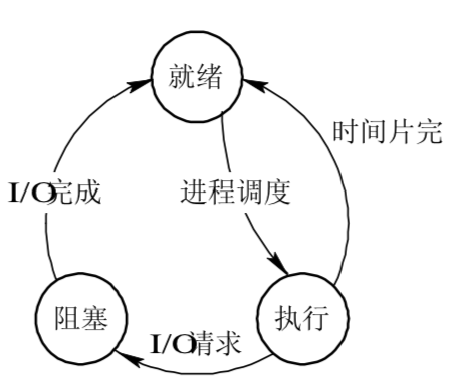
\includegraphics[scale=0.28]{figures/processState}
%		 	\caption{{\scriptsize 进程的三种基本状态及其转换}}
%		 \end{figure}
	\end{columns}
} 
\begin{figure} 
	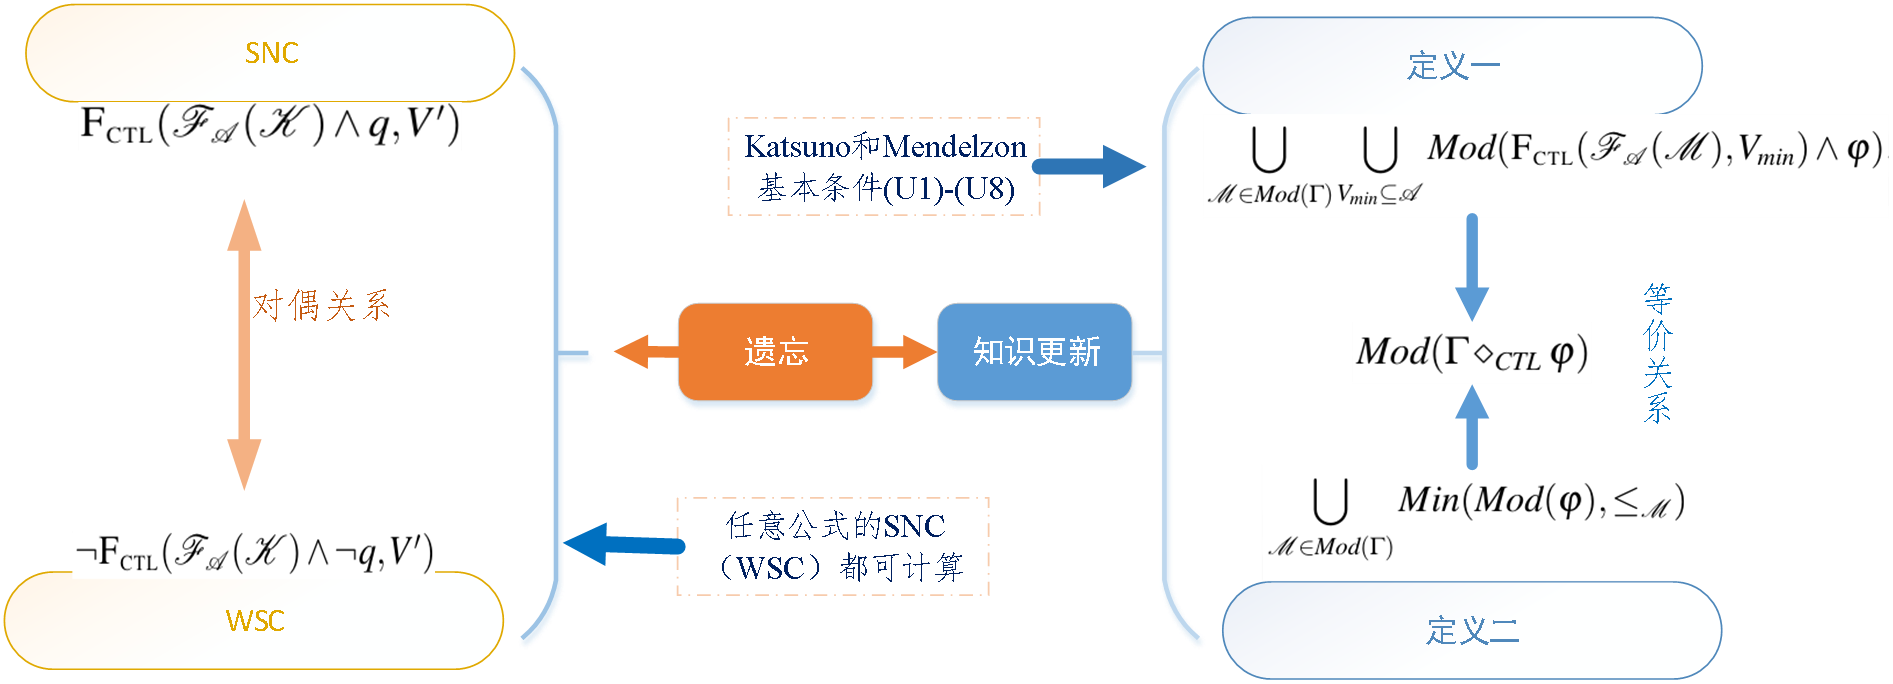
\includegraphics[scale=0.27]{figures/sncAndWsc}
	%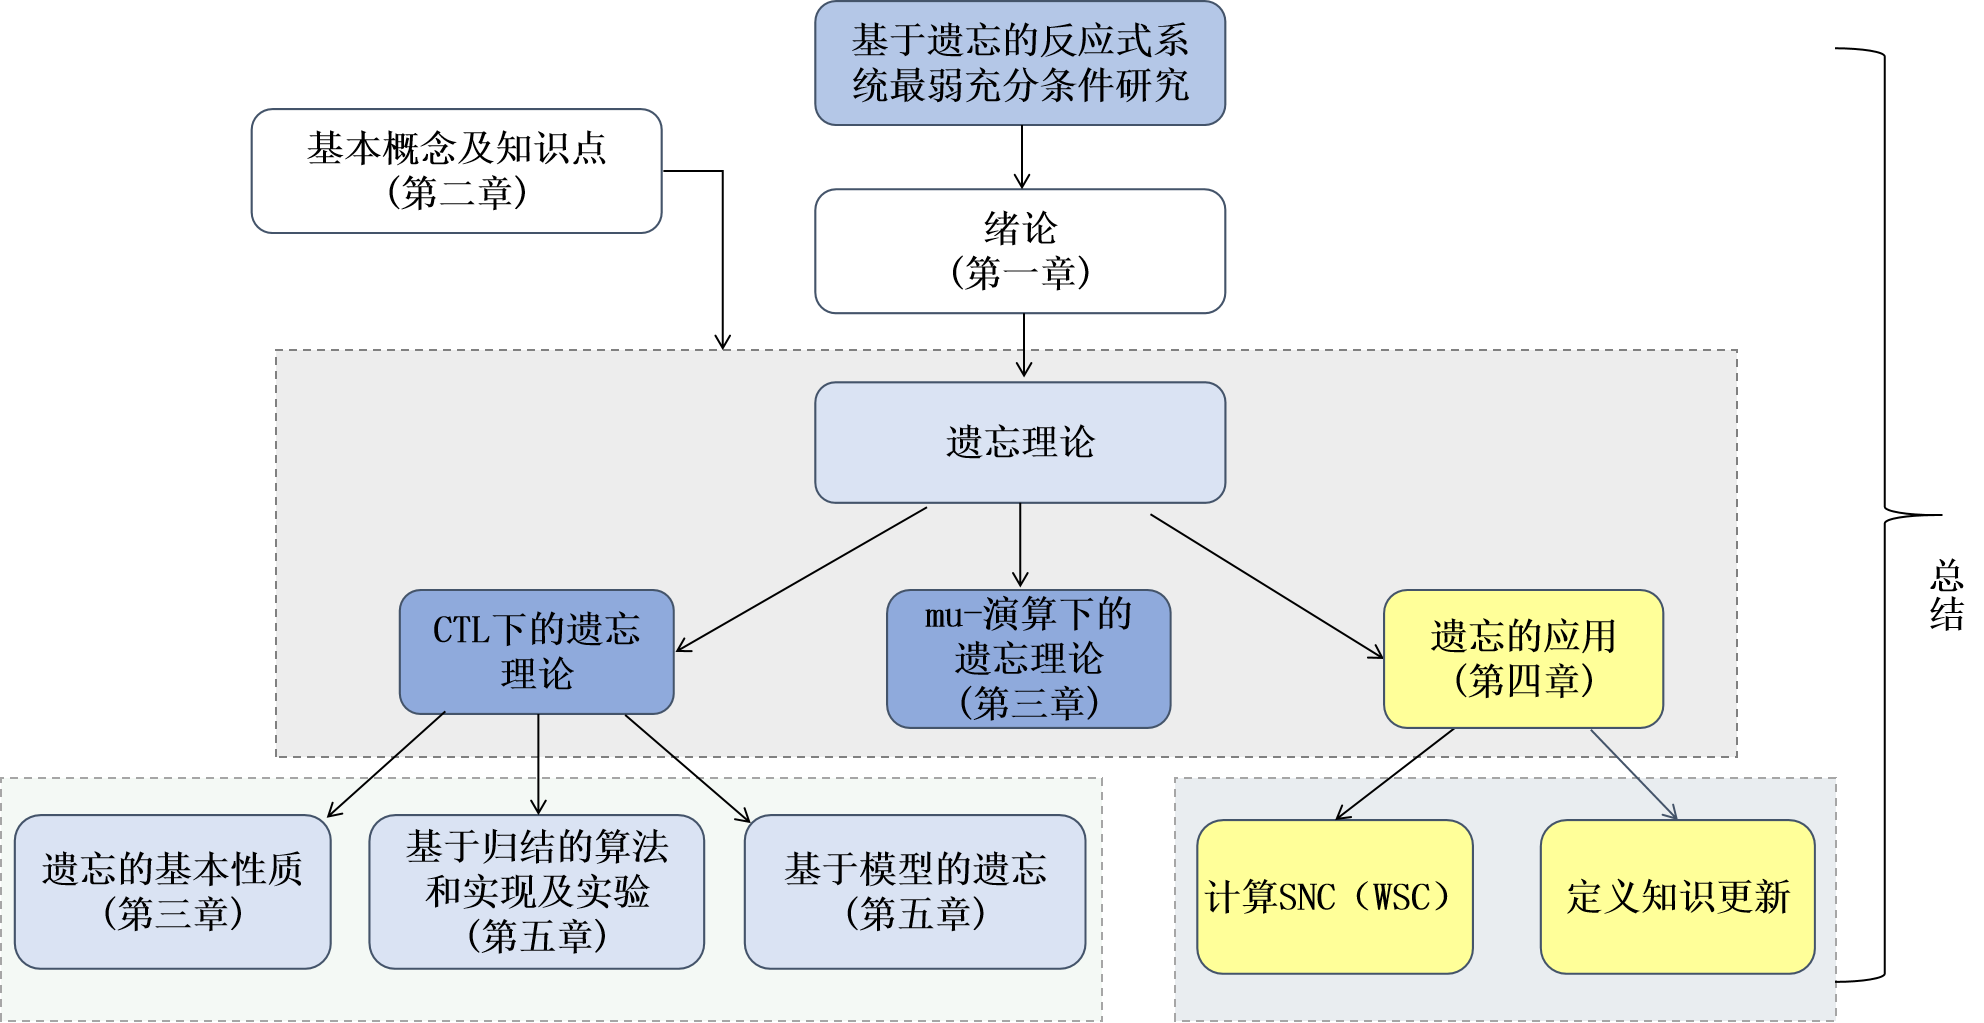
\includegraphics[scale=0.27]{figures/applicationF4}
%	\caption{进程的三种基本状态及其转换}
\end{figure} 
\end{frame}


\begin{frame}
\frametitle{~研究内容(二)遗忘理论在反应式系统中的应用}
{\footnotesize
	\begin{columns}
		\column{0.5\textwidth}
		\begin{itemize}
			\item 反应式系统被表示成Kripke结构;
			\item 初始Kripke结构的特征公式看作CTL公式——${\cal F}_{\Ha}(\Hm)$;
		\end{itemize}
		\column{0.5\textwidth}
		\begin{figure}
			\centering
			%	\tiny
			\begin{tikzpicture}[scale=0.8]
				\tikzstyle{every node}=[font=\small,scale=0.8]
				\node[blueCircle] (s0) at(0,1) {{\tiny 就绪}};
				\node[blueCircle1] (s1) at(0.8,-0.2) {{\tiny 执行}};
				\node[redCircle] (s2) at(-0.8,-0.2) {{\tiny 阻塞}};  
				\path (s1) edge[->,bend right=45] (s0);
				\path (s0) edge[->,bend left=-45] (s1);
				\path (s1) edge[->,bend right=-45] (s2);
				\path (s2) edge[->,bend right=-45] (s0); 
				\node at(0,-0.5) {{\tiny $I/O$请求}};
				\node at(-1,0.5) {{\tiny $I/O$完成}};
				\node at(0.7,0.5) {{\tiny 时间片完}};
				\node at(-0.2,0.3) {{\tiny 进程调度}};
				%	\node at(0,-1.5) {${\cal K}_2$}; 
			\end{tikzpicture}
			\caption{{\scriptsize 进程的三种基本状态及其转换}}
		\end{figure}
		%		 \begin{figure}
		%		 	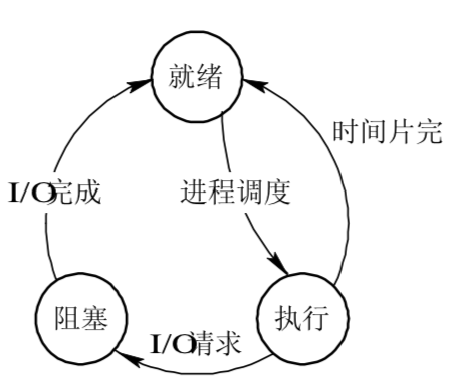
\includegraphics[scale=0.28]{figures/processState}
		%		 	\caption{{\scriptsize 进程的三种基本状态及其转换}}
		%		 \end{figure}
	\end{columns}
} 
\begin{figure} 
	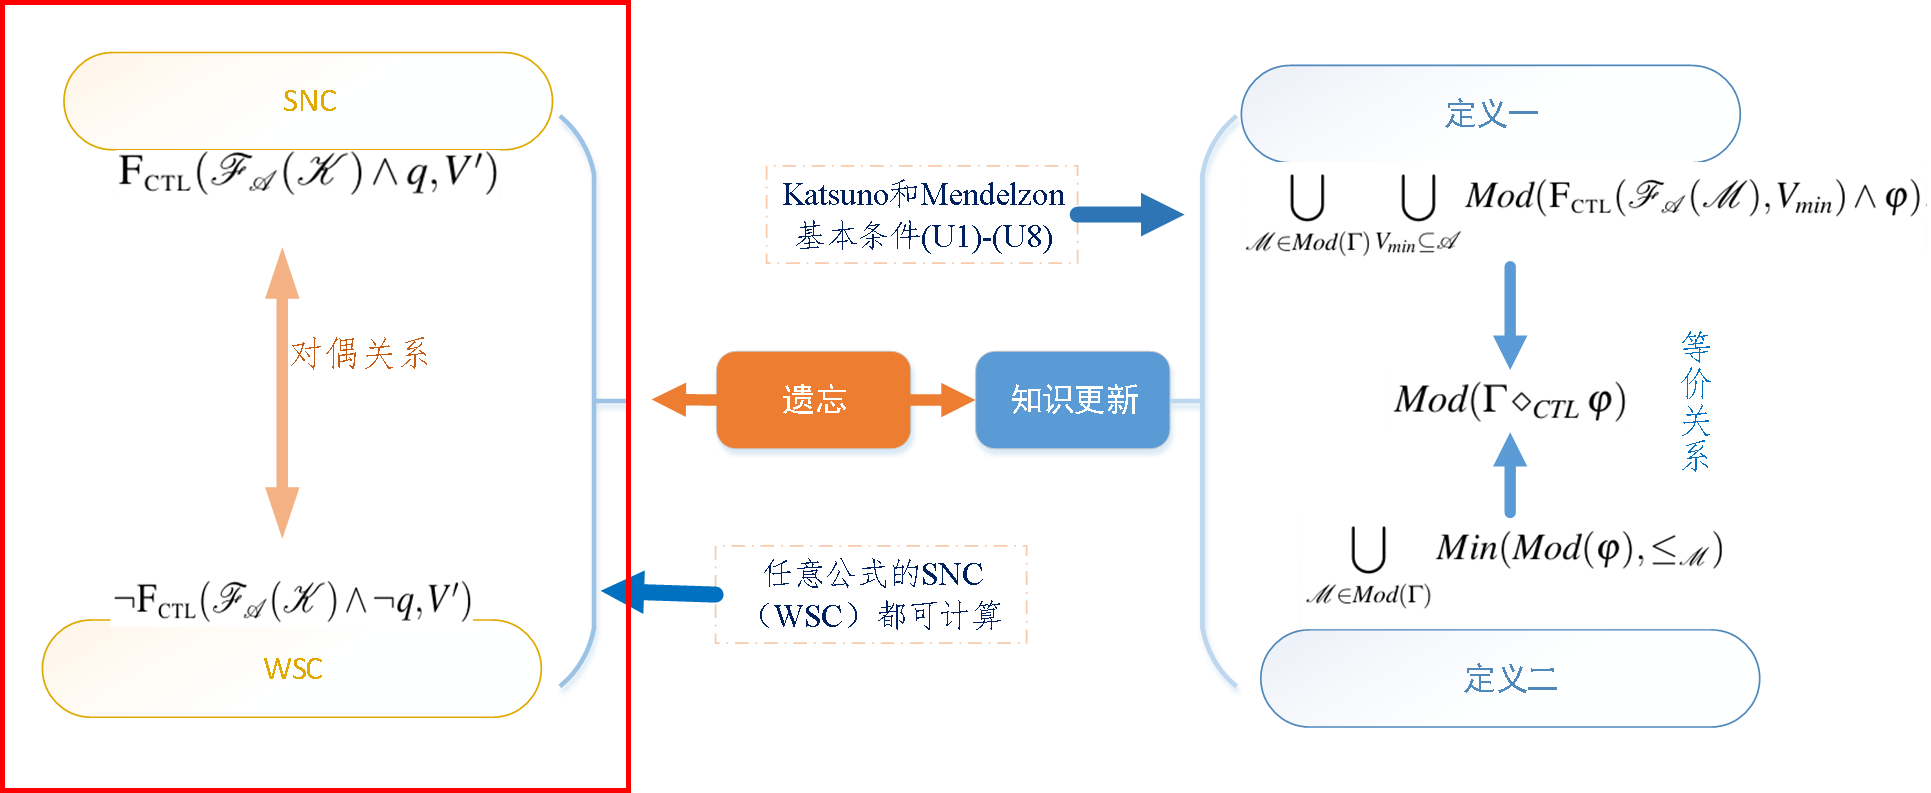
\includegraphics[scale=0.27]{figures/sncAndWsc1}
	%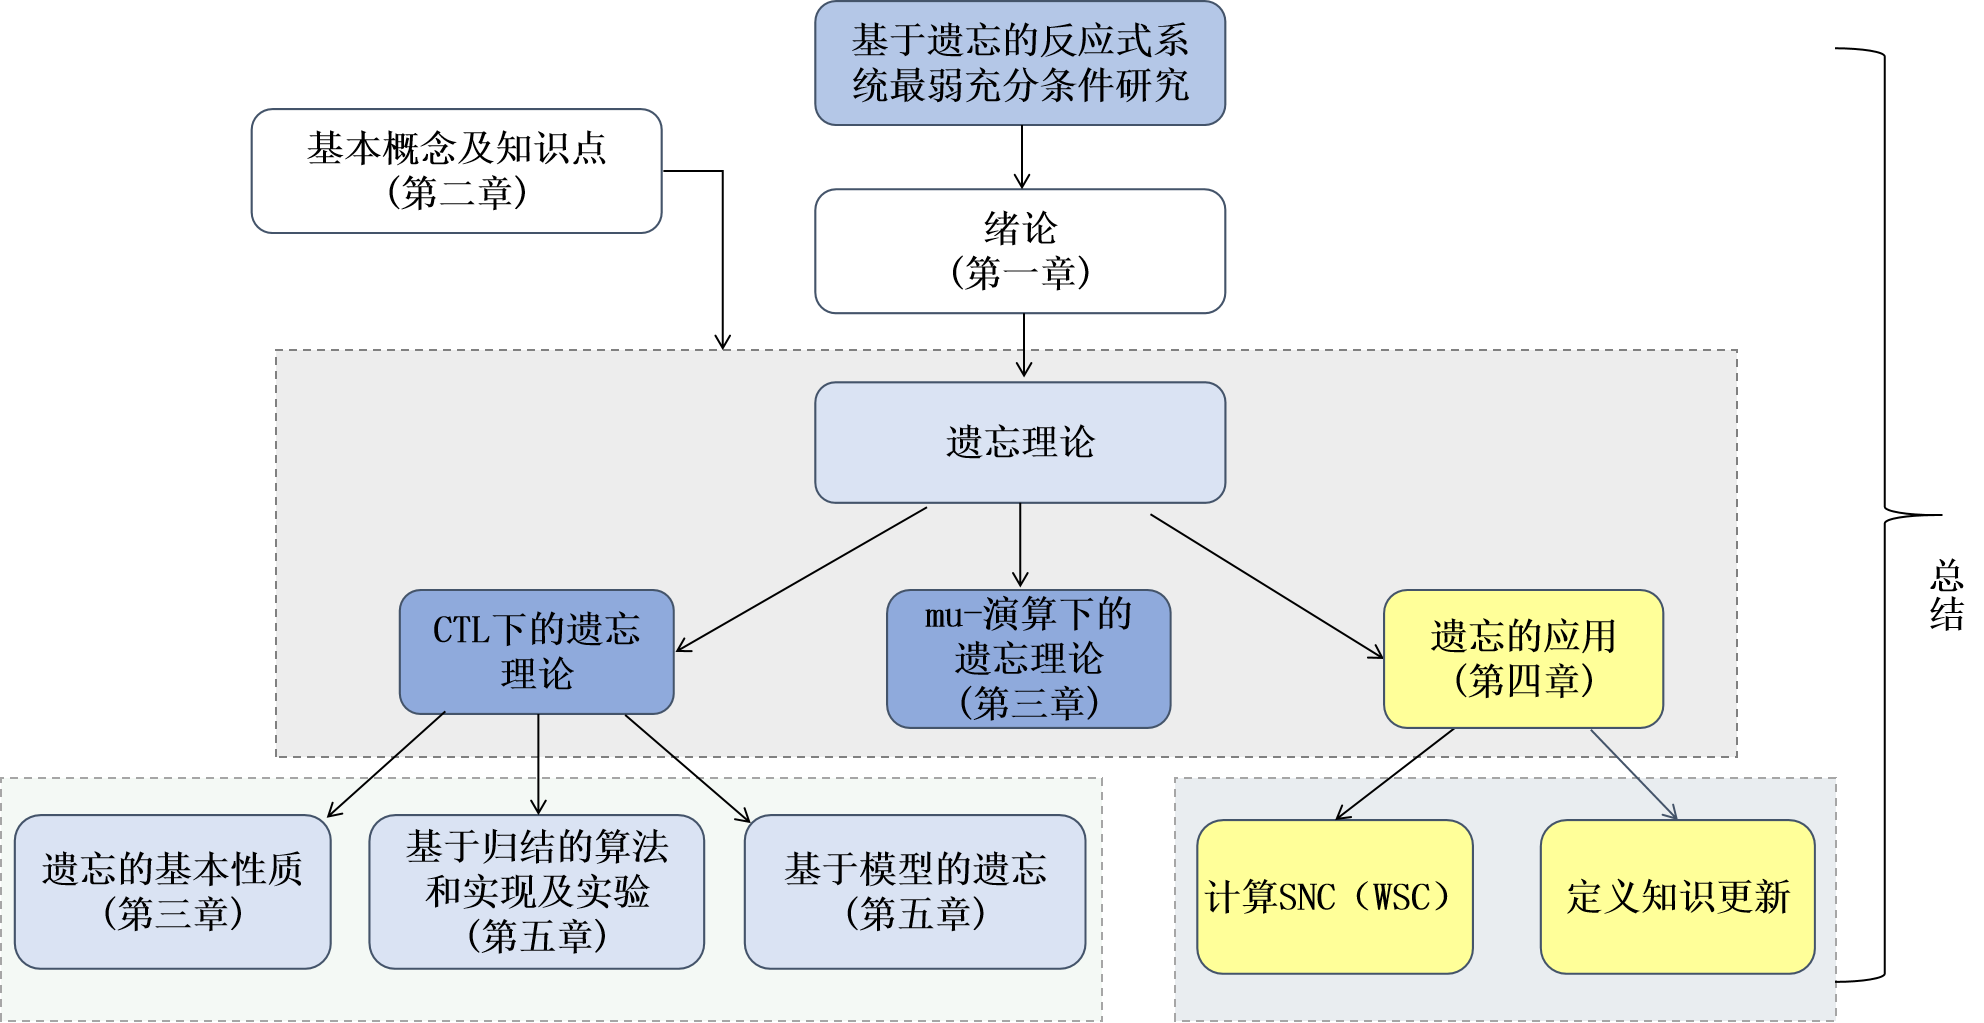
\includegraphics[scale=0.27]{figures/applicationF4}
	%	\caption{进程的三种基本状态及其转换}
\end{figure} 
\end{frame}

\begin{frame}
	\frametitle{~研究内容(二)遗忘理论在反应式系统中的应用}
	{\footnotesize
		\begin{columns}
			\column{0.5\textwidth}
			\begin{itemize}
				\item 反应式系统被表示成Kripke结构;
				\item 初始Kripke结构的特征公式看作CTL公式——${\cal F}_{\Ha}(\Hm)$;
			\end{itemize}
			\column{0.5\textwidth}
			\begin{figure}
				\centering
				%	\tiny
				\begin{tikzpicture}[scale=0.8]
					\tikzstyle{every node}=[font=\small,scale=0.8]
					\node[blueCircle] (s0) at(0,1) {{\tiny 就绪}};
					\node[blueCircle1] (s1) at(0.8,-0.2) {{\tiny 执行}};
					\node[redCircle] (s2) at(-0.8,-0.2) {{\tiny 阻塞}};  
					\path (s1) edge[->,bend right=45] (s0);
					\path (s0) edge[->,bend left=-45] (s1);
					\path (s1) edge[->,bend right=-45] (s2);
					\path (s2) edge[->,bend right=-45] (s0); 
					\node at(0,-0.5) {{\tiny $I/O$请求}};
					\node at(-1,0.5) {{\tiny $I/O$完成}};
					\node at(0.7,0.5) {{\tiny 时间片完}};
					\node at(-0.2,0.3) {{\tiny 进程调度}};
					%	\node at(0,-1.5) {${\cal K}_2$}; 
				\end{tikzpicture}
				\caption{{\scriptsize 进程的三种基本状态及其转换}}
			\end{figure}
			%		 \begin{figure}
			%		 	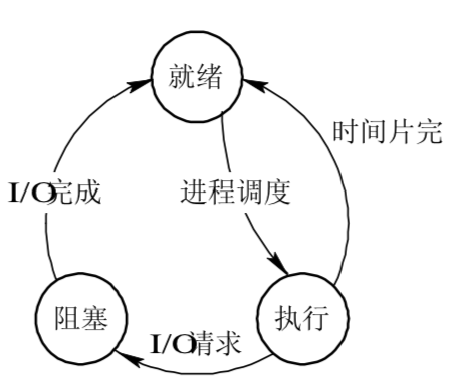
\includegraphics[scale=0.28]{figures/processState}
			%		 	\caption{{\scriptsize 进程的三种基本状态及其转换}}
			%		 \end{figure}
		\end{columns}
	} 
	\begin{figure} 
		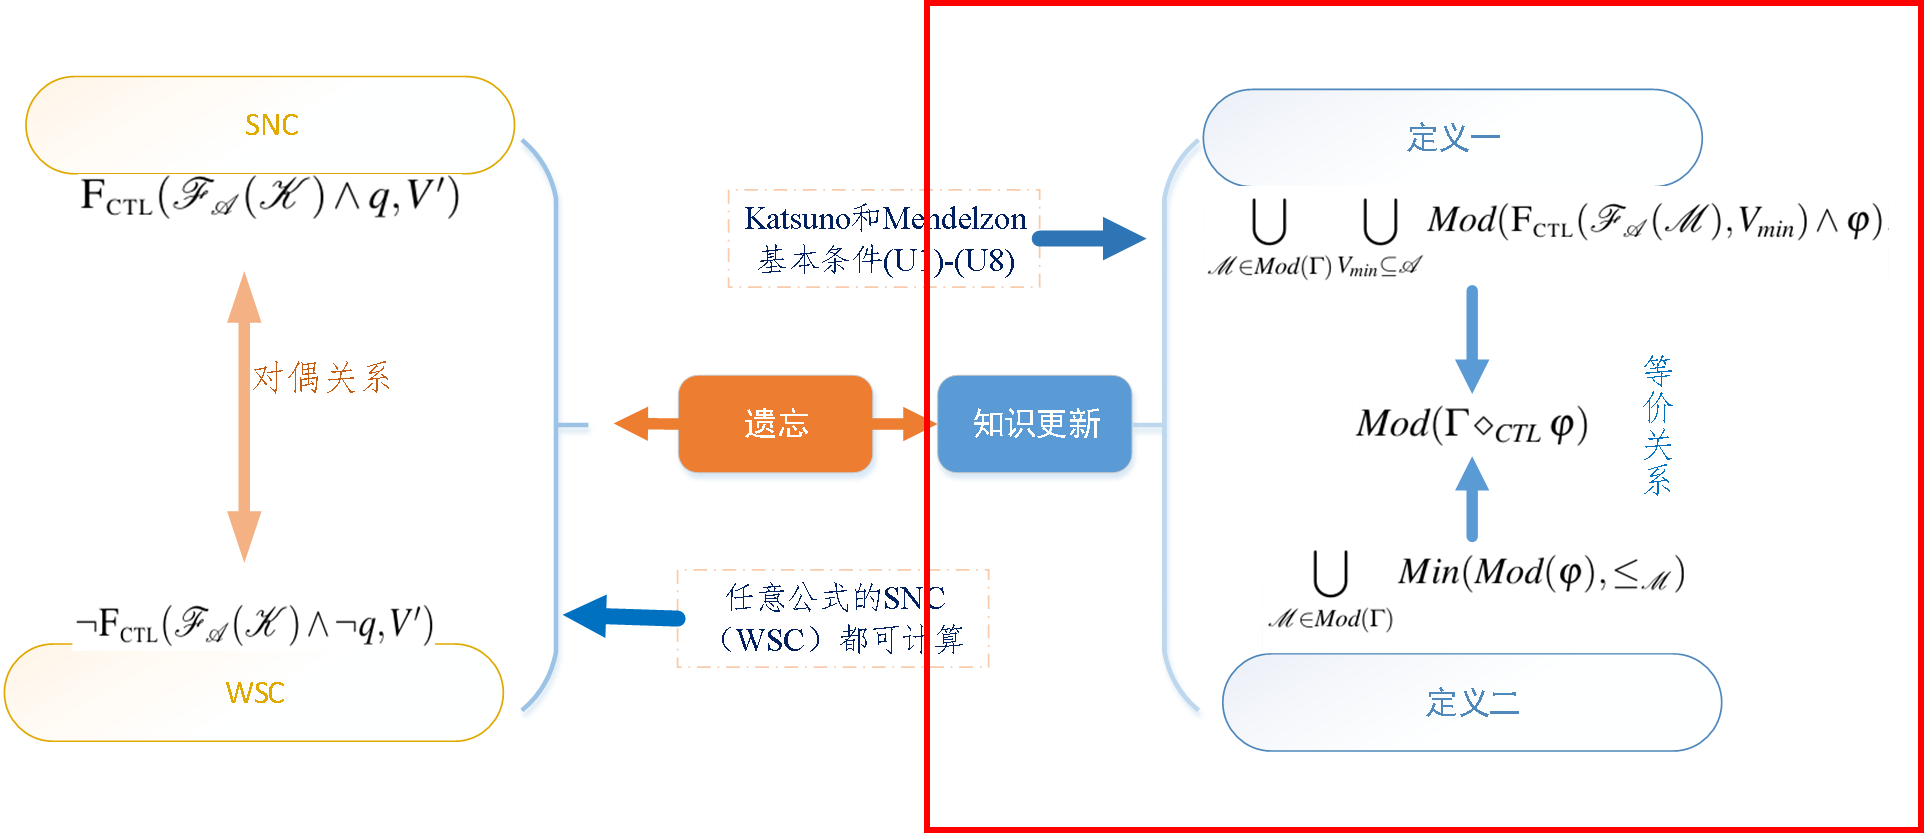
\includegraphics[scale=0.27]{figures/sncAndWsc2}
		%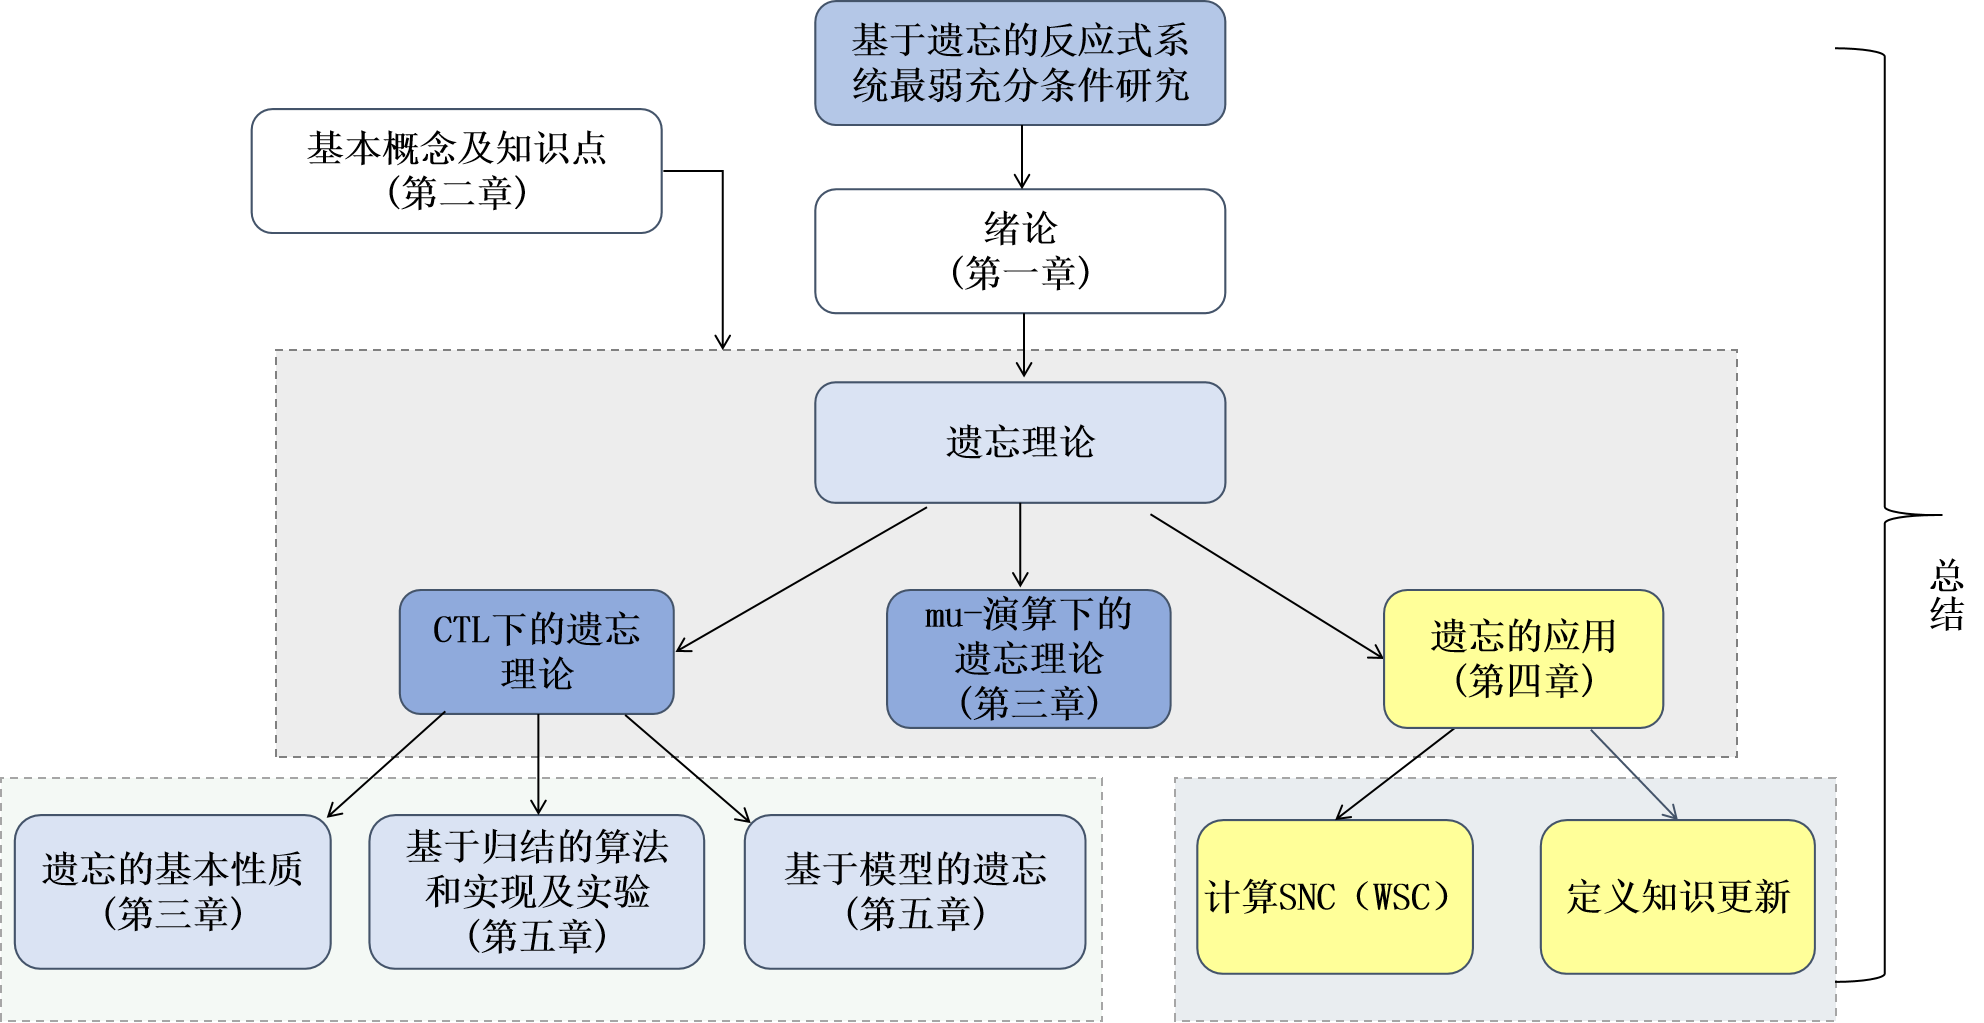
\includegraphics[scale=0.27]{figures/applicationF4}
		%	\caption{进程的三种基本状态及其转换}
	\end{figure}
	\pause
	\textcolor{red}{\[\hbox{从而为系统正确性和系统更新提供了理论依据!}\]}
\end{frame}

%
%\subsection{研究内容(二)最弱充分条件}
%\begin{frame}
%	\frametitle{~研究内容(二)最弱充分条件——{\footnotesize 定义}}
%	{\footnotesize
%		\begin{definition}[充分和必要条件]\label{def:NC:SC}
%			给定两个公式$\varphi$和$\psi$,$V \subseteq \Var(\varphi)$,$q\in\Var(\varphi)- V$
%			和$\Var(\psi)$ $\subseteq V$。
%			\begin{itemize}
%				\item 若$\varphi \models q \rto \psi$,则称$\psi$是$q$在$V$和$\varphi$上的{\em 必要条件(necessary condition,NC)};
%				\item 若$\varphi \models \psi\rto q$,则称$\psi$是$q$在$V$和$\varphi$上的{\em 充分条件(sufficient condition,SC)};
%				\item 若$\psi$是$q$在$V$和$\varphi$上的必要条件,且对于任意$q$在$V$和$\varphi$上的必要条件$\psi'$,都有$\varphi\models\psi\rto\psi'$,则称$\psi$是$q$在$V$和$\varphi$上的{\em 最强必要条件(strongest necessary condition,SNC)};
%				\item 若$\psi$是$q$在$V$和$\varphi$上的充分条件,且对于任意$q$在$V$和$\varphi$上的充分条件$\psi'$,都有$\varphi\models\psi'\rto\psi$,则称$\psi$是$q$在$V$和$\varphi$上的{\em 最弱充分条件(weakest sufficient condition, WSC)}。
%			\end{itemize}
%		\end{definition}
%		\begin{theorem}\label{thm:SNC:WSC:forget}
%		给定公式$\varphi$、原子命题集$V\subseteq\Var(\varphi)$和原子命题$q\in\Var(\varphi)- V$。
%		\begin{itemize}
%			\item[(i)] $\CTLforget (\varphi \land q$, $(\Var(\varphi) \cup \{q\}) - V)$是$q$在$V$和$\varphi$上的SNC;
%			\item[(ii)]  $\neg\CTLforget (\varphi \land \neg q$, $(\Var(\varphi) \cup \{q\}) - V)$是$q$在$V$和$\varphi$上的WSC。
%		\end{itemize}
%	\end{theorem}
%%	{\tiny \begin{block}{{\scriptsize 小贴士}}
%%		\begin{itemize}
%%			\item WSC和SNC是一对对偶概念;
%%			\item 任意公式的WSC(SNC)能转换成原子命题的WSC(SNC)来计算。
%%		\end{itemize}
%%	\end{block}}
%	}
%\end{frame}
%%\begin{frame}
%%	\frametitle{~研究内容(二)最弱充分条件——{\footnotesize 相关性质}}
%%	{\footnotesize
%%%	\only<1>{\begin{proposition}[对偶性]\label{dual}
%%%			令$V$、$q$、$\varphi$和$\psi$为定义\ref{def:NC:SC}出现的符号。
%%%			则$\psi$是$q$在$V$和$\varphi$上的SNC(WSC)当且仅当$\neg \psi$是$\neg q$在$V$和$\varphi$上的WSC(SNC)。
%%%		\end{proposition}
%%%		\begin{proposition}\label{formulaNS_to_p}
%%%			给定公式$\Gamma$和$\alpha$, $V \subseteq \Var(\alpha) \cup \Var(\Gamma)$,$q$是不出现在$\Gamma$和$\alpha$中的原子命题。
%%%			$\varphi$是集合$V$上的公式,则$\varphi$是$\alpha$在$V$和$\Gamma$上的SNC(WSC) 当且仅当$\varphi$是$q$在$V$和$\Gamma'$上的SNC(WSC),其中$\Gamma' = \Gamma \cup \{q \lrto \alpha\}$。
%%%		\end{proposition}
%%%	}
%%%	\only<2>{
%%		\begin{theorem}\label{thm:SNC:WSC:forget}
%%		给定公式$\varphi$、原子命题集$V\subseteq\Var(\varphi)$和原子命题$q\in\Var(\varphi)- V$。
%%		\begin{itemize}
%%			\item[(i)] $\CTLforget (\varphi \land q$, $(\Var(\varphi) \cup \{q\}) - V)$是$q$在$V$和$\varphi$上的SNC;
%%			\item[(ii)]  $\neg\CTLforget (\varphi \land \neg q$, $(\Var(\varphi) \cup \{q\}) - V)$是$q$在$V$和$\varphi$上的WSC。
%%		\end{itemize}
%%	\end{theorem}
%%	\begin{example}[例~\ref{car_manufacturing}的延续]
%%		\label{exam:SNCandWSC}
%%		令$\Ha=\{d,se,sp,s\}$和$V=\{d,se\}$,求$s$在$V$和初始结构${\cal K} = (\Hm,s_0)$ 上的WSC,其中$\Hm$为例~\ref{car_manufacturing}中初始状态为$s_0$的汽车制造企业模型结构。
%%		
%%		由上面的定理可知,$s$在$V$和初始结构${\cal K} = (\Hm,s_0)$上的WSC为$\neg \CTLforget({\cal F}_{\Ha}({\cal K}) \wedge \neg s, \{s\}$ $\cup \{sp\})$。
%%		
%%		由于涉及到后文中遗忘的计算方法,\fbox{本例的详细计算过程放到后面}。
%%	\end{example}
%%%}
%%	}
%%\end{frame}
%
%\subsection{研究内容(二)知识更新}
%\begin{frame}
%	\frametitle{~研究内容(二)知识更新——{\footnotesize 定义 1}}
%	{\footnotesize
%		\begin{block}{约定}
%			\begin{itemize}
%				\item 本小节假设所有初始结构都是有限的,即:状态来源于有限状态空间且$\Ha$为有限原子命题集;
%				\item 任意$\Ha$上的有限初始结构$\Hm$(为了简化符号,用初始Kripke结构$\Hm$代替初始结构$(\Hm,s_0)$)都能用一个$\CTL$公式——\fbox{特征公式${\cal F}_{\Ha}(\Hm)$}来表示;
%				\item 给定公式$\varphi$和$\psi$,$V_{min}\subseteq \Ha$为使得$\CTLforget(\varphi, V_{min}) \wedge \psi$可满足的极小子集。
%				\item 记
%				$$\bigcup_{V_{min}\subseteq \Ha} \Mod(\CTLforget({\cal F}_{\Ha}(\Hm), V_{min}) \wedge \psi)$$  
%				为所有$\CTLforget({\cal F}_{\Ha}(\Hm), V_{min}) \wedge \psi$的模型集合的并集。
%			\end{itemize}
%		\end{block}
%	
%	\begin{definition}\label{def:KU}
%		给定公式$\Gamma$和$\varphi$。知识更新操作$\diamond_{\CTL}$定义如下:
%		\[
%		\Mod(\Gamma \diamond_{\CTL} \varphi) = \bigcup_{\Hm \in \Mod(\Gamma)} \bigcup_{V_{min}\subseteq \Ha} \Mod(\CTLforget({\cal F}_{\Ha}(\Hm), V_{min}) \wedge \varphi),
%		\]
%		其中,${\cal F}_{\Ha}(\Hm)$是$\Hm$在$\Ha$上的特征公式,$V_{min} \subseteq \Ha$是使得$\CTLforget({\cal F}_{\Ha}(\Hm), V_{min})$可满足的极小子集。
%	\end{definition}
%	}
%\end{frame}
%
%\begin{frame}
%	\frametitle{~研究内容(二)知识更新——{\footnotesize 定义 2及相关性质}}
%	{\footnotesize
%		\begin{definition}\label{def:closer}
%			给定三个有限初始结构$\Hm$、$\Hm_1$和$\Hm_2$,$\Hm_1$比$\Hm_2$更接近$\Hm$(记为$\Hm_1 \leq_{\Hm} \Hm_2$),当且仅当对任意$V_2 \subseteq \Ha$,若$\Hm_2 \lrto_{V_2} \Hm$,则存在$V_1 \subseteq V_2$使得$\Hm_1 \lrto_{V_1} \Hm$。
%			$\Hm_1 <_{\Hm} \Hm_2$当且仅当$\Hm_1 \leq_{\Hm} \Hm_2$且$\Hm_2 \not \leq_{\Hm} \Hm_1$。
%		\end{definition}
%	
%	\only<1>{\begin{example}
%	%	令$\Hm= (S, R, L, r)$、$\Hm_1 = (S_1, R_1, L_1, r_1)$、$\Hm_2 = (S_2, R_2, L_2, r_2)$为三个初始结构(如图~\ref{fig:partialo}),其中$S = S_1 = S_2 = \{s_0, s_1\}$,$r=r_1=r_2= s_0$,$R=R_1=R_2=\{(s_0, s_1), (s_1, s_1)\}$,$L(s_0) = \{ch, j\}$,$L_1(s_0) = L_2(s_0) = \{ch\}$,$L(s_1) = L_1(s_1)=\emptyset$,$L_2(s_1) = \{j\}$。
%	如图~\ref{fig:partialo}中的三个初始结构。
%		
%		可以检查$\Hm \lrto_{\{j\}} \Hm_1$,$\Hm \lrto_{\{j,ch\}} \Hm_2$,$\{j\}\subseteq \{j,ch\}$,且对任意原子命题集$V' \subset \{j\}$(或$V' \subset \{j,ch\}$),有$\Hm \not\lrto_{V'} \Hm_1$(或$\Hm \not \lrto_{V'} \Hm_2$)。
%		因此,$\Hm_1 \leq_{\Hm} \Hm_2$。
%		\begin{figure}
%			\centering
%		\begin{tikzpicture}
%			\node[blueCircle] (s0) at(0,0)  {$s_0$};
%			\node[blueCircle] (s1) at(1,0)  {$s_1$};
%			\node[blueCircle] (s10) at(3,0)  {$s_0$};
%			\node[blueCircle] (s11) at(4,0)  {$s_1$};
%			\node[blueCircle] (s20) at(6,0)  {$s_0$};
%			\node[blueCircle] (s21) at(7,0)  {$s_1$};
%			\draw[->] (s0) -- (s1);
%			\draw[<->,dashed] (s1) -- (s10);
%			\draw[->] (s10) -- (s11);
%			\draw[<->,dashed] (s11) -- (s20);
%			\draw[->] (s20) -- (s21);
%			\path (s1) edge [loop above]  (s1);
%			\path (s11) edge [loop above]  (s11);
%			\path (s21) edge [loop above]  (s21);
%			\node at(2,0.2) {$\{j\}$-互模拟};
%			\node at(5,0.2) {$\{j,ch\}$-互模拟};
%			\node at(0.5,-0.5)  {$\Hm_1$};
%			\node at(3.5,-0.5)  {$\Hm$};
%			\node at(6.5,-0.5)  {$\Hm_2$};
%			\node at(0.2,0.4) {$ch$};
%			\node at(3.2,0.4) {$ch,j$};
%			\node at(6.2,0.4) {$ch$};
%			\node at(7.2,0.4) {$j$};
%			%\draw (s1) .. (s1);
%		\end{tikzpicture} %oragCircle
%		\caption{初始结构间的$\leq_{\Hm}$关系。}\label{fig:partialo}
%	\end{figure}
%%		\begin{figure} 
%%			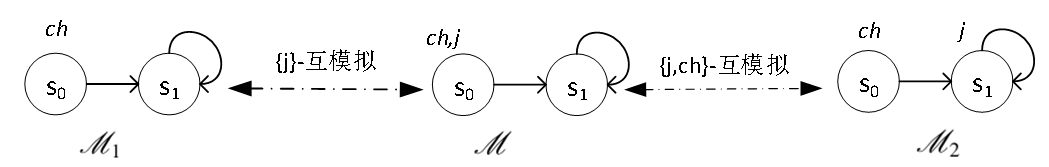
\includegraphics[scale=0.4]{figures/partial_order2}
%%			\caption{初始结构间的$\leq_{\Hm}$关系。}\label{fig:partialo} 
%%		\end{figure}
%	\end{example}}
%	\only<2>{
%		\begin{theorem}\label{thm:minU}
%			给定$\mu$-句子$\Gamma$和$\varphi$,则:
%			\[\Mod(\Gamma \diamond_{\CTL} \varphi) = \bigcup_{\Hm\in \Mod(\Gamma)} Min(\Mod(\varphi), \leq_{\Hm}).
%			\]
%			其中,$Min(\Mod(\varphi), \leq_{\Hm})$是$\varphi$的关于偏序关系$\leq_{\Hm}$的极小模型集。
%		\end{theorem}
%		
%		\begin{theorem}\label{thm:U1toU8}
%			知识更新操作$\diamond_{\CTL}$满足Katsuno和Mendelzon提出的基本条件(U1)-(U8)。
%		\end{theorem}
%%		\begin{definition}
%%			给定公式$\Gamma$和$\varphi$。知识更新操作$\diamond_{\CTL}$定义如下:
%%			$$\Mod(\Gamma \diamond \varphi) = \bigcup_{I \in \Mod(\Gamma)} Min(\Mod(\varphi), \leq_{\Hm}).$$
%%		\end{definition}
%	}
%\textcolor{red}{从而为系统正确性和系统更新提供了理论依据。}
%	}
%\end{frame}

%\begin{frame}
%	\frametitle{~知识更新——{\footnotesize 相关性质}}
%	{\footnotesize
%		\begin{theorem}\label{thm:minU}
%			给定$\mu$-句子$\Gamma$和$\varphi$,则:
%			\[\Mod(\Gamma \diamond_{\CTL} \varphi) = \bigcup_{\Hm\in \Mod(\Gamma)} Min(\Mod(\varphi), \leq_{\Hm}).
%			\]
%		\end{theorem}
%	
%	\begin{theorem}\label{thm:U1toU8}
%		知识更新操作$\diamond_{\CTL}$满足Katsuno和Mendelzon提出的基本条件(U1)-(U8)。
%	\end{theorem}
%	}
%\end{frame}
	
%\begin{frame}
%	\frametitle{~研究内容(二)知识更新——{\footnotesize 例子}}
%	{\tiny
%		\begin{example}
%			令$\Ha=\{ch, j\}$、$\varphi = \nu X. j \wedge ch \wedge \EXIST \NEXT \EXIST \NEXT X$、 $\psi= \nu X. \neg j \wedge ch \wedge \EXIST \NEXT \EXIST \NEXT X$且Kripke结构的状态空间为 $\{s_0,s_1\}$,则用$\psi$更新$\varphi$计算如下:
%			\begin{columns}
%				\column{0.5\textwidth}
%				\begin{align*}
%					\Mod(\varphi) = & \{((1), r=s_0, L(s_0)=\{ch,j\}, L(s_1)=\{ch,j\}), \\
%					& ((2),  r=s_1, L(s_1)=\{ch,j\}, L(s_0)=\{ch,j\}),\\
%					& ((3),  r=s_0, L(s_0)=\{ch,j\}, L(s_1)={\cal C}), \\
%					& ((4),  r=s_1, L(s_1)=\{ch,j\}, L(s_0)={\cal C}), \\
%					& ((5),  r=s_0, L(s_0)=\{ch,j\}, L(s_1)={\cal C}), \\
%					& ((6),  r=s_1, L(s_1)=\{ch,j\}, L(s_0)={\cal C}), \dots\}\\
%					\Mod(\psi) = & \{((1), r=s_0, L(s_0)=\{ch\}, L(s_1)=\{ch\}),\\
%					& ((2), r=s_1, L(s_1)=\{ch\}, L(s_0)=\{ch\}),\\
%					& ((3), r=s_0, L(s_0)=\{ch\}, L(s_1)={\cal C}),\\
%					& ((4), r=s_1, L(s_1)=\{ch\}, L(s_0)={\cal C}), \\
%					& ((5), r=s_0, L(s_0)=\{ch\}, L(s_1)={\cal C}),\\
%					& ((6), r=s_1, L(s_1)=\{ch\}, L(s_0)={\cal C}), \dots\}
%				\end{align*}
%				其中,四元组$((i), r= s_k, L(s_0)=V_1, L(s_1)=V_1)$表示Kripke结构$(S,r,R,L)$,其中$S=\{s_0, s_1\}$、$r=s_k$ ($r\in \{0,1\}$)、转换关系如图~\ref{fig:knoup}中的(i) ($i \in \{1,2,3,4,5,6\}$)、$s_0$ 和$s_1$分别被 $V_1 \subseteq \{ch,j\}$ 和 $V_2\subseteq \{ch,j\}$标记且${\cal C} \in \{\emptyset, \{j\}, \{ch\}, \{j,ch\}\}$。
%				\column{0.5\textwidth}
%				\begin{figure}
%					\centering
%					%	\tiny
%					\begin{tikzpicture}[scale=0.8]
%						\tikzstyle{every node}=[font=\small,scale=0.8]
%						\node[blueCircle] (s0) at(0,3) {$s_0$};
%						\node[blueCircle] (s1) at(1,3) {$s_1$};
%						\node at(0.5,2.5) {(1)};
%						\draw[->] (s0) -- (s1);
%						\path (s1) edge [loop above]  (s1);
%						\node[blueCircle] (s2) at(2,3) {$s_1$};
%						\node[blueCircle] (s3) at(3,3) {$s_0$};
%						\node at(2.5,2.5) {(2)};
%						\draw[->] (s2) -- (s3);
%						\path (s3) edge [loop above]  (s3);
%						
%						\node[blueCircle] (t0) at(0,1) {$s_0$};
%						\node[blueCircle] (t1) at(1,1) {$s_1$};
%						\node at(0.5,0.5) {(3)};
%						\draw[->] (t0) -- (t1);
%					%	\path (s1) edge   (s0);
%						\path (t1) edge[->,bend right=45] (t0);
%						\node[blueCircle] (t2) at(2,1) {$s_1$};
%						\node[blueCircle] (t3) at(3,1) {$s_0$};
%						\node at(2.5,0.5) {(4)};
%						\draw[->] (t2) -- (t3);
%					%	\path (t3) edge   (t2);
%						\path (t3) edge[->,bend right=45] (t2);
%						
%						\node[blueCircle] (r0) at(0,-1) {$s_0$};
%						\node[blueCircle] (r1) at(1,-1) {$s_1$};
%						\node at(0.5,-1.5) {(5)};
%						\draw[->] (r0) -- (r1);
%						\path (r1) edge [loop above]  (r1);
%						\path (r0) edge [loop above]  (r0);
%						\node[blueCircle] (r2) at(2,-1) {$s_1$};
%						\node[blueCircle] (r3) at(3,-1) {$s_0$};
%						\node at(2.5,-1.5) {(6)};
%						\draw[->] (r2) -- (r3);
%						\path (r2) edge [loop above]  (r2);
%						\path (r3) edge [loop above]  (r3);
%%						
%%						\path (s1) edge[->,bend right=45] (s0);
%%						\path (s0) edge[->,bend left=-45] (s1);
%%						\path (s1) edge[->,bend right=-45] (s2);
%%						\path (s2) edge[->,bend right=-45] (s0); 
%%						\node at(0,-0.5) {{\tiny $I/O$请求}};
%%						\node at(-1,0.5) {{\tiny $I/O$完成}};
%%						\node at(0.7,0.7) {{\tiny 时间片完}};
%%						\node at(-0.2,0.7) {{\tiny 进程调度}};
%						%	\node at(0,-1.5) {${\cal K}_2$}; 
%					\end{tikzpicture}
%					\caption{{\tiny 状态空间为$\{s_0,s_1\}$的六个Kripke结构示意图}\footnote{{\tiny 这里只列出部分转换关系,其余转换关系可以容易地枚举出来。}}}\label{fig:knoup} 
%				\end{figure}
%%					\begin{figure} 
%%				%	\renewcommand{\figurename}{\zihao{10}图}
%%					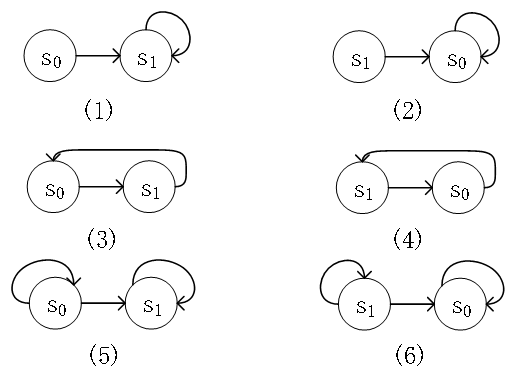
\includegraphics[scale=0.4]{figures/knowledge_update}
%%					\caption{{\tiny 状态空间为$\{s_0,s_1\}$的六个Kripke结构示意图}\footnote{这里只列出部分转换关系,其余转换关系可以容易地枚举出来。}}\label{fig:knoup} 
%%				\end{figure}
%			\end{columns}
%			 
%			$\Mod(\varphi \diamond_{\mu} \psi) = \bigcup_{\Hm\in \Mod(\varphi)} Min(\Mod(\psi), \leq_{\Hm})$,根据定义~\ref{def:closer}容易检查$\Mod(\varphi \diamond_{\mu} \psi) = \Mod(\psi)$。直观地说,由于在$\psi$中$j$在偶数状态不再为真、$ch$保持为真且$\psi$和$\varphi$都不知道模型偶数状态的信息,因而用$\psi$更新$\varphi$得到的结果为 $\psi$自身。 
%		\end{example}
%	}
%\end{frame}

\section{研究内容(三)CTL遗忘计算方法}
\subsection{研究内容(三)简介}
\begin{frame}
	\frametitle{研究内容(三)简介}
	\begin{itemize}
		\item 基于模型的计算方法;
		\item 基于归结的计算方法(CTL-forget算法);
		\item 基于Prolog的CTL-forget算法实现。
	\end{itemize}
\begin{figure}
	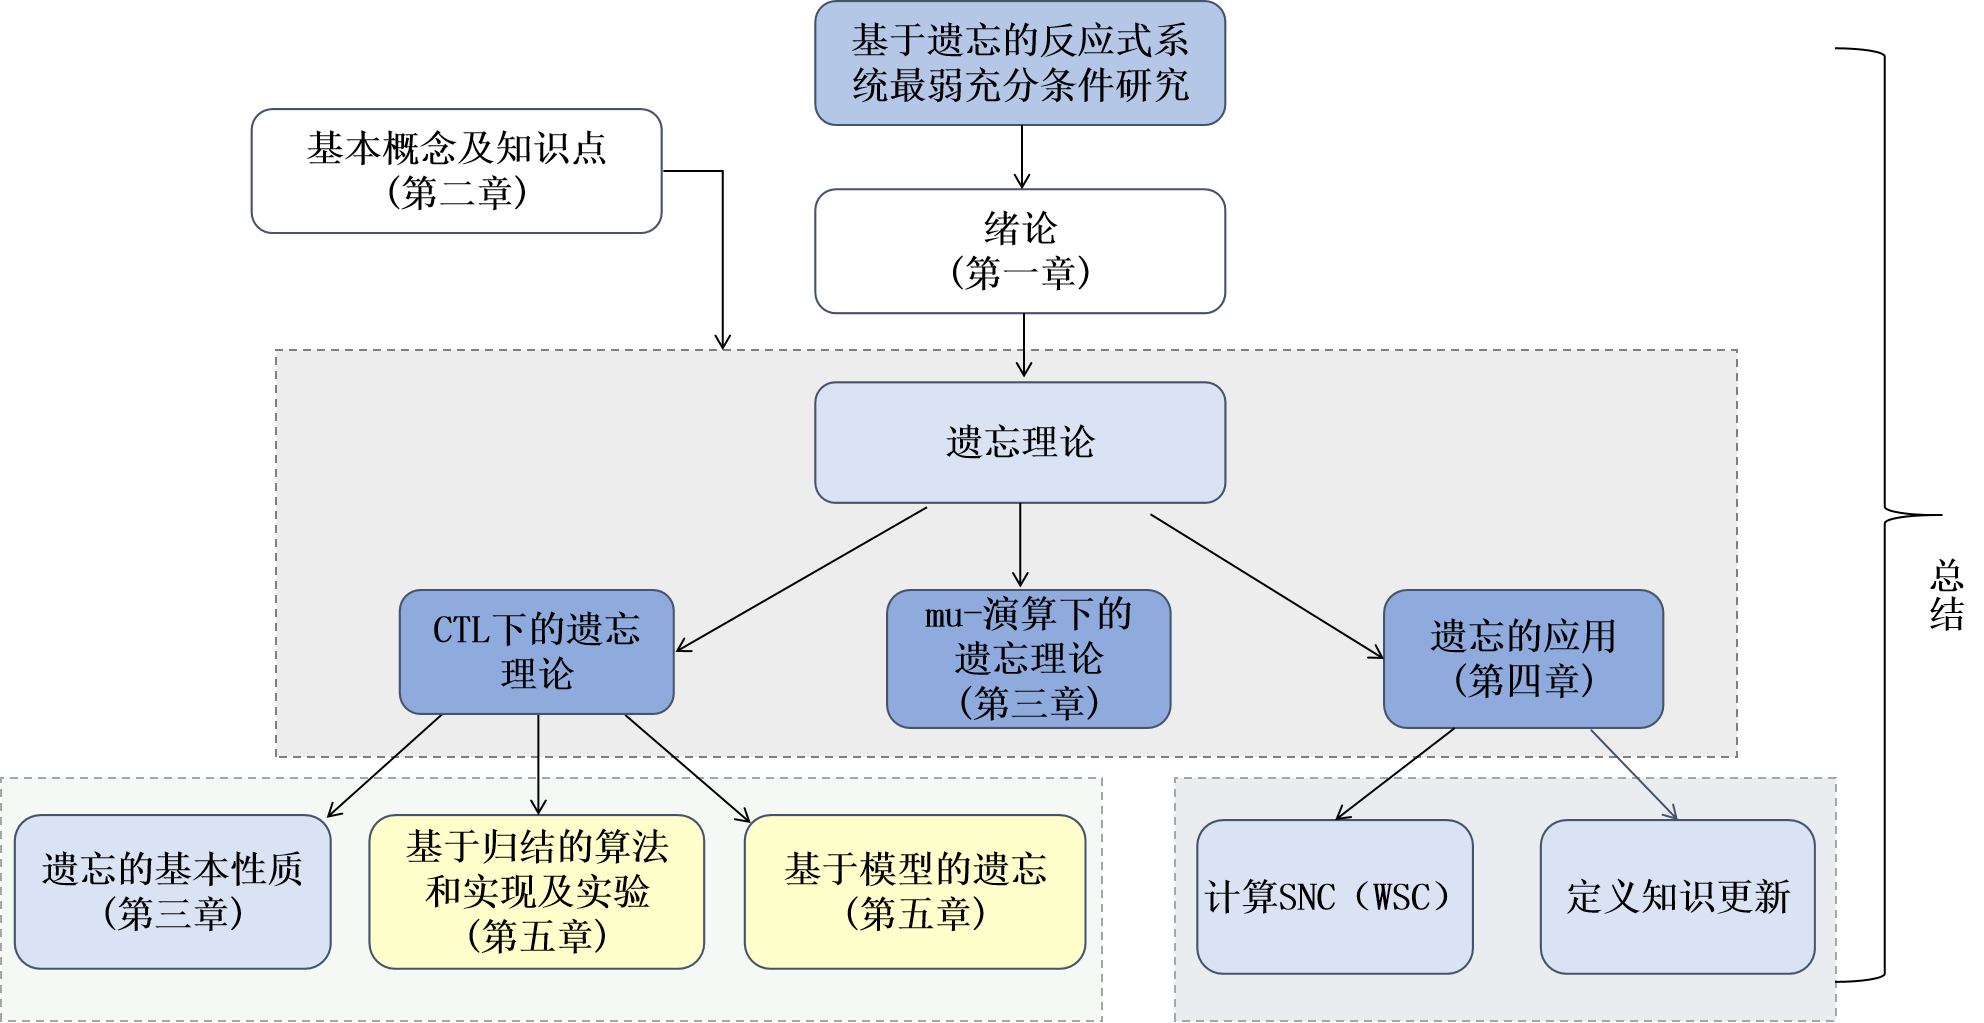
\includegraphics[scale=0.3]{figures/frameF5}
\end{figure}
\end{frame}

\subsection{研究内容(三)(1)基于模型的计算方法}
\begin{frame}
	\frametitle{研究内容(三)(1)基于模型的计算方法}
	%	\begin{figure}
	%		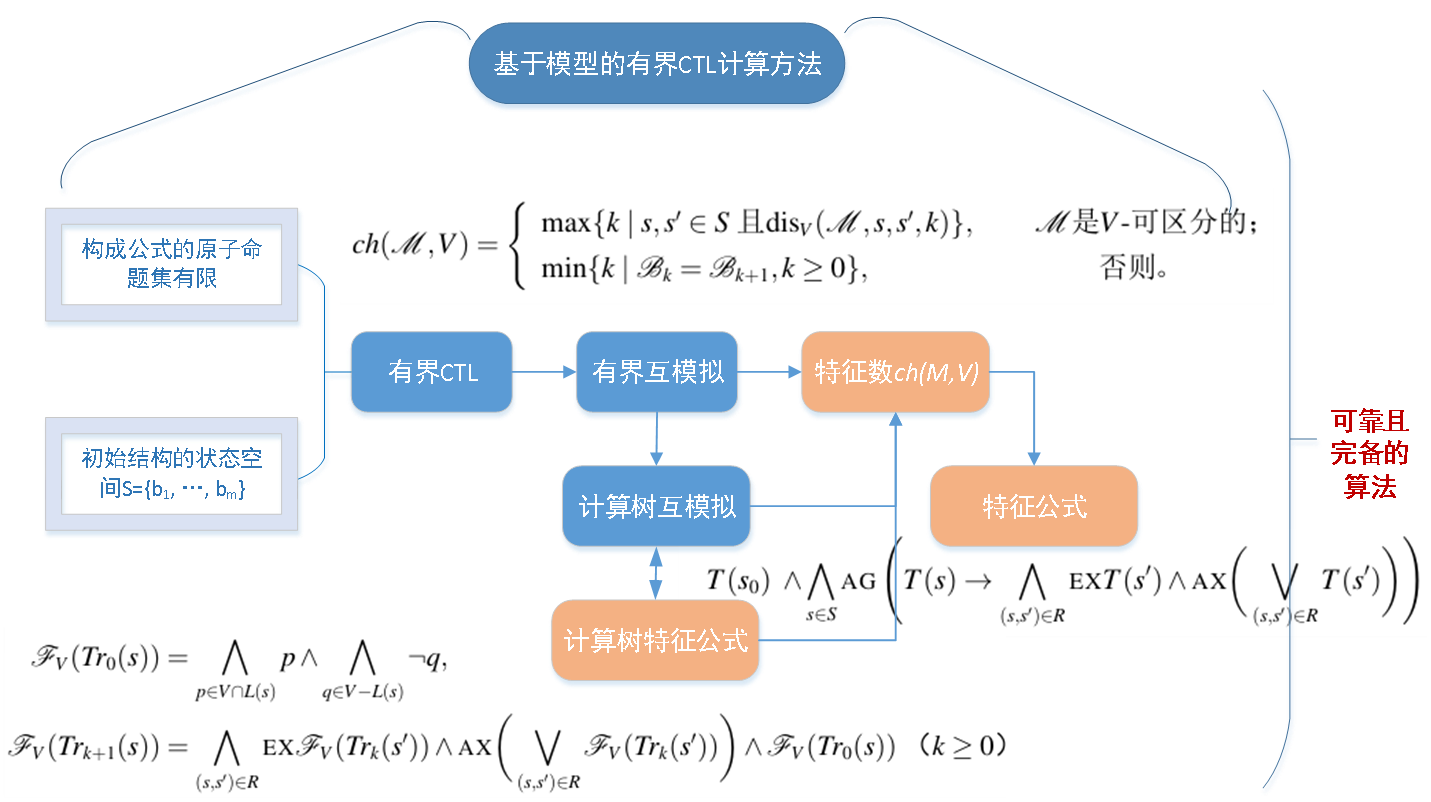
\includegraphics[scale=0.45]{figures/model-basedFrame}
	%		\caption{基于模型的有界CTL遗忘方法}
	%	\end{figure}
	\begin{figure}
		\centering
		%	\tiny
		\begin{tikzpicture}[scale=0.8]
			\tikzstyle{every node}=[font=\small,scale=0.8]
			\node[rectangle,rounded corners =10pt,minimum width =50pt, minimum height =20pt,draw=blue,fill=blue!40] (s0) at(-1,6) {基于模型的有界$\CTL$计算方法};
			\node[color=orange] at(-1, 5.2) {遗忘总是$\CTL$可表示的};
			
			
			
			\node[rectangle,rounded corners =4pt,minimum width =40pt, minimum height =15pt,draw=blue,fill=blue!20] (s1) at(-2,3) {{\scriptsize 有界$\CTL$}};
			
			\node[rectangle, minimum width =50pt, minimum height =15pt,draw=blue,fill=blue!10] (t1) at(-5,3.5) {{\scriptsize 构成公式的原子命题集有限}};
			
			\node[rectangle, minimum width =50pt, minimum height =15pt,draw=blue,fill=blue!10] (t2) at(-5.5,2.5) {{\scriptsize 初始结构的状态空间${\cal S}=\{b_1,\dots, b_m\}$}};
			%	\draw[brace] (-3,3.5) -- (-3,2.5);
			%\node at(-3,3.5) {$}$};
			%	\node at(-2,3) {$\begin{array}{ll}\\ \end{array}$};
			
			\draw[->] (-2.7,3) -- (-3.6,3.5);
			\draw[->] (-2.7,3) -- (-3.6,2.5);
			
			
			\node[rectangle,rounded corners =4pt,minimum width =40pt, minimum height =15pt,draw=blue,fill=blue!20] (s2) at(0,3) {{\scriptsize 有界互模拟}};
			\node[rectangle,rounded corners =4pt,minimum width =40pt, minimum height =15pt,draw=orange,fill=orange!20] (s3) at(2,3) {{\scriptsize 特征数$ch(\Hm,V)$}};
			\node[rectangle,rounded corners =4pt,minimum width =40pt, minimum height =15pt,draw=blue,fill=blue!20] (s4) at(0,2) {{\scriptsize 计算树互模拟}};
			
			\node[rectangle,rounded corners =4pt,minimum width =40pt, minimum height =15pt,draw=orange,fill=orange!20] (s5) at(0,0) {{\scriptsize 计算树特征公式}};
			
			\node[rectangle,rounded corners =4pt,minimum width =40pt, minimum height =15pt,draw=green,fill=green!20] (s6) at(3,2) {{\scriptsize 特征公式}};
			
			
			
			%			\node[rectangle,rounded corners =4pt,minimum width =40pt, minimum height =15pt,draw=red,fill=red!20] (alg2) at(-6,1)[draw,align=center] {{\scriptsize $O((n-x)m^{2(m+2)}2^{nm}  \log m)$} \\ {\scriptsize($m=|{\cal S}|$, $n=|\Ha|$, $x=|V|$)}};
			
			
			%			\\ 
			%		{\scriptsize $\CTLforget(\varphi, V) \models^? \CTLforget(\psi, V)~(\Pi_2^{\textsc{P}}-C)$}; 
			
			%	\draw[->] (alg1) -- (alg2);
			
			%			令 $\varphi$为$\CTL$公式,$V\subseteq \Ha$为原子命题集,状态空间大小为 $|{\cal S}|=m$, $|\Ha|=n$,$|V|=x$。使用算法5.1计算从$\varphi$中遗忘$V$中原子的空间复杂度为 $O((n-x)m^{2(m+2)}2^{nm}  \log m)$,且时间复杂性至少与空间复杂性相同。
			
			
			
			
			
			
			\draw[->] (s1) -- (s2);
			\draw[->] (s2) -- (s3);
			\draw[->] (s2) -- (s4);
			\draw[<->,dashed,color=gray] (s4) -- (s5);
			\draw[->] (s4) -- (2,2)--(s3);
			\draw[->,dashed,color=gray] (s5) -- (2,0) -- (s3);
			\draw[->] (s3) -- (3,3) -- (s6);
			%			\node[blueCircle] (s0) at(0,1) {{\tiny 就绪}};
			%			\node[blueCircle1] (s1) at(0.8,-0.2) {{\tiny 执行}};
			%			\node[redCircle] (s2) at(-0.8,-0.2) {{\tiny 阻塞}};  
			%			\path (s1) edge[->,bend right=45] (s0);
			%			\path (s0) edge[->,bend left=-45] (s1);
			%			\path (s1) edge[->,bend right=-45] (s2);
			%			\path (s2) edge[->,bend right=-45] (s0); 
			%			\node at(0,-0.5) {{\tiny $I/O$请求}};
			%			\node at(-1,0.5) {{\tiny $I/O$完成}};
			%			\node at(0.7,0.7) {{\tiny 时间片完}};
			%			\node at(-0.2,0.7) {{\tiny 进程调度}};
			%	\node at(0,-1.5) {${\cal K}_2$}; 
			%框框
			\draw[dashed, color=blue!20] (-3,6) -- (-7.5,5);
			\draw[dashed, color=blue!20] (1,6) -- (5.5,5);
			\draw[dashed, color=blue!20] (-7.5,5) rectangle (5.5,-1);
		\end{tikzpicture}
		\caption{基于模型的有界CTL遗忘方法}
	\end{figure}
\end{frame}

%\subsection{研究内容(三)(1)基于模型的计算方法}
\begin{frame}
	\frametitle{研究内容(三)(1)基于模型的计算方法}
	%	\begin{figure}
	%		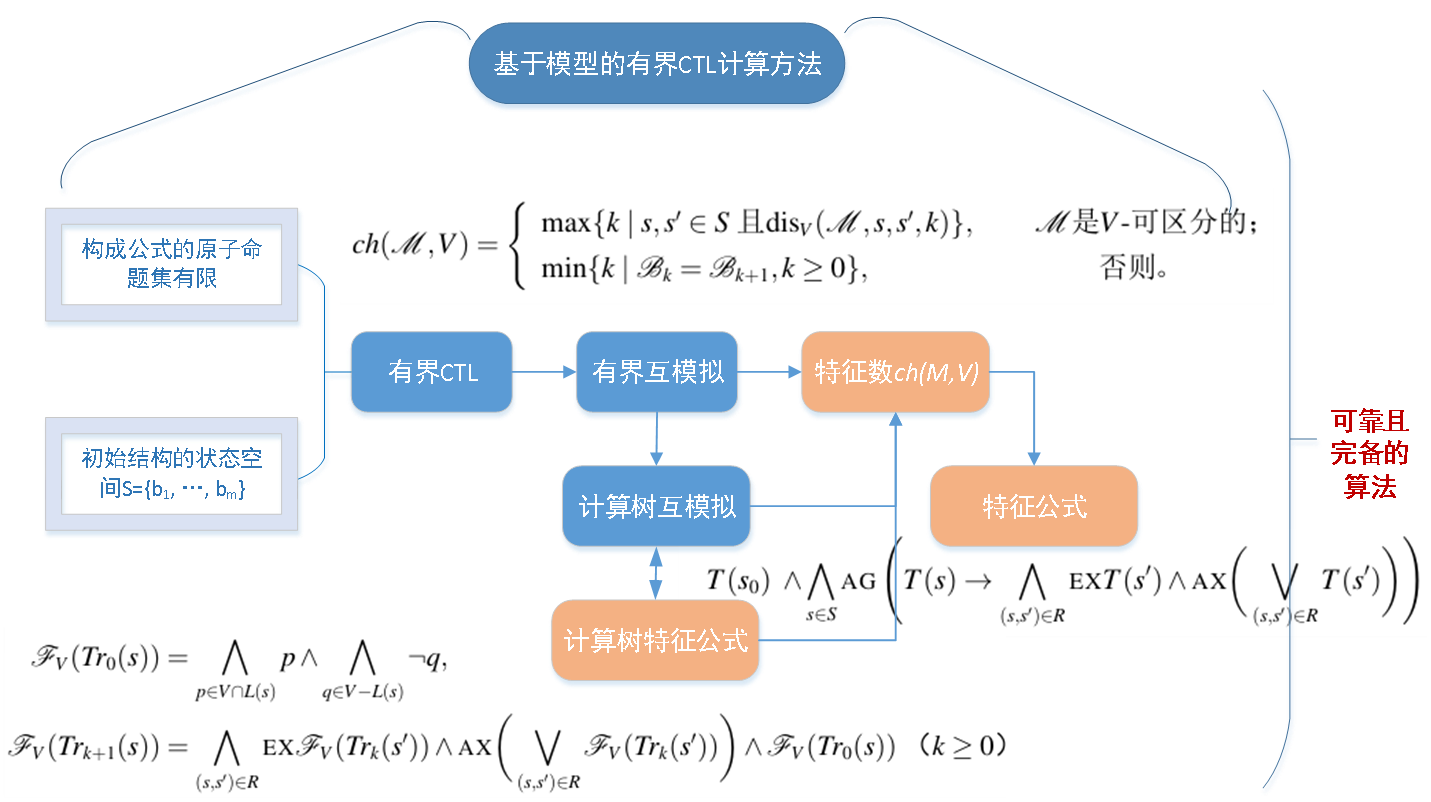
\includegraphics[scale=0.45]{figures/model-basedFrame}
	%		\caption{基于模型的有界CTL遗忘方法}
	%	\end{figure}
	\begin{figure}
		\centering
		%	\tiny
		\begin{tikzpicture}[scale=0.8]
			\tikzstyle{every node}=[font=\small,scale=0.8]
			\node[rectangle,rounded corners =10pt,minimum width =50pt, minimum height =20pt,draw=blue,fill=blue!40] (s0) at(-1,6) {基于模型的有界$\CTL$计算方法};
			\node[color=orange] at(-1, 5.2) {遗忘总是$\CTL$可表示的};
			 
			
			
			\node[rectangle,rounded corners =4pt,minimum width =40pt, minimum height =15pt,draw=blue,fill=blue!20] (s1) at(-2,3) {{\scriptsize 有界$\CTL$}};
			
			\node[rectangle, minimum width =50pt, minimum height =15pt,draw=blue,fill=blue!10] (t1) at(-5,3.5) {{\scriptsize 构成公式的原子命题集有限}};
			
			\node[rectangle, minimum width =50pt, minimum height =15pt,draw=blue,fill=blue!10] (t2) at(-5.5,2.5) {{\scriptsize 初始结构的状态空间${\cal S}=\{b_1,\dots, b_m\}$}};
			%	\draw[brace] (-3,3.5) -- (-3,2.5);
			%\node at(-3,3.5) {$}$};
			%	\node at(-2,3) {$\begin{array}{ll}\\ \end{array}$};
			
			\draw[->] (-2.7,3) -- (-3.6,3.5);
			\draw[->] (-2.7,3) -- (-3.6,2.5);
			
			
			\node[rectangle,rounded corners =4pt,minimum width =40pt, minimum height =15pt,draw=blue,fill=blue!20] (s2) at(0,3) {{\scriptsize 有界互模拟}};
			\node[rectangle,rounded corners =4pt,minimum width =40pt, minimum height =15pt,draw=orange,fill=orange!20] (s3) at(2,3) {{\scriptsize 特征数$ch(\Hm,V)$}};
			\node[rectangle,rounded corners =4pt,minimum width =40pt, minimum height =15pt,draw=blue,fill=blue!20] (s4) at(0,2) {{\scriptsize 计算树互模拟}};
			
			\node[rectangle,rounded corners =4pt,minimum width =40pt, minimum height =15pt,draw=orange,fill=orange!20] (s5) at(0,0) {{\scriptsize 计算树特征公式}};
			
			\node[rectangle,rounded corners =4pt,minimum width =40pt, minimum height =15pt,draw=green,fill=green!20] (s6) at(3,2) {{\scriptsize 特征公式}};
			
			\node[circle,minimum width =30pt, minimum height =30pt, fill=yellow!40] (alg1) at(-3,1) {{\scriptsize 可靠且完备\linebreak 的算法}};
			
			%			\node[rectangle,rounded corners =4pt,minimum width =40pt, minimum height =15pt,draw=red,fill=red!20] (alg2) at(-6,1)[draw,align=center] {{\scriptsize $O((n-x)m^{2(m+2)}2^{nm}  \log m)$} \\ {\scriptsize($m=|{\cal S}|$, $n=|\Ha|$, $x=|V|$)}};
			\node[color=red] at(-5.7,2) {{\scriptsize$\CTL_{\ALL \FUTURE}$}};
			\draw[->,color=red!20,dashed] (-2.65,2.8) -- (-4.2,1.8);
			\node[rectangle,rounded corners =4pt,minimum width =40pt, minimum height =15pt,draw=red,fill=yellow!40] (alg2) at(-5.7,1)[draw,align=center] {{\tiny  $\CTLforget(\varphi, V) \models^? \CTLforget(\psi, V)~(\Pi_2^{\textsc{P}}-C)$}\\ {\tiny $(\Hm,s_0)\models^? \CTLforget(\varphi, V)~(\textsc{NP}-C)$} \\ {\tiny $\CTLforget(\varphi, V ) \models^? \psi~(\textsc{NP}-C)$}\\
				{\tiny $\psi \models^? \CTLforget(\varphi, V)~(\Pi_2^{\textsc{P}}-C)$}};
			%			\\ 
			%		{\scriptsize $\CTLforget(\varphi, V) \models^? \CTLforget(\psi, V)~(\Pi_2^{\textsc{P}}-C)$}; 
			
			%	\draw[->] (alg1) -- (alg2);
			
			%			令 $\varphi$为$\CTL$公式,$V\subseteq \Ha$为原子命题集,状态空间大小为 $|{\cal S}|=m$, $|\Ha|=n$,$|V|=x$。使用算法5.1计算从$\varphi$中遗忘$V$中原子的空间复杂度为 $O((n-x)m^{2(m+2)}2^{nm}  \log m)$,且时间复杂性至少与空间复杂性相同。
			
			\draw[->,line width =5pt,color=red!60] (-1.3,2.2) -- (-2, 1.5);
			
			 
			
		 
			
			\draw[->] (s1) -- (s2);
			\draw[->] (s2) -- (s3);
			\draw[->] (s2) -- (s4);
			\draw[<->,dashed,color=gray] (s4) -- (s5);
			\draw[->] (s4) -- (2,2)--(s3);
			\draw[->,dashed,color=gray] (s5) -- (2,0) -- (s3);
			\draw[->] (s3) -- (3,3) -- (s6);
			%			\node[blueCircle] (s0) at(0,1) {{\tiny 就绪}};
			%			\node[blueCircle1] (s1) at(0.8,-0.2) {{\tiny 执行}};
			%			\node[redCircle] (s2) at(-0.8,-0.2) {{\tiny 阻塞}};  
			%			\path (s1) edge[->,bend right=45] (s0);
			%			\path (s0) edge[->,bend left=-45] (s1);
			%			\path (s1) edge[->,bend right=-45] (s2);
			%			\path (s2) edge[->,bend right=-45] (s0); 
			%			\node at(0,-0.5) {{\tiny $I/O$请求}};
			%			\node at(-1,0.5) {{\tiny $I/O$完成}};
			%			\node at(0.7,0.7) {{\tiny 时间片完}};
			%			\node at(-0.2,0.7) {{\tiny 进程调度}};
			%	\node at(0,-1.5) {${\cal K}_2$}; 
			%框框
			\draw[dashed, color=blue!20] (-3,6) -- (-7.5,5);
			\draw[dashed, color=blue!20] (1,6) -- (5.5,5);
			\draw[dashed, color=blue!20] (-7.5,5) rectangle (5.5,-1);
		\end{tikzpicture}
		\caption{基于模型的有界CTL遗忘方法}
	\end{figure}
\end{frame}






%\subsection{研究内容(三)(1)基于模型的计算方法}
\begin{frame}
	\frametitle{研究内容(三)(1)基于模型的计算方法}
	%	\begin{figure}
	%		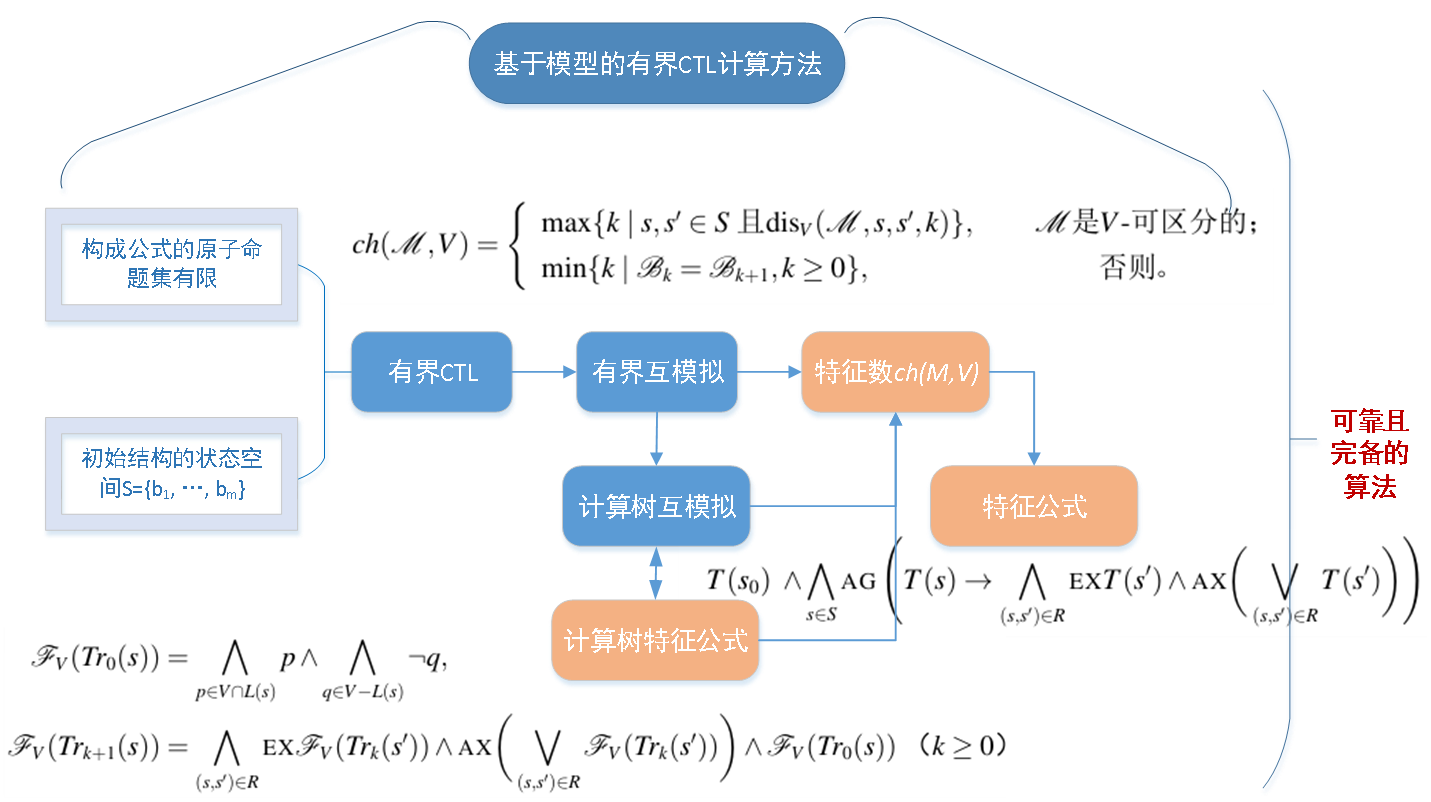
\includegraphics[scale=0.45]{figures/model-basedFrame}
	%		\caption{基于模型的有界CTL遗忘方法}
	%	\end{figure}
	\begin{figure}
		\centering
		%	\tiny
		\begin{tikzpicture}[scale=0.8]
			\tikzstyle{every node}=[font=\small,scale=0.8]
			\node[rectangle,rounded corners =10pt,minimum width =50pt, minimum height =20pt,draw=blue,fill=blue!40] (s0) at(-1,6) {基于模型的有界$\CTL$计算方法};
			\node[color=orange] at(-1, 5.2) {遗忘总是$\CTL$可表示的};
			\node[color=red] at(0,4) {{\scriptsize $
					ch({\cal M},V)=
					\left\{
					\begin{array}{ll}
						\max\{k\mid s,s'\in S \text{ 且 }\dis_V({\cal M},s,s',k)\}, \qquad \hbox{${\cal M}$是 $V$-可区分的;} \\
						\min\{k\mid {\cal B}_{k}={\cal B}_{k+1}, k\ge 0\}, \ \ \ \quad  \qquad \qquad \qquad \hbox{否则。}
					\end{array}
					\right.$}};
			\draw[dashed, color=yellow,fill=yellow!40,opacity=0.2] (-3.8,4.5) rectangle (3.5,3.5);
			
			
			\node[rectangle,rounded corners =4pt,minimum width =40pt, minimum height =15pt,draw=blue,fill=blue!20] (s1) at(-2,3) {{\scriptsize 有界$\CTL$}};
			
			\node[rectangle, minimum width =50pt, minimum height =15pt,draw=blue,fill=blue!10] (t1) at(-5,3.5) {{\scriptsize 构成公式的原子命题集有限}};
			
			\node[rectangle, minimum width =50pt, minimum height =15pt,draw=blue,fill=blue!10] (t2) at(-5.5,2.5) {{\scriptsize 初始结构的状态空间${\cal S}=\{b_1,\dots, b_m\}$}};
			%	\draw[brace] (-3,3.5) -- (-3,2.5);
			%\node at(-3,3.5) {$}$};
			%	\node at(-2,3) {$\begin{array}{ll}\\ \end{array}$};
			
			\draw[->] (-2.7,3) -- (-3.6,3.5);
			\draw[->] (-2.7,3) -- (-3.6,2.5);
			
			
			\node[rectangle,rounded corners =4pt,minimum width =40pt, minimum height =15pt,draw=blue,fill=blue!20] (s2) at(0,3) {{\scriptsize 有界互模拟}};
			\node[rectangle,rounded corners =4pt,minimum width =40pt, minimum height =15pt,draw=orange,fill=yellow!40] (s3) at(2,3) {{\scriptsize 特征数$ch(\Hm,V)$}};
			\node[rectangle,rounded corners =4pt,minimum width =40pt, minimum height =15pt,draw=blue,fill=blue!20] (s4) at(0,2) {{\scriptsize 计算树互模拟}};
			
			\node[rectangle,rounded corners =4pt,minimum width =40pt, minimum height =15pt,draw=orange,fill=orange!20] (s5) at(0,0) {{\scriptsize 计算树特征公式}};
			
			\node[rectangle,rounded corners =4pt,minimum width =40pt, minimum height =15pt,draw=green,fill=green!20] (s6) at(3,2) {{\scriptsize 特征公式}};
			
			\node[circle,minimum width =30pt, minimum height =30pt, fill=red!20] (alg1) at(-3,1) {{\scriptsize 可靠且完备\linebreak 的算法}};
			
			%			\node[rectangle,rounded corners =4pt,minimum width =40pt, minimum height =15pt,draw=red,fill=red!20] (alg2) at(-6,1)[draw,align=center] {{\scriptsize $O((n-x)m^{2(m+2)}2^{nm}  \log m)$} \\ {\scriptsize($m=|{\cal S}|$, $n=|\Ha|$, $x=|V|$)}};
			\node[color=red] at(-5.7,2) {{\scriptsize$\CTL_{\ALL \FUTURE}$}};
			\draw[->,color=red!20,dashed] (-2.65,2.8) -- (-4.2,1.8);
			\node[rectangle,rounded corners =4pt,minimum width =40pt, minimum height =15pt,draw=red,fill=red!20] (alg2) at(-5.7,1)[draw,align=center] {{\tiny  $\CTLforget(\varphi, V) \models^? \CTLforget(\psi, V)~(\Pi_2^{\textsc{P}}-C)$}\\ {\tiny $(\Hm,s_0)\models^? \CTLforget(\varphi, V)~(\textsc{NP}-C)$} \\ {\tiny $\CTLforget(\varphi, V ) \models^? \psi~(\textsc{NP}-C)$}\\
				{\tiny $\psi \models^? \CTLforget(\varphi, V)~(\Pi_2^{\textsc{P}}-C)$}};
			%			\\ 
			%		{\scriptsize $\CTLforget(\varphi, V) \models^? \CTLforget(\psi, V)~(\Pi_2^{\textsc{P}}-C)$}; 
			
			%	\draw[->] (alg1) -- (alg2);
			
			%			令 $\varphi$为$\CTL$公式,$V\subseteq \Ha$为原子命题集,状态空间大小为 $|{\cal S}|=m$, $|\Ha|=n$,$|V|=x$。使用算法5.1计算从$\varphi$中遗忘$V$中原子的空间复杂度为 $O((n-x)m^{2(m+2)}2^{nm}  \log m)$,且时间复杂性至少与空间复杂性相同。
			
			\draw[->,line width =5pt,color=red!60] (-1.3,2.2) -- (-2, 1.5);
			
			 
			
		 
			
			\draw[->] (s1) -- (s2);
			\draw[->] (s2) -- (s3);
			\draw[->] (s2) -- (s4);
			\draw[<->,dashed,color=gray] (s4) -- (s5);
			\draw[->] (s4) -- (2,2)--(s3);
			\draw[->,dashed,color=gray] (s5) -- (2,0) -- (s3);
			\draw[->] (s3) -- (3,3) -- (s6);
			%			\node[blueCircle] (s0) at(0,1) {{\tiny 就绪}};
			%			\node[blueCircle1] (s1) at(0.8,-0.2) {{\tiny 执行}};
			%			\node[redCircle] (s2) at(-0.8,-0.2) {{\tiny 阻塞}};  
			%			\path (s1) edge[->,bend right=45] (s0);
			%			\path (s0) edge[->,bend left=-45] (s1);
			%			\path (s1) edge[->,bend right=-45] (s2);
			%			\path (s2) edge[->,bend right=-45] (s0); 
			%			\node at(0,-0.5) {{\tiny $I/O$请求}};
			%			\node at(-1,0.5) {{\tiny $I/O$完成}};
			%			\node at(0.7,0.7) {{\tiny 时间片完}};
			%			\node at(-0.2,0.7) {{\tiny 进程调度}};
			%	\node at(0,-1.5) {${\cal K}_2$}; 
			%框框
			\draw[dashed, color=blue!20] (-3,6) -- (-7.5,5);
			\draw[dashed, color=blue!20] (1,6) -- (5.5,5);
			\draw[dashed, color=blue!20] (-7.5,5) rectangle (5.5,-1);
		\end{tikzpicture}
		\caption{基于模型的有界CTL遗忘方法}
	\end{figure}
\end{frame}

%\subsection{研究内容(三)(1)基于模型的计算方法}
\begin{frame}
	\frametitle{研究内容(三)(1)基于模型的计算方法}
	%	\begin{figure}
	%		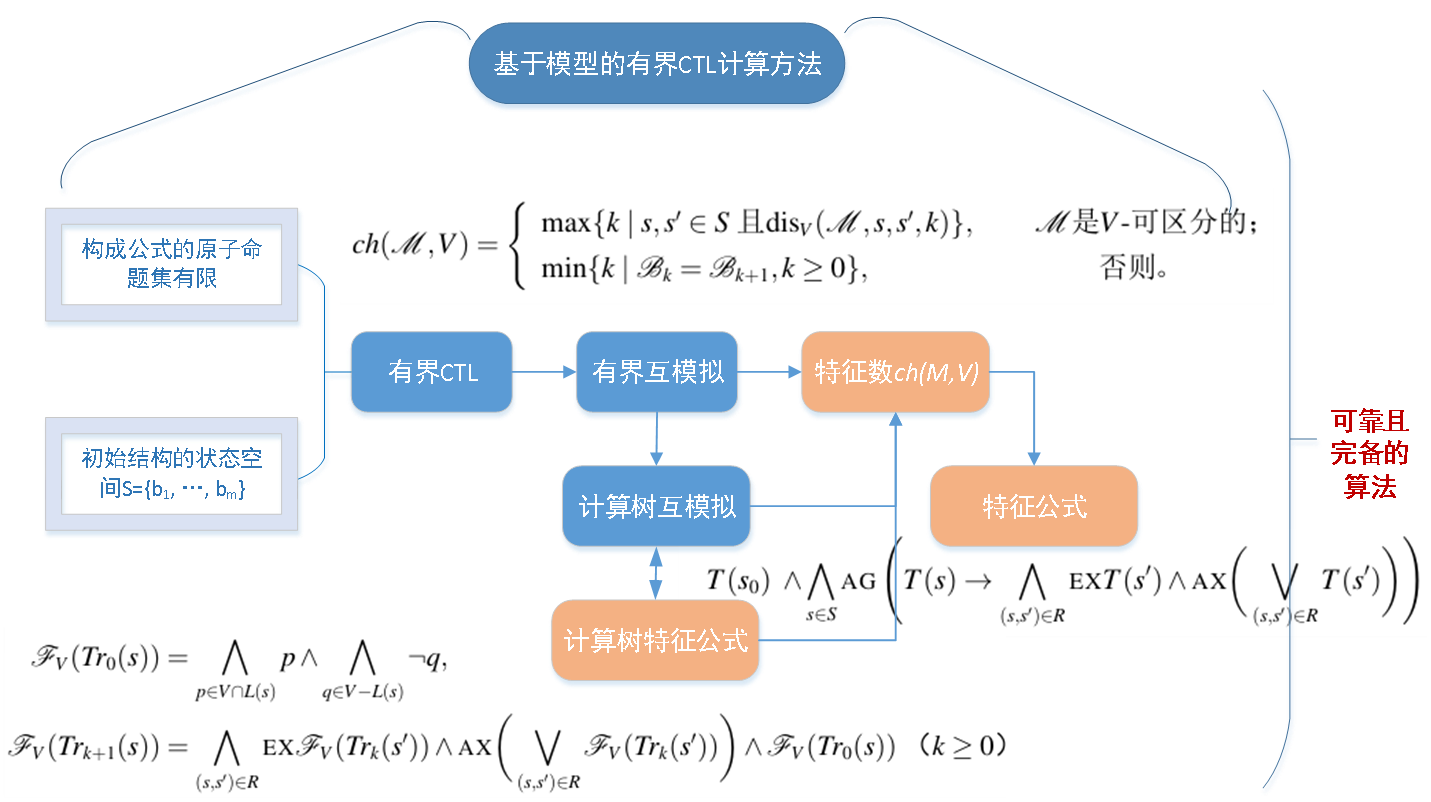
\includegraphics[scale=0.45]{figures/model-basedFrame}
	%		\caption{基于模型的有界CTL遗忘方法}
	%	\end{figure}
	\begin{figure}
		\centering
		%	\tiny
		\begin{tikzpicture}[scale=0.8]
			\tikzstyle{every node}=[font=\small,scale=0.8]
			\node[rectangle,rounded corners =10pt,minimum width =50pt, minimum height =20pt,draw=blue,fill=blue!40] (s0) at(-1,6) {基于模型的有界$\CTL$计算方法};
			\node[color=orange] at(-1, 5.2) {遗忘总是$\CTL$可表示的};
			\node at(0,4) {{\scriptsize $
					ch({\cal M},V)=
					\left\{
					\begin{array}{ll}
						\max\{k\mid s,s'\in S \text{ 且 }\dis_V({\cal M},s,s',k)\}, \qquad \hbox{${\cal M}$是 $V$-可区分的;} \\
						\min\{k\mid {\cal B}_{k}={\cal B}_{k+1}, k\ge 0\}, \ \ \ \quad  \qquad \qquad \qquad \hbox{否则。}
					\end{array}
					\right.$}};
			\draw[dashed, color=orange] (-3.8,4.5) rectangle (3.5,3.5);
			
			
			\node[rectangle,rounded corners =4pt,minimum width =40pt, minimum height =15pt,draw=blue,fill=blue!20] (s1) at(-2,3) {{\scriptsize 有界$\CTL$}};
			
			\node[rectangle, minimum width =50pt, minimum height =15pt,draw=blue,fill=blue!10] (t1) at(-5,3.5) {{\scriptsize 构成公式的原子命题集有限}};
			
			\node[rectangle, minimum width =50pt, minimum height =15pt,draw=blue,fill=blue!10] (t2) at(-5.5,2.5) {{\scriptsize 初始结构的状态空间${\cal S}=\{b_1,\dots, b_m\}$}};
			%	\draw[brace] (-3,3.5) -- (-3,2.5);
			%\node at(-3,3.5) {$}$};
			%	\node at(-2,3) {$\begin{array}{ll}\\ \end{array}$};
			
			\draw[->] (-2.7,3) -- (-3.6,3.5);
			\draw[->] (-2.7,3) -- (-3.6,2.5);
			
			
			\node[rectangle,rounded corners =4pt,minimum width =40pt, minimum height =15pt,draw=blue,fill=blue!20] (s2) at(0,3) {{\scriptsize 有界互模拟}};
			\node[rectangle,rounded corners =4pt,minimum width =40pt, minimum height =15pt,draw=orange,fill=orange!20] (s3) at(2,3) {{\scriptsize 特征数$ch(\Hm,V)$}};
			\node[rectangle,rounded corners =4pt,minimum width =40pt, minimum height =15pt,draw=blue,fill=blue!20] (s4) at(0,2) {{\scriptsize 计算树互模拟}};
			
			\node[rectangle,rounded corners =4pt,minimum width =40pt, minimum height =15pt,draw=orange,fill=yellow!40] (s5) at(0,0) {{\scriptsize 计算树特征公式}};
			
			\node[rectangle,rounded corners =4pt,minimum width =40pt, minimum height =15pt,draw=green,fill=green!20] (s6) at(3,2) {{\scriptsize 特征公式}};
			
			\node[circle,minimum width =30pt, minimum height =30pt, fill=red!20] (alg1) at(-3,1) {{\scriptsize 可靠且完备\linebreak 的算法}};
			
			%			\node[rectangle,rounded corners =4pt,minimum width =40pt, minimum height =15pt,draw=red,fill=red!20] (alg2) at(-6,1)[draw,align=center] {{\scriptsize $O((n-x)m^{2(m+2)}2^{nm}  \log m)$} \\ {\scriptsize($m=|{\cal S}|$, $n=|\Ha|$, $x=|V|$)}};
			\node[color=red] at(-5.7,2) {{\scriptsize$\CTL_{\ALL \FUTURE}$}};
			\draw[->,color=red!20,dashed] (-2.65,2.8) -- (-4.2,1.8);
			\node[rectangle,rounded corners =4pt,minimum width =40pt, minimum height =15pt,draw=red,fill=red!20] (alg2) at(-5.7,1)[draw,align=center] {{\tiny  $\CTLforget(\varphi, V) \models^? \CTLforget(\psi, V)~(\Pi_2^{\textsc{P}}-C)$}\\ {\tiny $(\Hm,s_0)\models^? \CTLforget(\varphi, V)~(\textsc{NP}-C)$} \\ {\tiny $\CTLforget(\varphi, V ) \models^? \psi~(\textsc{NP}-C)$}\\
				{\tiny $\psi \models^? \CTLforget(\varphi, V)~(\Pi_2^{\textsc{P}}-C)$}};
			%			\\ 
			%		{\scriptsize $\CTLforget(\varphi, V) \models^? \CTLforget(\psi, V)~(\Pi_2^{\textsc{P}}-C)$}; 
			
			%	\draw[->] (alg1) -- (alg2);
			
			%			令 $\varphi$为$\CTL$公式,$V\subseteq \Ha$为原子命题集,状态空间大小为 $|{\cal S}|=m$, $|\Ha|=n$,$|V|=x$。使用算法5.1计算从$\varphi$中遗忘$V$中原子的空间复杂度为 $O((n-x)m^{2(m+2)}2^{nm}  \log m)$,且时间复杂性至少与空间复杂性相同。
			
			\draw[->,line width =5pt,color=red!60] (-1.3,2.2) -- (-2, 1.5);
			
			 
			
			\node[color=red] at(-3.5,-0.2) {{\scriptsize $
					{\cal F}_V(\Tr_0(s)) =  \bigwedge_{p \in V\cap L(s)}p
					\wedge \bigwedge_{q\in V-L(s)} \neg q,$  
			}};
			\node[color=red] at(-1, -0.6) {{\scriptsize${\cal F}_V(\Tr_{k+1}(s)) = \bigwedge_{(s,s')\in R}
					\EXIST \NEXT {\cal F}_V(\Tr_k(s')) 
					\wedge  
					\ALL \NEXT \bigg( \bigvee_{(s,s')\in R} {\cal F}_V(\Tr_k(s')) \bigg) \wedge {\cal F}_V(\Tr_0(s))$ ($k\ge 0$)}}; %计算树特征公式
			\draw[dashed, color=yellow,fill=yellow!40,opacity=0.2] (-5.8,0) rectangle (3.8,-1);
			
			\draw[->] (s1) -- (s2);
			\draw[->] (s2) -- (s3);
			\draw[->] (s2) -- (s4);
			\draw[<->,dashed,color=gray] (s4) -- (s5);
			\draw[->] (s4) -- (2,2)--(s3);
			\draw[->,dashed,color=gray] (s5) -- (2,0) -- (s3);
			\draw[->] (s3) -- (3,3) -- (s6); 
			\draw[dashed, color=blue!20] (-3,6) -- (-7.5,5);
			\draw[dashed, color=blue!20] (1,6) -- (5.5,5);
			\draw[dashed, color=blue!20] (-7.5,5) rectangle (5.5,-1);
		\end{tikzpicture}
		\caption{基于模型的有界CTL遗忘方法}
	\end{figure}
\end{frame}

%\subsection{研究内容(三)(1)基于模型的计算方法}
\begin{frame}
	\frametitle{研究内容(三)(1)基于模型的计算方法}
	%	\begin{figure}
	%		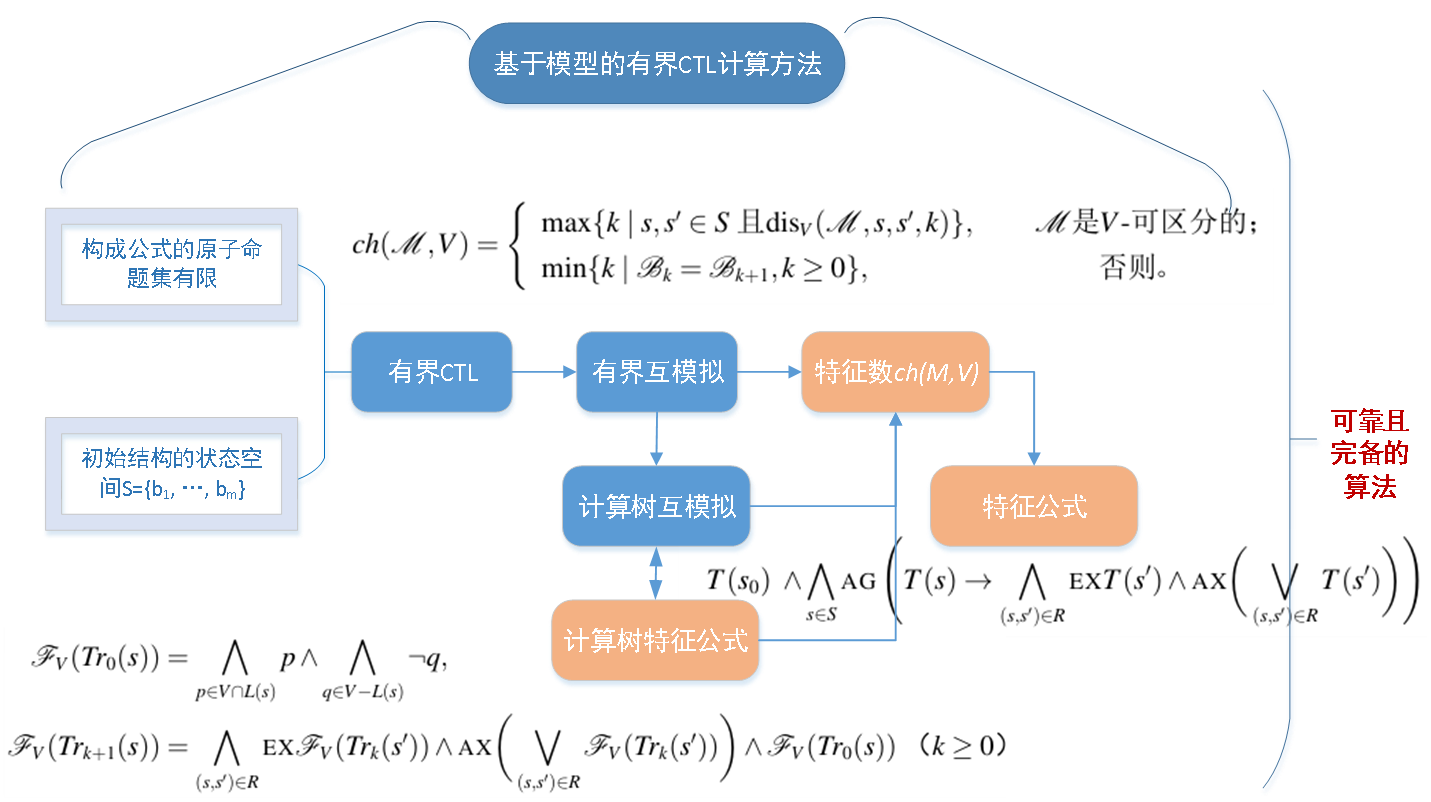
\includegraphics[scale=0.45]{figures/model-basedFrame}
	%		\caption{基于模型的有界CTL遗忘方法}
	%	\end{figure}
	\begin{figure}
		\centering
		%	\tiny
		\begin{tikzpicture}[scale=0.8]
			\tikzstyle{every node}=[font=\small,scale=0.8]
			\node[rectangle,rounded corners =10pt,minimum width =50pt, minimum height =20pt,draw=blue,fill=blue!40] (s0) at(-1,6) {基于模型的有界$\CTL$计算方法};
			\node[color=orange] at(-1, 5.2) {遗忘总是$\CTL$可表示的};
			\node at(0,4) {{\scriptsize $
					ch({\cal M},V)=
					\left\{
					\begin{array}{ll}
						\max\{k\mid s,s'\in S \text{ 且 }\dis_V({\cal M},s,s',k)\}, \qquad \hbox{${\cal M}$是 $V$-可区分的;} \\
						\min\{k\mid {\cal B}_{k}={\cal B}_{k+1}, k\ge 0\}, \ \ \ \quad  \qquad \qquad \qquad \hbox{否则。}
					\end{array}
					\right.$}};
			\draw[dashed, color=orange] (-3.8,4.5) rectangle (3.5,3.5);
			
			
			\node[rectangle,rounded corners =4pt,minimum width =40pt, minimum height =15pt,draw=blue,fill=blue!20] (s1) at(-2,3) {{\scriptsize 有界$\CTL$}};
			
			\node[rectangle, minimum width =50pt, minimum height =15pt,draw=blue,fill=blue!10] (t1) at(-5,3.5) {{\scriptsize 构成公式的原子命题集有限}};
			
			\node[rectangle, minimum width =50pt, minimum height =15pt,draw=blue,fill=blue!10] (t2) at(-5.5,2.5) {{\scriptsize 初始结构的状态空间${\cal S}=\{b_1,\dots, b_m\}$}};
			%	\draw[brace] (-3,3.5) -- (-3,2.5);
			%\node at(-3,3.5) {$}$};
			%	\node at(-2,3) {$\begin{array}{ll}\\ \end{array}$};
			
			\draw[->] (-2.7,3) -- (-3.6,3.5);
			\draw[->] (-2.7,3) -- (-3.6,2.5);
			
			
			\node[rectangle,rounded corners =4pt,minimum width =40pt, minimum height =15pt,draw=blue,fill=blue!20] (s2) at(0,3) {{\scriptsize 有界互模拟}};
			\node[rectangle,rounded corners =4pt,minimum width =40pt, minimum height =15pt,draw=orange,fill=orange!20] (s3) at(2,3) {{\scriptsize 特征数$ch(\Hm,V)$}};
			\node[rectangle,rounded corners =4pt,minimum width =40pt, minimum height =15pt,draw=blue,fill=blue!20] (s4) at(0,2) {{\scriptsize 计算树互模拟}};
			
			\node[rectangle,rounded corners =4pt,minimum width =40pt, minimum height =15pt,draw=orange,fill=orange!20] (s5) at(0,0) {{\scriptsize 计算树特征公式}};
			
			\node[rectangle,rounded corners =4pt,minimum width =40pt, minimum height =15pt,draw=green,fill=yellow!40] (s6) at(3,2) {{\scriptsize 特征公式}};
			
			\node[circle,minimum width =30pt, minimum height =30pt, fill=red!20] (alg1) at(-3,1) {{\scriptsize 可靠且完备\linebreak 的算法}};
			
			%			\node[rectangle,rounded corners =4pt,minimum width =40pt, minimum height =15pt,draw=red,fill=red!20] (alg2) at(-6,1)[draw,align=center] {{\scriptsize $O((n-x)m^{2(m+2)}2^{nm}  \log m)$} \\ {\scriptsize($m=|{\cal S}|$, $n=|\Ha|$, $x=|V|$)}};
			\node[color=red] at(-5.7,2) {{\scriptsize$\CTL_{\ALL \FUTURE}$}};
			\draw[->,color=red!20,dashed] (-2.65,2.8) -- (-4.2,1.8);
			\node[rectangle,rounded corners =4pt,minimum width =40pt, minimum height =15pt,draw=red,fill=red!20] (alg2) at(-5.7,1)[draw,align=center] {{\tiny  $\CTLforget(\varphi, V) \models^? \CTLforget(\psi, V)~(\Pi_2^{\textsc{P}}-C)$}\\ {\tiny $(\Hm,s_0)\models^? \CTLforget(\varphi, V)~(\textsc{NP}-C)$} \\ {\tiny $\CTLforget(\varphi, V ) \models^? \psi~(\textsc{NP}-C)$}\\
				{\tiny $\psi \models^? \CTLforget(\varphi, V)~(\Pi_2^{\textsc{P}}-C)$}};
			%			\\ 
			%		{\scriptsize $\CTLforget(\varphi, V) \models^? \CTLforget(\psi, V)~(\Pi_2^{\textsc{P}}-C)$}; 
			
			%	\draw[->] (alg1) -- (alg2);
			
			%			令 $\varphi$为$\CTL$公式,$V\subseteq \Ha$为原子命题集,状态空间大小为 $|{\cal S}|=m$, $|\Ha|=n$,$|V|=x$。使用算法5.1计算从$\varphi$中遗忘$V$中原子的空间复杂度为 $O((n-x)m^{2(m+2)}2^{nm}  \log m)$,且时间复杂性至少与空间复杂性相同。
			
			\draw[->,line width =5pt,color=red!60] (-1.3,2.2) -- (-2, 1.5);
			
			\node[color=red] at(1,0.5) {{\scriptsize$T(s') = {\cal F}_V(\Tr_c(s'))$}};
			\node[color=red] at(2,1) {{\scriptsize$T(s_0) \text{ } \wedge \bigwedge_{s\in S}\ALL \GLOBAL\left(
					T(s) \rto
					\bigwedge_{(s,s')\in R}
					\EXIST \NEXT T(s')
					\wedge
					\ALL \NEXT \bigg(\bigvee_{(s,s')\in R}T(s')\bigg)
					\right).
					$}}; %特征公式
			
			%\draw[dashed, color=green!40] (-1.3,1.5) rectangle (5.2,0.3);
			\draw[dashed, color=yellow,fill=yellow!40,opacity=0.2] (-1.3,1.5) rectangle (5.2,0.3);
			
			\node at(-3.5,-0.2) {{\scriptsize $
					{\cal F}_V(\Tr_0(s)) =  \bigwedge_{p \in V\cap L(s)}p
					\wedge \bigwedge_{q\in V-L(s)} \neg q,$  
			}};
			\node at(-1, -0.6) {{\scriptsize${\cal F}_V(\Tr_{k+1}(s)) = \bigwedge_{(s,s')\in R}
					\EXIST \NEXT {\cal F}_V(\Tr_k(s')) 
					\wedge  
					\ALL \NEXT \bigg( \bigvee_{(s,s')\in R} {\cal F}_V(\Tr_k(s')) \bigg) \wedge {\cal F}_V(\Tr_0(s))$ ($k\ge 0$)}}; %计算树特征公式
			
			\draw[->] (s1) -- (s2);
			\draw[->] (s2) -- (s3);
			\draw[->] (s2) -- (s4);
			\draw[<->,dashed,color=gray] (s4) -- (s5);
			\draw[->] (s4) -- (2,2)--(s3);
			\draw[->,dashed,color=gray] (s5) -- (2,0) -- (s3);
			\draw[->] (s3) -- (3,3) -- (s6);
			%			\node[blueCircle] (s0) at(0,1) {{\tiny 就绪}};
			%			\node[blueCircle1] (s1) at(0.8,-0.2) {{\tiny 执行}};
			%			\node[redCircle] (s2) at(-0.8,-0.2) {{\tiny 阻塞}};  
			%			\path (s1) edge[->,bend right=45] (s0);
			%			\path (s0) edge[->,bend left=-45] (s1);
			%			\path (s1) edge[->,bend right=-45] (s2);
			%			\path (s2) edge[->,bend right=-45] (s0); 
			%			\node at(0,-0.5) {{\tiny $I/O$请求}};
			%			\node at(-1,0.5) {{\tiny $I/O$完成}};
			%			\node at(0.7,0.7) {{\tiny 时间片完}};
			%			\node at(-0.2,0.7) {{\tiny 进程调度}};
			%	\node at(0,-1.5) {${\cal K}_2$}; 
			%框框
			\draw[dashed, color=blue!20] (-3,6) -- (-7.5,5);
			\draw[dashed, color=blue!20] (1,6) -- (5.5,5);
			\draw[dashed, color=blue!20] (-7.5,5) rectangle (5.5,-1);
		\end{tikzpicture}
		\caption{基于模型的有界CTL遗忘方法}
	\end{figure}
\end{frame}

%%%原图%%%%%%%%
%\subsection{研究内容(三)(1)基于模型的计算方法}
%\begin{frame}
%	\frametitle{研究内容(三)(1)基于模型的计算方法}
%	%	\begin{figure}
%	%		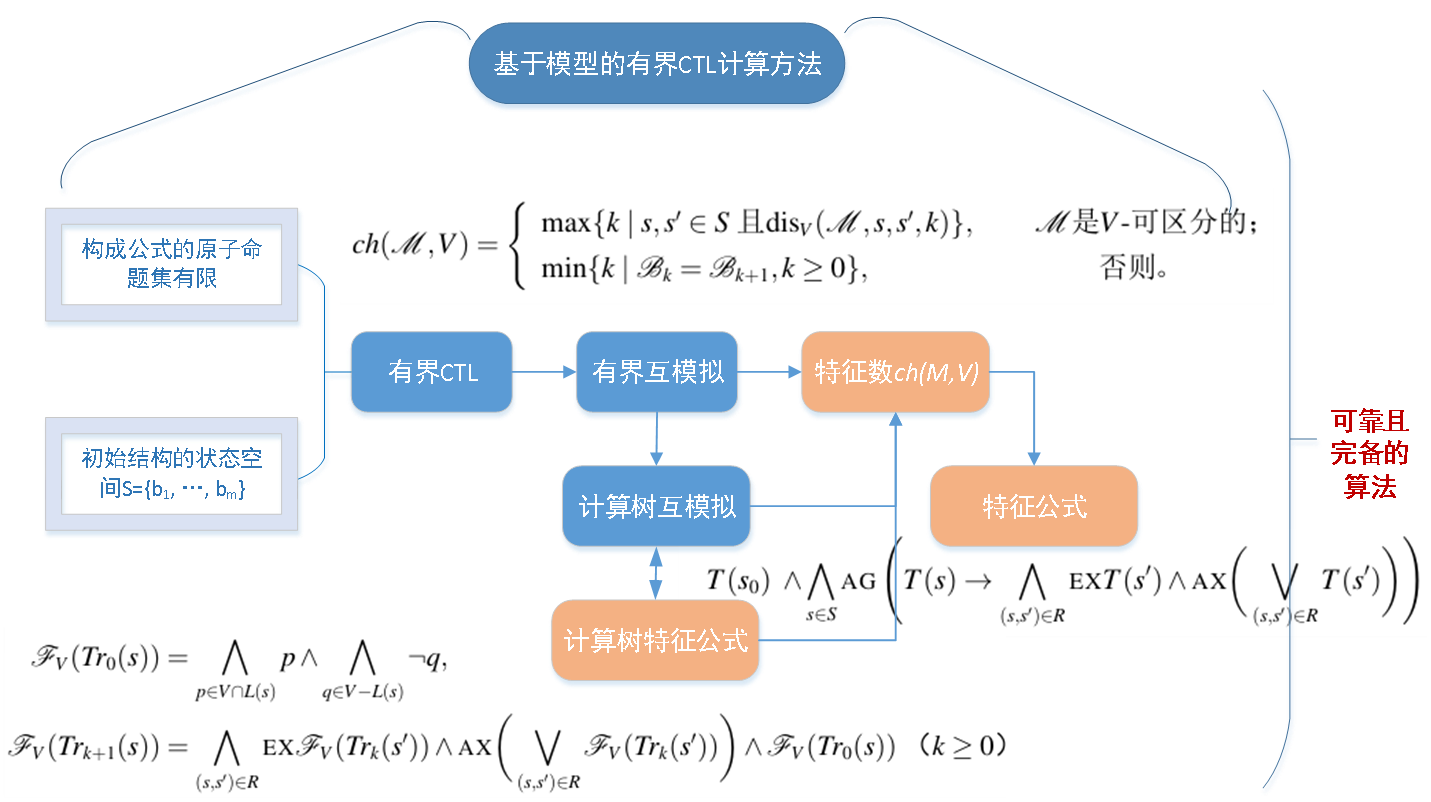
\includegraphics[scale=0.45]{figures/model-basedFrame}
%	%		\caption{基于模型的有界CTL遗忘方法}
%	%	\end{figure}
%	\begin{figure}
%		\centering
%		%	\tiny
%		\begin{tikzpicture}[scale=0.8]
%			\tikzstyle{every node}=[font=\small,scale=0.8]
%			\node[rectangle,rounded corners =10pt,minimum width =50pt, minimum height =20pt,draw=blue,fill=blue!40] (s0) at(-1,6) {基于模型的有界$\CTL$计算方法};
%			\node[color=orange] at(-1, 5.2) {遗忘总是$\CTL$可表示的};
%			\node at(0,4) {{\scriptsize $
%					ch({\cal M},V)=
%					\left\{
%					\begin{array}{ll}
%						\max\{k\mid s,s'\in S \text{ 且 }\dis_V({\cal M},s,s',k)\}, \qquad \hbox{${\cal M}$是 $V$-可区分的;} \\
%						\min\{k\mid {\cal B}_{k}={\cal B}_{k+1}, k\ge 0\}, \ \ \ \quad  \qquad \qquad \qquad \hbox{否则。}
%					\end{array}
%					\right.$}};
%			\draw[dashed, color=orange] (-3.8,4.5) rectangle (3.5,3.5);
%			
%			
%			\node[rectangle,rounded corners =4pt,minimum width =40pt, minimum height =15pt,draw=blue,fill=blue!20] (s1) at(-2,3) {{\scriptsize 有界$\CTL$}};
%			
%			\node[rectangle, minimum width =50pt, minimum height =15pt,draw=blue,fill=blue!10] (t1) at(-5,3.5) {{\scriptsize 构成公式的原子命题集有限}};
%			
%			\node[rectangle, minimum width =50pt, minimum height =15pt,draw=blue,fill=blue!10] (t2) at(-5.5,2.5) {{\scriptsize 初始结构的状态空间${\cal S}=\{b_1,\dots, b_m\}$}};
%			%	\draw[brace] (-3,3.5) -- (-3,2.5);
%			%\node at(-3,3.5) {$}$};
%			%	\node at(-2,3) {$\begin{array}{ll}\\ \end{array}$};
%			
%			\draw[->] (-2.7,3) -- (-3.6,3.5);
%			\draw[->] (-2.7,3) -- (-3.6,2.5);
%			
%			
%			\node[rectangle,rounded corners =4pt,minimum width =40pt, minimum height =15pt,draw=blue,fill=blue!20] (s2) at(0,3) {{\scriptsize 有界互模拟}};
%			\node[rectangle,rounded corners =4pt,minimum width =40pt, minimum height =15pt,draw=orange,fill=orange!20] (s3) at(2,3) {{\scriptsize 特征数$ch(\Hm,V)$}};
%			\node[rectangle,rounded corners =4pt,minimum width =40pt, minimum height =15pt,draw=blue,fill=blue!20] (s4) at(0,2) {{\scriptsize 计算树互模拟}};
%			
%			\node[rectangle,rounded corners =4pt,minimum width =40pt, minimum height =15pt,draw=orange,fill=orange!20] (s5) at(0,0) {{\scriptsize 计算树特征公式}};
%			
%			\node[rectangle,rounded corners =4pt,minimum width =40pt, minimum height =15pt,draw=green,fill=green!20] (s6) at(3,2) {{\scriptsize 特征公式}};
%			
%			\node[circle,minimum width =30pt, minimum height =30pt, fill=red!20] (alg1) at(-3,1) {{\scriptsize 可靠且完备\linebreak 的算法}};
%			
%			%			\node[rectangle,rounded corners =4pt,minimum width =40pt, minimum height =15pt,draw=red,fill=red!20] (alg2) at(-6,1)[draw,align=center] {{\scriptsize $O((n-x)m^{2(m+2)}2^{nm}  \log m)$} \\ {\scriptsize($m=|{\cal S}|$, $n=|\Ha|$, $x=|V|$)}};
%			\node[color=red] at(-5.7,2) {{\scriptsize$\CTL_{\ALL \FUTURE}$}};
%			\draw[->,color=red!20,dashed] (-2.65,2.8) -- (-4.2,1.8);
%			\node[rectangle,rounded corners =4pt,minimum width =40pt, minimum height =15pt,draw=red,fill=red!20] (alg2) at(-5.7,1)[draw,align=center] {{\tiny  $\CTLforget(\varphi, V) \models^? \CTLforget(\psi, V)~(\Pi_2^{\textsc{P}}-C)$}\\ {\tiny $(\Hm,s_0)\models^? \CTLforget(\varphi, V)~(\textsc{NP}-C)$} \\ {\tiny $\CTLforget(\varphi, V ) \models^? \psi~(\textsc{NP}-C)$}\\
%				{\tiny $\psi \models^? \CTLforget(\varphi, V)~(\Pi_2^{\textsc{P}}-C)$}};
%			%			\\ 
%			%		{\scriptsize $\CTLforget(\varphi, V) \models^? \CTLforget(\psi, V)~(\Pi_2^{\textsc{P}}-C)$}; 
%			
%			%	\draw[->] (alg1) -- (alg2);
%			
%			%			令 $\varphi$为$\CTL$公式,$V\subseteq \Ha$为原子命题集,状态空间大小为 $|{\cal S}|=m$, $|\Ha|=n$,$|V|=x$。使用算法5.1计算从$\varphi$中遗忘$V$中原子的空间复杂度为 $O((n-x)m^{2(m+2)}2^{nm}  \log m)$,且时间复杂性至少与空间复杂性相同。
%			
%			\draw[->,line width =5pt,color=red!60] (-1.3,2.2) -- (-2, 1.5);
%			
%			\node[color=blue!90] at(1,0.5) {{\scriptsize$T(s') = {\cal F}_V(\Tr_c(s'))$}};
%			\node[color=blue!90] at(2,1) {{\scriptsize$T(s_0) \text{ } \wedge \bigwedge_{s\in S}\ALL \GLOBAL\left(
%					T(s) \rto
%					\bigwedge_{(s,s')\in R}
%					\EXIST \NEXT T(s')
%					\wedge
%					\ALL \NEXT \bigg(\bigvee_{(s,s')\in R}T(s')\bigg)
%					\right).
%					$}}; %特征公式
%			
%			\draw[dashed, color=green!40] (-1.3,1.5) rectangle (5.2,0.3);
%			
%			\node[color=orange!90] at(-3.5,-0.2) {{\scriptsize $
%					{\cal F}_V(\Tr_0(s)) =  \bigwedge_{p \in V\cap L(s)}p
%					\wedge \bigwedge_{q\in V-L(s)} \neg q,$  
%			}};
%			\node[color=orange!90] at(-1, -0.6) {{\scriptsize${\cal F}_V(\Tr_{k+1}(s)) = \bigwedge_{(s,s')\in R}
%					\EXIST \NEXT {\cal F}_V(\Tr_k(s')) 
%					\wedge  
%					\ALL \NEXT \bigg( \bigvee_{(s,s')\in R} {\cal F}_V(\Tr_k(s')) \bigg) \wedge {\cal F}_V(\Tr_0(s))$ ($k\ge 0$)}}; %计算树特征公式
%			
%			\draw[->] (s1) -- (s2);
%			\draw[->] (s2) -- (s3);
%			\draw[->] (s2) -- (s4);
%			\draw[<->,dashed,color=gray] (s4) -- (s5);
%			\draw[->] (s4) -- (2,2)--(s3);
%			\draw[->,dashed,color=gray] (s5) -- (2,0) -- (s3);
%			\draw[->] (s3) -- (3,3) -- (s6);
%			%			\node[blueCircle] (s0) at(0,1) {{\tiny 就绪}};
%			%			\node[blueCircle1] (s1) at(0.8,-0.2) {{\tiny 执行}};
%			%			\node[redCircle] (s2) at(-0.8,-0.2) {{\tiny 阻塞}};  
%			%			\path (s1) edge[->,bend right=45] (s0);
%			%			\path (s0) edge[->,bend left=-45] (s1);
%			%			\path (s1) edge[->,bend right=-45] (s2);
%			%			\path (s2) edge[->,bend right=-45] (s0); 
%			%			\node at(0,-0.5) {{\tiny $I/O$请求}};
%			%			\node at(-1,0.5) {{\tiny $I/O$完成}};
%			%			\node at(0.7,0.7) {{\tiny 时间片完}};
%			%			\node at(-0.2,0.7) {{\tiny 进程调度}};
%			%	\node at(0,-1.5) {${\cal K}_2$}; 
%			%框框
%			\draw[dashed, color=blue!20] (-3,6) -- (-7.5,5);
%			\draw[dashed, color=blue!20] (1,6) -- (5.5,5);
%			\draw[dashed, color=blue!20] (-7.5,5) rectangle (5.5,-1);
%		\end{tikzpicture}
%		\caption{基于模型的有界CTL遗忘方法}
%	\end{figure}
%\end{frame}




%
%
%\begin{frame}
%	\frametitle{遗忘封闭性}
%	{\footnotesize 
%		\begin{lemma}\label{lem:models:formula}
%				给定$\CTL$公式$\varphi$,下面等式成立:
%				\begin{equation*}
%					\varphi\equiv \bigvee_{(\Hm, s_0)\in\Mod(\varphi)}{\cal F}_{\cal A}(\Hm, s_0).
%				\end{equation*}
%			\end{lemma}
%			\begin{block}{遗忘封闭性}
%				从$\varphi$中遗忘$V$中的元素得到的结果为:
%				\begin{equation*}
%					\bigvee_{{\cal K}\in  \{{\cal K}'\mid \exists {\cal K}''\in\Mod(\phi),\ {\cal K}''\lrto_V{\cal K}'\}} {\cal F}_{\overline V}({\cal K}).
%				\end{equation*}
%		\end{block}
%	}
%\end{frame}

\begin{frame}
	\frametitle{研究内容(三)(1)基于模型的遗忘算法}
	{\footnotesize 
		
		\begin{figure}
			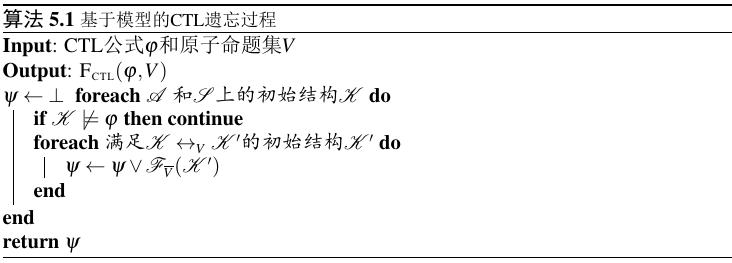
\includegraphics[scale=0.45]{figures/model-basedAlg}
		\end{figure}
		
		\begin{proposition}\label{pro:time:alg1}
			令 $\varphi$为$\CTL$公式,$V\subseteq \Ha$为原子命题集,状态空间大小为 $|{\cal S}|=m$, $|\Ha|=n$,$|V|=x$。使用算法5.1计算从$\varphi$中遗忘$V$中原子的空间复杂度为 $O((n-x)m^{2(m+2)}2^{nm}  \log m)$,且时间复杂性至少与空间复杂性相同。
		\end{proposition}
	}
\end{frame}

 

\subsection{研究内容(三)(2)基于归结的算法CTL-forget}
 

\begin{frame}
	\frametitle{研究内容(三)(2)基于归结的算法CTL-forget}
	{\footnotesize
	
	 
			
		\begin{figure}
			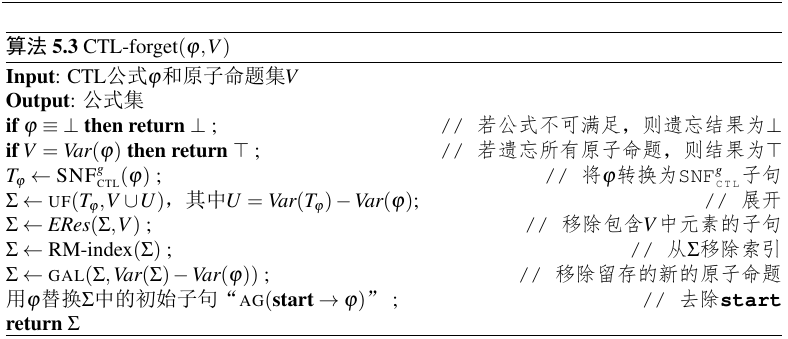
\includegraphics[scale=0.28]{figures/CTL-forget1}
		\end{figure}
%		}
%		\only<2>{	
			\begin{theorem}[可靠性]\label{thm:soundness:forget:algorithm}
				若$\varphi$为一个$\CTL$公式、 $V\subseteq\cal A$、 $\Sigma=$\CTL-forget$(\varphi,V)$且$U=\Var(\Sigma)-\Var(\varphi)$,则:
				\begin{itemize}
					\item[(i)] $\Sigma\equiv_{V\cup U}\varphi$,
					\item[(ii)] 若$U=\emptyset$,则 $\Sigma\equiv\CTLforget(\varphi,V)$。
				\end{itemize}
			\end{theorem}
			
		\begin{proposition} 
			给定$\CTL$公式$\varphi$和原子命题集$V \subseteq \Ha$。
			算法5.3的时间和空间复杂性为{\em $O((m+1)2^{4(n+n')})$},其中$n=|\Var(\varphi)|$、$n'=|V'|$为新引入的原子命题的个数、$m$为引入的索引个数。
		\end{proposition} 
	}
\end{frame}

\begin{frame}
	\frametitle{研究内容(三)(2)基于归结的算法CTL-forget}
	{\footnotesize
		
		
		
		\begin{figure}
			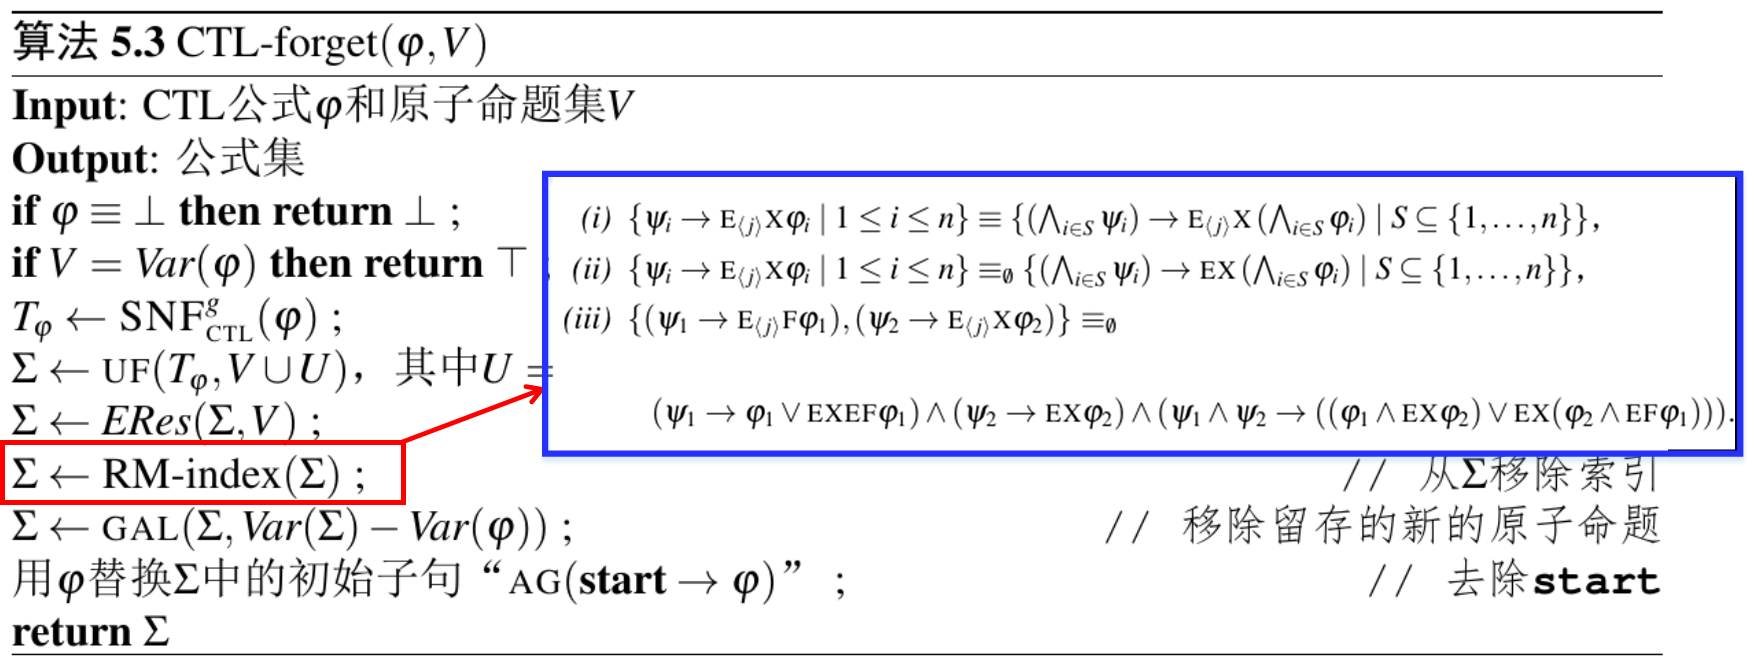
\includegraphics[scale=0.3]{figures/CTL-forget3}
		\end{figure}
		%		}
		%		\only<2>{	
		\begin{theorem}[可靠性] 
			若$\varphi$为一个$\CTL$公式、 $V\subseteq\cal A$、 $\Sigma=$\CTL-forget$(\varphi,V)$且$U=\Var(\Sigma)-\Var(\varphi)$,则:
			\begin{itemize}
				\item[(i)] $\Sigma\equiv_{V\cup U}\varphi$,
				\item[(ii)] 若$U=\emptyset$,则 $\Sigma\equiv\CTLforget(\varphi,V)$。
			\end{itemize}
		\end{theorem}
		
		\begin{proposition} 
			给定$\CTL$公式$\varphi$和原子命题集$V \subseteq \Ha$。
			算法5.3的时间和空间复杂性为{\em $O((m+1)2^{4(n+n')})$},其中$n=|\Var(\varphi)|$、$n'=|V'|$为新引入的原子命题的个数、$m$为引入的索引个数。
		\end{proposition} 
	}
\end{frame}

\subsection{研究内容(三)(3)算法CTL-forget实现及实验} 
%\begin{frame}
%	\frametitle{基于归结的算法CTL-forget实现}
%	{\footnotesize
%		\begin{block}{系统描述}
%			\begin{itemize}
%				\item 输入输出:基于Prolog的$\CTL$-forget算法实现系统以$\CTL$公式和原子命题集为输入,$\CTL$公式为输出;
%				\item 系统识别的$\CTL$公式的符号与第\ref{chapter02}章中$\CTL$的语言符号对应关系如下:
%				\begin{itemize}
%					\item $x_i$和其余小写字母开头的字符串构成原子命题集,其中$i\geq 0$为自然数,且$x_i$和$z$被设定为只能是在如下描述的转换过程中引入的原子命题;%除此之外,约定$z$为保留字(即:在输入的公式中不能包含$z$为命题符号);
%					\item “$false$”和“$true$”分别与常量符号“$\bot$”和“$\top$”对应;
%					\item “$start$”与命题常量“$\start$”对应;
%					\item “$\&$”、“$\backslash/$”、“$-$”和“$->$”分别与联结符号“$\wedge$”、“$\vee$”、“$\neg$”和“$\rto$”对应;%
%					\item “\textasciitilde”和“\textasciicircum”分别与路径量词“$\ALL$”和“$\EXIST$”对应;
%					\item “$@$”、“$*$”、“$?$”和“$\$$”分别与时序操作符“$\GLOBAL$”、“$\NEXT$”、“$\FUTURE$”和“$\UNTILL$”对应。
%				\end{itemize}
%			\end{itemize}
%		\end{block}
%	
%	\begin{example}
%		字符串$($\textasciitilde $* ((-y1\backslash/ -y2\backslash/ -y4)\& (-y1\backslash/y2\backslash/y4)\& (y1\backslash/y2\backslash/ -y3)\& (y1\backslash/y3\backslash/ -y4)\& (-y1\backslash/y2\backslash/ -y3)))$为 $\CTL$ 公式。
%	\end{example}
%	}
%\end{frame}

\begin{frame}
	\frametitle{研究内容(三)(3)算法CTL-forget实现}
	{\footnotesize
		\begin{block}{系统主要模块}
			此系统主要包括五个模块\footnote{ \url{https://github.com/fengrenyan/forgetting-in-CTL/tree/main/Appendix}}:
			\begin{itemize}
				\item 转换模块(transCTL2SNF/6): 
				\item 归结模块(两个过程:step\_resolution/3和temp\_resolution/8)
				\item “移除”原子命题模块(removeAtom/3)
				\item “移除”索引(pro6/3)
				\item “移除”新引入的原子命题(ackerM/3)
			\end{itemize} 
		\end{block}
	}
\end{frame}

\begin{frame}
	\frametitle{研究内容(三)(3)算法CTL-forget实验——{\footnotesize 实验 1:计算遗忘}}
	{\footnotesize
		(1)	标准数据集来源于$\CTL$-RP: \url{https://sourceforge.net/projects/ctlrp/}
		\begin{figure}
			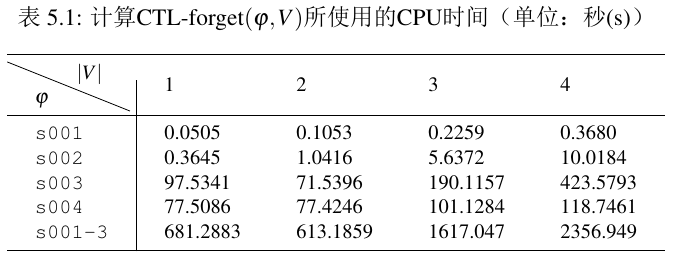
\includegraphics[scale=0.35]{figures/expTab}
%			\caption{
%				标准数据集来源于$\CTL$-RP:\\ \url{https://sourceforge.net/projects/ctlrp/}}
		\end{figure}
%		\begin{block}{实验结果}
%			标准数据集来源于$\CTL$-RP\footnote{\url{https://sourceforge.net/projects/ctlrp/}}
%%			\begin{table}%[width=.9\linewidth,cols=4,pos=h]
%%				\small
%%				\centering
%%				\caption{计算 {\CTL-forget}$(\varphi, V)$所使用的CPU时间(单位:秒(s))}\label{chapter04:tab:sample}
%%				\setlength{\tabcolsep}{5mm}{
%%					\begin{tabular}{l|llll}%{@{} L|LLLL@{} }
%%						\toprule
%%						%\diagbox[width=6em]{$\varphi$}{$|V|$}&
%%						$\varphi$, $|V$ & 1        & 2       & 3        & 4   \\
%%						\midrule
%%						\texttt{s001}         & 0.0505 & 0.1053 & 0.2259 & 0.3680 \\ 
%%						\texttt{s002}         & 0.3645          & 1.0416          & 5.6372          & 10.0184          \\ 
%%						\texttt{s003}         & 97.5341          & 71.5396          & 190.1157          & 423.5793          \\ 
%%						\texttt{s004}         & 77.5086          & 77.4246          & 101.1284          & 118.7461          \\ 
%%						\texttt{s001-3} & 681.2883   & 613.1859 & 1617.047 & 2356.949 \\
%%						\bottomrule
%%				\end{tabular}}
%%			\end{table}
%		\end{block}

(2) 计算{\CTL-forget}$(\varphi, V)$使用的时间和在“移除原子命题”步骤后$\CTLsnf$子句的个数,其中$\varphi=\varphi_1 \wedge \ALL\NEXT \varphi_2 \wedge \EXIST\NEXT \varphi_3$,$\varphi_i=12~(i=1,2,3)$。

	\begin{figure}
		\centering
		\subfigure[{\scriptsize 计算遗忘需要的CUP时间}]{
			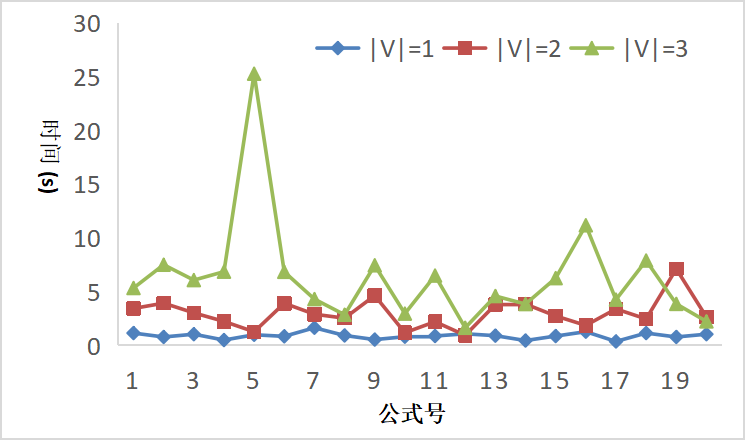
\includegraphics[scale=0.3]{figures/time_4_12_2.png}
		}\qquad
		\subfigure[{\scriptsize $\CTLsnf$子句的个数}]{
			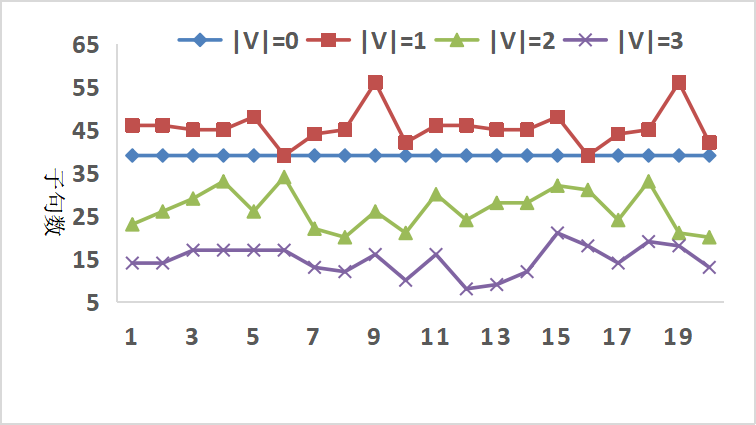
\includegraphics[scale=0.3]{figures/number-4-12_2.png}
		}
	%	\caption{计算{\CTL-forget}$(\varphi, V)$使用的时间和在“移除原子命题”步骤后$\CTLsnf$子句的个数,其中$\varphi_i=12$。$$\varphi=\varphi_1 \wedge \ALL\NEXT \varphi_2 \wedge \EXIST\NEXT \varphi_3$$}
		\label{chapter04:fig:for12}
	\end{figure}
	} 
\end{frame}


\begin{frame}
	\frametitle{研究内容(三)(3)算法CTL-forget实验——{\footnotesize 实验 2:计算SNC}}
	{\footnotesize
		\textcolor{blue!60}{计算$q$在$V$和$\varphi \wedge q$上的SNC($\CTLforget(\varphi\wedge q, \Var(\varphi)-V \cup \{q\})$),其中$V\subseteq \Var(\varphi)$、$q\in \Var(\varphi\wedge q)-V$。}
		
%	\only<1>{(1)	随机3-CNF,$|\Ha|=50$,每组20个公式。
%		\begin{figure}
%		\centering
%		\subfigure[{\scriptsize 平均CPU时间(s)}]{
%			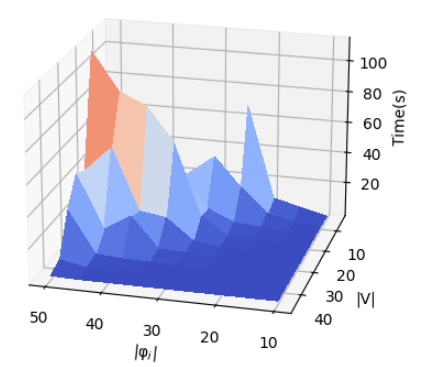
\includegraphics[scale=0.3]{figures/PRototalAveTime2.png}
%		}\qquad
%		\subfigure[{\scriptsize $|V|=25$时所使用CPU时间箱线图}]{
%			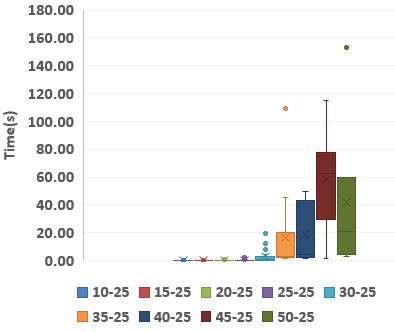
\includegraphics[scale=0.3]{figures/ProBox(10-50)_25_2.png}
%		}
%		\caption{{\footnotesize 计算3-CNF公式SNC的CPU时间}}
%	\end{figure}
%}
%		\only<2>{	
%		(2) 
		$\CTL$公式$\varphi=\varphi_1 \wedge \ALL\NEXT \varphi_2 \wedge \EXIST\NEXT \varphi_3$,$\varphi_i=12~(i=1,2,3)$为$|\Ha|=50$上的3-CNF且$|\varphi_1|=|\varphi_2|=|\varphi_3|$,每组40个公式。
		
		\begin{figure}
			\centering
			\subfigure[{\scriptsize 平均CPU时间(s)}]{
				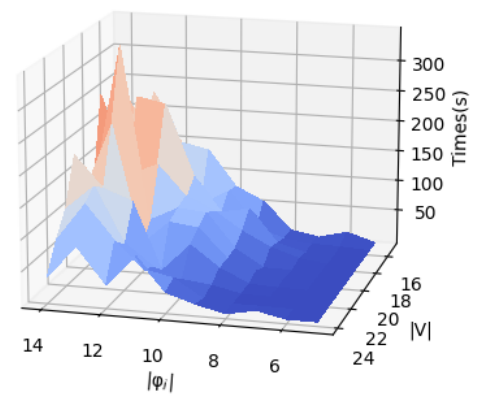
\includegraphics[scale=0.3]{figures/totalAveTime1.png}
			}\qquad
			\subfigure[{\scriptsize 存在SNC的公式占比(\%)}]{
				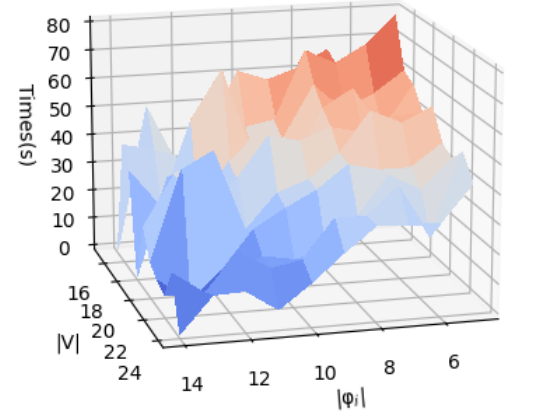
\includegraphics[scale=0.3]{figures/numPercent1.png}
			}
		\caption{{\footnotesize 计算$\CTL$SNC的平均时间和存在SNC的公式占比}}
		\end{figure}
%	}
\pause
\textcolor{red}{\textbf{总结:}基于归结的算法大多数情况下能计算出SNC(WSC),且当需要遗忘的原子个数很少或公式长度较小时计算效率较高。}
	}
\end{frame}


	
	\section{总结与展望}
	\subsection*{总结}
	\begin{frame}
		\frametitle{~~总结}
		\begin{itemize}[<+-| alert@+>]
			\vskip 8pt
			\item $\CTL$和$\mu$-演算的遗忘理论
			\begin{itemize}
				\item $\CTL$的遗忘理论:基本性质(表达性理论、代数属性和封闭性等)
				\item $\mu$-演算的遗忘理论:基本性质、复杂性和互模拟不变性等
			\end{itemize}
			\item 遗忘理论在反应式系统的形式化验证和知识更新中的应用
			\begin{itemize}
				\item 计算WSC和SNC:定义、基本性质和基于遗忘的计算方法等
				\item 定义知识更新:两种知识更新定义和基本性质
			\end{itemize}
			\item 计算$\CTL$遗忘的算法
			\begin{itemize}
				\item 基于模型的计算方法:有界互模拟、特征值、特征公式、封闭性、复杂性和算法等
				\item 基于消解(resolution)的计算方法:算法及其可靠性、遗忘存在的子类
				\item 实现与实验分析
			\end{itemize}
		\end{itemize}
	\end{frame}
	
	\subsection*{展望}
	\begin{frame}
		\frametitle{~~展望}
	%	\text{\Large 展望:} 
		\begin{spacing}{1.5}
			\begin{itemize}
				\item CTL和$\mu$-演算的遗忘
					\begin{itemize}
						\item 遗忘结果总是存在的子类;
						\item 遗忘相关问题复杂性分析;
						\item CTL和$\mu$-演算遗忘之间的关系。
					\end{itemize}
				\item “CTL和$\mu$-演算公式的遗忘结果是否分别是CTL和$\mu$-演算可表示”这一问题的可判定性研究
				\item 遗忘与WSC(SNC)之间的相互关系与应用
			\end{itemize}
		\end{spacing}
	\end{frame}
	
	\begin{frame}
		\frametitle{~~参与项目及成果}
		\text{\Large 作者在攻读博士学位期间参与项目及成果} 
		\begin{spacing}{1.5}
			\begin{itemize}
				\item 发表文章
				\begin{itemize}
					\item 发表了一篇CCF B类会议;
					\item 两篇SCI论文在审。
				\end{itemize} 
				\item 参与项目
				\begin{itemize}
					\item 国家自然科学基金重点项目:数据共享应用的块数据融合分析理论与安全管控模型研究,项目基金号 U1836205;
				%	\item  国家自然科学基金:不完全知识的遗忘理论研究及应用,项目基金号;
					\item 国家自然科学基金:析取逻辑程序归纳学习研究及应用,项目基金号 61976065。
				\end{itemize} 
			\end{itemize}
		\end{spacing}
	\end{frame}
	
	\begin{frame}
		\centering{
		\zihao{2} 敬请各位专家批评指正}\\
		\[
		\zihao{1}\hbox{\textcolor{blue}{谢谢!}}
		\]
	\end{frame}

\begin{frame}[allowframebreaks] %allowramebreaks 可自动分页
	\frametitle{参考文献}
	%\nocite{*}
	\printbibliography[title=参考文献]
	%\bibliographystyle{alpha}
	%此文件虽然在chapters文件夹下,但是实际运行应该是在main.tex中,所以提取bib文件的路径要尤其注意。
	%\bibliography{paper}
\end{frame}

\appendix

\section{背景知识}
\subsection{Kripke结构}
\begin{frame}
	\frametitle{~Kripke结构}
	{\footnotesize	
		$\Ha$:原子命题的集合 \qquad \qquad $\Ind$:索引的集合
		\begin{definition}[初始$\Ind$-Kripke结构]
			一个初始$\Ind$-Kripke结构是一个五元组$\Hm=(S,R,L,$ $[\_],s_0)$,其中:
			\begin{itemize}
				\item $S$是状态的非空集合,$s_0$是$\Hm$的初始状态(参见下文);
				\item $R \subseteq S \times S$是状态转换函数,且对任意$s\in S$,存在$s'\in S$使得$(s,s') \in R$;
				\item $L:S\rto 2^{\Ha}$是一个标签函数;
				\item $[\_]: \Ind \rto 2^{S \times S}$是一个函数,其使得对任意$ind \in\Ind$,若$s\in S$,则存在唯一一个$s\in S$使得$(s,s')\in [ind]\cap R$。
			\end{itemize}
		\end{definition}
		%	\only<1>{\begin{block}{相关概念}
		%		\begin{itemize}
		%			\item 初始Kripke结构$\Hm=(S,R,L,s_0)$:从初始$\Ind$-Kripke结构$\Hm$中去掉$[\_]$元素得到;
		%			\item $\Ind$-Kripke结构$\Hm=(S,R,L,[\_])$:从初始$\Ind$-Kripke结构$\Hm$中去掉初始状态$s_0$得到;
		%			\item Kripke结构$\Hm=(S,R,L)$:从初始$\Ind$-Kripke结构$\Hm$中同时去掉$[\_]$和$s_0$得到。
		%		\end{itemize}
		%	\end{block}}
		%	\only<2>{
		%		\begin{block}{相关概念}
		%			令$\Hm=(S,R,L)$为Kripke结构,$\Hm'=(S,R,L, [\_])$为$\Ind$-Kripke结构 :
		%			\begin{itemize}
		%				\item 路径:$\Hm$上的{\em 路径}是$\Hm$上的状态构成的无限序列$\pi=(s_0, s_{1}, s_{2},\dots)$,且满足对任意$j\ge 0$,$(s_j, s_{j+1}) \in R$;
		%				\item $s'\in \pi$:表示$s'$是路径$\pi$上的一个状态;  $\pi_{s}$:表示以$s$为起点的$\Hm$上的一条路径;
		%				\item 初始状态:如果对任意$s'\in S$,都存在路径$\pi_{s}$使得$s'\in \pi_{s}$,那么称$s$为\emph{初始状态};
		%				\item 索引路径:$\Hm'$上的一条\emph{索引路径}$\pi_{s}^{\tuple{ind}}$($ind \in \Ind$)是一条路径$(s_0(=s),$ $s_{1},$ $s_{2},$ $\dots)$,且对任意$j \geq 0$,有$(s_j, s_{j+1}) \in [ind]$。
		%			\end{itemize} 
		%		\end{block}
		%	}
		%	\only<3>{
		\begin{block}{相关概念}
			\begin{itemize}
				\item \textcolor{blue!80}{($\Ind$-)结构}:初始($\Ind$-)Kripke结构$\Hm$和是$\Hm$中的状态$s$构成的二元组${\cal K}=(\Hm, s)$;
				\item \textcolor{blue!80}{初始 ($\Ind$-)结构}:($\Ind$-)结构${\cal K}=(\Hm, s)$中$s$为初始状态的情形。
			\end{itemize} 
			
			%	在这些结构中,(索引)路径这一概念可以类似地定义。
		\end{block}
		%	}
	}
\end{frame}


\subsection{CTL的语法和语义}
\begin{frame} 
	\frametitle{~$\CTL$的语法}
	{\footnotesize 
		%	\only<1>{
		\begin{block}{$\CTL$的语言符号}
			\begin{itemize}
				\item 原子命题集$\Ha$; \quad 可数无限索引集合$\Ind$;\quad 命题常量$\start$;
				\item 常量符号:$\top$和$\bot$,分别表示“真”和“假”;
				\item 联结符号:$\vee$和$\neg$,分别表示“析取”和“否定”;
				\item 路径量词:$\ALL$、$\EXIST$和$\EXIST_{ind}$,分别表示“所有”、“存在”和“存在索引为$ind\in \Ind$”的路径;
				\item 时序操作符:$\NEXT$、$\FUTURE$、$\GLOBAL$、$\UNTILL$和$\UNLESS$,分别表示“下一个状态”、“将来某一个状态”、“将来所有状态”、“直到”和“除非”;
				\item 标点符号:“(”和“)”。
			\end{itemize}
		\end{block}
		%}
		\begin{definition}[带索引的$\CTL$]
			带索引的$\CTL$公式的\emph{存在范式(existential normal form, ENF)}可以用巴科斯范式递归定义如下:
			\begin{align*}
				\phi  ::= & \ \start\mid \bot %\mid \top
				\mid p \mid\neg\phi \mid \phi\lor\phi \mid
				\EXIST \NEXT \phi \mid
				\EXIST \GLOBAL \phi \mid 
				\EXIST (\phi\ \UNTILL\ \phi)\mid 
				\EXIST_{\tuple{ind}}\NEXT \phi  \mid 
				\EXIST_{\tuple{ind}}\GLOBAL \phi \mid
				\EXIST_{\tuple{ind}}(\phi \UNTILL \phi)  
			\end{align*}
			其中,$p\in \Ha$,$ind \in \Ind$。
			
			\textcolor{blue}{没有索引和$\start$的公式称为$\CTL$公式。}
		\end{definition} 
	}
\end{frame}

\begin{frame} 
	\frametitle{~$\CTL$的语义}
	{\footnotesize  
		\begin{definition}[带索引的$\CTL$的语义]\label{def:ctl:semantic}
			给定公式$\varphi$,初始$\Ind$-Kripke结构 $\Hm=(S,R,L,[\_],s_0)$ 和状态 $s\in S$。$(\Hm,s)$与$\varphi$之间的可满足关系$(\Hm,s)\models \varphi$定义如下:
			\begin{figure}
				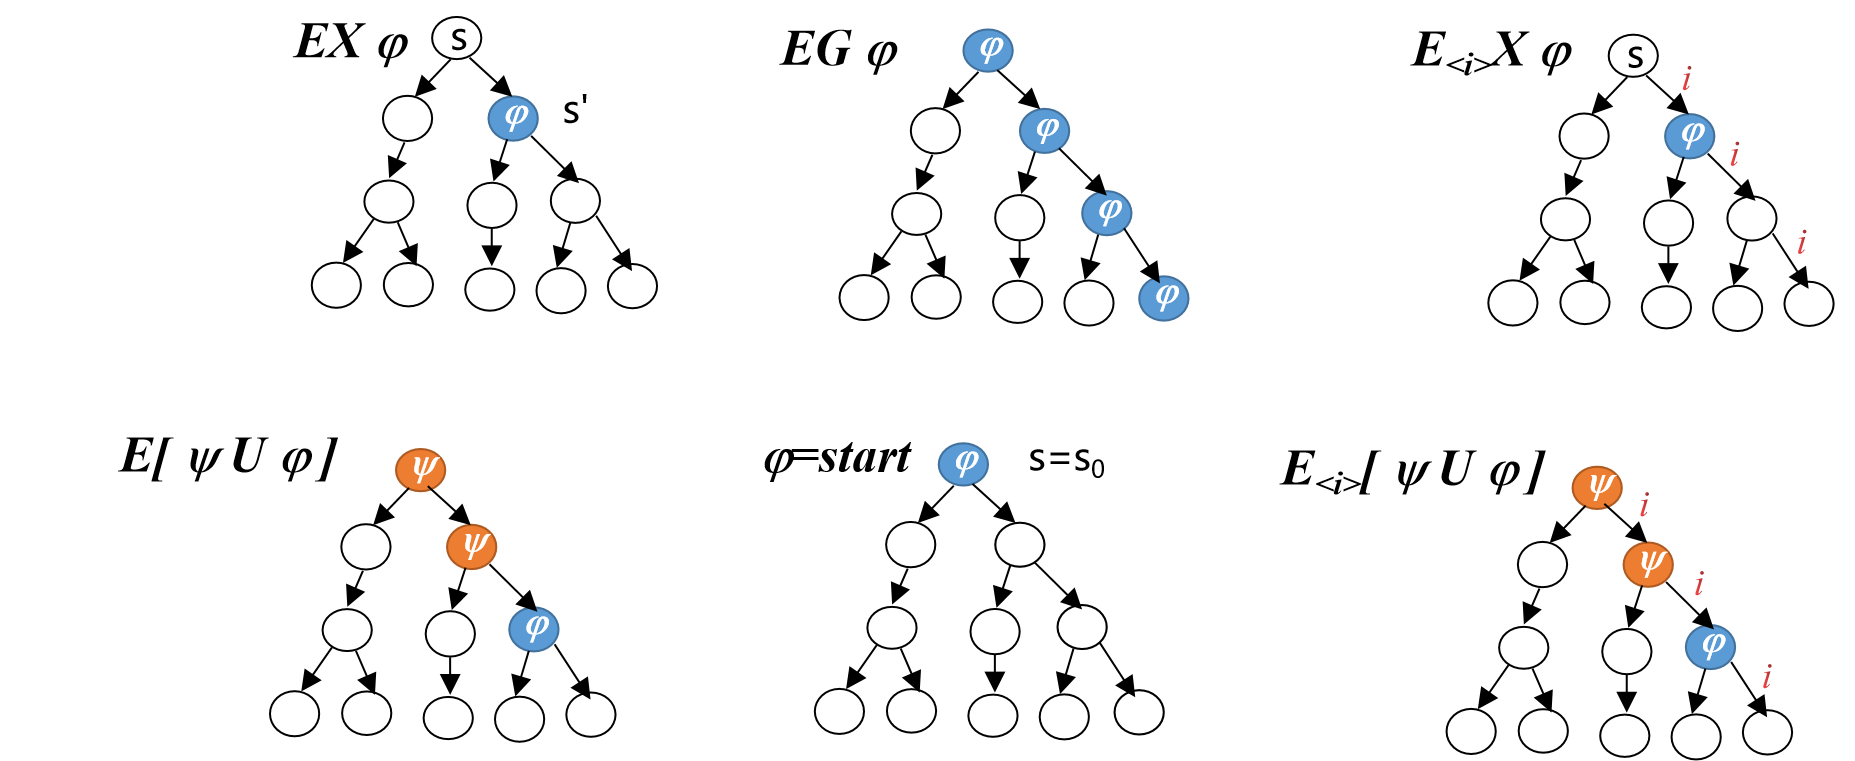
\includegraphics[scale=0.3]{figures/semanticCTL}
			\end{figure}
		\end{definition}%\pause
		\begin{block}{{\footnotesize 小贴士}}
			\tiny{
				\begin{itemize}
					\item \textcolor{blue!80}{模型}:满足公式$\varphi$的初始$\Ind$-结构称为$\varphi$的一个模型;\qquad $\Mod(\varphi)$:公式$\varphi$的所有模型构成的集合; 
					%\item 
					\item \textcolor{blue!80}{$\IR(\varphi,V)$}:如果存在一个公式$\psi$使得$\Var(\psi) \cap V = \emptyset$且$\varphi \equiv \psi$,则说$\varphi$与$V$中的原子命题\textcolor{blue!80}{无关},简称为\textcolor{blue!80}{$V$-无关};\\ $\Var(\varphi)$:出现在$\varphi$中的原子命题集;
					\item 可满足、逻辑蕴涵、逻辑等值、文字、子句等跟经典命题情形中的定义一样。
				\end{itemize}
			}
		\end{block} 
	}
\end{frame}


\begin{frame} 
	\frametitle{~$\CTL$的标准形式}
	{\footnotesize 
		\only<1>{\begin{block}{$\CTLsnf$子句}
				具有下面几种形式的公式称为$\CTL$全局子句分离范式(separated normal form with global clauses for \CTL,$\CTLsnf$子句)\cite{zhang2008first,zhang2014resolution}:
				\[
				\begin{array}{ll}
					\textcolor{blue!80}{\ALL \GLOBAL} (\start \rto \bigvee_{j=1}^{k} m_{j}) & \text{(初始句,initial clause)} \\
					\textcolor{blue!80}{\ALL \GLOBAL} (\top\rto \bigvee_{j=1}^{k} m_{j}) &\text{(全局子句,global clause)} \\
					\textcolor{blue!80}{\ALL \GLOBAL} (\bigwedge_{i=1}^{n} l_{i} \rto \ALL \NEXT \bigvee_{j=1}^{k} m_{j}) & (\ALL\text{-步子句,} \ALL\text{-step clause}) \\
					\textcolor{blue!80}{\ALL \GLOBAL} (\bigwedge_{i=1}^{n} l_{i} \rto \EXIST_\tuple{ind} \NEXT \bigvee_{j=1}^{k} m_{j}) & (\EXIST\text{-步子句,} \EXIST\text{-step clause}) \\
					\textcolor{blue!80}{\ALL \GLOBAL} (\bigwedge_{i=1}^{n} l_{i} \rto \ALL \FUTURE l) & (\ALL\text{-某时子句,} \ALL\text{-sometime clause}) \\
					\textcolor{blue!80}{\ALL \GLOBAL} (\bigwedge_{i=1}^{n} l_{i} \rto \EXIST_{\tuple{ind}} \FUTURE l) & (\EXIST\text{-某时子句,} \EXIST\text{-sometime clause})\\
				\end{array}
				\]
				其中$k$和$n$都是大于0的常量,$l_i$($1\leq i \leq n$)、$m_j$($1\leq j \leq k$)和$l$都是文字且$ind \in \Ind$。
		\end{block}}
		\only<2>{
			\begin{block}{转换规则}
				一个$\CTL$公式$\varphi$可以通过下表中的规则转换为一个$\CTLsnf$子句集,记为$T_{\varphi}$。 
				{\tiny
					\begin{table}%[width=.9\linewidth,cols=4,pos=h] 
						\centering 
						\caption{{\scriptsize 转换规则}}\label{tab:trans} 
						\begin{tabular}{c}
							\toprule
							$
							\begin{aligned}
								& \textbf{Trans(1)}\frac{q \rto \EXIST T \varphi}{q\rto \EXIST_{\tuple{ind}} T \varphi}; \qquad
								\textbf{Trans(2)} \frac{q \rto \EXIST (\varphi_1 \UNTILL \varphi_2)}{q\rto \EXIST_{\tuple{ind}} (\varphi_1 \UNTILL \varphi_2)};
								&& 
								\textcolor{red}{\textbf{Trans(3)} \frac{q\rto \varphi_1 \wedge \varphi_2}{q\rto \varphi_1, q\rto \varphi_2};}\\
								&   \textbf{Trans(4)}  \frac{q\rto \varphi_1 \vee \varphi_2\ (\hbox{如果$\varphi_2$不是子句})}{ q\rto \varphi_1 \vee p, p\rto \varphi_2};
								&&\textbf{Trans(5)}  \frac{q\rto D}{\top \rto \neg q \vee D};\ \frac{q\rto \perp}{ \top \rto \neg q};\ \frac{q \rto \top}{\{\}} \\
								&  \textbf{Trans(6)} \frac{q\rto Q\NEXT \varphi\ (\hbox{如果$\varphi$不是子句})}{q\rto Q\NEXT p, p\rto \varphi}; 
								&& \textbf{Trans(7)} \frac{q\rto Q\FUTURE \varphi\ (\hbox{如果$\varphi$不是文字})}{q\rto Q\FUTURE p, p\rto \varphi}; \\
								&  \textbf{Trans(8)} \frac{q\rto Q(\varphi_1 \UNTILL \varphi_2) \  (\hbox{如果$\varphi_2$不是文字})}{q\rto Q(\varphi_1 \UNTILL p),  p\rto \varphi_2}; 
								&& \textbf{Trans(10)} \frac{q\rto Q\GLOBAL \varphi}{\ q \rto  p, p\rto \varphi,p\rto Q\NEXT p};\\
								& \textbf{Trans(9)} \frac{q\rto Q(\varphi_1 \UNLESS \varphi_2)\ (\hbox{如果 $\varphi_2$ 不是文字})}{q\rto Q(\varphi_1 \UNLESS p), p\rto \varphi_2}; &&\\  
								& \textbf{Trans(11)} \frac{q\rto Q(\varphi \UNTILL l)}{q \rto l\vee p, p\rto \varphi, p\rto Q\NEXT(l\vee p),q\rto Q \FUTURE l};
								&& \textbf{Trans(12)} \frac{q\rto Q(\varphi \UNLESS l)}{q \rto l\vee p, p\rto \varphi, p\rto Q\NEXT(l\vee p)}.
							\end{aligned}
							$\\
							\bottomrule
						\end{tabular}
				\end{table}}
				其中,$T\in \{\NEXT, \GLOBAL, \FUTURE\}$,$ind$是规则中引入的新索引且$Q\in \{\ALL, \EXIST_{\tuple{ind}}\}$;
				$q$是一个原子命题, $l$是一个文字, $D$是文字的析取(即子句), $p$是新的原子命题;$\varphi$,$\varphi_1$,和$\varphi_2$都是$\CTL$公式。
			\end{block}
		} 
	}
\end{frame}

\begin{frame}
	\frametitle{~$\CTL$的标准形式}
	\begin{example}\label{examp:Tran}
		\tiny
		令$\varphi=\neg \ALL \FUTURE p \wedge \ALL\FUTURE(p \wedge \top)$,下面给出将$\varphi$转换为$\CTLsnf$子句集的详细步骤。
		
		(1) 将公式$\varphi$转换为其NNF形式:$\EXIST\GLOBAL \neg p \wedge \ALL\FUTURE(p \wedge \top)$;
		
		(2) 化简(1)中的公式为:$\EXIST\GLOBAL \neg p \wedge \ALL\FUTURE p$;
		
		(3) 使用转换规则转换$\{\ALL\GLOBAL(\start \rto z), \ALL\GLOBAL(z \rto (\EXIST\GLOBAL \neg p \wedge \ALL\FUTURE p))\}$,详细步骤如下:
		\begin{align*}
			&1.\ \start \rto z && \\
			&2.\ z \rto \EXIST\GLOBAL \neg p \wedge \ALL\FUTURE p &&  \\
			% \end{align*}
			% \begin{align*}
			& 3.\ \boxed{z \rto  \EXIST\GLOBAL \neg p} && (2, \textcolor{red}{\textbf{Trans(3)}})\\
			&4.\ \boxed{z \rto \ALL\FUTURE p} && (2, \textcolor{red}{\textbf{Trans(3)}})\\
			&5.\ z \rto  \EXIST_{\tuple{1}}\GLOBAL \neg p  && (3, \textbf{Trans(1)})\\
			&6.\ z \rto x && (5, \textbf{Trans(10)})\\
			&7.\ x\rto \neg l && (5, \textbf{Trans(10)})\\
			&8.\ x\rto \EXIST_{\tuple{1}} \GLOBAL x&& (5, \textbf{Trans(10)})\\
			&9.\ \top \rto \neg z \vee x && (6, \textbf{Trans(5)}) \\
			% \end{align*}
			% \begin{align*}
			&10.\ \top \rto \neg x \vee \neg p && (7, \textbf{Trans(5)}) 
		\end{align*}
		
		因此,得到的$\varphi$对应的$\CTLsnf$子句集为:
		\begin{align*}
			&1.\ \start \rto z && 2.\ z \rto \ALL\FUTURE p && 3.\ x\rto \EXIST_{\tuple{1}} \GLOBAL x
			&& 4.\ \top \rto \neg z \vee x && 5.\ \top \rto \neg x \vee \neg p.
		\end{align*}
	\end{example}
\end{frame}

\subsection{$\mu$-演算}
\begin{frame} 
	\frametitle{~$\mu$-演算的语法和语义}
	{\footnotesize 
		不动点符号:$\mu$和$\nu$;\qquad
		${\cal V}$:变元符号的可数集。 
		\begin{definition}[$\mu$-演算公式]
			$\mu$-演算公式(简称为$\mu$-公式或公式)递归定义如下:
			\[
			\varphi ::=   p\mid  X\mid \neg \varphi\mid \varphi \vee \varphi \mid \ALL\NEXT \varphi\mid  \nu X. \varphi
			\]
			其中$p\in \Ha$且$X\in {\cal V}$。
		\end{definition}
		\begin{definition}
			给定$\mu$-演算公式$\varphi$、Kripke结构{\em $\Hm=(S,R,L,r)$}和一个从${\cal V}$中的变量到$\Hm$中状态的赋值函数$v: {\cal V} \rto 2^S$。公式在$\Hm$和$v$上的解释是$S$的一个子集$\left\| \varphi\right\|_v^{\Hm}$(如果在上下文中$\Hm$是明确的,则可以省去上标):
			\begin{columns}
				\column{0.5\textwidth}
				\begin{align*}
					& \left \| p\right \|_v^{\Hm} = \{s\mid p \in L(s)\}, \\  
					& \left\| X\right\|_v^{\Hm} = v(X),\\
					& \left\|\varphi_1 \vee \varphi_2\right\|_v^{\Hm} = \left\|\varphi_1\right\|_v^{\Hm} \cup \left\|\varphi_2\right\|_v^{\Hm},\\ 
					& \left\|\ALL \NEXT \varphi\right\|_v^{\Hm} = \{s\mid \forall s'. (s, s') \in R \Rto s' \in \left\|\varphi\right\|_v^{\Hm}\},\\ 
					& \left\| \nu X. \varphi\right\|_v^{\Hm} = \bigcup\{S' \subseteq S \mid S' \subseteq \left\|\varphi\right\|_{v[X:= S']}^{\Hm}\}.
				\end{align*}
				\column{0.5\textwidth}
				{\tiny 
					\begin{block}{{\scriptsize 小贴士}}
						\begin{itemize} 
							\item 赋值:$(\Hm,s,v)$,$(\Hm,v)$;
							\item 若$s\in \left\| \varphi \right\|_v$,则称$s$“满足”$\varphi$,记为$(\Hm, s, v) \models \varphi$;
							\item 这里的Kripke结构不要求其二元关系是完全的;
							\item 当公式$\varphi$为$\mu$-句子时,可以将赋值函数$v$省略;
							\item 范式:析取$\mu$-公式。
						\end{itemize}
					\end{block}
				} 
			\end{columns}
			
			其中,$v[X:= S']$是一个赋值函数,它除了$v[X:= S'](X)=S'$之外,和$v$完全相同。
		\end{definition}
		 
	}
\end{frame}

\section{研究内容(一):CTL和$\mu$-演算的遗忘理论}
\subsection{CTL遗忘理论}  
\begin{frame}  
	\frametitle{~CTL和$\mu$遗忘理论——{\footnotesize 总体框架}}
	\begin{figure}
		\includegraphics[scale=0.35]{figures/ctlMuForgFrame}
		\caption{CTL和$\mu$-演算遗忘理论}
	\end{figure}
\end{frame}

\begin{frame} 
	\frametitle{~CTL遗忘理论——{\footnotesize 互模拟}}
	{\scriptsize 
		\begin{definition}[$V$-互模拟]
			\label{def:VInd:bisimulation}
			给定原子命题集$V\subseteq\cal A$、索引集合$I\subseteq \Ind$和初始$\Ind$-结构 $\Hm_i=(S_i, R_i,L_i, [\_]_i, s_0^i)~(i=1,2)$。
			$\Hb_V \subseteq S_1 \times S_2$为二元关系,对任意$s_1 \in S_1$和$s_2 \in S_2$,若$(s_1, s_2)\in \Hb_V$,则:
			\begin{itemize}[<+-| alert@+>]
				\item[(i)] $L_1(s_1) - V = L_2(s_2) -V$;
				\item[(ii)] $\forall r_1\in S_1$, 若$(s_1, r_1)\in R_1$,则$\exists r_2 \in S_2$ 使得 $(s_2,r_2) \in R_2$ 和 $(r_1, r_2) \in \Hb_V$;
				\item[(iii)] $\forall r_2\in S_2$,若$(s_2, r_2)\in R_2$,则 $\exists r_1 \in S_1$ 使得 $(s_1,r_1) \in R_1$ 和 $(r_1, r_2)\in \Hb_V$。
			\end{itemize}
			那么,称 $\Hb_V$ 是 $\Hm_1$和 $\Hm_2$之间的一个 $V$-互模拟关系。
		\end{definition}
		%		\only<1>{
		\begin{columns}
			\column{0.5\textwidth} 
			\begin{itemize}
				\item \textcolor{blue!80}{结构互模拟}:若$\Hm_1$和 $\Hm_2$之间存在一个 $V$-互模拟关系$\Hb_V$使得$(s_1, s_2)\in \Hb_V$,则称两个 $\Ind$-结构 ${\cal K}_1$ $= (\Hm_1, s_1)$ 和 ${\cal K}_2 = (\Hm_2, s_2)$ 是 $V$-{\em 互模拟}的,记为${\cal K}_1$ $\lrto_V {\cal K}_2$;
				\item \textcolor{blue!80}{路径互模拟}:令$i\in \{1,2\}$,$\pi_i=(s_{i,1},$ $s_{i,2},\ldots)$ 为 $\Hm_i$ 上的路径,若对任意$j \ge 1$都有$ {\cal K}_{1,j} \lrto_V {\cal K}_{2,j}$,则称这两条路径是$V$-{\em 互模拟}的,记为$\pi_1 \lrto_V \pi_2$,其中 ${\cal K}_{i,j}=(\Hm_i,$ $s_{i,j})$。
			\end{itemize}
			\column{0.5\textwidth}
			\begin{figure}
				\centering
				\begin{tikzpicture}[scale=0.75]
					\tikzstyle{every node}=[font=\small,scale=0.75]
					\begin{minipage}{.2\textwidth}
						\node[blueCircle] (s0) at(0,1) {$s_0$};
						\node[blueCircle1] (s1) at(0,0) {$s_1$};
						\node[blueCircle3] (s2) at(-1,0) {$s_2$};
						\node[redCircle] (s3) at(1,0) {$s_3$};
						\node[redCircle] (s4) at(0.5,-1) {$s_4$}; 
						\draw[->,dashed] (s0) -- (s1);
						\draw[->,dashed] (s1) -- (s2);
						\draw[->,dashed] (s1) -- (s3);
						\draw[->,dashed] (s1) -- (s4);
						%	\draw[->] (s4) -- (s0);
						\path (s4) edge[->,bend right=45] (s0);
						\path (s2) edge[->,bend right=-45] (s0);
						\path (s3) edge[->,bend right=45] (s0);
						\node at(-0.2,1.3) {$d$};
						\node at(-1.4,0) {$se$};
						\node at(1.4,0) {$sp$};
						\node at(-0.3,-0.3) {$s$};
						\node at(-0.2,-1) {$se, sp$};
						\node at(-0.4, -0.6) {${\cal K}_1$};
					\end{minipage}
					\begin{minipage}{.2\textwidth}
						\node[blueCircle] (s10) at(3,2) {$s_0$};
						\node[blueCircle1] (s11) at(3,1) {$s_1$};
						\node[blueCircle2] (s12) at(2,1) {$s_2$};
						\node[redCircle] (s13) at(4,1) {$s_3'$};
						\draw[->] (s10) -- (s11);
						\draw[->] (s11) -- (s12);
						\draw[->] (s11) -- (s13);
						\path (s12) edge[->,bend right=-45] (s10);
						\path (s13) edge[->,bend right=45] (s10);
						%\draw[<->] (s0) -- (s12);
						\node at(2.8,2.3) {$d$};
						\node at(1.6,1.2) {$se$};
						\node at(4.4,1) {$\emptyset$};
						\node at(2.7,0.7) {$s$};
						\node at(2.6,0.4) {${\cal K}_2$};
					\end{minipage}
					\begin{minipage}{.2\textwidth}
						\node[blueCircle] (s20) at(3,-1) {$s_0$};
						\node[blueCircle1] (s21) at(3,-2) {$s_1$};
						\node[blueCircle3] (s22) at(2,-2) {$s_2'$};
						\draw[->] (s20) -- (s21);
						\draw[->] (s21) -- (s22);
						\path (s22) edge[->,bend right=-45] (s20);
						\node at(2.7,-0.7) {$d$};
						\node at(1.6,-2) {$\emptyset$};
						\node at(2.7,-1.4) {$s$};
						\node at(3.4,-2) {${\cal K}_3$};
					\end{minipage}
					\draw[<->,dashed] (s0) -- (s12);
					\node at(1,1.1) {{\tiny $\{j\}$-互模拟}};
					\draw[<->,dashed] (s11) -- (s20);
					\node at(3,0) {{\tiny $\{se\}$-互模拟}};
					\draw[<->,dashed] (s4) -- (s22);
					\node at(1,-1.5) {{\tiny $\{se,sp\}$-互模拟}};
					%	\node at(0,-1.5) {${\cal K}_2$}; 
				\end{tikzpicture}
				\caption{{\tiny 汽车制造企业模型}} 
			\end{figure}
			%			\begin{figure}
			%				\includegraphics[scale=0.34]{figures/NVBnewCar1}
			%			\end{figure}
		\end{columns}
		%}
		%	\only<2>{
		%	%	\begin{block}{相关性质 1} 
		%			\begin{proposition}
		%				给定集合$V_i\subseteq \Ha$、状态$s_i'$、路径$\pi_i'$和$\Ind$-结构${\cal K}_j=(\Hm_j,s_j)$,其中$i=1,2$,$j=1,2,3$。 
		%				如果${\cal K}_1 \lrto_{V_1} {\cal K}_2$且${\cal K}_2 \lrto_{V_2} {\cal K}_3$,则:
		%				\begin{itemize}
		%					\item[(i)] ${\cal K}_1\lrto_{V_1\cup V_2}{\cal K}_3$;
		%					\item[(ii)] 若 $V_1 \subseteq V_2$,则 ${\cal K}_1 \lrto_{V_2} {\cal K}_2$;
		%					\item[(iii)] $s_1'\lrto_{V_i}s_2'~(i=1,2)$ 蕴涵$s_1'\lrto_{V_1\cup V_2}s_2'$;
		%					\item[(iv)] $\pi_1'\lrto_{V_i}\pi_2'~(i=1,2)$ 蕴涵 $\pi_1'\lrto_{V_1\cup V_2}\pi_2'$;
		%					\item[(v)] 对$\Hm_1$上的每条路径 $\pi_{s_1}$,存在$\Hm_2$上的一条路径 $\pi_{s_2}$ 使得 $\pi_{s_1} \lrto_{V_1} \pi_{s_2}$,反之也成立。
		%				\end{itemize}
		%			\end{proposition}
		%	%	\end{block}
		%	}
		%	\only<2>{
		%		\begin{theorem}[互模拟不变性]\label{thm:V-bisimulation:EQ}
		%			令$V\subseteq \Ha$是原子命题集,${\cal K}_i$ $(i=1,2)$是两个具有$V$-互模拟关系的$\Ind$-结构,即:${\cal K}_1 \lrto_V {\cal K}_2$。若$\Phi$是一个$\CTL$公式且$\IR(\Phi, V)$,则有${\cal K}_1\models \Phi$当且仅当${\cal K}_2\models \Phi$。
		%		\end{theorem}
		%	}
	}
\end{frame}

\begin{frame}
	\frametitle{~CTL遗忘理论——{\footnotesize 互模拟等价}}
	{\footnotesize
		%			\begin{theorem}[互模拟不变性]\label{thm:V-bisimulation:EQ}
		%			令$V\subseteq \Ha$是原子命题集,${\cal K}_i$ $(i=1,2)$是两个具有$V$-互模拟关系的$\Ind$-结构,即:${\cal K}_1 \lrto_V {\cal K}_2$。若$\Phi$是一个$\CTL$公式且$\IR(\Phi, V)$,则有${\cal K}_1\models \Phi$当且仅当${\cal K}_2\models \Phi$。
		%		\end{theorem}\pause
		\begin{definition}[互模拟等价,bisimilar equivalence]\label{def:bisimular:equivalene}
			给定原子命题集$V\subseteq {\cal A}$,公式$\varphi$和$\psi$。若对任意${\cal K}\models \varphi$,都存在一个${\cal K}'\models\psi$,使得${\cal K}\lrto_V{\cal K}'$;且对任意${\cal K}'\models\psi$,都存在一个${\cal K}\models \varphi$,使得${\cal K}\lrto_V{\cal K}'$,则称公式$\varphi$和 $\psi$是 {\em $V$-互模拟等价的(bisimilar equivalence)},记为 $\varphi\equiv_V\psi$。
		\end{definition}
		%\pause
		%\begin{lemma}~\label{lem:eqR}
		%		对任意$V\subseteq\cal A$,  $\lrto_V$和 $\equiv_V$为等价关系。
		%	\end{lemma}
		%\only<2>{
		%	\begin{corollary}~\label{cor:eqbi}
		%		令 $V$、$V_1$、$V_2$ 为$\cal A$的子集,$\varphi$和 $\psi$为公式。
		%		\begin{itemize}
		%			\item[(i)] 若 $\varphi\equiv\psi$,则 $\varphi\equiv_V\psi$。
		%			\item[(ii)] 若$\varphi$ 和 $\psi$不包括索引,且 $\varphi\equiv_\emptyset\psi$, 则 $\varphi\equiv\psi$。
		%			\item[(iii)] 若 $\varphi\equiv_{V_i}\psi~(i=1,2)$,则 $\varphi\equiv_{V_1\cup V_2}\psi$。
		%			\item[(iv)] 若 $\varphi\equiv_{V_1}\psi$ 和 $V_1\subseteq V_2$,则 $\varphi\equiv_{V_2}\psi$。
		%		\end{itemize}
		%	\end{corollary}
		%}
		\pause
		\begin{proposition}\label{prop:transform:V:EQ}
			令 $\varphi$为一个$\CTL$公式。则$\varphi\equiv_UT_\varphi$,其中 $T_\varphi=\CTLsnf(\varphi)$和
			$U=\Var(T_\varphi)-\Var(\varphi)$。
		\end{proposition}
	}
\end{frame}

\begin{frame}
	\frametitle{~CTL遗忘理论——{\footnotesize 定义}}
	{\footnotesize 
		\begin{definition}[遗忘,forgetting]\label{def:V:forgetting}
			令$V$是$\Ha$的子集,$\Phi$是公式。如果公式$\psi$满足下面条件: 
			\begin{itemize}
				\item $\psi$与$V$中的原子命题无关(即:$\IR(\psi, V)$);
				\item $\Mod(\psi)=\{{\cal K}\mid {\cal K} \mbox{是一个初始$\Ind$-结构}, \exists {\cal K}'\in\Mod(\phi)\ \text{使得}\ {\cal K}'\lrto_V{\cal K}\}$。
			\end{itemize}  
			那么,称$\psi$为从$\Phi$中遗忘$V$后得到的结果,记为$\CTLforget(\phi,V)$。
		\end{definition}
		\only<1>{\begin{block}{遗忘理论公设}
				给定$\CTL$公式$\varphi$、$\varphi'=\CTLforget(\varphi, V)$、原子命题集$V\subseteq \Ha$和$\varphi'=\CTLforget(\varphi, V)$,$\CTL$下遗忘理论公设如下:
				\begin{itemize}
					\item[(\W)] 削弱:$\varphi \models \varphi'$;
					\item[(\PP)] 正支持:对任意与$V$无关的公式$\eta$,若$\varphi \models \eta$则$\varphi' \models \eta$;
					\item[(\NgP)] 负支持:对任意与$V$无关的公式$\eta$,若$\varphi \not \models \eta$则$\varphi' \not \models \eta$;
					\item[(\textbf{IR})] 无关性: $\IR(\varphi', V)$。
				\end{itemize}
		\end{block}}
	}
\end{frame}

\begin{frame}
	\frametitle{~CTL遗忘理论——{\footnotesize 相关性质}}
	{\footnotesize 
		\only<1>{
			\begin{theorem}[表达性定理,Representation Theorem]\label{thm:close} 
				给定$\CTL$公式$\varphi$和$\varphi'$,$V \subseteq \Ha$为原子命题集。 
				下面的陈述是等价的:
				\begin{itemize}
					\item[(i)] $\varphi' \equiv \CTLforget(\varphi, V)$,
					\item[(ii)] $\varphi'\equiv \{\phi \mid\varphi \models \phi \text{和} \IR(\phi, V)\}$,
					\item[(iii)] 若$\varphi$、$\varphi'$和$V$与(i)和(ii)中提到的符号相同,则公设(\W)、(\PP)、(\NgP)和(\textbf{IR})成立。
				\end{itemize}
			\end{theorem}
		}
		\only<2>{
			\begin{example}\label{exp:e1}
				令$p$和 $x$为两个不同的原子命题,$\varphi(p,x)$\footnote{$\varphi(p,x)$ 表示具有原子命题集$\Var(\varphi)=\{p,x\}$的公式。}为下面公式合取~\cite{Maksimova:JANCL:1991}:
				\begin{align*}
					&\ALL\GLOBAL(\neg x \wedge \neg \ALL \GLOBAL p \rto \neg \ALL \NEXT \neg x),
					\qquad \ALL\GLOBAL(\neg \ALL\NEXT \neg x \rto \ALL \NEXT x),\\
					& \ALL\GLOBAL(\ALL\NEXT x \rto \neg x \wedge \neg \ALL \GLOBAL p),
					\qquad \ALL\GLOBAL(x \rto \neg \ALL\GLOBAL p),
					\qquad \ALL\GLOBAL(\ALL \FUTURE \ALL \GLOBAL p).
				\end{align*}
				Maksimova证明了$\varphi(p,x)\land \varphi(p,y)\models x\lrto y$,且不存在$\CTL$公式 $\psi$使得 $\Var(\psi)=\{p\}$且$\varphi(p,x)$ $\models x\lrto \psi$,即$\CTL$不具有Beth性质。
			\end{example}
			%	}
			%	\only<2,3>{
			\begin{proposition}\label{pro:uniforget}
				$\CTLforget(x\land \varphi(p,x), \{x\})$ 在 $\CTL$中是不可表示的。
			\end{proposition}
			\begin{theorem}\label{thm:PL:CTL}
				给定一个命题公式$\varphi$和原子命题集$V\subseteq \Ha$,则下面逻辑等式成立。
				\[\CTLforget(\varphi, V) \equiv \Forget(\varphi,V).
				\]
			\end{theorem}
		}
		\only<3>{
			%	\begin{lemma}\label{lem:KF:eq}
			%		给定两个公式$\varphi$和$\alpha$,原子命题$q \not \in (\Var(\varphi) \cup \Var(\alpha))$,则:$$\CTLforget(\varphi \wedge (q \lrto \alpha), q)\equiv \varphi.$$
			%	\end{lemma}
			\begin{proposition}[分解性,Decomposition]\label{disTF}
				对于给定的公式$\varphi$,原子命题集$V$,和原子命题$p$($p\not \in V$),下面的结论成立:
				\begin{itemize}
					\item $\CTLforget(\varphi,\{p\}\cup V) \equiv \CTLforget(\CTLforget(\varphi,p),V)$;
					\item $	\CTLforget(\varphi,V_1\cup V_2) \equiv \CTLforget(\CTLforget(\varphi,V_1),V_2)$.
				\end{itemize} 
			\end{proposition}
			\begin{proposition}[同质性]\label{pro:ctl:forget:2}
				令${\cal T} \in \{\NEXT, \FUTURE, \GLOBAL\}$、${\cal P} \in \{\ALL, \EXIST\}$,$\phi$为$\CTL$公式,且$P\subseteq\cal A$为原子命题集,则:
				$$\CTLforget({\cal P}{\cal T}\phi,P)\equiv {\cal P}{\cal T} \CTLforget(\phi,P).$$
			\end{proposition}
		}
	}
\end{frame}

\begin{frame}
	\frametitle{$\mu$-演算遗忘理论——{\footnotesize 变元-命题-互模拟}}
	{\footnotesize
		%	$\Hm_i = (S_i, R_i,L_i, r_i)~(i=1,2)$.
		\only<1>{\begin{definition}[$V$-互模拟]\label{def:VB}
				给定原子命题集$V \subseteq \Ha$和两个Kripke结构$\Hm_1$和 $\Hm_2$,其中$\Hm_i = (S_i, R_i,L_i, r_i)~(i=1,2)$。若$\Hb\subseteq S_1 \times S_2$满足下面几个条件:
				\begin{itemize}
					\item \fbox{\textcolor{red}{$r_1 \Hb r_2$,}}
					\item 对任意$s\in S_1$和 $t\in S_2$,若$s \Hb t$,则对任意$p \in \Ha- V$,有$p \in L_1(s)$当且仅当 $p \in L_2(t)$,
					\item 若$(s, s')\in R_1$和 $s \Hb t$,则存在一个 $t'$,使得$s' \Hb t'$和 $(t, t')\in R_2$,且
					\item 若 $s \Hb t$和$(t, t')\in R_2$,则存在一个$s'$,使得$(s, s')\in R_1$和 $t' \Hb s'$。
				\end{itemize}
				则称$\Hb$是$\Hm_1$和 $\Hm_2$的$V$-互模拟关系。
				
				$\Hm_1 \lrto_V \Hm_2$、$(\Hm_1,$ $r_1) \lrto_V (\Hm_2,r_2)$:如果$\Hm_1$和 $\Hm_2$之间存在一个$V$-互模拟关系。
			\end{definition}
			%	如果$\Hm_1$和 $\Hm_2$之间存在一个$V$-互模拟关系,那么${\cal B}$则称这两个Kripke结构$\Hm_1$和 $\Hm_2$及由这两个Kripke结构构成的结构$(\Hm_1,r_1)$和$(\Hm_2,r_2)$是$V$-互模拟的,分别记为$\Hm_1 \lrto_V \Hm_2$和$(\Hm_1,$ $r_1) \lrto_V (\Hm_2,r_2)$。
		}
		\only<2>{
			\begin{example}[不变性反例]\label{ex:2}
				令$\varphi=\ALL\NEXT \neg X \lor \ALL \NEXT X$,$(\Hm,v)$和 $(\Hm',v')$为赋值,其中$\Hm=(S,r,R,L)$、$\Hm'=(S',r',R',L')$且
				\begin{align*}
					& S=\{r, r_1\}, R=\{(r,r_1)\}, L(r) = L(r_1) = \emptyset, v(X) = \{r_1\},\\
					& S'=\{r', r_1',r_2'\}, R'=\{(r',r_1'),(r',r_2')\}, L(r') = L(r_1') = L(r_2')=\emptyset, v'(X) = \{r_1'\}.
				\end{align*}
				$\Hb=\{(r, r'), (r_1, r_1'), (r_1,r_2')\}$是$\Hm$和$\Hm'$之间的一个 $\emptyset$-互模拟。
				
				但是,\fbox{$(\Hm,v) \models \varphi$而$(\Hm',v') \not \models \varphi$}。 
				\begin{figure}
					\includegraphics[scale=0.35]{figures/counterEVBmu}
				\end{figure} 
			\end{example}
		}
		\only<3>{
			\begin{definition}[变元-命题-互模拟]
				给定$V \subseteq \Ha$、${\cal V}_1 \subseteq {\cal V}$、$\Hm_i = (S_i, r_i, R_i, L_i)$为Kripke结构、 $s_i\in S_i$且
				$v_i: {\cal V} \rto 2^{S_i}$,其中$i\in\{1,2\}$。若关系$\Hb\subseteq S_1 \times S_2$满足:
				\begin{itemize}
					\item $(s_1,s_2)\in\Hb$,
					\item $\Hb$是$\Hm_1$ 和$\Hm_2$之间的$V$-互模拟,且
					\item \textcolor{red}{对任意$(t_1,t_2)\in \Hb$和$X  \in {\cal V}-{\cal V}_1$,$t_2\in v_2(X)$当且仅当$t_1 \in v_1(X)$。}
				\end{itemize}	
				则称$\Hb$是$(\Hm_1,s_1, v_1)$ 和$(\Hm_2,s_2, v_2)$之间的一个{\em $\tuple{{\cal V}_1, V}$-互模拟}。
			\end{definition}
			%	\begin{itemize}
			%		\item {\em $(\Hm,s, v)\lrto_\tuple{{\cal V}_1, V} (\Hm',s',v')$}:若$(\Hm,s, v)$和$(\Hm',s',v')$之间存在一个$\tuple{{\cal V}_1, V}$-互模拟关系$\Hb$,则称$(\Hm,s, v)$和$(\Hm',s',$ $v')$是$\tuple{{\cal V}_1, V}$-互模拟的;
			%		\item 若$s=r$ 且$s'=r'$,则$(\Hm, s,v) $ $\lrto_{\tuple{{\cal V}_1, V}} (\Hm',s',v')$简写为$(\Hm, v) \lrto_{\tuple{{\cal V}_1, V}} (\Hm',v')$;
			%		\item $\tuple{{\cal V}_1, V}$是一个等价关系。
			%%		\item {\em Var-$V_1$-互模拟}:若$(\Hm,s, v)$和$(\Hm',s',v')$之间存在一个$\tuple{\emptyset, V_1}$-互模拟关系,则称$(\Hm,s, v)$和$(\Hm',s',v')$是{\em Var-$V_1$-互模拟的},记为$(\Hm, s,v) $ $\lrto_{V_1} (\Hm',s',v')$;称$\tuple{\emptyset, V_1}$-互模拟为Var-$V_1$-互模拟;
			%%		\item 若$s=r$ 且$s'=r'$,则$(\Hm, s,v) $ $\lrto_{\tuple{{\cal V}_1, V}} (\Hm',s',v')$简写为$(\Hm, v) \lrto_{\tuple{{\cal V}_1, V}} (\Hm',v')$;
			%%		\item 对$S_1\subseteq S$和二元关系$\Hb\subseteq S \times S'$,记$\Hb(S_1) =\{s' \mid (s, s')\in \Hb,\ s \in S_1\}$。
			%	\end{itemize}
			\begin{proposition}[不变性]
				\label{pro:variB}
				令$\varphi$为$\mu$-公式、${\cal V}_1\subseteq {\cal V}$且$V\subseteq \Ha$。 若$(\Hm, s, v) \lrto_{\tuple{{\cal V}_1, V}} (\Hm', s', v')$且$\IR(\varphi,$ $ V \cup {\cal V}_1)$,则$(\Hm,s, v) \models \varphi$当且仅当$(\Hm',s', v') \models \varphi$。
			\end{proposition}
		}
		%\only<4>{
		%	\begin{block}{例子}
		%		令 $\Hm$和 $\Hm'$为图中的Kripke结构,$v: {\cal V} \rto 2^S$和$v': {\cal V} \rto 2^{S'}$为将${\cal V}$中的变元分别赋值到$\Hm$和$\Hm'$的状态集上的赋值函数。可以检查下面的结论成立:
		%		\begin{columns}
		%			\column{0.5\textwidth} 
		%			\begin{itemize}
		%				\item 若对任意$X\in\cal V$,$v(X)= \{s_0, s_1, s_2\}$ 且$v'(X)=\{t_0, t_1\}$,则$({\cal M},v)\lrto_{\{ch\}} ({\cal M}',v')$;
		%				
		%				\item 若对任意$X\in{\cal V}-\{X_1\}$,$v(X_1)= \{s_0\}$、$v'(X_1)=\{t_1\}$、$v(X)= \{s_0, s_1, s_2\}$且$v'(X)=\{t_0, t_1\}$,则$({\cal M},v)\not\lrto_{\{ch\}} ({\cal M}',v')$;\textcolor{blue}{这是因为$(s_0,t_0)\in {\cal B}$且 $s_0\in v(X_1)$,但是$t_0\notin v'(X_1)$。}
		%			\end{itemize}
		%			\column{0.5\textwidth}
		%			\begin{figure}
		%				\includegraphics[scale=0.35]{figures/chvB3}
		%			\end{figure} 
		%		\end{columns}
		%	\end{block}
		%	\begin{proposition}[不变性]
		%		\label{pro:variB}
		%		令$\varphi$为$\mu$-公式、${\cal V}_1\subseteq {\cal V}$且$V\subseteq \Ha$。 若$(\Hm, s, v) \lrto_{\tuple{{\cal V}_1, V}} (\Hm', s', v')$且$\IR(\varphi,$ $ V \cup {\cal V}_1)$,则$(\Hm,s, v) \models \varphi$当且仅当$(\Hm',s', v') \models \varphi$。
		%	\end{proposition}
		%}
		%\only<5>{
		%	\begin{proposition} \label{pro:EqUnion}
		%		令${\cal V}_1, {\cal V}_2\subseteq {\cal V}$、$V, V_1 \subseteq \Ha$且$\Hm_i$为Kripke结构($i=1,2,3$),若$v_i: {\cal V}\rto 2^{S_i}$,则:
		%		\begin{enumerate} [(i)]
		%			\item $\lrto_{\tuple{{\cal V}_1,V}}$为赋值间的等价关系;
		%			\item 若$(\Hm_1, s_1,v_1) \lrto_{\tuple{{\cal V}_1,V}} (\Hm_2,s_2,v_2)$、${\cal V}_1 \subseteq {\cal V}_2$且$V \subseteq V_1$,\\
		%			则 $(\Hm_1, s_1, v_1) \lrto_{\tuple{{\cal V}_2,V_1}} (\Hm_2, s_2, v_2)$;
		%			\item 若$(\Hm_1, s_1, v_1) \lrto_{\tuple{{\cal V}_1,V}} (\Hm_2,s_2, v_2)$且$(\Hm_2,s_2, v_2) \lrto_{\tuple{{\cal V}_2,V_1}} (\Hm_3,s_3, v_3)$,\\
		%			则 $(\Hm_1,s_1,v_1) \lrto_{\tuple{{\cal V}_1 \cup {\cal V}_2, V \cup V_1}} (\Hm_3,s_3,v_3)$。
		%		\end{enumerate} 
		%	\end{proposition}
		%\begin{proposition}[不变性]
		%	\label{pro:variB}
		%	令$\varphi$为$\mu$-公式、${\cal V}_1\subseteq {\cal V}$且$V\subseteq \Ha$。 若$(\Hm, s, v) \lrto_{\tuple{{\cal V}_1, V}} (\Hm', s', v')$且$\IR(\varphi,$ $ V \cup {\cal V}_1)$,则$(\Hm,s, v) \models \varphi$当且仅当$(\Hm',s', v') \models \varphi$。
		%\end{proposition}
		%} 
	}
\end{frame}

\subsection{$\mu$-演算遗忘理论}
\begin{frame}
	\frametitle{~$\mu$-演算遗忘理论——{\footnotesize 定义及相关性质}}
	{\footnotesize
		%	\only<1>{
		\begin{definition}[$\mu$-演算遗忘]\label{chapter06:def:V:forgetting}
			令$V\subseteq\cal A$和 $\varphi$为$\mu$-公式。若$\Var(\psi) \cap V=\emptyset$且下面等式成立,则称
			$\psi$是从$\varphi$中遗忘$V$后得到的结果:
			\begin{equation*}
				\Mod(\psi)=\{(\Hm,v) \mid \exists (\Hm',v') \in\Mod(\varphi)\ \hbox{且} (\Hm',v') \lrto_V (\Hm,v)\}\hbox{。}
			\end{equation*}
		\end{definition}\pause
		%	}
		%	\only<2>{
		\begin{block}{与CTL共同性质}
			表达性定理、分解性、同质性等。
		\end{block}
		
		\begin{theorem}[存在性] \label{thm:exist}
			给定原子命题 $q \in \cal A$和$\mu$-句子 $\varphi$,则存在一个$\mu$-句子 $\psi$使得 $\Var(\psi)\cap \{q\} = \emptyset$且 $\psi \equiv \Muforget(\varphi, \{q\})$。
		\end{theorem}
		\begin{proposition}[同质性]\label{chapter06:pro:mu:forget:2}
			给定原子命题集$V\subseteq\cal A$和$\mu$-公式 $\varphi$,则: 
			\begin{itemize}
				%		\item[(i)] $\Muforget(\ALL\NEXT\varphi,V)\equiv \ALL\NEXT \Muforget(\varphi,V)$;
				%		\item[(ii)] $\Muforget(\EXIST\NEXT\varphi,V)\equiv\EXIST\NEXT \Muforget(\varphi,V)$;
				\item[(iii)] \textcolor{red} {如果$\nu X. \varphi$为$\mu$-句子,$\Muforget(\nu X. \varphi, V) \equiv \nu X. \Muforget(\varphi, V)$;
					\item[(iv)] 如果$\mu X. \varphi$为$\mu$-句子,$\Muforget(\mu X. \varphi, V) \equiv \mu X. \Muforget(\varphi, V)$。}
			\end{itemize}
		\end{proposition}
		%	}
	}
\end{frame}

\begin{frame}
	\frametitle{~$\mu$-演算遗忘理论——{\footnotesize 不含不动点算子的子类}}
	{\footnotesize
		\begin{block}{$\NEXT$-类}
			不含有不定点操作的$\mu$-公式集,记为\textbf{$\NEXT$-类}。
			通过等值式:
			\begin{itemize}
				\item $\ALL\NEXT \varphi_1 \wedge \ALL\NEXT \varphi_2 \equiv \ALL\NEXT (\varphi_1 \wedge \varphi_2)$;和
				\item $\EXIST\NEXT \varphi_1 \vee \EXIST\NEXT \varphi_2 \equiv \EXIST\NEXT (\varphi_1 \vee \varphi_2)$;
			\end{itemize}
			可以将$\NEXT$-类中的任意公式转换为具有下面形式的公式的析取:
			\begin{align}
				\label{equ:form}
				\varphi_0 \wedge \ALL\NEXT \varphi_1 \wedge \EXIST\NEXT \varphi_2 \wedge \dots \wedge \EXIST \NEXT \varphi_n\hbox{,}
			\end{align}
			其中$\varphi_0$是不含有时序算子的$\NEXT$-类中的公式,$\varphi_i$ ($1\leq i \leq n$)为$\NEXT$-类中的公式,且
			任意$\varphi_i$ ($0\leq i \leq n$) 都有可能缺失。
		\end{block} 
		\begin{proposition}\label{pro:axexclass}
			若$V\subseteq \Ha$为原子命题集、$\varphi$为$\NEXT$-类中的公式,则存在$\NEXT$-类中的公式$\psi$使得$\psi \equiv \Muforget(\varphi, V)$。
		\end{proposition}
		%	\begin{block}{公式的度}
		%		给定$\NEXT$-类中的公式$\varphi$,公式$\varphi$的度(记为$degree(\varphi)$)定义如下:
		%		\begin{align*}
		%			& degree(X) = degree(p) = degree(\neg p) = 0,\\ %\hbox{ where } X\in {\cal V} \hbox{ and } p \in \Ha,\\
		%			& degree(\ALL\NEXT \psi) = degree(\psi) + 1, \\
		%			& degree(\EXIST\NEXT \psi) = degree(\psi) + 1, \\
		%			& degree(\psi_1 * \psi_2) = \max\{degree(\psi_1), degree(\psi_2)\},  
		%		\end{align*}
		%		其中$X\in {\cal V}$、$p \in \Ha$和$* \in \{\vee, \wedge\}$。
		%	\end{block}
		%}
		%	\only<2>{
		%		\begin{lemma}\label{lem:geneq}
		%			令$V\subseteq \Ha$ 为原子命题集,$\varphi_0 \wedge \ALL\NEXT \varphi_1 \wedge \EXIST\NEXT \varphi_2 \wedge \dots \wedge \EXIST \NEXT \varphi_n$为具有形式 (\ref{equ:form})的可满足公式,则
		%			\begin{align*}
		%				\Muforget(\varphi_0 \wedge \ALL\NEXT \varphi_1 & \wedge \EXIST\NEXT \varphi_2 \wedge \dots \wedge \EXIST \NEXT \varphi_n,V) \\
		%				\equiv &\ \Muforget(\varphi_0, V) \wedge \Muforget(\ALL\NEXT \varphi_1, V) \wedge \bigwedge_{2\leq i\leq n}  \Muforget(\EXIST\NEXT(\varphi_i \wedge \varphi_1), V)\\
		%				\equiv &\  \Muforget(\varphi_0, V) \wedge \ALL\NEXT\Muforget(\varphi_1, V) \wedge \bigwedge_{2\leq i\leq n} \EXIST\NEXT \Muforget(\varphi_i \wedge \varphi_1, V).
		%			\end{align*}
		%		\end{lemma}
		%	\begin{proposition}\label{pro:axexclass}
		%		若$V\subseteq \Ha$为原子命题集、$\varphi$为$\NEXT$-类中的公式,则存在$\NEXT$-类中的公式$\psi$使得$\psi \equiv \Muforget(\varphi, V)$。
		%	\end{proposition}
		%	} 
	}
\end{frame}

%\begin{frame} 
%	\frametitle{~$\mu$-演算遗忘理论——{\footnotesize 不含不动点算子的子类}}
%{\tiny	\begin{example}
%		\label{exp:x-class}
%		令$\varphi_1 = X \wedge p$、$\varphi_2 = \ALL\NEXT(c \wedge \EXIST\NEXT d) \wedge \ALL\NEXT e$、$\varphi_3 = \EXIST\NEXT \neg d \wedge (\EXIST\NEXT \neg p \vee \EXIST\NEXT p)$、$\varphi = \varphi_1 \wedge \varphi_2 \wedge \varphi_3$且$V = \{e,d\}$,其中$X \in {\cal V}$且$p, c, d, e$为原子命题。 
%		\begin{columns}
%			\column{0.5\textwidth}
%			
%		如下计算公式$\varphi$的度:
%		
%		\begin{align*}
%			degree(\varphi) &  =  \max\{degree(\varphi_1), degree(\varphi_2 \wedge \varphi_3)\}\\
%			& = \max\{0, \max\{degree(\varphi_2), degree(\varphi_3)\}\\
%			& = 2,\\
%			degree(\varphi_1) & = 0,\\
%			degree(\varphi_2) & = \max\{degree(\ALL\NEXT(c \wedge \EXIST\NEXT d)), degree(\ALL\NEXT e)\}\\
%			& =\max\{\max\{0, 1\} + 1, 1\}\\
%			& = 2,\\
%			degree(\varphi_3) & = \max\{degree(\EXIST\NEXT \neg d), degree(\EXIST\NEXT \neg p \vee \EXIST\NEXT p)\}\\
%			& = \max\{1, \max\{1,1\}\}\\
%			& = 1.
%		\end{align*}
%		
%	\column{0.5\textwidth}
%	此外,公式$\varphi$可如下转换为具有形式(\ref{equ:form})的公式的析取:
%	\begin{align*}
%		\varphi & = \varphi_1 \wedge \varphi_2 \wedge \varphi_3\\
%		& \equiv X \wedge p \wedge \ALL\NEXT(c \wedge e \wedge \EXIST\NEXT d) \wedge \EXIST\NEXT \neg d \wedge (\EXIST\NEXT \neg p \vee \EXIST\NEXT p)\\
%		& \equiv (X \wedge p \wedge \ALL\NEXT(c \wedge e \wedge \EXIST\NEXT d) \wedge \EXIST\NEXT \neg d \wedge \EXIST\NEXT \neg p) \vee\\
%		& \quad\ (X \wedge p \wedge \ALL\NEXT(c \wedge e \wedge \EXIST\NEXT d) \wedge \EXIST\NEXT \neg d \wedge \EXIST\NEXT  p).
%	\end{align*}
%		则从$\varphi$中遗忘$V$的结果为:
%		\begin{align*}
%			\Muforget(\varphi,V) & \equiv \Muforget(X \wedge p \wedge \ALL\NEXT(c \wedge e \wedge \EXIST\NEXT d) \wedge \EXIST\NEXT \neg d \wedge \EXIST\NEXT \neg p, V) \vee \\
%			& \qquad \Muforget(X \wedge p \wedge \ALL\NEXT(c \wedge e \wedge \EXIST\NEXT d) \wedge \EXIST\NEXT \neg d \wedge \EXIST\NEXT  p,V) \\
%			 \equiv (X \wedge p & \wedge \ALL\NEXT\Muforget(c \wedge e \wedge \EXIST\NEXT d, V) \wedge\\
%			&  \EXIST\NEXT\Muforget(\neg d \wedge c \wedge e \wedge \EXIST\NEXT d, V) \wedge  \EXIST\NEXT\Muforget(\neg p \wedge c \wedge e \wedge \EXIST\NEXT d, V) )\vee \\
%			&  (X \wedge p \wedge \ALL\NEXT\Muforget(c \wedge e \wedge \EXIST\NEXT d, V) \wedge\\
%			&  \EXIST\NEXT\Muforget(\neg d \wedge c \wedge e \wedge \EXIST\NEXT d, V) \wedge  \EXIST\NEXT\Muforget( p \wedge c \wedge e \wedge \EXIST\NEXT d, V)) \\
%		 \equiv 	(X \wedge p & \wedge \ALL\NEXT c \wedge \EXIST\NEXT c \wedge \EXIST\NEXT (\neg p \wedge c)) \vee 
%			(X \wedge p \wedge \ALL\NEXT c \wedge \EXIST\NEXT c \wedge \EXIST\NEXT (p \wedge c)) \\
%			 \equiv  X \wedge p & \wedge \ALL\NEXT c \wedge \EXIST\NEXT c \wedge (\EXIST\NEXT (\neg p \wedge c) \vee \EXIST\NEXT (p \wedge c)).
%		\end{align*}
%	\end{columns}
%	\end{example}
%}
%\end{frame}

\begin{frame} 
	\frametitle{~$\mu$-演算遗忘理论——{\footnotesize 复杂性结果}}
	{\footnotesize
		%	\only<1>{
		\begin{proposition}[模型检测]\label{chapter06:pro:MC}
			给定一个有限的 Kripke 结构  $\Hm$、一个 $\mu$-句子 $\varphi$和原子命题集 $V\subseteq \Ha$。有:
			\begin{itemize}
				\item[(i)] 判定 $\Hm \models^? \Muforget(\varphi, V)$在$\textsc{Exptime}$中;
				\item[(ii)] 若 $\varphi$是一个析取 $\mu$-公式,则判定 $\Hm \models^? \Muforget(\varphi, V)$在 \textsc{NP}$\cap$co-\textsc{NP}中。
			\end{itemize}
		\end{proposition}
		\begin{theorem}[Entailment]
			\label{thm:Ent}
			给定$\mu$-句子$\varphi$和 $\psi$,$V$为原子命题集,则:
			\begin{itemize}
				\item[(i)] 判定 $\Muforget(\varphi, V ) \models^? \psi$是$\textsc{Exptime}$-完全的,
				\item[(ii)] 判定 $\psi \models^? \Muforget(\varphi, V)$在$\textsc{Exptime}$里,
				\item[(iii)] 判定 $\Muforget(\varphi, V) \models^? \Muforget(\psi, V)$在$\textsc{Exptime}$里。
			\end{itemize}
		\end{theorem}
		%}
		%\only<2>{\begin{theorem}[Entailment]
		%	\label{thm:Ent}
		%	给定$\mu$-句子$\varphi$和 $\psi$,$V$为原子命题集,则:
		%	\begin{itemize}
		%		\item[(i)] 判定 $\Muforget(\varphi, V ) \models^? \psi$是$\textsc{Exptime}$-完全的,
		%		\item[(ii)] 判定 $\psi \models^? \Muforget(\varphi, V)$在$\textsc{Exptime}$里,
		%		\item[(iii)] 判定 $\Muforget(\varphi, V) \models^? \Muforget(\psi, V)$在$\textsc{Exptime}$里。
		%	\end{itemize}
		%\end{theorem}
		%
		%\begin{corollary}\label{chapter06:cor:equiv}
		%	给定$\mu$-句子$\varphi$和 $\psi$,$V$为原子命题集。则下面的判定问题在$\textsc{Exptime}$里。
		%	\begin{itemize}
		%		\item[(i)] 判定 $\psi \equiv^?\Muforget(\varphi, V)$,
		%		\item[(ii)] 判定 $\Muforget(\varphi, V) \equiv^? \varphi$,
		%		\item[(iii)] 判定 $\Muforget(\varphi, V) \equiv^? \Muforget(\psi, V)$。
		%	\end{itemize}
		%\end{corollary}}
	}
\end{frame}

\section{研究内容(二)遗忘理论在反应式系统中的应用}
\subsection{研究内容(二)简介}
\begin{frame}
	\frametitle{~研究内容(二)简介}
	{\footnotesize
		\begin{columns}
			\column{0.5\textwidth}
			\begin{itemize}
				\item 反应式系统被表示成Kripke结构;
				\item 初始Kripke结构的特征公式看作CTL公式——${\cal F}_{\Ha}(\Hm)$;
			\end{itemize}
			\column{0.5\textwidth}
			\begin{figure}
				\centering
				%	\tiny
				\begin{tikzpicture}[scale=0.8]
					\tikzstyle{every node}=[font=\small,scale=0.8]
					\node[blueCircle] (s0) at(0,1) {{\tiny 就绪}};
					\node[blueCircle1] (s1) at(0.8,-0.2) {{\tiny 执行}};
					\node[redCircle] (s2) at(-0.8,-0.2) {{\tiny 阻塞}};  
					\path (s1) edge[->,bend right=45] (s0);
					\path (s0) edge[->,bend left=-45] (s1);
					\path (s1) edge[->,bend right=-45] (s2);
					\path (s2) edge[->,bend right=-45] (s0); 
					\node at(0,-0.5) {{\tiny $I/O$请求}};
					\node at(-1,0.5) {{\tiny $I/O$完成}};
					\node at(0.7,0.5) {{\tiny 时间片完}};
					\node at(-0.2,0.3) {{\tiny 进程调度}};
					%	\node at(0,-1.5) {${\cal K}_2$}; 
				\end{tikzpicture}
				\caption{{\scriptsize 进程的三种基本状态及其转换}}
			\end{figure}
			%		 \begin{figure}
			%		 	\includegraphics[scale=0.28]{figures/processState}
			%		 	\caption{{\scriptsize 进程的三种基本状态及其转换}}
			%		 \end{figure}
		\end{columns}
	}
	\begin{figure} 
	%	\includegraphics[scale=0.27]{figures/sncAndWsc}
		\includegraphics[scale=0.27]{figures/applicationF4}
		%	\caption{进程的三种基本状态及其转换}
	\end{figure}
\end{frame}

\subsection{研究内容(二)最弱充分条件}
\begin{frame}
	\frametitle{~研究内容(二)最弱充分条件——{\footnotesize 定义}}
	{\footnotesize
		\begin{definition}[充分和必要条件]\label{def:NC:SC}
			给定两个公式$\varphi$和$\psi$,$V \subseteq \Var(\varphi)$,$q\in\Var(\varphi)- V$
			和$\Var(\psi)$ $\subseteq V$。
			\begin{itemize}
				\item 若$\varphi \models q \rto \psi$,则称$\psi$是$q$在$V$和$\varphi$上的{\em 必要条件(necessary condition,NC)};
				\item 若$\varphi \models \psi\rto q$,则称$\psi$是$q$在$V$和$\varphi$上的{\em 充分条件(sufficient condition,SC)};
				\item 若$\psi$是$q$在$V$和$\varphi$上的必要条件,且对于任意$q$在$V$和$\varphi$上的必要条件$\psi'$,都有$\varphi\models\psi\rto\psi'$,则称$\psi$是$q$在$V$和$\varphi$上的{\em 最强必要条件(strongest necessary condition,SNC)};
				\item 若$\psi$是$q$在$V$和$\varphi$上的充分条件,且对于任意$q$在$V$和$\varphi$上的充分条件$\psi'$,都有$\varphi\models\psi'\rto\psi$,则称$\psi$是$q$在$V$和$\varphi$上的{\em 最弱充分条件(weakest sufficient condition, WSC)}。
			\end{itemize}
		\end{definition}
		\begin{theorem}\label{thm:SNC:WSC:forget}
			给定公式$\varphi$、原子命题集$V\subseteq\Var(\varphi)$和原子命题$q\in\Var(\varphi)- V$。
			\begin{itemize}
				\item[(i)] $\CTLforget (\varphi \land q$, $(\Var(\varphi) \cup \{q\}) - V)$是$q$在$V$和$\varphi$上的SNC;
				\item[(ii)]  $\neg\CTLforget (\varphi \land \neg q$, $(\Var(\varphi) \cup \{q\}) - V)$是$q$在$V$和$\varphi$上的WSC。
			\end{itemize}
		\end{theorem}
		%	{\tiny \begin{block}{{\scriptsize 小贴士}}
		%		\begin{itemize}
		%			\item WSC和SNC是一对对偶概念;
		%			\item 任意公式的WSC(SNC)能转换成原子命题的WSC(SNC)来计算。
		%		\end{itemize}
		%	\end{block}}
	}
\end{frame}
%\begin{frame}
%	\frametitle{~研究内容(二)最弱充分条件——{\footnotesize 相关性质}}
%	{\footnotesize
%%	\only<1>{\begin{proposition}[对偶性]\label{dual}
%%			令$V$、$q$、$\varphi$和$\psi$为定义\ref{def:NC:SC}出现的符号。
%%			则$\psi$是$q$在$V$和$\varphi$上的SNC(WSC)当且仅当$\neg \psi$是$\neg q$在$V$和$\varphi$上的WSC(SNC)。
%%		\end{proposition}
%%		\begin{proposition}\label{formulaNS_to_p}
%%			给定公式$\Gamma$和$\alpha$, $V \subseteq \Var(\alpha) \cup \Var(\Gamma)$,$q$是不出现在$\Gamma$和$\alpha$中的原子命题。
%%			$\varphi$是集合$V$上的公式,则$\varphi$是$\alpha$在$V$和$\Gamma$上的SNC(WSC) 当且仅当$\varphi$是$q$在$V$和$\Gamma'$上的SNC(WSC),其中$\Gamma' = \Gamma \cup \{q \lrto \alpha\}$。
%%		\end{proposition}
%%	}
%%	\only<2>{
%		\begin{theorem}\label{thm:SNC:WSC:forget}
%		给定公式$\varphi$、原子命题集$V\subseteq\Var(\varphi)$和原子命题$q\in\Var(\varphi)- V$。
%		\begin{itemize}
%			\item[(i)] $\CTLforget (\varphi \land q$, $(\Var(\varphi) \cup \{q\}) - V)$是$q$在$V$和$\varphi$上的SNC;
%			\item[(ii)]  $\neg\CTLforget (\varphi \land \neg q$, $(\Var(\varphi) \cup \{q\}) - V)$是$q$在$V$和$\varphi$上的WSC。
%		\end{itemize}
%	\end{theorem}
%	\begin{example}[例~\ref{car_manufacturing}的延续]
%		\label{exam:SNCandWSC}
%		令$\Ha=\{d,se,sp,s\}$和$V=\{d,se\}$,求$s$在$V$和初始结构${\cal K} = (\Hm,s_0)$ 上的WSC,其中$\Hm$为例~\ref{car_manufacturing}中初始状态为$s_0$的汽车制造企业模型结构。
%		
%		由上面的定理可知,$s$在$V$和初始结构${\cal K} = (\Hm,s_0)$上的WSC为$\neg \CTLforget({\cal F}_{\Ha}({\cal K}) \wedge \neg s, \{s\}$ $\cup \{sp\})$。
%		
%		由于涉及到后文中遗忘的计算方法,\fbox{本例的详细计算过程放到后面}。
%	\end{example}
%%}
%	}
%\end{frame}

\subsection{研究内容(二)知识更新}
\begin{frame}
	\frametitle{~研究内容(二)知识更新——{\footnotesize 定义 1}}
	{\footnotesize
		\begin{block}{约定}
			\begin{itemize}
				\item 本小节假设所有初始结构都是有限的,即:状态来源于有限状态空间且$\Ha$为有限原子命题集;
				\item 任意$\Ha$上的有限初始结构$\Hm$(为了简化符号,用初始Kripke结构$\Hm$代替初始结构$(\Hm,s_0)$)都能用一个$\CTL$公式——\fbox{特征公式${\cal F}_{\Ha}(\Hm)$}来表示;
				\item 给定公式$\varphi$和$\psi$,$V_{min}\subseteq \Ha$为使得$\CTLforget(\varphi, V_{min}) \wedge \psi$可满足的极小子集。
				\item 记
				$$\bigcup_{V_{min}\subseteq \Ha} \Mod(\CTLforget({\cal F}_{\Ha}(\Hm), V_{min}) \wedge \psi)$$  
				为所有$\CTLforget({\cal F}_{\Ha}(\Hm), V_{min}) \wedge \psi$的模型集合的并集。
			\end{itemize}
		\end{block}
		
		\begin{definition}\label{def:KU}
			给定公式$\Gamma$和$\varphi$。知识更新操作$\diamond_{\CTL}$定义如下:
			\[
			\Mod(\Gamma \diamond_{\CTL} \varphi) = \bigcup_{\Hm \in \Mod(\Gamma)} \bigcup_{V_{min}\subseteq \Ha} \Mod(\CTLforget({\cal F}_{\Ha}(\Hm), V_{min}) \wedge \varphi),
			\]
			其中,${\cal F}_{\Ha}(\Hm)$是$\Hm$在$\Ha$上的特征公式,$V_{min} \subseteq \Ha$是使得$\CTLforget({\cal F}_{\Ha}(\Hm), V_{min})$可满足的极小子集。
		\end{definition}
	}
\end{frame}

\begin{frame}
	\frametitle{~研究内容(二)知识更新——{\footnotesize 定义 2及相关性质}}
	{\footnotesize
		\begin{definition}\label{def:closer}
			给定三个有限初始结构$\Hm$、$\Hm_1$和$\Hm_2$,$\Hm_1$比$\Hm_2$更接近$\Hm$(记为$\Hm_1 \leq_{\Hm} \Hm_2$),当且仅当对任意$V_2 \subseteq \Ha$,若$\Hm_2 \lrto_{V_2} \Hm$,则存在$V_1 \subseteq V_2$使得$\Hm_1 \lrto_{V_1} \Hm$。
			$\Hm_1 <_{\Hm} \Hm_2$当且仅当$\Hm_1 \leq_{\Hm} \Hm_2$且$\Hm_2 \not \leq_{\Hm} \Hm_1$。
		\end{definition}
		
		\only<1>{\begin{example}
				%	令$\Hm= (S, R, L, r)$、$\Hm_1 = (S_1, R_1, L_1, r_1)$、$\Hm_2 = (S_2, R_2, L_2, r_2)$为三个初始结构(如图~\ref{fig:partialo}),其中$S = S_1 = S_2 = \{s_0, s_1\}$,$r=r_1=r_2= s_0$,$R=R_1=R_2=\{(s_0, s_1), (s_1, s_1)\}$,$L(s_0) = \{ch, j\}$,$L_1(s_0) = L_2(s_0) = \{ch\}$,$L(s_1) = L_1(s_1)=\emptyset$,$L_2(s_1) = \{j\}$。
				如图~\ref{fig:partialo}中的三个初始结构。
				
				可以检查$\Hm \lrto_{\{j\}} \Hm_1$,$\Hm \lrto_{\{j,ch\}} \Hm_2$,$\{j\}\subseteq \{j,ch\}$,且对任意原子命题集$V' \subset \{j\}$(或$V' \subset \{j,ch\}$),有$\Hm \not\lrto_{V'} \Hm_1$(或$\Hm \not \lrto_{V'} \Hm_2$)。
				因此,$\Hm_1 \leq_{\Hm} \Hm_2$。
				\begin{figure}
					\centering
					\begin{tikzpicture}
						\node[blueCircle] (s0) at(0,0)  {$s_0$};
						\node[blueCircle] (s1) at(1,0)  {$s_1$};
						\node[blueCircle] (s10) at(3,0)  {$s_0$};
						\node[blueCircle] (s11) at(4,0)  {$s_1$};
						\node[blueCircle] (s20) at(6,0)  {$s_0$};
						\node[blueCircle] (s21) at(7,0)  {$s_1$};
						\draw[->] (s0) -- (s1);
						\draw[<->,dashed] (s1) -- (s10);
						\draw[->] (s10) -- (s11);
						\draw[<->,dashed] (s11) -- (s20);
						\draw[->] (s20) -- (s21);
						\path (s1) edge [loop above]  (s1);
						\path (s11) edge [loop above]  (s11);
						\path (s21) edge [loop above]  (s21);
						\node at(2,0.2) {$\{j\}$-互模拟};
						\node at(5,0.2) {$\{j,ch\}$-互模拟};
						\node at(0.5,-0.5)  {$\Hm_1$};
						\node at(3.5,-0.5)  {$\Hm$};
						\node at(6.5,-0.5)  {$\Hm_2$};
						\node at(0.2,0.4) {$ch$};
						\node at(3.2,0.4) {$ch,j$};
						\node at(6.2,0.4) {$ch$};
						\node at(7.2,0.4) {$j$};
						%\draw (s1) .. (s1);
					\end{tikzpicture} %oragCircle
					\caption{初始结构间的$\leq_{\Hm}$关系。}\label{fig:partialo}
				\end{figure}
				%		\begin{figure} 
				%			\includegraphics[scale=0.4]{figures/partial_order2}
				%			\caption{初始结构间的$\leq_{\Hm}$关系。}\label{fig:partialo} 
				%		\end{figure}
		\end{example}}
		\only<2>{
			\begin{theorem}\label{thm:minU}
				给定$\mu$-句子$\Gamma$和$\varphi$,则:
				\[\Mod(\Gamma \diamond_{\CTL} \varphi) = \bigcup_{\Hm\in \Mod(\Gamma)} Min(\Mod(\varphi), \leq_{\Hm}).
				\]
				其中,$Min(\Mod(\varphi), \leq_{\Hm})$是$\varphi$的关于偏序关系$\leq_{\Hm}$的极小模型集。
			\end{theorem}
			
			\begin{theorem}\label{thm:U1toU8}
				知识更新操作$\diamond_{\CTL}$满足Katsuno和Mendelzon提出的基本条件(U1)-(U8)。
			\end{theorem}
			%		\begin{definition}
			%			给定公式$\Gamma$和$\varphi$。知识更新操作$\diamond_{\CTL}$定义如下:
			%			$$\Mod(\Gamma \diamond \varphi) = \bigcup_{I \in \Mod(\Gamma)} Min(\Mod(\varphi), \leq_{\Hm}).$$
			%		\end{definition}
		}
		\textcolor{red}{从而为系统正确性和系统更新提供了理论依据。}
	}
\end{frame}


\section{CTL遗忘计算方法}
\subsection{简介}
\begin{frame}
	\frametitle{简介}
	\begin{itemize}
		\item 基于模型的计算方法;
		\item 基于归结的计算方法(CTL-forget算法);
		\item 基于Prolog的CTL-forget算法实现。
	\end{itemize}
	\begin{figure}
		\includegraphics[scale=0.3]{figures/frameF5}
	\end{figure}
\end{frame}

\begin{frame}
	\frametitle{基于模型的计算方法总体框架}
	%	\begin{figure}
	%		\includegraphics[scale=0.45]{figures/model-basedFrame}
	%		\caption{基于模型的有界CTL遗忘方法}
	%	\end{figure}
	\begin{figure}
		\centering
		%	\tiny
		\begin{tikzpicture}[scale=0.8]
			\tikzstyle{every node}=[font=\small,scale=0.8]
			\node[rectangle,rounded corners =10pt,minimum width =50pt, minimum height =20pt,draw=blue,fill=blue!40] (s0) at(-1,6) {基于模型的有界$\CTL$计算方法};
			\node at(0,4) {{\scriptsize $
					ch({\cal M},V)=
					\left\{
					\begin{array}{ll}
						\max\{k\mid s,s'\in S \text{ 且 }\dis_V({\cal M},s,s',k)\}, \qquad \hbox{${\cal M}$是 $V$-可区分的;} \\
						\min\{k\mid {\cal B}_{k}={\cal B}_{k+1}, k\ge 0\}, \ \ \ \quad  \qquad \qquad \qquad \hbox{否则。}
					\end{array}
					\right.$}};
			\draw[dashed, color=orange] (-3.8,4.5) rectangle (3.5,3.5);
			
			
			\node[rectangle,rounded corners =4pt,minimum width =40pt, minimum height =15pt,draw=blue,fill=blue!20] (s1) at(-2,3) {{\scriptsize 有界$\CTL$}};
			
			\node[rectangle, minimum width =50pt, minimum height =15pt,draw=blue,fill=blue!10] (t1) at(-5,3.5) {{\scriptsize 构成公式的原子命题集有限}};
			
			\node[rectangle, minimum width =50pt, minimum height =15pt,draw=blue,fill=blue!10] (t2) at(-5.5,2.5) {{\scriptsize 初始结构的状态空间${\cal S}=\{b_1,\dots, b_m\}$}};
			%	\draw[brace] (-3,3.5) -- (-3,2.5);
			%\node at(-3,3.5) {$}$};
			%	\node at(-2,3) {$\begin{array}{ll}\\ \end{array}$};
			
			\draw[->] (-2.7,3) -- (-3.6,3.5);
			\draw[->] (-2.7,3) -- (-3.6,2.5);
			
			
			\node[rectangle,rounded corners =4pt,minimum width =40pt, minimum height =15pt,draw=blue,fill=blue!20] (s2) at(0,3) {{\scriptsize 有界互模拟}};
			\node[rectangle,rounded corners =4pt,minimum width =40pt, minimum height =15pt,draw=orange,fill=orange!20] (s3) at(2,3) {{\scriptsize 特征数$ch(\Hm,V)$}};
			\node[rectangle,rounded corners =4pt,minimum width =40pt, minimum height =15pt,draw=blue,fill=blue!20] (s4) at(0,2) {{\scriptsize 计算树互模拟}};
			
			\node[rectangle,rounded corners =4pt,minimum width =40pt, minimum height =15pt,draw=orange,fill=orange!20] (s5) at(0,0) {{\scriptsize 计算树特征公式}};
			
			\node[rectangle,rounded corners =4pt,minimum width =40pt, minimum height =15pt,draw=green,fill=green!20] (s6) at(3,2) {{\scriptsize 特征公式}};
			
			\node[circle,minimum width =30pt, minimum height =30pt, fill=red!20] (alg1) at(-3,1) {{\scriptsize 可靠且完备\linebreak 的算法}};
			
			%			\node[rectangle,rounded corners =4pt,minimum width =40pt, minimum height =15pt,draw=red,fill=red!20] (alg2) at(-6,1)[draw,align=center] {{\scriptsize $O((n-x)m^{2(m+2)}2^{nm}  \log m)$} \\ {\scriptsize($m=|{\cal S}|$, $n=|\Ha|$, $x=|V|$)}};
			\node[color=red] at(-5.7,2) {{\scriptsize$\CTL_{\ALL \FUTURE}$}};
			\draw[->,color=red!20,dashed] (-2.65,2.8) -- (-4.2,1.8);
			\node[rectangle,rounded corners =4pt,minimum width =40pt, minimum height =15pt,draw=red,fill=red!20] (alg2) at(-5.7,1)[draw,align=center] {{\tiny  $\CTLforget(\varphi, V) \models^? \CTLforget(\psi, V)~(\Pi_2^{\textsc{P}}-C)$}\\ {\tiny $(\Hm,s_0)\models^? \CTLforget(\varphi, V)~(\textsc{NP}-C)$} \\ {\tiny $\CTLforget(\varphi, V ) \models^? \psi~(\textsc{NP}-C)$}\\
				{\tiny $\psi \models^? \CTLforget(\varphi, V)~(\Pi_2^{\textsc{P}}-C)$}};
			%			\\ 
			%		{\scriptsize $\CTLforget(\varphi, V) \models^? \CTLforget(\psi, V)~(\Pi_2^{\textsc{P}}-C)$}; 
			
			%	\draw[->] (alg1) -- (alg2);
			
			%			令 $\varphi$为$\CTL$公式,$V\subseteq \Ha$为原子命题集,状态空间大小为 $|{\cal S}|=m$, $|\Ha|=n$,$|V|=x$。使用算法5.1计算从$\varphi$中遗忘$V$中原子的空间复杂度为 $O((n-x)m^{2(m+2)}2^{nm}  \log m)$,且时间复杂性至少与空间复杂性相同。
			
			\draw[->,line width =5pt,color=red!60] (-1.3,2.2) -- (-2, 1.5);
			
			\node[color=blue!90] at(1,0.5) {{\scriptsize$T(s') = {\cal F}_V(\Tr_c(s'))$}};
			\node[color=blue!90] at(2,1) {{\scriptsize$T(s_0) \text{ } \wedge \bigwedge_{s\in S}\ALL \GLOBAL\left(
					T(s) \rto
					\bigwedge_{(s,s')\in R}
					\EXIST \NEXT T(s')
					\wedge
					\ALL \NEXT \bigg(\bigvee_{(s,s')\in R}T(s')\bigg)
					\right).
					$}}; %特征公式
			
			\draw[dashed, color=green!40] (-1.3,1.5) rectangle (5.2,0.3);
			
			\node[color=orange!90] at(-3.5,-0.2) {{\scriptsize $
					{\cal F}_V(\Tr_0(s)) =  \bigwedge_{p \in V\cap L(s)}p
					\wedge \bigwedge_{q\in V-L(s)} \neg q,$  
			}};
			\node[color=orange!90] at(-1, -0.6) {{\scriptsize${\cal F}_V(\Tr_{k+1}(s)) = \bigwedge_{(s,s')\in R}
					\EXIST \NEXT {\cal F}_V(\Tr_k(s')) 
					\wedge  
					\ALL \NEXT \bigg( \bigvee_{(s,s')\in R} {\cal F}_V(\Tr_k(s')) \bigg) \wedge {\cal F}_V(\Tr_0(s))$ ($k\ge 0$)}}; %计算树特征公式
			
			\draw[->] (s1) -- (s2);
			\draw[->] (s2) -- (s3);
			\draw[->] (s2) -- (s4);
			\draw[<->,dashed,color=gray] (s4) -- (s5);
			\draw[->] (s4) -- (2,2)--(s3);
			\draw[->,dashed,color=gray] (s5) -- (2,0) -- (s3);
			\draw[->] (s3) -- (3,3) -- (s6);
			%			\node[blueCircle] (s0) at(0,1) {{\tiny 就绪}};
			%			\node[blueCircle1] (s1) at(0.8,-0.2) {{\tiny 执行}};
			%			\node[redCircle] (s2) at(-0.8,-0.2) {{\tiny 阻塞}};  
			%			\path (s1) edge[->,bend right=45] (s0);
			%			\path (s0) edge[->,bend left=-45] (s1);
			%			\path (s1) edge[->,bend right=-45] (s2);
			%			\path (s2) edge[->,bend right=-45] (s0); 
			%			\node at(0,-0.5) {{\tiny $I/O$请求}};
			%			\node at(-1,0.5) {{\tiny $I/O$完成}};
			%			\node at(0.7,0.7) {{\tiny 时间片完}};
			%			\node at(-0.2,0.7) {{\tiny 进程调度}};
			%	\node at(0,-1.5) {${\cal K}_2$}; 
			%框框
			\draw[dashed, color=blue!20] (-3,6) -- (-7.5,5);
			\draw[dashed, color=blue!20] (1,6) -- (5.5,5);
			\draw[dashed, color=blue!20] (-7.5,5) rectangle (5.5,-1);
		\end{tikzpicture}
		\caption{基于模型的有界CTL遗忘方法}
	\end{figure}
\end{frame}


%	$\CTL_{\ALL\FUTURE}$:表示$\CTL$公式只包含时序算子$\ALL \FUTURE$的子类。
%\begin{proposition}[模型检测]
%	\label{modelChecking}
%	给定一个结构 $(\Hm,s_0)$、原子命题集$V\subseteq{\cal A}$和公式 $\varphi \in \CTL_{\ALL\FUTURE}$,判定 $(\Hm,s_0)$ 是否为$\CTLforget(\varphi, V)$的模型是 \textsc{NP}-完全的。
%\end{proposition}
%\begin{theorem}[Entailment]
%	\label{thm:comF}
%	令 $\varphi$和 $\psi$为$\CTL_{\ALL \FUTURE}$中的两个公式, $V$为原子命题集。则:
%	\begin{itemize}
%		\item[(i)] 判定  $\CTLforget(\varphi, V ) \models^? \psi$是 co-$\textsc{NP}$-完全的,
%		\item[(ii)] 判定  $\psi \models^? \CTLforget(\varphi, V)$是 $\Pi_2^{\textsc{P}}$-完全的,
%		\item[(iii)] 判定 $\CTLforget(\varphi, V) \models^? \CTLforget(\psi, V)$是 $\Pi_2^{\textsc{P}}$-完全的。
%	\end{itemize}
%\end{theorem}
%\begin{corollary}
%	令 $\varphi$和 $\psi$为 $\CTL_{\ALL \FUTURE}$中的两个公式,$V$原子公式集。则
%	\begin{itemize}
%		\item[(i)] 判定 $\psi \equiv^?\CTLforget(\varphi, V)$是 $\Pi_2^{\textsc{P}}$-完全的,
%		\item[(ii)] 判定 $\CTLforget(\varphi, V) \equiv^? \varphi$是 co-$\textsc{NP}$-完全的,
%		\item[(iii)] 判定 $\CTLforget(\varphi, V) \equiv^? \CTLforget(\psi, V)$是$\Pi_2^{\textsc{P}}$-完全的。
%	\end{itemize}
%\end{corollary}



\subsection{基于模型的有界CTL遗忘计算}
%\begin{frame}
%	\frametitle{基于模型的有界CTL遗忘计算——{\footnotesize 有界CTL}}
%	 \begin{block}{约束}
%		\begin{itemize}
%			\item[(1)] 出现在$\CTL$公式中的原子命题的个数是有限的(即$\Ha$是有限的);
%			\item[(2)] 初始结构的状态空间$S$是一个有限的固定状态空间${\cal S}=\{b_1,\ldots,b_m\}$的子集(即$S \subseteq {\cal S}$),且使得对于任意约束长度的$\CTL$公式$\varphi$,若$\varphi$是可满足的,则存在一个状态空间是${\cal S}$的子集的初始结构$(\Hm,s_0)$,使得$(\Hm,s_0)\models \varphi$。
%		\end{itemize}
%	\end{block} 
%\end{frame}

\begin{frame}
	\frametitle{基于模型的有界CTL遗忘计算——{\footnotesize 描述初始结构:有界$V$-互模拟}}
	{\footnotesize 
		\begin{block}{$\Hb_n^V$}
			令$V\subseteq \Ha$是原子命题集,$i\in \{1,2\}$,$\Hm_i=(S_i,R_i,L_i,s_0^i)$是初始Kripke结构,${\cal K}_i=(\Hm_i, s_i)$是结构。$\Hb_n^V$递归定义如下:
			\begin{itemize}
				\item 若$L_1(s_1)-V=L_2(s_2)$,则$({\cal K}_1,{\cal K}_2) \in \Hb_0^V$;
				\item 对任意$n\ge 0$,若满足下面几个条件\textcolor{blue!80}{$({\cal K}_1,{\cal K}_2)\in \Hb_{n+1}^V$}成立:
				\begin{itemize}
					\item $({\cal K}_1,{\cal K}_2) \in \Hb_0^V$;
					\item 对任意$(s_1,s_1')\in R_1$,存在$(s_2,s_2')\in R_2$,使得\textcolor{blue!80}{$({\cal K}_1',{\cal K}_2') \in \Hb_n^V$};
					\item 对任意$(s_2,s_2')\in R_2$,存在$(s_1,s_1')\in R_1$,使得\textcolor{blue!80}{$({\cal K}_1',{\cal K}_2') \in \Hb_n^V$}。
				\end{itemize}
			\end{itemize}
			其中${\cal K}_i'=(\Hm_i,s_i')$。
		\end{block}
		\only<1>{	\begin{definition}[有界$V$-互模拟]\label{def:V-bisimulation}
				令$V$是$\Ha$的一个子集,$i\in \{1,2\}$, ${\cal K}_1$和${\cal K}_2$是结构。
				\begin{itemize}
					\item ${\cal K}_1$和${\cal K}_2$是有界$V$-互模拟的,当且仅当对所有$n \ge 0$,都有$({\cal K}_1, {\cal K}_2)\in \Hb_n$。若 ${\cal K}_1$ 和 ${\cal K}_2$是有界$V$-互模拟的,则记为${\cal K}_1 \overset{B}{\lrto}_V {\cal K}_2$。
					\item 对$\Hm_i$上的路径$\pi_i=(s_{i,1},s_{i,2},\dots)$,若对于任意$j\in \mathbb{N}_{\ge 1}$\footnote{$\mathbb{N}$为整数集,$\mathbb{N}_{\ge 1}$是大于等于1的整数集。},都有${\cal K}_{1,j} \overset{B}{\lrto}_V {\cal K}_{2,j}$,则$\pi_1 \overset{B}{\lrto}_V \pi_2$。其中${\cal K}_{i, j}=(\Hm_i, s_{i,j})$。
				\end{itemize}
			\end{definition} 
		}
		
		\only<2>{	\begin{theorem} \label{lem:bounedToGe}
				令 $V \subseteq \Ha$ 和 ${\cal K}_i=({\cal M}_i,s_i)$( $i\in\{1,2\}$)。若$\Hm_i=(S_i, R_i,L_i, s_0^i)$是有限的初始Kripke 结构,则 
				\textcolor{blue!80}{$s_1$和 $s_2$是有界 $V$-互模拟的,当且仅当$s_1 \lrto_V s_2$}。
			\end{theorem} 
		}
	}
\end{frame}

\begin{frame}
	\frametitle{基于模型的有界CTL遗忘计算——{\footnotesize 描述初始结构: 计算树}}
	{\footnotesize 
		%	\only<1>{  
		\begin{block}{计算树}
			给定一个初始Kripke结构$\Hm=(S,R,L,s_0)$和一个状态$s\in S$,$\Hm$上以$s$为根节点、深度为$n$($n\ge 0$)的\emph{计算树}$\Tr_n^{\Hm}(s)$递归定义如下\cite{browne1988characterizing}:
			\begin{itemize}
				\item $\Tr_0^{\Hm}(s)$ 是只有一个节点$s$(其标签为$L(s)$)的树。
				\item $\Tr_{n+1}^{\Hm}(s)$是以$s$为根节点(标签为$L(s)$)的树,并且若$(s,s')\in R$,则$s$有一棵子树$\Tr_{n}^{\Hm}(s')$。
			\end{itemize}
		\end{block} 
		\begin{figure}
			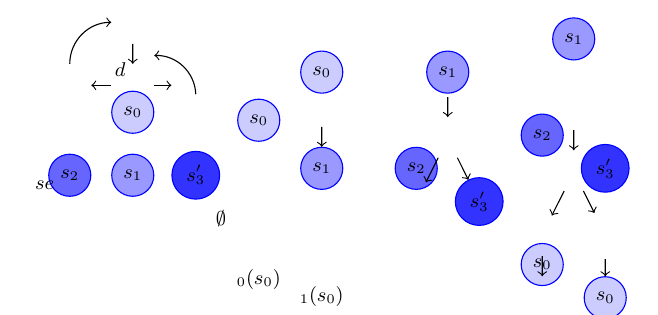
\begin{tikzpicture}[scale=0.8]
				\tikzstyle{every node}=[font=\small,scale=0.8]
				\node[blueCircle] (s0) at(0,1) {$s_0$};
				\node[blueCircle1] (s1) at(0,0) {$s_1$};
				\node[blueCircle2] (s2) at(-1,0) {$s_2$};
				\node[blueCircle3] (s3) at(1,0) {$s_3'$};
				\begin{minipage}{.2\textwidth}
					\draw[->] (s0) -- (s1);
					\draw[->] (s1) -- (s2);
					\draw[->] (s1) -- (s3);
					\path (s2) edge[->,bend right=-45]  (s0);
					\path (s3) edge[->,bend right=45] (s0);
					\node at(-0.2,1.3) {$d$};
					\node at(-1.4,0) {$se$};
					\node at(1.4,0) {$\emptyset$};
					\node at(0,-1.5) {${\cal K}_2$};
					%	\caption{${\cal K}_2$};
				\end{minipage} 
				\begin{minipage} {.2\textwidth}
					\node[blueCircle] (t0) at(2,0.5) {$s_0$};
					\node at(2,-1.5) {$\Tr_0(s_0)$};
				\end{minipage}
				\begin{minipage}{.2\textwidth}
					\node[blueCircle] (t0) at(3,1) {$s_0$};
					\node[blueCircle1] (t1) at(3,0) {$s_1$};
					\draw[->] (t0) -- (t1);
					\node at(3,-1.5) {$\Tr_1(s_0)$};
				\end{minipage}
				\begin{minipage}{.2\textwidth}
					\node[blueCircle] (t0) at(5,2) {$s_0$};
					\node[blueCircle1] (t1) at(5,1) {$s_1$};
					\node[blueCircle2] (t2) at(4.5,0) {$s_2$};
					\node[blueCircle3] (t3) at(5.5,0) {$s_3'$};
					\draw[->] (t0) -- (t1);
					\draw[->] (t1) -- (t2);
					\draw[->] (t1) -- (t3);
					\node at(5,-1.5) {$\Tr_2(s_0)$};
				\end{minipage}
				\begin{minipage}{.2\textwidth}
					\node[blueCircle] (t0) at(7,2) {$s_0$};
					\node[blueCircle1] (t1) at(7,1) {$s_1$};
					\node[blueCircle2] (t2) at(6.5,0) {$s_2$};
					\node[blueCircle3] (t3) at(7.5,0) {$s_3'$};
					\node[blueCircle] (t01) at(6.5,-1) {$s_0$};
					\node[blueCircle] (t02) at(7.5,-1) {$s_0$};
					\draw[->] (t0) -- (t1);
					\draw[->] (t1) -- (t2);
					\draw[->] (t1) -- (t3);
					\draw[->] (t2) -- (t01);
					\draw[->] (t3) -- (t02);
					\node at(7,-1.5) {$\Tr_3(s_0)$};
				\end{minipage}
			\end{tikzpicture}
			\caption{{\footnotesize 初始结构$\mathcal{K}_2$及其计算树示意图}}
		\end{figure}
		%	\begin{figure}
		%		\includegraphics[scale=0.3]{figures/NK2Tree2}
		%		\caption{{\footnotesize 初始结构$\mathcal{K}_2$及其计算树示意图}}\label{fig:K2Tree}
		%	\end{figure}
		%}
		%	\only<2>{  
		%	\begin{block}{计算树互模拟}
		%		给定原子命题集$V\subseteq \Ha$和初始Kripke结构$\Hm_i$($i = 1, 2$)。如果下面条件同时满足:
		%		\begin{itemize}
		%			\item $L_1(s_1)- V=L_2(s_2)- V$, 
		%			\item 对$\Tr_n(s_1)$的任意子树$\Tr_{n-1}(s_1')$,都存在  $\Tr_n(s_2)$的子树$\Tr_{n-1}(s_2')$,使得 
		%			$\Tr_{n-1}(s_1')\lrto_V\Tr_{n-1}(s_2')$,且
		%			\item 对任意$\Tr_n(s_2)$的子树$\Tr_{n-1}(s_2')$,都存在$\Tr_n(s_1)$的子树$\Tr_{n-1}(s_1')$,使得
		%			$\Tr_{n-1}(s_1')\lrto_V\Tr_{n-1}(s_2')$;
		%		\end{itemize}
		%		则称$\Hm_1$的计算树$\Tr_n(s_1)$和$\Hm_2$的计算树$\Tr_n(s_2)$是$V$-互模拟的(记为$({\cal M}_1,\Tr_n(s_1))\lrto_V({\cal M}_2,\Tr_n(s_2))$,简写为$\Tr_n(s_1)\lrto_V\Tr_n(s_2)$)。
		%	\end{block}
		%\begin{proposition}\label{pro:k}
		%	给定原子命题集$V\subseteq \Ha$、初始Kripke结构$\Hm$和两个状态$s,s'\in S$。
		%	若$s\not\lrto_V s'$,则存在一个最小整数$k$,使得$\Tr_k(s)$和$\Tr_k(s')$不是$V$-互模拟的。
		%\end{proposition}
		%}
		%\only<2>{\begin{proposition}\label{pro:k}
		%	给定原子命题集$V\subseteq \Ha$、初始Kripke结构$\Hm$和两个状态$s,s'\in S$。
		%	若$s\not\lrto_V s'$,则存在一个最小整数$k$,使得$\Tr_k(s)$和$\Tr_k(s')$不是$V$-互模拟的。
		%\end{proposition}
		%	}
		%\only<3>{
		%%	\begin{proposition}\label{B_to_T}
		%%		给定原子命题集$V\subseteq\cal A$和结构$({\cal M}_i,s_i)$($i=1,2$)。
		%%		那么:
		%%		\[(s_1,s_2)\in{\cal B}_n\mbox{当且仅当对任意$0\le j\le n$,有}
		%%		\Tr_j(s_1)\lrto_V\Tr_j(s_2)\mbox{。}\]
		%%	\end{proposition}
		%\begin{proposition}\label{pro:k}
		%	给定原子命题集$V\subseteq \Ha$、初始Kripke结构$\Hm$和两个状态$s,s'\in S$。
		%	若$s\not\lrto_V s'$,则存在一个最小整数$k$,使得$\Tr_k(s)$和$\Tr_k(s')$不是$V$-互模拟的。
		%\end{proposition}
		%}
	}
\end{frame}

\begin{frame}
	\frametitle{基于模型的有界CTL遗忘计算——{\footnotesize 描述初始结构: 计算树的特征公式}}
	{\footnotesize 
		%	\only<1>{	
		\begin{definition}\label{def:V:char:formula}
			给定原子命题集$V\subseteq \Ha$、初始Kripke结构$\Hm =(S,R,L,s_0)$和状态$s\in S$。
			定义在$V$上的计算树$\Tr_n(s)$的特征公式(记为${\cal F}_V(\Tr_n(s))$,$n\geq 0$)递归定义如下:
			\begin{align*}
				{\cal F}_V(\Tr_0(s)) &=  \bigwedge_{\textcolor{blue!80}{p \in V\cap L(s)}}p
				\wedge \bigwedge_{\textcolor{blue!80}{q\in V-L(s)}} \neg q,\\
				{\cal F}_V(\Tr_{k+1}(s))& = \bigwedge_{(s,s')\in R}
				\textcolor{blue!80}{\EXIST \NEXT} {\cal F}_V(\Tr_k(s')) 
				\wedge 
				\textcolor{blue!80}{\ALL \NEXT} \bigg( \bigvee_{(s,s')\in R} {\cal F}_V(\Tr_k(s')) \bigg) \wedge {\cal F}_V(\Tr_0(s)) \hbox{ ($k\ge 0$)。}
			\end{align*}
		\end{definition}
		\begin{block}{含义}
			由定义\ref{def:V:char:formula}可知,计算树的特征公式从三个方面展示了计算树的信息:
			\begin{itemize}
				\item[(1)] 只考虑$V$中的原子命题;
				\item[(2)] 突出了树节点的内容,即:对于任意原子命题$p\in V$,若$p$在节点的标签中,则其正出现在特征公式中,否则负出现在特征公式中;
				\item[(3)] 公式中的时序算子表示了状态之间的转换关系。
			\end{itemize}
		\end{block}
		% }
		%	\only<2>{
		%		\begin{lemma}\label{lem:Vb:TrFormula:Equ}
		%			给定原子命题集$V\subseteq \Ha$、初始Kripke结构$\Hm=(S,R,L,s_0)$和$\Hm'=(S',R',L',s_0')$、$s\in S$、$s'\in S'$且 $n\ge 0$。若$\Tr_n(s) \lrto_{\overline V} \Tr_n(s')$,则${\cal F}_V(\Tr_n(s)) \equiv {\cal F}_V(\Tr_n(s'))$。
		%		\end{lemma}
		%	\begin{lemma}\label{Bn:to:Tn}
		%		令$V\subseteq \Ha$、$\Hm=(S, R, L,s_0)$、$\Hm'=(S', R', L',s_0')$、$s\in S$、$s'\in S'$且$n\ge 0$,则:
		%		\begin{itemize}
		%			\item[(i)] $({\cal M},s)\models{\cal F}_V(\Tr_n(s))$;
		%			\item[(ii)] 若$({\cal M},s)\models{\cal F}_V(\Tr_n(s'))$,则
		%			$\Tr_n(s) \lrto_{\overline V} \Tr_n(s')$。
		%		\end{itemize}
		%	\end{lemma}
		%	}
	}
\end{frame}

\begin{frame}
	\frametitle{基于模型的有界CTL遗忘计算——{\footnotesize 描述初始结构:特征公式}}
	{\footnotesize 
		\only<1>{  
			\begin{block}{计算树互模拟}
				给定原子命题集$V\subseteq \Ha$和初始Kripke结构$\Hm_i$($i = 1, 2$)。如果下面条件同时满足:
				\begin{itemize}
					\item $L_1(s_1)- V=L_2(s_2)- V$, 
					\item 对$\Tr_n(s_1)$的任意子树$\Tr_{n-1}(s_1')$,都存在  $\Tr_n(s_2)$的子树$\Tr_{n-1}(s_2')$,使得 
					$\Tr_{n-1}(s_1')\lrto_V\Tr_{n-1}(s_2')$,且
					\item 对任意$\Tr_n(s_2)$的子树$\Tr_{n-1}(s_2')$,都存在$\Tr_n(s_1)$的子树$\Tr_{n-1}(s_1')$,使得
					$\Tr_{n-1}(s_1')\lrto_V\Tr_{n-1}(s_2')$;
				\end{itemize}
				则称$\Hm_1$的计算树$\Tr_n(s_1)$和$\Hm_2$的计算树$\Tr_n(s_2)$是$V$-互模拟的(记为$({\cal M}_1,\Tr_n(s_1))\lrto_V({\cal M}_2,\Tr_n(s_2))$,简写为$\Tr_n(s_1)\lrto_V\Tr_n(s_2)$)。
			\end{block}
			\begin{proposition}\label{pro:k}
				给定原子命题集$V\subseteq \Ha$、初始Kripke结构$\Hm$和两个状态$s,s'\in S$。
				若$s\not\lrto_V s'$,则\textcolor{blue!80}{存在一个最小整数$k$},使得$\Tr_k(s)$和$\Tr_k(s')$不是$V$-互模拟的。
			\end{proposition}
		}
		\only<2>{\begin{block}{$V$-可区分}
				若初始Kripke结构$\Hm$的两个状态$s$和$s'$不是$\overline{V}$-互模拟的(即:$s\not\lrto_{\overline{V}} s'$),则称$s$和$s'$是\emph{$V$-可区分的}。
				用$\dis_V({\cal M},s,s',k)$表示状态$s$和$s'$在命题\ref{pro:k}中所说的最小数$k$下是$V$-可区分的。
			\end{block}
			\begin{block}{特征数}
				$\Hm$关于原子命题集$V$的\emph{特征数},记为$ch({\cal M},V)$定义如下:
				\[ch({\cal M},V)=
				\left\{
				\begin{array}{ll}
					\max\{k\mid s,s'\in S \text{ 且 }\dis_V({\cal M},s,s',k)\}, \qquad \hbox{${\cal M}$是 $V$-可区分的;} \\
					\min\{k\mid {\cal B}_{k}={\cal B}_{k+1}, k\ge 0\}, \ \ \ \quad  \qquad \qquad \qquad \hbox{否则。}
				\end{array}
				\right.
				\]
			\end{block}
		}
		\only<3>{
			%		\begin{lemma}\label{div_s}
			%			令$V\subseteq \Ha$、$\Hm=(S,R,L,s_0)$、$k={ch({\cal M},V)}$且$s\in S$,则
			%			%There is a formula $\phi$ such that
			%			\begin{itemize}
			%				\item[(i)] $(\Hm, s)\models {\cal F}_V(\Tr_k(s))$;
			%				\item[(ii)] 对任意$s'\in S$,$({\cal M},s) \lrto_{\overline V} ({\cal M},s')$当且仅当$({\cal M},s')\models{\cal F}_V(\Tr_k(s))$。
			%			\end{itemize}
			%		\end{lemma}
			\begin{definition}[特征公式]
				给定原子命题集$V\subseteq\cal A$和初始结构${\cal K}=({\cal M},s_0)$,其中$c=ch({\cal M},$ $V)$。对任意$\Hm$上的状态$s' \in S$,记$T(s') = {\cal F}_V(\Tr_c(s'))$。
				$\cal K$关于$V$的{\em 特征公式} ${\cal F}_V({\cal K})$定义为:
				\[T(s_0) \text{ } \wedge \bigwedge_{s\in S}\textcolor{blue!80}{\ALL \GLOBAL}\left(
				T(s) \rto
				\bigwedge_{(s,s')\in R}
				\textcolor{orange!80}{\EXIST \NEXT} T(s')
				\wedge
				\textcolor{orange!80}{\ALL \NEXT} \bigg(\bigvee_{(s,s')\in R}T(s')\bigg)
				\right).
				\]
				
			\end{definition}
			\begin{theorem}\label{CF}
				令$V\subseteq \Ha$、$\Hm=(S,R,L,s_0)$且$\Hm'=(S',R', L',s_0')$,则:
				\begin{itemize}
					\item[(i)] $(\Hm',s_0') \models {\cal F}_V({\cal M},s_0)
					\text{ 当且仅当 }
					({\cal M},s_0) \lrto_{\overline V} ({\cal M}',s_0')$;
					
					\item[(ii)] 若$s_0 \lrto_{\overline V} s_0'$则${\cal F}_V(\Hm, s_0) \equiv {\cal F}_V(\Hm', s_0')$。
				\end{itemize}
				\begin{figure}
					\begin{tikzpicture}
						%	\draw (0,0) rectangle (2,2);
						\node[rectangle, rounded corners =5pt,
						minimum width =50pt ,
						minimum height =30pt ,draw=red, fill=red!20] {相互互模拟的结构的特征公式等价。};
					\end{tikzpicture}
				\end{figure}
			\end{theorem}
		}
		\only<4>{
			{\tiny
				\begin{example}\label{ex:4}
					考虑右下图中左边的初始结构${\cal K}_2= (\Hm, s_0)$。左边的为$\Hm$上的四棵计算树:从左到右表示以$s_0$为根、深度分别为0、1、2和3的计算树(为简化图,计算树的标签没有给出,但是每个树节点的标签可从${\cal K}_2$找到)。令$V=\{d\}$,则 $\overline{V}=\{s, se\}$。
					
					因为$L(s_1) - \overline{V} = L(s_2) - \overline{V}$,所以有$\Tr_0(s_1) \lrto_{\overline{V}} \Tr_0(s_2)$。由于存在$(s_1, s_2)\in R$,使得对任意$(s_2, s') \in R$,都有$L(s_2)- \overline V \neq L(s') - \overline V$,所以,$\Tr_1(s_1) \not \lrto_{\overline{V}} \Tr_1(s_2)$。
					由此可知,$s_1$和$s_2$是$V$-可区分的,且$\dis_{V}(\Hm, s_1, s_2, 1)$。
					
					同理可得:$\dis_{ V}(\Hm, s_0, s_1, 0)$、$\dis_{V}(\Hm, s_1, s_3', 1)$、$\dis_{V}(\Hm, s_0, s_2, 0)$和$\dis_{ V}(\Hm,$ $s_0, s_3', 0)$。此外,$s_2 \lrto_{\overline V} s_3'$。因此,可以计算$\Hm$关于$V$的特征数为:
					$$ch(\Hm, V)=\max\{k\mid s,s'\in S \text{ 且 } \dis_{V}({\cal M},s,s',k)\} = 1.$$ 
					
					所以,可以由以下步骤计算${\cal K}_2$关于$V$的特征公式:
					\begin{columns}
						\column{0.5\textwidth}
						\begin{align*}
							{\cal F}_V(\Tr_0(s_0)) &= d, \qquad \quad {\cal F}_V(\Tr_0(s_1)) = \neg d, \\
							{\cal F}_V(\Tr_0(s_2)) &= \neg d,  \qquad  {\cal F}_V(\Tr_0(s_3')) = \neg d,\\
							{\cal F}_V(\Tr_1(s_0)) &= \EXIST\NEXT \neg d \wedge \ALL\NEXT \neg d \wedge d \equiv \ALL\NEXT \neg d \wedge d, \\
							{\cal F}_V(\Tr_1(s_1)) &= \EXIST\NEXT \neg d \wedge \EXIST\NEXT \neg d  \wedge \ALL\NEXT (\neg d \vee \neg d) \wedge \neg d 
							\equiv \ALL\NEXT \neg d \wedge \neg d, \\
							{\cal F}_V(\Tr_1(s_2)) &= \EXIST\NEXT d  \wedge \ALL\NEXT d \wedge \neg d \equiv \ALL\NEXT d \wedge \neg d,\\
							{\cal F}_V(\Tr_1(s_3')) &\equiv {\cal F}_V(\Tr_1(s_2)),\\
							{\cal F}_V(\Hm, s_0)&\equiv \ALL\NEXT \neg d \wedge d \wedge \\
							& \ALL \GLOBAL(\ALL\NEXT \neg d \wedge d \rto \ALL\NEXT(\ALL\NEXT \neg d \wedge \neg d))\wedge \\
							& \ALL \GLOBAL(\ALL\NEXT \neg d \wedge \neg d \rto \ALL\NEXT(\ALL\NEXT d \wedge \neg d)) \wedge\\
							& \ALL \GLOBAL(\ALL\NEXT d \wedge \neg d \rto \ALL\NEXT(\ALL\NEXT \neg d \wedge d)).
						\end{align*}
						\column{0.5\textwidth} 
						\begin{figure}
							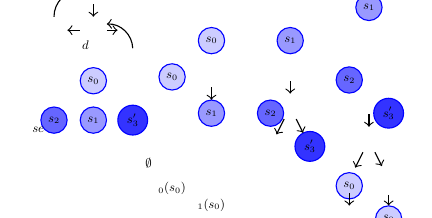
\begin{tikzpicture}[scale=0.5]
								\tikzstyle{every node}=[font=\small,scale=0.5]
								\node[blueCircle] (s0) at(0,1) {$s_0$};
								\node[blueCircle1] (s1) at(0,0) {$s_1$};
								\node[blueCircle2] (s2) at(-1,0) {$s_2$};
								\node[blueCircle3] (s3) at(1,0) {$s_3'$};
								\begin{minipage}{.2\textwidth}
									\draw[->] (s0) -- (s1);
									\draw[->] (s1) -- (s2);
									\draw[->] (s1) -- (s3);
									\path (s2) edge[->,bend right=-45]  (s0);
									\path (s3) edge[->,bend right=45] (s0);
									\node at(-0.2,1.3) {$d$};
									\node at(-1.4,0) {$se$};
									\node at(1.4,0) {$\emptyset$};
									\node at(0,-1.5) {${\cal K}_2$};
									%	\caption{${\cal K}_2$};
								\end{minipage} 
								\begin{minipage} {.2\textwidth}
									\node[blueCircle] (t0) at(2,0.5) {$s_0$};
									\node at(2,-1.5) {$\Tr_0(s_0)$};
								\end{minipage}
								\begin{minipage}{.2\textwidth}
									\node[blueCircle] (t0) at(3,1) {$s_0$};
									\node[blueCircle1] (t1) at(3,0) {$s_1$};
									\draw[->] (t0) -- (t1);
									\node at(3,-1.5) {$\Tr_1(s_0)$};
								\end{minipage}
								\begin{minipage}{.2\textwidth}
									\node[blueCircle] (t0) at(5,2) {$s_0$};
									\node[blueCircle1] (t1) at(5,1) {$s_1$};
									\node[blueCircle2] (t2) at(4.5,0) {$s_2$};
									\node[blueCircle3] (t3) at(5.5,0) {$s_3'$};
									\draw[->] (t0) -- (t1);
									\draw[->] (t1) -- (t2);
									\draw[->] (t1) -- (t3);
									\node at(5,-1.5) {$\Tr_2(s_0)$};
								\end{minipage}
								\begin{minipage}{.2\textwidth}
									\node[blueCircle] (t0) at(7,2) {$s_0$};
									\node[blueCircle1] (t1) at(7,1) {$s_1$};
									\node[blueCircle2] (t2) at(6.5,0) {$s_2$};
									\node[blueCircle3] (t3) at(7.5,0) {$s_3'$};
									\node[blueCircle] (t01) at(6.5,-1) {$s_0$};
									\node[blueCircle] (t02) at(7.5,-1) {$s_0$};
									\draw[->] (t0) -- (t1);
									\draw[->] (t1) -- (t2);
									\draw[->] (t1) -- (t3);
									\draw[->] (t2) -- (t01);
									\draw[->] (t3) -- (t02);
									\node at(7,-1.5) {$\Tr_3(s_0)$};
								\end{minipage}
							\end{tikzpicture}
							\caption{{\tiny 初始结构$\mathcal{K}_2$及其计算树示意图}}\label{fig:K2Tree}
						\end{figure}
						%				\begin{figure}
						%					\includegraphics[scale=0.25]{figures/NK2Tree2}
						%					\caption{{\tiny 初始结构$\mathcal{K}_2$及其计算树示意图}}\label{fig:K2Tree}
						%				\end{figure}
					\end{columns} 
				\end{example}
			}
		} 
	}
\end{frame}

\begin{frame}
	\frametitle{基于模型的有界CTL遗忘计算——{\footnotesize 计算WSC}}
	{\footnotesize 
		\begin{example}[例~\ref{exam:SNCandWSC}的延续]
			%\label{exam:SNCandWSC}
			令$\Ha=\{d,se,sp,s\}$和$V=\{d,se\}$,求$s$在$V$和初始结构${\cal K} = (\Hm,s_0)$ 上的WSC,其中$\Hm$为例~\ref{car_manufacturing}中初始状态为$s_0$的汽车制造企业模型结构。
			
			$s$在$V$和初始结构${\cal K} = (\Hm,s_0)$上的WSC为$\neg \CTLforget({\cal F}_{\Ha}({\cal K}) \wedge \neg s, \{s\}$ $\cup \{sp\})$。
			{\tiny 
				\begin{columns}
					\column{0.5\textwidth}
					\begin{align*}
						&	\CTLforget({\cal F}_{\Ha}({\cal K}) \wedge \neg s, \{s\} \cup \{sp\})\\
						&	\equiv \CTLforget(\CTLforget({\cal F}_{\Ha}({\cal K}) \wedge \neg s, \{sp\}), \{s\})\\
						&	\equiv \CTLforget(\CTLforget({\cal F}_{\Ha}({\cal K}), \{sp\})\wedge \neg s, \{s\}).
					\end{align*}
					
					\qquad  $\CTLforget({\cal F}_{\Ha}({\cal K}), \{sp\}) \equiv {\cal F}_{V\cup \{s\}}({\cal K})$\\
					\qquad  所以要计算$\neg \CTLforget({\cal F}_{\Ha}({\cal K}) \wedge \neg s,$ $\{s\}\cup \{sp\})$,\\
					\qquad  只需计算$\neg \CTLforget({\cal F}_{V\cup \{s\}}({\cal K})\wedge \neg s, \{s\})$。\\
					\qquad 令$V' = V \cup \{s\} = \{d,se,s\}$,\\
					\qquad  则$\overline{V'} = \{sp\}$。
					\column{0.5\textwidth}
					\begin{align*}
						&\neg \CTLforget({\cal F}_{V\cup \{s\}}({\cal K})\wedge \neg s, \{s\}) \\
						& \equiv \neg \CTLforget({\cal F}_{V\cup \{s\}}({\cal K}), \{s\})\\
						& \equiv \neg \CTLforget(\psi \wedge \ALL \GLOBAL(\varphi_1 \wedge \varphi_2 \wedge \varphi_3\wedge \varphi_4),\{s\})\\	
						& \equiv \neg(\CTLforget(\psi \wedge \varphi_1 \wedge \varphi_2 \wedge \varphi_3\wedge \varphi_4, \{s\}) \wedge \ALL \GLOBAL \CTLforget(\varphi_1 \wedge \varphi_2 \wedge \varphi_3\wedge \varphi_4, \{s\}))\\
						& \equiv  \neg \bigg(\Big(d \vee \big((d\vee se) \wedge \ALL\NEXT(d \wedge \neg se)\big) \vee \big((d \vee se \vee \ALL\NEXT \neg d) \wedge\\
						& \EXIST\NEXT(\neg d \wedge se) \wedge \EXIST\NEXT(\neg d \wedge \neg se)\big) \\
						& \vee (d \wedge \ALL\NEXT(\neg d \wedge \neg se)) \vee \big((d\vee \neg se) \wedge \EXIST\NEXT\neg d\big) \Big) \wedge\\
						& \ALL \GLOBAL\Big(\big((d \vee se) \wedge \ALL\NEXT(d \wedge \neg se)\big) \vee \big(\ALL\NEXT \neg d \wedge \EXIST\NEXT(\neg d \wedge se) \wedge\\
						& \EXIST\NEXT(\neg d \wedge \neg se)\big) \vee \big((d\vee se) \wedge \ALL\NEXT(\neg d \wedge \neg se)\big) \vee \EXIST\NEXT \neg d\Big)
						\bigg).
					\end{align*}
				\end{columns} 
			}
		\end{example}
	}
\end{frame}


\begin{frame}
	\frametitle{遗忘封闭性}
	{\footnotesize 
		\begin{lemma}\label{lem:models:formula}
			给定$\CTL$公式$\varphi$,下面等式成立:
			\begin{equation*}
				\varphi\equiv \bigvee_{(\Hm, s_0)\in\Mod(\varphi)}{\cal F}_{\cal A}(\Hm, s_0).
			\end{equation*}
		\end{lemma}
		\begin{block}{遗忘封闭性}
			从$\varphi$中遗忘$V$中的元素得到的结果为:
			\begin{equation*}
				\bigvee_{{\cal K}\in  \{{\cal K}'\mid \exists {\cal K}''\in\Mod(\phi),\ {\cal K}''\lrto_V{\cal K}'\}} {\cal F}_{\overline V}({\cal K}).
			\end{equation*}
		\end{block}
	}
\end{frame}

\begin{frame}
	\frametitle{基于模型的遗忘算法}
	{\footnotesize 
		\begin{figure}
			\includegraphics[scale=0.45]{figures/model-basedAlg}
		\end{figure}
		
		\begin{proposition}\label{pro:time:alg1}
			令 $\varphi$为$\CTL$公式,$V\subseteq \Ha$为原子命题集,状态空间大小为 $|{\cal S}|=m$, $|\Ha|=n$,$|V|=x$。使用算法5.1计算从$\varphi$中遗忘$V$中原子的空间复杂度为 $O((n-x)m^{2(m+2)}2^{nm}  \log m)$,且时间复杂性至少与空间复杂性相同。
		\end{proposition}
	}
\end{frame}

\begin{frame}
	\frametitle{遗忘复杂性}
	{\footnotesize 
		%	\only<1>{	\begin{lemma}\label{lem:models:formula}
		%			给定$\CTL$公式$\varphi$,下面等式成立:
		%			\begin{equation*}
		%				\varphi\equiv \bigvee_{(\Hm, s_0)\in\Mod(\varphi)}{\cal F}_{\cal A}(\Hm, s_0).
		%			\end{equation*}
		%		\end{lemma}
		%	\begin{block}{遗忘封闭性}
		%		从$\varphi$中遗忘$V$中的元素得到的结果为:
		%		\begin{equation*}
		%			\bigvee_{{\cal K}\in  \{{\cal K}'\mid \exists {\cal K}''\in\Mod(\phi),\ {\cal K}''\lrto_V{\cal K}'\}} {\cal F}_{\overline V}({\cal K}).
		%		\end{equation*}
		%	\end{block}}
		%	\only<2>{
		$\CTL_{\ALL\FUTURE}$:表示$\CTL$公式只包含时序算子$\ALL \FUTURE$的子类。
		\begin{proposition}[模型检测]
			\label{modelChecking}
			给定一个结构 $(\Hm,s_0)$、原子命题集$V\subseteq{\cal A}$和公式 $\varphi \in \CTL_{\ALL\FUTURE}$,判定 $(\Hm,s_0)$ 是否为$\CTLforget(\varphi, V)$的模型是 \textsc{NP}-完全的。
		\end{proposition}
		\begin{theorem}[Entailment]
			\label{thm:comF}
			令 $\varphi$和 $\psi$为$\CTL_{\ALL \FUTURE}$中的两个公式, $V$为原子命题集。则:
			\begin{itemize}
				\item[(i)] 判定  $\CTLforget(\varphi, V ) \models^? \psi$是 co-$\textsc{NP}$-完全的,
				\item[(ii)] 判定  $\psi \models^? \CTLforget(\varphi, V)$是 $\Pi_2^{\textsc{P}}$-完全的,
				\item[(iii)] 判定 $\CTLforget(\varphi, V) \models^? \CTLforget(\psi, V)$是 $\Pi_2^{\textsc{P}}$-完全的。
			\end{itemize}
		\end{theorem}
		\begin{corollary}
			令 $\varphi$和 $\psi$为 $\CTL_{\ALL \FUTURE}$中的两个公式,$V$原子公式集。则
			\begin{itemize}
				\item[(i)] 判定 $\psi \equiv^?\CTLforget(\varphi, V)$是 $\Pi_2^{\textsc{P}}$-完全的,
				\item[(ii)] 判定 $\CTLforget(\varphi, V) \equiv^? \varphi$是 co-$\textsc{NP}$-完全的,
				\item[(iii)] 判定 $\CTLforget(\varphi, V) \equiv^? \CTLforget(\psi, V)$是$\Pi_2^{\textsc{P}}$-完全的。
			\end{itemize}
		\end{corollary}
		%	}
	}
\end{frame}

%\begin{frame}
%	\frametitle{基于模型的遗忘算法}
%	{\footnotesize 
%		\begin{figure}
%			\includegraphics[scale=0.45]{figures/model-basedAlg}
%		\end{figure}
%	
%	\begin{proposition}\label{pro:time:alg1}
%		令 $\varphi$为$\CTL$公式,$V\subseteq \Ha$为原子命题集,状态空间大小为 $|{\cal S}|=m$, $|\Ha|=n$,$|V|=x$。使用算法5.1计算从$\varphi$中遗忘$V$中原子的空间复杂度为 $O((n-x)m^{2(m+2)}2^{nm}  \log m)$,且时间复杂性至少与空间复杂性相同。
%	\end{proposition}
%	}
%\end{frame}

\subsection{基于归结的遗忘计算方法}
\begin{frame}
	\frametitle{基于归结的算法CTL-forget——{\footnotesize 总体框架}}
	{\footnotesize
		\begin{figure}
			\centering
			% Requires \usepackage{graphicx}
			\includegraphics[scale=0.5]{figures/frame2}\\
			\caption{基于归结的遗忘的主要流程图}
			\label{Fig:chapter05:v1uv2}
		\end{figure}
		\pause
		\begin{itemize}
			\item 如何表示$\CTL$公式和带索引的$\CTL$公式之间的关系?
			\item 如何“移除”无关的原子命题(包括需要遗忘的原子命题和转换过程中引入的新的原子命题),以及如何“消除”索引?
		\end{itemize}
	}
\end{frame}

\begin{frame}
	\frametitle{基于归结的算法CTL-forget——{\footnotesize CTL归结UF}}
	{\footnotesize
		\only<1>{
			\begin{table}[tb]%[width=.9\linewidth,cols=4,pos=h]
				\scriptsize
				%	\small
				\centering
				\caption{$R_{\CTL}^{\succ,S}$归结系统}\label{tab:res}
				\begin{tabular}{l}
					\toprule
					$
					\begin{aligned}
						& \textbf{(SRES1)}\frac{P\rto \ALL\NEXT(C\vee l), Q\rto \ALL\NEXT(D\vee \neg l)}{P\wedge Q \rto \ALL\NEXT(C\vee D)};
						&& \textbf{(SRES2)} \frac{P\rto \EXIST_{\tuple{ind}} \NEXT(C\vee l), Q\rto \ALL\NEXT(D\vee \neg l)}{P\wedge Q \rto \EXIST_{\tuple{ind}}\NEXT(C\vee D)};\\
						& \textbf{(SRES3)} \frac{P\rto \EXIST_{\tuple{ind}}\NEXT(C\vee l), Q \rto \EXIST_{\tuple{ind}}\NEXT(D\vee \neg l)}{P\wedge Q\rto\EXIST_{\tuple{ind}}\NEXT(C\vee D)};  
						&&   \textbf{(SRES4)} \frac{\start \rto C\vee l, \start \rto D \vee \neg l}{\start \rto C\vee D}; \\
						& \textbf{(SRES5)} \frac{\top \rto C\vee l, \start \rto D \vee \neg l}{\start \rto C \vee D};
						&&  \textcolor{blue!80}{\textbf{(SRES6)} \frac{\top \rto C \vee l, Q \rto \ALL\NEXT(D \vee \neg l)}{Q\rto \ALL \NEXT(C\vee D)}}; \\
						& \textbf{(SRES7)} \frac{\top \rto C \vee l, Q \rto \EXIST_{\tuple{ind}} \NEXT(D \vee \neg l)}{Q\rto \EXIST_{\tuple{ind}}\NEXT(C\vee D)}; 
						&&  \textbf{(SRES8)} \frac{\top \rto C\vee l, \top \rto D \vee \neg l}{\top \rto C \vee D};\\
						& \textbf{(RW1)} \frac{\bigwedge_{i=1}^n m_i \rto \ALL\NEXT \perp}{\top \rto \bigvee_{i=1}^n \neg m}; 
						&& \textbf{(RW2)} \frac{\bigwedge_{i=1}^n m_i \rto \EXIST_{\tuple{ind}}\NEXT \perp}{\top \rto \bigvee_{i=1}^n \neg m}; \\
						& \textbf{(ERES1)} \frac{\Lambda \rto \EXIST \NEXT \EXIST\GLOBAL l, Q \rto \ALL \FUTURE \neg l}{Q \rto \ALL(\neg \Lambda \UNLESS \neg l)};
						&& \textbf{(ERES2)} \frac{\Lambda \rto \EXIST_{\tuple{ind}} \NEXT \EXIST_{\tuple{ind}}\GLOBAL l, Q \rto \EXIST_{\tuple{ind}} \FUTURE \neg l}{Q \rto \EXIST_{\tuple{ind}}(\neg \Lambda \UNLESS \neg l)}.
					\end{aligned}
					$\\
					\bottomrule
				\end{tabular}
			\end{table}
			其中$P$和$Q$是文字的合取,$C$和$D$是文字的析取,$l$是一个文字,称每条规则横线下面的公式为横线上面的公式关于文字$l$的归结结果。此外,$\Lambda=\bigvee_{i=1}^n \bigwedge_{i=1}^{m_i}P_j^i$、$P_j^i$是文字的析取,其中$1\leq i\leq n$和$1\leq j\leq m$。
		}
		\only<2>{	\begin{block}{记号}
				\begin{itemize}
					\item 令$T$为$\CTLsnf$子句集,$p$为原子命题。$T$在$p$上的\emph{展开}(记为$\Unfolding(T,p)$)是集合$T$和如下集合的并集:
					\[\{\alpha\mid \mbox{$\alpha$ 是 $T$ 中的公式关于文字 $l\in\{p,\neg p\}$ 的归结结果}\}.  \]
					\item $\Unfolding(T,\emptyset)=T$且$\Unfolding(T,\{p\}\cup V)=\Unfolding(\Unfolding(T,p), V)$;
					\item $\emph{ERes}(\varphi,V) = \{\alpha\in \Unfolding(T_\varphi,V)\mid \Var(\alpha)\cap V=\emptyset\}$。
				\end{itemize}
			\end{block}
			\begin{proposition}\label{pro:resEQ}
				令 $\varphi$ 为一个 $\CTL$公式,$V\subseteq\cal A$为原子命题集。则
				$T_\varphi \equiv_U\emph{ERes}(\varphi,V)$,其中  $U=\Var(\Unfolding(T_\varphi,V))-(\Var(\varphi)-  V)$。
		\end{proposition}}
		\only<3>{\tiny
			\begin{example}\label{examp:Res} 
				令 $\varphi=\ALL((p\wedge q) \UNTILL (f\vee m)) \wedge r$,\textcolor{orange!80}{$V=\{p,r\}$},则  $\Unfolding(T_\varphi, V\cup \{x,y,z\})$ 除了$T_{\varphi}$中的子句,
				\begin{align*}
					&  1: \start\rto z, &&  2: \textcolor{orange!80}{\top \rto \neg z \vee r}, &&  3:\top \rto \neg x\vee f \vee m, &&
					4: \top \rto y \vee x \vee \neg z, \\
					&  5: \textcolor{orange!80}{\top \rto p \vee \neg y}, &&  6: \top \rto \neg y \vee q, &&  7:  z \rto \ALL \FUTURE x, &&  8: y \rto \ALL \NEXT(y \vee x).
				\end{align*}
				还包含如下子句: 
				\begin{align*}
					&(1)\ \textcolor{orange!80}{\start \rto r} && (1,2,\textbf{SRES5})
					&&(2)\ \start \rto x \vee y && (1,4,\textbf{SRES5})\\
					% \end{align*}
					% \begin{align*}
					&(3)\ \top \rto \neg z \vee y \vee f \vee m && (3, 4, \textbf{SRES8})
					&&(4)\ y \rto \ALL\NEXT(f\vee m\vee y) && (3,8, \textbf{SRES6})\\
					&(5)\ \textcolor{orange!80}{\top \rto \neg z \vee x \vee p} && (4,5, \textbf{SRES8})
					&&(6)\ \top \rto \neg z \vee x \vee q && (4,6, \textbf{SRES8})\\
					&(7)\ \textcolor{orange!80}{y \rto \ALL\NEXT(x\vee p)} && (5, 8, \textbf{SRES6})
					&&(8)\ y \rto \ALL\NEXT(x\vee q) && (6, 8, \textbf{SRES6})\\
					&(9)\ \start \rto f\vee m \vee y && (3,(2), \textbf{SRES5})
					% \end{align*}
					% \begin{align*}
					&&(10)\ \textcolor{orange!80}{\start \rto x \vee p} && (5,(2),\textbf{SRES5}) \\
					&(11)\ \start \rto x \vee q && (6,(2), \textbf{SRES5})
					&& (12)\ \textcolor{orange!80}{\top \rto p \vee \neg z \vee f \vee m} && (5,(3), \textbf{SRES8})\\
					& (13)\ \top \rto q \vee \neg z \vee f \vee m && (6,(3), \textbf{SRES8})
					&&(14)\ \textcolor{orange!80}{y \rto \ALL\NEXT(p \vee f\vee m)} && (5, (4), \textbf{SRES6})\\
					& (15)\ \textcolor{blue!80}{y \rto \ALL\NEXT(q \vee f\vee m)} && (6, (4), \textbf{SRES6})
					%\end{align*}
					%\begin{align*}
					&&(16)\ \textcolor{orange!80}{\start \rto f\vee m \vee p} && (5, (9), \textbf{SRES5}) \\
					&(17)\ \start \rto f\vee m \vee q && (6, (9), \textbf{SRES5})
				\end{align*}
				
				在从 $\Unfolding(T_\varphi, V\cup \{x,y,z\})$中移除包含 $V$中元素的子句后,得到 $\emph{ERes}(\varphi,V)$,其包含如下子句:
				\begin{align*}%{llll}
					&\start\rto z, \quad \start \rto f\vee m \vee q, \quad  \start \rto x \vee y, \quad \start \rto q \vee x, \quad	\start \rto f\vee m \vee y, \\
					& \top \rto f \vee m \vee \neg x, \quad		\top \rto q \vee f \vee m\vee \neg z,
					\quad  	\top \rto f \vee m \vee \neg z \vee y,\\
					& \top \rto q \vee x\vee \neg z, \quad 	\top \rto x \vee y \vee \neg z, \quad 	\top \rto q\vee\neg y , \quad z \rto \ALL \FUTURE x, \\
					& y \rto \ALL\NEXT(q \vee f\vee m), \quad  y \rto \ALL\NEXT(x\vee q), \quad y \rto \ALL \NEXT(x\vee y),\quad 	y \rto \ALL\NEXT(f\vee m\vee y).
				\end{align*}
				
				可以看出,尽管 $\emph{ERes}(\varphi,V)$中不包含具有索引的公式,但有的子句包含出现在 $T_\varphi$中的新原子命题。
			\end{example}
		}
	}
\end{frame}

\begin{frame}
	\frametitle{基于归结的算法CTL-forget——{\footnotesize 转子句为CTL公式}}
	{\footnotesize
		\only<1>{	
			\begin{block}{两个主要过程}
				\begin{itemize}
					\item 消除索引;
					\item 移除新引入的原子命题。
				\end{itemize} 
			\end{block} 
			\begin{lemma} 
				如果$j\in {\cal I}$,$\psi_i,\varphi_i~(1\le i\le n)$为 $\CTL$公式,那么:
				\begin{itemize}
					\item[(i)] $\{\psi_i\rto \EXIST_{\tuple{j}} \NEXT \varphi_i \mid 1\le i\le n\}\equiv 
					\{\left(\bigwedge_{i\in S}\psi_i\right)\rto \EXIST_{\tuple{j}} \NEXT \left(\bigwedge_{i\in S}\varphi_i\right)\mid S\subseteq\{1,\dots, n\}\}$,
					
					\item[(ii)] $\{\psi_i\rto \EXIST_{\tuple{j}} \NEXT \varphi_i \mid 1\le i\le n\}\equiv_\emptyset
					\{\left(\bigwedge_{i\in S}\psi_i\right)\rto \EXIST \NEXT \left(\bigwedge_{i\in S}\varphi_i\right)\mid S\subseteq\{1,\dots, n\}\}$,
					
					\item[(iii)] $\{(\psi_1 \rto \EXIST_{\tuple{j}}\FUTURE \varphi_1), (\psi_2 \rto \EXIST_{\tuple{j}}\NEXT \varphi_2)\}$ 
					$\equiv_\emptyset$ 
					\begin{equation*}
						(\psi_1 \rto \varphi_1 \vee \EXIST \NEXT \EXIST \FUTURE \varphi_1)
						\wedge (\psi_2 \rto \EXIST \NEXT \varphi_2)
						\wedge (\psi_1 \wedge \psi_2 \rto ((\varphi_1 \wedge \EXIST \NEXT \varphi_2) \vee \EXIST \NEXT (\varphi_2 \wedge \EXIST \FUTURE \varphi_1))).
					\end{equation*}
				\end{itemize}
			\end{lemma} 
		}
		\only<2>{
			\begin{columns}
				\column{0.7\textwidth}
				\begin{figure}
					\includegraphics[scale=0.4]{figures/removeInd1}
				\end{figure}
				
				\column{0.3\textwidth}
				{\tiny \textcolor{blue!80}{$rei(\{\alpha_i\mid 1\le i\le n\})$、
						$rxi(\{\alpha_i\mid 1\le i\le n\})$、$rfi(\{\beta_1,\alpha_2\})$分别表示引理30中(i)、(ii)、(iii)等号 $\equiv_*$($* \in \{$空字符串,$\emptyset\}$)的右边,$\alpha_i=\psi_i\rto \EXIST_{\tuple{j}} \NEXT \varphi_i$ $(1\le i\le n)$且$\beta_1=\psi_1 \rto \EXIST_{\tuple{j}}\FUTURE \varphi_1$。}
				}
			\end{columns}
			%		\begin{figure}
			%			\includegraphics[scale=0.45]{figures/removeInd}
			%		\end{figure}
			%	{\tiny 其中,$rei(\{\alpha_i\mid 1\le i\le n\})$、
			%	$rxi(\{\alpha_i\mid 1\le i\le n\})$、$rfi(\{\beta_1,\alpha_2\})$分别表示引理33中(i)、(ii)、(iii)等号 $\equiv_*$($* \in \{$空字符串,$\emptyset\}$)的右边,$\alpha_i=\psi_i\rto \EXIST_{\tuple{j}} \NEXT \varphi_i$ $(1\le i\le n)$且$\beta_1=\psi_1 \rto \EXIST_{\tuple{j}}\FUTURE \varphi_1$。}
			\begin{corollary}
				如果$\varphi$为一个$\CTL$公式、$U=\Var(T_\varphi)-\Var(\varphi)$,$V\subseteq\cal A$为原子命题集、
				$\Sigma=\emph{ERes}(\Unfolding(\varphi,V\cup U),V)$,那么
				RM-index$(\Sigma)\equiv_\emptyset \Sigma$。
			\end{corollary}
			\begin{lemma}[一般化的Ackermann引理] \label{thm:Aclm}
				令 $x$为一个原子命题、 
				% 	$\Delta = \{\top \rto \neg x \vee C_1$, \dots, $\top \rto \neg x \vee C_n, x \rto B_1, \dots, x \rto B_m\}$
				% 	be a set of $\CTLsnf$ clauses
				$\Delta = \{\ALL\GLOBAL(\top \rto \neg x \vee C_1)$, $\dots$, $\ALL\GLOBAL(\top \rto \neg x \vee C_n), \ALL\GLOBAL(x \rto B_1), \dots, \ALL\GLOBAL(x \rto B_m)\}$为只包含一个$x$的$\CTL$公式集($n, m \geq 1$)、
				$\Gamma$为 $x$正出现在其中的有限个$\CTL$公式集。下面式子成立:
				\begin{equation}\label{eq:Ackermann:lemma}
					\Gamma\cup \Delta \equiv_{\{x\}}  
					\Gamma\left[x/\bigwedge\left(\{C_i\mid 1\le i\le n\}\cup\{B_i\mid 1\le i\le m\}\right)\right].
				\end{equation}
			\end{lemma}
		}
		%\only<3>{
		%	\begin{lemma}[一般化的Ackermann引理,Generalised Ackermann's Lemma] \label{thm:Aclm}
		%		令 $x$为一个原子命题、 
		%		% 	$\Delta = \{\top \rto \neg x \vee C_1$, \dots, $\top \rto \neg x \vee C_n, x \rto B_1, \dots, x \rto B_m\}$
		%		% 	be a set of $\CTLsnf$ clauses
		%		$\Delta = \{\ALL\GLOBAL(\top \rto \neg x \vee C_1)$, $\dots$, $\ALL\GLOBAL(\top \rto \neg x \vee C_n), \ALL\GLOBAL(x \rto B_1), \dots, \ALL\GLOBAL(x \rto B_m)\}$为只包含一个$x$的$\CTL$公式集($n, m \geq 1$)、
		%		$\Gamma$为 $x$正出现在其中的有限个$\CTL$公式集。下面式子成立:
		%		\begin{equation}\label{eq:Ackermann:lemma}
		%			\Gamma\cup \Delta \equiv_{\{x\}}  
		%			\Gamma\left[x/\bigwedge\left(\{C_i\mid 1\le i\le n\}\cup\{B_i\mid 1\le i\le m\}\right)\right].
		%		\end{equation}
		%	\end{lemma}
		%	}
		
		\only<3>{
			\begin{example}[例30的延续]
				\label{examp:Aclm}
				首先考虑原子命题 \textcolor{blue!80}{$x$、 $\Delta=\{\top \rto f \vee m \vee \neg x\}$和 $\Gamma=\emph{ERes}(\varphi,V)-\Delta$}。
				$\Gamma$中包含$x$的公式关于$x$都为正的,因此 $\Gamma[x/(f \vee m)]$包含如下公式:
				\begin{align*}%{llll}
					& \start\rto z, \quad \start \rto f\vee m \vee q, \quad  \start \rto f \vee m \vee y, \\
					% \quad \start \rto q \vee f \vee m, \quad	\start \rto f\vee m \vee y, \\
					%& \top \rto q \vee f \vee m\vee \neg z,   \quad  	\top \rto f \vee m \vee \neg z \vee y,\\
					& \top \rto q \vee f \vee m \vee \neg z, \quad 	\top \rto f \vee m \vee y \vee \neg z,
					\quad \top \rto q\vee\neg y , \quad z \rto \ALL \FUTURE (f \vee m), \\
					& y \rto \ALL\NEXT(q \vee f\vee m), %\quad  y \rto \ALL\NEXT(f \vee m\vee q), %\quad y \rto \ALL \NEXT(f \vee m\vee y),
					\quad 	y \rto \ALL\NEXT(f\vee m\vee y).
				\end{align*}
				
				第二步考虑原子命题\textcolor{blue!80}{ $z$、
					$\Delta'=\{ \top \rto q \vee f \vee m \vee \neg z, \top \rto f \vee m \vee y \vee \neg z ,z \rto \ALL \FUTURE (f \vee m)\}$
					和 $\Gamma'=\Gamma[x/(f \vee m)] -\Delta'$,其中$z$正出现在$\Gamma'$中}。因此,
				$\Gamma''=\Gamma'[z/ (q \vee f \vee m)\land (f \vee m \vee y)\land\ALL \FUTURE (f \vee m)]$包含如下公式:
				\begin{align*}%{llll}
					& \start\rto  (q \vee f \vee m)\land (f \vee m \vee y)\land\ALL \FUTURE (f \vee m),
					\quad \start \rto f\vee m \vee q, \quad  \start \rto f \vee m \vee y,  \\
					&  \top \rto q\vee\neg y,  \quad y \rto \ALL\NEXT(q \vee f\vee m), \quad y \rto \ALL\NEXT(f\vee m\vee y).
				\end{align*}
				
				不难证明$\emph{ERes}(\varphi,V)\equiv_{\{x,z\}} \Gamma''$。
				因为$\Gamma''$包含一个公式,\textcolor{orange!80}{其关于$y$既不是正的也不是负的。因此,这里不能对$\Gamma''$和 $y$使用上述过程。} 
			\end{example}
		}
	}
\end{frame}

\begin{frame}
	\frametitle{基于归结的算法CTL-forget及其复杂性}
	{\footnotesize
		
		\only<1>{
			
			\begin{figure}
				\includegraphics[scale=0.42]{figures/CTL-forget1}
			\end{figure}
			%		}
			%		\only<2>{	
			\begin{theorem}[可靠性]\label{thm:soundness:forget:algorithm}
				若$\varphi$为一个$\CTL$公式、 $V\subseteq\cal A$、 $\Sigma=$\CTL-forget$(\varphi,V)$且$U=\Var(\Sigma)-\Var(\varphi)$,则:
				\begin{itemize}
					\item[(i)] $\Sigma\equiv_{V\cup U}\varphi$,
					\item[(ii)] 若$U=\emptyset$,则 $\Sigma\equiv\CTLforget(\varphi,V)$。
				\end{itemize}
			\end{theorem}
			
			\begin{proposition}\label{pro:complexity}
				给定$\CTL$公式$\varphi$和原子命题集$V \subseteq \Ha$。
				算法5.3的时间和空间复杂性为{\em $O((m+1)2^{4(n+n')})$},其中$n=|\Var(\varphi)|$、$n'=|V'|$为新引入的原子命题的个数、$m$为引入的索引个数。
			\end{proposition}
		}
		\only<2>{
			\begin{example}[例31的延续]\label{examp:forget:algorithm}
				容易看出 \CTL-forget$(\varphi,\{p,r\})$包含下面的公式
				\begin{align*}%{llll}
					&  (q \vee f \vee m)\land (f \vee m \vee y)\land\ALL \FUTURE (f \vee m), \quad \ALL\GLOBAL ( \top \rto q\vee\neg y),  \\
					&  \ALL\GLOBAL(y \rto \ALL\NEXT(q \vee f\vee m)), \quad \ALL\GLOBAL( y \rto \ALL\NEXT(f\vee m\vee y)).
				\end{align*}
			\end{example}
			\begin{proposition}[遗忘存在的子类]\label{pro:fogCTL}
				给定$\CTL$公式$\varphi$,若$\varphi$满足下面约束:
				(1)$\varphi$中不包括操作符$Pt {\cal T}$(其中$Pt \in \{\ALL, \EXIST\}$且${\cal T} \in \{\UNTILL, \GLOBAL\}$);(2)对于任意原子命题$p\in V$, 若$p$和$\neg p$出现在同一时序算子的范围内。
				那么,$\emph{CTL-forget}(\varphi,V) \equiv \CTLforget(\varphi, V)$。
			\end{proposition}
		} 
	}
\end{frame}

\end{document}